% ------------------------------------------------------------------------
% ------------------------------------------------------------------------
% ICMC: Modelo de Trabalho Acadêmico (tese de doutorado, dissertação de
% mestrado e trabalhos monográficos em geral) em conformidade com 
% ABNT NBR 14724:2011: Informação e documentação - Trabalhos acadêmicos -
% Apresentação
% ------------------------------------------------------------------------
% ------------------------------------------------------------------------
% Opções:
%   Qualificação          = qualificacao 
%   Curso                 = doutorado/mestrado
%   Situação do trabalho  = pre-defesa/pos-defesa (exceto para qualificação)
%   Versão para impressão = impressao
\documentclass[doutorado, pos-defesa]{packages/icmc}
% ---------------------------------------------------------------------------
% Pacotes Opcionais
% ---------------------------------------------------------------------------
\usepackage{rotating}           % Usado para rotacionar o texto
\usepackage[all,knot,arc,import,poly]{xy}   % Pacote para desenhos gráficos
% Este pacote pode conflitar com outros pacotes gráficos como o ``pictex''
% Então é necessário usar apenas um dos pacotes conflitantes
\newcommand{\VerbL}{0.52\textwidth}
\newcommand{\LatL}{0.42\textwidth}
% ---------------------------------------------------------------------------
%%%%%%%% Novos pacotes adicionados
\usepackage{tikz}
\usepackage{multicol}
\usepackage{multirow}
\usepackage{longtable}
\usepackage{threeparttablex}
\usepackage{array}
\usepackage{subcaption}
\usepackage{comment}
% ---------------------------------------------------------------------------
% Informações de dados para CAPA e FOLHA DE ROSTO
% ---------------------------------------------------------------------------
% Tanto na capa quanto nas folhas de rosto apenas a primeira letra da primeira palavra (ou nomes próprios) devem estar em letra maiúscula, todas as demais devem ser em letra minúscula.
\tituloPT{Verificação de Código de Simulação Numérica de Escoamentos de Fluidos Viscoelásticos Através do Método de Soluções Manufaturadas}

\tituloEN{Verification of Numerical Simulation Code for Viscoelastic Fluid Flows Using the Manufactured Solution Method}

\autor[Organista, J.]{Juniormar Organista}
\genero{M} % Gênero do autor (M = Masculino / F = Feminino)
\orientador[Orientador]{Prof. Dr.}{Leandro Franco de Souza}
%\coorientador{Prof. Dr.}{Fulano de Tal}
\curso{CCMC}
\data{27}{03}{2025} % Data do depósito
\idioma{PT} % Idioma principal do documento (PT = português / EN = inglês)
% ---------------------------------------------------------------------------
% ---------------------------------------------------------------------------
% Verificação de Código de Simulação Numérica de Escoamentos de Fluidos Viscoelásticos Através do Método de Soluções Manufaturadas
% Aplicação do Método das Soluções Manufaturadas para Escoamento Viscoelástico Incompressível
% RESUMOS
% ---------------------------------------------------------------------------
% Resumo em PORTUGUÊS
% conter no máximo 500 palavras
% conter no mínimo 1 e no máximo 5 palavras-chave
\textoresumo[brazil]{
    Este trabalho apresenta uma abordagem utilizando um método de discretização de alta ordem, baseado em esquemas compactos de diferenças finitas, para a solução das equações bidimensionais de escoamento viscoelástico incompressível na formulação vorticidade-função de corrente. A verificação da precisão e robustez dos esquemas numéricos foi realizada por meio do Método das Soluções Manufaturadas (MMS), utilizando como caso de referência o escoamento em cavidade com tampa móvel. O MMS, amplamente utilizado para validação de códigos numéricos, permite a criação de soluções analíticas artificiais que compartilham as mesmas equações e condições de contorno do problema simulado, sendo uma ferramenta eficaz para avaliar a precisão, convergência e estabilidade de códigos numéricos. Este método foi aplicado a quatro modelos constitutivos amplamente usados na modelagem de fluidos viscoelásticos: UCM (Upper Convected Maxwell), LPTT (Linear Phan-Thien-Tanner), Oldroyd-B e Giesekus. Para os modelos Oldroyd-B e Giesekus, as simulações consideraram números de Reynolds ($Re$) variando de 1 a 1000, diferentes razões de viscosidade do solvente ($\beta_{nn} = 0.1,\ 0.5,\ 0.9$ e $1.0$), com o número de Weissenberg variando entre $1$, $5$ e $10$. No caso do modelo Giesekus, o parâmetro de anisotropia do tensor de tensões, $\alpha_G$, foi variado entre 0.1 e 0.5, enquanto no modelo LPTT o parâmetro $\epsilon$ foi analisado para diferentes cenários de elasticidade. As simulações realizadas com o modelo UCM, que se caracteriza pela simplicidade de seu tratamento da elasticidade, também foram avaliadas quanto à sua capacidade de capturar fenômenos viscoelásticos em escoamentos complexos. Os resultados indicam que o código numérico desenvolvido apresenta uma ordem de convergência próxima de 4.5, em linha com as previsões teóricas para métodos de alta ordem. A precisão e robustez dos métodos foram validadas pela consistente redução dos erros à medida que a malha foi refinada, independente do modelo constitutivo, número de Reynolds, ou razão de viscosidade do solvente. Para fluidos newtonianos ($\beta_{nn} = 1$), os erros se aproximaram dos níveis de precisão de máquina, confirmando que os esquemas numéricos lidam corretamente com simplificações do modelo. Além disso, o modelo Giesekus demonstrou ser estável e preciso para toda a faixa de valores de $\alpha_G$, e o modelo LPTT, com diferentes valores de $\epsilon$, também mostrou boa adaptação a regimes variados de elasticidade. O modelo UCM, mesmo sendo mais simples, foi capaz de lidar com os desafios numéricos dos escoamentos viscoelásticos simulados. Em conclusão, o uso do MMS comprovou ser uma ferramenta poderosa na verificação e validação de códigos numéricos aplicados à simulação de escoamentos viscoelásticos. O desempenho consistente dos esquemas numéricos implementados, aliado à validação por meio de soluções manufaturadas, assegura a confiabilidade dos resultados obtidos, tornando esses métodos adequados para a modelagem de fluidos não newtonianos em cenários complexos. Além disso, os dados e as tabelas de erros apresentados garantem a reprodutibilidade dos experimentos e a aplicabilidade dos métodos desenvolvidos em futuras pesquisas acadêmicas.
    }{Fluidos Viscoelásticos, Método das Soluções Manufaturadas, Discretização de Alta Ordem, Simulação Numérica, Modelos Constitutivos Viscoelásticos}
% ---------------------------------------------------------------------------
% resumo em INGLÊS
% conter no máximo 500 palavras
% conter no mínimo 1 e no máximo 5 palavras-chave
\textoresumo[english]{
    This work presents an approach utilizing a high-order discretization method based on compact finite difference schemes for solving the two-dimensional incompressible viscoelastic flow equations in the vorticity-stream function formulation. The accuracy and robustness of the numerical schemes were verified using the Method of Manufactured Solutions (MMS), with the lid-driven cavity flow as the reference case. MMS, widely used for validating numerical codes, allows for the creation of artificial analytical solutions that share the same governing equations and boundary conditions as the simulated problem, making it an effective tool for evaluating the accuracy, convergence, and stability of numerical codes. This method was applied to four constitutive models commonly used in viscoelastic fluid modeling: UCM (Upper Convected Maxwell), LPTT (Linear Phan-Thien-Tanner), Oldroyd-B, and Giesekus. For the Oldroyd-B and Giesekus models, simulations considered Reynolds numbers ($Re$) ranging from 1 to 1000 and different solvent viscosity ratios ($\beta_{nn} = 0.0,\ 0.1,\ 0.5,\ 0.9$, and $1.0$), with the Weissenberg ranging from 1, 5 and 10. In the Giesekus model, the anisotropy parameter of the stress tensor, $\alpha_G$, was varied between 0.1 and 0.5, while in the LPTT model, the parameter $\epsilon$ was analyzed across different elasticity scenarios. Simulations performed with the UCM model, known for its simplicity in handling elasticity, were also evaluated for their ability to capture viscoelastic phenomena in complex flows. The results indicate that the developed numerical code exhibits a convergence order close to 4.5, consistent with theoretical predictions for high-order methods. The accuracy and robustness of the methods were validated by the consistent reduction of errors as the mesh was refined, regardless of the constitutive model, Reynolds number, or solvent viscosity ratio. For Newtonian fluids ($\beta_{nn} = 1$), the errors approached machine precision levels, confirming that the numerical schemes correctly handle model simplifications. Additionally, the Giesekus model proved to be stable and accurate across the entire range of $\alpha_G$ values, and the LPTT model, with different values of $\epsilon$, also showed good adaptability to various elasticity regimes. The UCM model, despite being simpler, effectively managed the numerical challenges posed by the simulated viscoelastic flows. In conclusion, the use of MMS proved to be a powerful tool for verifying and validating numerical codes applied to viscoelastic flow simulations. The consistent performance of the implemented numerical schemes, coupled with validation through manufactured solutions, ensures the reliability of the results obtained, making these methods suitable for modeling non-Newtonian fluids in complex flow scenarios. Furthermore, the provided data and error tables ensure the reproducibility of the experiments and the applicability of the developed methods in future academic research.
    }{Viscoelastic Fluids, Method of Manufactured Solutions, High-Order Discretization, Numerical Simulation, Viscoelastic Constitutive Models}
% ---------------------------------------------------------------------------
% ELEMENTOS PRÉ-TEXTUAIS
% ---------------------------------------------------------------------------
% Inserir a ficha catalográfica
\incluifichacatalografica{tex/pre-textual/ficha-catalografica.pdf}
% DEDICATÓRIA / AGRADECIMENTO / EPÍGRAFE
\textodedicatoria*{tex/pre-textual/dedicatoria}
\textoagradecimentos*{tex/pre-textual/agradecimentos}
\textoepigrafe*{tex/pre-textual/epigrafe}
% ---------------------------------------------------------------------------
% Inclui a lista de figuras
\incluilistadefiguras
% ---------------------------------------------------------------------------
% Inclui a lista de tabelas
\incluilistadetabelas
% ---------------------------------------------------------------------------
% Inclui a lista de quadros
% \incluilistadequadros
% ---------------------------------------------------------------------------
% Inclui a lista de algoritmos
\incluilistadealgoritmos
% ---------------------------------------------------------------------------
% Inclui a lista de códigos
\incluilistadecodigos
% ---------------------------------------------------------------------------
% Inclui a lista de siglas e abreviaturas
\incluilistadesiglas
% ---------------------------------------------------------------------------
% Inclui a lista de símbolos
\incluilistadesimbolos
% ---------------------------------------------------------------------------
% Início do documento
% ---------------------------------------------------------------------------
\begin{document}
% ---------------------------------------------------------------------------
% ELEMENTOS TEXTUAIS
% ---------------------------------------------------------------------------
\textual
% ---------------------------------------------------------------------------
% Capítulo 1 - Introdução
% ---------------------------------------------------------------------------
% ----------------------------------------------------------
%% Capitulo1-Introducao.tex
% ----------------------------------------------------------
% Introducao 
% ----------------------------------------------------------
\chapter[Introdução]{Introdução}
\label{Cap_Introducao}

Em diversas aplicações industriais, a dinâmica dos fluidos desempenha um papel central na eficiência e qualidade dos processos. Produtos industriais que envolvem o escoamento de fluidos, como o processamento de polímeros, a injeção de plásticos e a extração de petróleo, frequentemente dependem de fluidos com propriedades complexas, como os fluidos viscoelásticos. Esses fluidos, que combinam características de fluidos viscosos e sólidos elásticos, representam um desafio na modelagem e simulação devido à sua resposta não linear ao estresse e à deformação. Essa complexidade torna essencial o uso de métodos numéricos avançados e de alta precisão para prever o comportamento desses fluidos em diferentes condições. A substituição de materiais poliméricos por alternativas mais eficientes é uma prática comum em setores industriais, como a indústria automotiva, que busca otimizar processos e reduzir custos. Um estudo de caso relevante na indústria automobilística demonstrou a importância de selecionar adequadamente materiais poliméricos com propriedades específicas para aplicações exigentes, como a resistência ao impacto em baixas temperaturas e a compatibilidade com os processos de fabricação existentes \cite{bissoto2006substituiccao}. Esse cenário destaca a crescente necessidade de compreender o comportamento de escoamentos viscoelásticos em condições variadas, garantindo que o desempenho mecânico dos polímeros seja mantido ao longo da vida útil dos produtos. Assim, a compreensão e o controle dos escoamentos viscoelásticos tornam-se cruciais para assegurar a qualidade e a durabilidade dos produtos derivados de polímeros em diversas indústrias.

Na literatura, encontram-se diversos estudos que abordam modelos constitutivos para fluidos viscoelásticos, como as equações diferenciais de Maxwell \cite{beris1987spectral,mompean97}, Oldroyd-B \cite{brasseur1998time,mompean97,phillips2002,pinho2003}, White-Metzner \cite{White63}, Giesekus \cite{giesekus1962, giesekus1982, giesekus1985}, Leonov \cite{Leonov76}, modelos FENE\sigla*{FENE}{\textit{Finite Extensible Nonlinear Elastic}} \cite{Bird80,Bird83,christiansen77,Stevenson71,Warner72}, PTT \cite{phan-thien77,pinho2003}\sigla*{PTT}{Phan-Thien-Tanner} e derivados, Pom-Pom \cite{Larson88} e os modelos integrais: Maxwell \cite{Kaye62} e K-BKZ\sigla*{K-BKZ}{Kaye-Bernstein-Kearsley-Zapas} \cite{luo88}. 

O modelo de Maxwell foi uma das primeiras abordagens para descrever a viscoelasticidade em fluidos, combinando as propriedades de um sólido elástico de Hooke com as de um fluido viscoso newtoniano. Já o modelo Oldroyd-B, derivado da teoria cinética para soluções poliméricas concentradas e fundidas \cite{bird_v1_1987}, representa a cadeia polimérica como duas esferas conectadas por uma mola, onde as esferas correspondem ao centro de massa do sistema e as molas simulam a elasticidade das macromoléculas. Esse modelo é particularmente eficaz para representar fluidos com elasticidade ideal, como os fluidos Boger.

O modelo reológico proposto por \citeonline{giesekus1982} também se fundamenta em abordagens moleculares, utilizando sistemas compostos por esferas e molas, em que a mola segue a lei de Hooke. Diferentemente do modelo Oldroyd-B, o modelo Giesekus incorpora um efeito de anisotropia na formulação da força de arrasto que atua sobre as esferas. Isso resulta em uma equação similar aos modelos UCM\sigla{UCM}{\textit{Upper Convected Maxwell}} e Oldroyd-B, mas com a inclusão de termos não lineares, decorrentes dos produtos envolvendo o tensor de tensões. Outro modelo amplamente aplicado em simulações numéricas de fluidos viscoelásticos é o proposto por \citeonline{phan-thien77}, conhecido como PTT, que tem suas bases na teoria de redes de soluções concentradas e polímeros fundidos, levando em conta a energia elástica dessas redes.

Essas simulações ainda tem a vantagem de poder fornecer resultados precisos que representam com fidelidade o comportamento desses fluidos em diferentes cenários de escoamento. Contudo, a complexidade desse problema reside nas equações constitutivas que governam os fluidos viscoelásticos, tornando seu tratamento computacional desafiador. Com o desenvolvimento da tecnologia computacional, o interesse por simulações numéricas dessas aplicações industriais cresceu, uma vez que métodos numéricos permitem a modelagem de escoamentos de fluidos viscoelásticos com um custo significativamente menor do que em relação aos experimentos laboratoriais, proporcionando resultados precisos e que capturam o comportamento dos fluidos viscoelásticos sob diferentes condições. No entanto, essas simulações enfrentam desafios consideráveis, pois as equações constitutivas que descrevem esses fluidos são complexas e difíceis de tratar computacionalmente. Nesse contexto, a Dinâmica dos Fluidos Computacional (CFD, do inglês: \textit{Computational Fluid Dynamics})\sigla*{CFD}{\textit{Computational Fluid Dynamics}} se destaca como uma ferramenta indispensável para garantir a confiabilidade dos resultados gerados pelos métodos numéricos, e assim é fundamental realizar processos de Verificação e Validação. Esses procedimentos asseguram a precisão e a credibilidade das soluções encontradas. Conforme indicado pelo o Comitê Americano de Aeronáutica e Astronáutica (AIAA, do inglês:\textit{American Institute of Aeronautics and Astronautics})\sigla*{AIAA}{\textit{American Institute of Aeronautics and Astronautics}}\cite{AIAA2002} em seu guia, elaborado em 1998, para realização da Verificação e da Validação de códigos e resultados obtidos. Segundo \citeonline{oberkampftech}, esses processos envolvem a aplicação de conceitos e práticas rigorosas que garantem a correta implementação e confiabilidade dos códigos computacionais utilizados.

Os conceitos de Verificação e Validação, embora distintos, são complementares e sinérgicos, como apontado por \citeonline{oberkampftech}. A execução de um não elimina a necessidade do outro. De acordo com \citeonline{roacheartigo}, a Validação busca avaliar a precisão de uma simulação ao compará-la com dados experimentais disponíveis na literatura para o caso estudado. Já a Verificação, conforme também destacado por \citeonline{roacheartigo}, concentra-se em verificar se o código numérico executa corretamente os modelos implementados, avaliando a ordem de precisão e os erros numéricos com base em comparações com soluções conhecidas. Diferente da Validação, a Verificação não se preocupa com a correspondência entre o modelo e o mundo real, mas sim com a exatidão do processo de cálculo. Embora este trabalho reconheça a importância da Validação, será focado exclusivamente em testes de Verificação. Para mais detalhes sobre o processo de Validação, o leitor pode consultar as obras de \cite{roacheartigo} e \cite{oberkampftech}.

A verificação de código é fundamental na modelagem computacional, pois permite avaliar a precisão e a confiabilidade dos códigos numéricos aplicados na simulação de fenômenos físicos complexos \cite{Khoshghalb2019, Tranquilli2022}. Esse processo consiste em comparar os resultados obtidos pelo código com soluções analíticas conhecidas ou casos de referência que já possuem soluções estabelecidas \cite{Fernandes2018, Pedro2020}. Ao realizar a verificação, os pesquisadores garantem que os códigos estão corretamente implementados e são capazes de gerar resultados precisos. Esse processo é crucial para assegurar que o código capture de forma adequada a física do problema em análise. Além disso, a verificação permite identificar e corrigir possíveis erros ou inconsistências na implementação, garantindo que as simulações numéricas resultem em dados confiáveis e coerentes. Também auxilia na detecção das limitações dos métodos numéricos empregados, orientando o desenvolvimento de algoritmos mais robustos e precisos.

O Método das Soluções Manufaturadas (MMS, do inglês: \textit{Method of Manufactured Solution})\sigla*{MMS}{\textit{Method of Manufactured Solution}} tem um papel fundamental na verificação e validação de códigos computacionais voltados para a simulação de escoamentos de fluidos viscoelásticos \cite{Garcia2022}. Devido ao comportamento reológico complexo desses fluidos, a simulação numérica precisa apresenta desafios significativos \cite{Fernandes2017}. Em seu estudo, \citeonline{Tseng2021} investigaram o transiente de sobretensão em derretimentos poliméricos sob escoamento de cisalhamento inicial, analisando a eficiência da equação constitutiva de White-Metzner para captar variações expressivas na sobretensão em números elevados de Weissenberg. Os resultados numéricos para o coeficiente de crescimento da tensão de cisalhamento, em diversas taxas de cisalhamento, mostraram uma boa concordância com dados experimentais, corroborando a precisão do modelo. Por sua vez, \citeonline{Pimenta2019} implementaram solucionadores acoplados para simulações de escoamentos viscoelásticos transientes e em regime permanente, com acionamento elétrico, dentro da abordagem de volumes finitos, concluindo que solucionadores acoplados proporcionam maior precisão em simulações transientes e permitem o uso de passos de tempo maiores sem divergência numérica.

Já \citeonline{Fernandes2022} desenvolveram um método acoplado totalmente implícito para a resolução de escoamentos laminares, incompressíveis, não isotérmicos e viscoelásticos, utilizando a estrutura do tensor de conformação-log para números elevados de Weissenberg. O algoritmo foi validado ao ser aplicado em escoamentos de fluidos viscoelásticos Oldroyd-B não isotérmicos em problemas de referência envolvendo uma geometria de contração abrupta planar 4:1, tanto bidimensional quanto axissimétrica. Um dos problemas de referência frequentemente utilizado para validar novos métodos numéricos é o escoamento em cavidade com tampa móvel, que consiste no movimento da parede superior de um canal quadrangular, gerando um escoamento 2D \cite{Shankar2000}. Utilizando essa configuração, \citeonline{Abuga2020} apresentaram tanto resultados de validação quanto novos dados de referência para escoamentos viscoelásticos governados pelo modelo constitutivo Rolie-Poly, utilizando um solucionador baseado em volumes finitos de segunda ordem no OpenFOAM. Além disso, \citeonline{Fernandes2019} aplicaram o escoamento em cavidade com tampa móvel para avaliar o desempenho de seu algoritmo totalmente acoplado de segunda ordem em escoamentos laminares e incompressíveis com malhas colocalizadas. Similarmente, \citeonline{Tomio2020} validaram seu esquema numérico recém-desenvolvido, que emprega uma abordagem de diferenças finitas totalmente implícita de segunda ordem para discretizar os termos de convecção e difusão das equações governantes, utilizando a configuração de escoamento em cavidade com tampa móvel.

Esquemas de discretização de alta ordem são fundamentais na modelagem computacional, oferecendo diversas vantagens em relação aos métodos tradicionais de primeira e segunda ordens. Tais esquemas proporcionam maior precisão, permitindo a obtenção de soluções mais confiáveis e exatas para problemas complexos. Eles são capazes de capturar com eficiência características de pequenas escalas e gradientes acentuados, além de reduzir erros numéricos relacionados à dissipação e dispersão \cite{Souza2005}. Por exemplo, \citeonline{Souza2005} avaliaram o desempenho de diferentes esquemas de diferenças finitas na simulação de ondas de instabilidade em um escoamento bidimensional incompressível, utilizando uma formulação baseada na função corrente-vorticidade. Quatro esquemas de discretização espacial foram comparados, incluindo métodos de segunda a sexta ordem, sendo a integração no tempo realizada por um esquema de Runge-Kutta de quarta ordem. A análise demonstrou a superioridade dos esquemas de alta ordem na captura de fenômenos de instabilidade no escoamento.

De forma semelhante, \citeonline{Cueto2006} propuseram uma abordagem inovadora utilizando aproximações de quadrados mínimos móveis (MLS, do inglês: \textit{Moving Least Squares})\sigla*{MLS}{\textit{Moving Least Squares}} para desenvolver discretizações de volumes finitos de alta ordem em malhas não estruturadas. Essa técnica foi aplicada às equações de águas rasas, destacando-se pela sua precisão e flexibilidade, especialmente na modelagem de fluxos viscosos. Além disso, \citeonline{Silva2010} conduziram um teste de verificação com um código de Simulação Numérica Direta (DNS, do inglês: \textit{Direct Numerical Simulation})\sigla*{DNS}{Direct Numerical Simulation}, que utilizava esquemas de alta ordem e o Método das Soluções Manufaturadas, focado na evolução de ondas de instabilidade em escoamento de Poiseuille plano. O estudo comparou esquemas compactos e não compactos de alta ordem, bem como métodos espectrais, demonstrando sua eficácia.

Em outro trabalho, \citeonline{Fadel2011} desenvolveram um esquema de alta ordem baseado em diferenças finitas para resolver as equações de Stokes e Navier-Stokes incompressíveis, aplicando estênceis de alta ordem para gradientes de pressão e condições de contorno variadas. O método foi testado em diversos problemas bidimensionais, como escoamentos de Stokes, cavidade com tampa móvel e degrau recuado, destacando-se pela precisão e robustez. Além disso, \citeonline{ZHANG2019634} introduziram um esquema de alta ordem para reinicialização do método de conjunto de nível, comprovando sua eficácia em simulações de dinâmicas de interface, como a ruptura de gotas suspensas.

Por fim, \citeonline{ALMUSHAIRA2021235} apresentaram um método numérico de alta ordem estável e eficiente para resolver equações de reação-difusão fracionárias. Utilizando um esquema compacto de quarta ordem e a técnica de transferência matricial, juntamente com a Transformada Rápida de Fourier (FFT, do inglês: \textit{Fast Fourier Transform})\sigla*{FFT}{\textit{Fast Fourier Transform}}, o estudo demonstrou o desempenho da abordagem em modelos complexos, como Fitzhugh-Nagumo, Allen-Cahn, e Schnakenberg, mostrando precisão e estabilidade para problemas de reação-difusão tridimensionais.

Este trabalho tem como principal objetivo desenvolver uma Solução Manufaturada para a verificação de um código numérico utilizado na simulação de escoamentos de fluidos viscoelásticos, com foco nos modelos constitutivos UCM, Oldroyd-B, Giesekus e LPTT\sigla{LPTT}{\textit{Linear Phan-Thien-Tanner}}. A implementação da MMS permitirá avaliar a precisão e a exatidão do código, assegurando que os termos fontes introduzidos nas equações governantes sejam corretamente incorporados e processados. Com a verificação bem-sucedida, será possível garantir que o código numérico está adequado para resolver com rigor as equações desses modelos viscoelásticos complexos. Uma vez finalizado o processo de verificação, os termos fontes adicionados durante os testes poderão ser removidos, restabelecendo o código à sua forma original, de modo que ele possa ser utilizado em outras simulações e pesquisas realizadas pelo grupo. Assim, o presente trabalho não só reforça a confiabilidade do código em uso, mas também contribui para o avanço nas simulações numéricas de escoamentos de fluidos viscoelásticos, assegurando a robustez necessária para futuros estudos.

\section{Organização do trabalho}
Esta tese está organizada da seguinte forma:

No Capítulo \ref{Cap_FormulacaoMatematica} apresenta-se as equações governantes para os escoamentos incompressíveis de fluidos viscoelásticos, abrangendo os modelos constitutivos UCM, Oldroyd-B, Giesekus e LPTT. Neste capítulo, também são discutidos os processos de adimensionalização dessas equações, destacando os parâmetros adimensionais críticos, como o número de Weissenberg, que influenciam o comportamento dos fluidos viscoelásticos e o número Reynolds. A adimensionalização é essencial para garantir a generalidade dos resultados e facilitar a análise comparativa entre os diferentes modelos.

No Capítulo \autoref{Cap_MetodosNumericos} abordam-se os métodos numéricos utilizados para a solução das equações governantes. São detalhados os esquemas de discretização espacial e temporal, como diferenças finitas e métodos implícitos, além dos algoritmos implementados para resolver os sistemas de equações que descrevem os escoamentos viscoelásticos. A precisão e eficiência dos métodos numéricos são discutidas neste contexto.

O Capítulo \ref{Cap_MetodosSolucoesManufaturadas} é dedicado ao Método das Soluções Manufaturadas utilizado para a verificação do código numérico. Este capítulo descreve em detalhes o procedimento de geração dos termos fontes, necessários para a implementação da MMS e explica como essa técnica é empregada para verificar a ordem de convergência do código em relação aos modelos UCM, Oldroyd-B, Giesekus e LPTT.

No Capítulo \ref{Cap_ResultadosNumericos} apresenta-se os resultados obtidos a partir da verificação do código utilizando a Solução Manufaturada. Os resultados são discutidos em termos de precisão numérica, erros relativos e eficiência do código ao tratar os diferentes modelos constitutivos. Além disso, são avaliadas as implicações dos testes realizados sobre a robustez do código e sua aplicabilidade em simulações futuras.

No Capítulo traz-se as conclusões deste trabalho, enfatizando a importância da verificação numérica para garantir a confiabilidade de simulações de escoamentos de fluidos viscoelásticos. O capítulo também sugere possíveis melhorias no código e direções para trabalhos futuros.

No Apêndice \ref{chapter:mathematica_wolfran}, são apresentados os códigos utilizados para a geração dos termos fontes, que foram empregados na Solução Manufaturada e no Apêndice \ref{chapter:fortran_77} são apresentados os códigos em Fortran 77 que são resultados do caso que utilizamos neste trabalho. Esses códigos servem como referência para futuras implementações e adaptações.
% ---------------------------------------------------------------------------
% ---------------------------------------------------------------------------
% Capítulo 2 - Formulação
% ---------------------------------------------------------------------------
% ----------------------------------------------------------
%% Capitulo2-Formulacao.tex
% ----------------------------------------------------------
% Formulacao Matematica 
% ----------------------------------------------------------
\chapter[Formulação]{Formulação Matemática}
\label{Cap_FormulacaoMatematica}

Neste capítulo, são apresentadas as formulações matemáticas que governam os escoamentos incompressíveis e isotérmicos de fluidos viscoelásticos e dependentes do tempo. Para esse tipo de escoamento, utiliza-se uma combinação das equações de conservação de massa, quantidade de movimento, além de uma equação constitutiva que descreve o comportamento não newtoniano do fluido. Também são apresentadas as adimensionalizações das equações.

\section{Equações Governantes}\label{Sec:EquacoesGovernantes}
Escoamentos incompressíveis e isotérmicos são governados pela equação de continuidade, que assegura a conservação da massa:
\begin{equation}\label{eq_conservacao_massa}
    \nabla\cdot\mathbf{u} = 0,
\end{equation}
e pela equação de quantidade de movimento, que representa a conservação de momentum:
\begin{equation}\label{eq_conservacao_momentum}
    \rho \left( \frac{\partial \mathbf{u}}{\partial t} + \nabla \cdot (\mathbf{u} \mathbf{u}) \right) = \nabla \cdot \sigma,
\end{equation}
onde $\rho$\simbolo{\rho}{densidade} é a massa específica do fluido (densidade), $\mathbf{u}$\simbolo{\mathbf{u}}{vetor de velocidade} é o vetor de velocidade, $t$\simbolo{t}{tempo} é o tempo e o operador $\nabla = \left(\frac{\partial}{\partial x_{1}},\frac{\partial}{\partial x_{2}},\cdots,\frac{\partial}{\partial x_{n}}\right)$. A variável $\sigma$\simbolo{\sigma}{tensor de tensões totais} é o tensor de tensões totais, definido por:
\begin{equation}\label{eq_tensoes_totais}
    \sigma = \tau - p \mathbf{I},
\end{equation}
onde $p$\simbolo{p}{pressão} é a pressão, $\mathbf{I}$\simbolo{\mathbf{I}}{tensor identidade} é o tensor identidade, e $\tau$\simbolo{\tau}{tensor de tensões extra-simétrico} é o tensor de tensões extra-simétrico, definido pela equação constitutiva do fluido considerado. A tensão interna do fluido depende da natureza do fluido e pode ser descrita por diferentes modelos constitutivos, dependendo se o fluido é newtoniano ou não. 

Para fluidos newtonianos, o tensor de tensões $\tau$ é proporcional ao tensor taxa de deformação $\mathbf{D}$\simbolo{\mathbf{D}}{tensor taxa de deformação}, conforme a relação linear:
\begin{equation}\label{eq_tensoes_totais_newtoniano}
    \tau = 2 \mu_s \mathbf{D},
\end{equation}
onde $\mu_s$ é a viscosidade dinâmica do fluido e $\mathbf{D}$ é o tensor taxa de deformação, dado por:
\begin{equation}\label{eq_taxa_deformacao_newtoniano}
    \mathbf{D} = \frac{1}{2}(\nabla \mathbf{u} + \nabla\mathbf{u}^{T} ).
\end{equation}

Em contrapartida, para fluidos não newtonianos, como os fluidos viscoelásticos, a relação entre as tensões e a deformação é mais complexa. O comportamento das tensões em função da deformação pode incluir efeitos elásticos e de afinamento por cisalhamento. Para fluidos não newtonianos, o tensor de tensões $\tau$ não exibe linearidade entre a taxa de deformação e a tensão de cisalhamento. O valor da viscosidade dinâmica não é constante, ou seja, varia com a taxa de deformação aplicada \cite{tanner1988}. Para fluidos não newtonianos, o tensor extra-tensões simétrico é definido como a soma da contribuição newtoniana (viscosa) e da contribuição não newtoniana (elástica) \cite{RAJAGOPALAN1990}, que é dado por:
\begin{equation}\label{eq_tensoes_totais_nao_newtoniano}
    \tau=2 \mu_s D+T,
\end{equation}
onde $\mu_s$ é a viscosidade do solvente newtoniano, $D$ é o tensor taxa de deformação definido pela Equação \eqref{eq_taxa_deformacao_newtoniano} e $T$ é o tensor extra-tensão (simétrico) que representa a contribuição não newtoniana do fluido.

Portanto, ao calcular a divergência do tensor de tensões totais $(\sigma)$ da Equação \eqref{eq_tensoes_totais_nao_newtoniano}, a equação de quantidade de movimento para um fluido viscoelástico obtida é dada por:
\begin{equation}
    \begin{split}
        \rho \left( \frac{\partial \mathbf{u}}{\partial t} + \nabla \cdot (\mathbf{uu}) \right) = -\nabla p + \mu_s \nabla^2 \mathbf{u} + \nabla \cdot \mathbf{T}.
    \end{split}\label{eq_conservacao_momentum_nao_newtoniano}
\end{equation}

Neste trabalho, a equação constitutiva $LPOG$ foi adotada para a modelagem do comportamento de fluidos viscoelásticos. Essa formulação é originalmente apresentada por \citeonline{furlan2022linear}, onde é construída como uma síntese das contribuições de diversos trabalhos relevantes na área, incluindo os estudos de \citeonline{beris1987spectral}, \citeonline{brasseur1998time}, \citeonline{phan-thien77} e \citeonline{giesekus1982}. A equação LPOG se destaca por combinar os efeitos de deformação viscosa e elástica em um único modelo. De forma geral, a equação é expressa como:
\begin{equation}
    \begin{split}
        \left( 1 + \frac{\epsilon \lambda}{\mu_p} \textbf{tr}(\mathbf{T}) \right) \mathbf{T} + \lambda \left(\frac{\partial \mathbf{T}}{\partial t} + \mathbf{u} \cdot \nabla \mathbf{T} - \mathbf{T} \cdot\nabla \mathbf{u} - \nabla \mathbf{u}^T \cdot \mathbf{T} \right) + \frac{\alpha_G \lambda}{\mu_p} (\mathbf{T} \cdot \mathbf{T}) + \\ + \xi\lambda (\mathbf{D} \cdot \mathbf{T} + \mathbf{T} \cdot \mathbf{D}) = 2 \mu_p \mathbf{D},
    \end{split}\label{eq_tensores_lpog}
\end{equation}
onde $\mu_p$\simbolo{\mu_p}{coeficiente de viscosidade polimérica} é o coeficiente de viscosidade polimérica, $\lambda$\simbolo{\lambda}{tempo de relaxação do fluido} representa o tempo de relaxação do fluido, e $\alpha_G$\simbolo{\alpha_G}{parâmetro de mobilidade } é o parâmetro de mobilidade que regula o comportamento de afinamento por cisalhamento do fluido ($0 \leq \alpha_G \leq 0,5$), sendo este um parâmetro característico do modelo de Giesekus. A origem do termo relacionado a $\alpha_G$  pode ser associada ao arrasto hidrodinâmico anisotrópico sobre as moléculas poliméricas constituintes \cite{bird_v1_1987}. O parâmetro $\xi$ é uma constante positiva do modelo PTT e está relacionado às diferenças nas tensões normais. Já o parâmetro $\epsilon$ está vinculado ao comportamento elongacional do fluido, impedindo a ocorrência de uma viscosidade elongacional infinita em um fluxo de estiramento simples, como aconteceria em um modelo de Maxwell (UCM ou Oldroyd-B) quando $\epsilon = 0$ \cite{pinho2000axial}. Esse parâmetro $\epsilon$ descreve as propriedades extensionais do fluido, onde, quanto maior a oposição ao alongamento axial de um filamento fluido, menor será o valor de $\epsilon$. O termo $\textbf{tr}(\mathbf{T})$ representa o traço do tensor $T$, enquanto $T\cdot T$ denota o produto tensorial.

Assim na equação constitutiva denominada LPOG \eqref{eq_tensores_lpog}, é possível derivar quatro modelos viscoelásticos distintos. Para cada modelo, basta realizar as seguintes substituições:
\begin{itemize}
    \item Modelo UCM: $\alpha_G = \xi = \epsilon = 0$ ($\mu_s = 0$); 
    \item Modelo Oldroyd-B: $\alpha_G = \xi = \epsilon = 0$;
    \item Modelo de Giesekus: $\xi = \epsilon = 0$;
    \item Modelo LPTT: $\alpha_G = 0$.
\end{itemize}

\section{Equações Adimensionais}\label{Sec:Adimensionalizacao}
As equações \eqref{eq_conservacao_massa} - \eqref{eq_conservacao_momentum_nao_newtoniano} descrevem o comportamento de escoamentos viscoelásticos incompressíveis e isotérmicos, tendo sido inicialmente apresentadas em sua forma dimensional. Entretanto, é mais vantajoso resolvê-las na forma adimensional, pois isso facilita a compreensão dos efeitos físicos envolvidos, além de permitir que o modelo seja independente do sistema de unidades adotado. Esse procedimento também impõe restrições adequadas aos valores de variáveis e parâmetros. O aspecto mais relevante é que essa abordagem possibilita a obtenção de condições que permitem a comparação entre situações geometricamente similares. Para tal, são necessárias as seguintes mudanças de variáveis:
\begin{align*}
    \mathbf{x}^*=\frac{\mathbf{x}}{L},\quad \mathbf{u}^*=\frac{\mathbf{u}}{U},\quad \mathbf{t}^*=\frac{t U}{L},\quad \rho^*=\frac{\rho}{p U^2},\quad \tau^*=\frac{\tau}{\rho U^2},\quad \mathbf{T}^*=\frac{\mathbf{T}}{\rho U^2},
\end{align*}
onde $L$ representa a metade da largura do canal e $U$ a escala de velocidade. Após essas substituições nas equações \eqref{eq_conservacao_massa}, \eqref{eq_conservacao_momentum_nao_newtoniano} e \eqref{eq_tensores_lpog}, obtêm-se as equações governantes na forma adimensional (omitindo-se o $\cdot^{*}$ para simplificação da notação):
\begin{equation}
    \begin{split}
        \nabla \cdot \mathbf{u} = 0,
    \end{split}\label{eq_conservacao_massa_admensional}
\end{equation}
\begin{equation}
    \begin{split}
        \frac{\partial \mathbf{u}}{\partial t} + \nabla \cdot (\mathbf{uu}) = -\nabla p + \frac{\beta_{nn}}{Re} \nabla^2 \mathbf{u} + \nabla \cdot \mathbf{T},
\end{split}\label{eq_conservacao_momentum_nao_newtoniano_admensional}
\end{equation}
\begin{equation}
    \begin{split}
        f(\mathbf{T})\mathbf{T} + \operatorname{Wi} \left( \frac{\partial \mathbf{T}}{\partial t} + \nabla \cdot (\mathbf{u T}) - \nabla \mathbf{u} \cdot \mathbf{T} - \mathbf{T} \cdot \nabla \mathbf{u}^T \right) + \frac{\alpha_{G} \operatorname{Re} \operatorname{Wi}}{(1 - \beta_{nn})} (\mathbf{T} \cdot \mathbf{T}) + \\ + \xi \operatorname{Wi} \left( \mathbf{D} \cdot \mathbf{T} + \mathbf{T} \cdot\mathbf{D}\right) = 2 \frac{1 - \beta_{nn}}{\operatorname{Re}} \mathbf{D},
    \end{split}\label{eq_tensores_lpog_admensional}
\end{equation}
onde
\begin{equation}
    \begin{split}
        f(\mathbf{T}) = 1+\frac{\epsilon \operatorname{Wi} \operatorname{Re}}{(1 - \beta_{nn})}\textbf{tr}(\mathbf{T}).
    \end{split}\label{eq_funcao_traco_tensor}
\end{equation}

Essas mudanças de variáveis introduzem parâmetros adimensionais importantes nas equações. Entre eles, o número de Reynolds é definido por:
\begin{equation}
    \begin{split}
        \operatorname{Re} = \frac{\rho U L}{\mu_0}
    \end{split}\label{eq_ReynoldsNumber}
\end{equation}
e o número de Weissenberg:
\begin{equation}
    \begin{split}
        \operatorname{Wi} = \frac{\lambda U}{L}
    \end{split}\label{eq_WeissenbergNumber}
\end{equation}

No estudo de escoamentos viscoelásticos, o número de Weissenberg quantifica a relação entre as forças elásticas e viscosas presentes no fluido. A constante $\beta_{nn} = \frac{\mu_s}{\mu_0}$\simbolo{\beta_{nn}}{fração da viscosidade do solvente newtoniano em relação à viscosidade total}\simbolo{\mu_0}{viscosidade total} representa a fração da viscosidade do solvente newtoniano em relação à viscosidade total. À medida que o valor de $\beta_{nn}$ diminui, o comportamento não newtoniano do fluido se torna mais evidente, chegando ao ponto em que, quando $\beta{nn} = 0$, o fluido é considerado completamente polimérico. A viscosidade total $\mu_0$ é dada pela soma das viscosidades do solvente $\mu_s$ e do polímero $\mu_p$\simbolo{\mu_p}{coeficiente de viscosidades do polímero}.

No caso bidimensional, as equações \eqref{eq_conservacao_massa_admensional}, \eqref{eq_conservacao_momentum_nao_newtoniano_admensional} e \eqref{eq_tensores_lpog_admensional} podem ser escritas na forma de componentes da seguinte forma:
\begin{align}
    \frac{\partial u}{\partial x}+\frac{\partial v}{\partial y}&=0,\label{eq_cont_bidime}
\end{align}
\begin{subequations}
\begin{align}
    \frac{\partial u}{\partial t}+\frac{\partial(u u)}{\partial x}+\frac{\partial(u v)}{\partial y} &= -\frac{\partial p}{\partial x}+\frac{\beta_{nn}}{\operatorname{Re}}\left(\frac{\partial^2 u}{\partial x^2}+\frac{\partial^2 u}{\partial y^2}\right)+\frac{\partial T_{x x}}{\partial x}+\frac{\partial T_{x y}}{\partial y},\label{eq_movi_x_bidime} \\[7mm]
    \frac{\partial v}{\partial t} + \frac{\partial(u v)}{\partial x} + \frac{\partial(v v)}{\partial y} &= -\frac{\partial p}{\partial y}+\frac{\beta_{nn}}{\operatorname{Re}}\left(\frac{\partial^2 v}{\partial x^2}+\frac{\partial^2 v}{\partial y^2}\right)+\frac{\partial T_{x y}}{\partial x}+\frac{\partial T_{yy}}{\partial y},\label{eq_movi_y_bidime}
\end{align}
\end{subequations}
\begin{subequations}
\begin{align}
    f(\mathbf{T}) T_{xx} & + \operatorname{Wi}\left[\frac{\partial T_{xx}}{\partial t} + \frac{\partial (uT_{xx})}{\partial x} + \frac{\partial (vT_{xx})}{\partial y} - 2T_{xx}\frac{\partial u}{\partial x} - 2T_{xy}\frac{\partial u}{\partial y}\right] + \frac{\alpha_{G}\operatorname{Wi}\operatorname{Re}}{1 - \beta_{nn}}\left(T_{xx}^{2} + T_{xy}^{2}\right) + \nonumber \\ & + \xi\operatorname{Wi}\left(2T_{xx}\frac{\partial u}{\partial x} + T_{xy}\left(\frac{\partial u}{\partial y} + \frac{\partial v}{\partial x}\right)\right) = 2 \frac{1 - \beta_{nn}}{\operatorname{Re}}\frac{\partial u}{\partial x}, \label{eq_lpog_txx}\\[7mm]
    f(\mathbf{T}) T_{xy} & + \operatorname{Wi}\left[\frac{\partial T_{xy}}{\partial t} + \frac{\partial (uT_{xy})} {\partial x} + \frac{\partial (vT_{xy})}{\partial y} - T_{xx}\frac{\partial v}{\partial x} - T_{yy}\frac{\partial u}{\partial y}\right] + \frac{\alpha_{G}\operatorname{Wi}\operatorname{Re}}{1 - \beta_{nn}}\left[T_{xy}\left(T_{xx} + T_{yy}\right)\right] + \nonumber \\ & + \frac{\xi\operatorname{Wi}}{2}\left(T_{xx} + T_{yy}\right)\left(\frac{\partial u}{\partial y} + \frac{\partial v}{\partial x}\right) = \frac{1 - \beta_{nn}}{\operatorname{Re}}\left(\frac{\partial v}{\partial x} + \frac{\partial u}{\partial y}\right), \label{eq_lpog_txy}\\[7mm]
    f(\mathbf{T})T_{yy} & + \operatorname{Wi}\left[\frac{\partial T_{yy}}{\partial t} + \frac{\partial (uT_{yy})}{\partial x} + \frac{\partial (vT_{yy})}{\partial y} - 2T_{xy}\frac{\partial v}{\partial x} - 2T_{yy}\frac{\partial v}{\partial y}\right] + \frac{\alpha_{G}\operatorname{Wi}\operatorname{Re}}{1 - \beta_{nn}}\left(T_{xy}^{2} + T_{yy}^{2}\right) + \nonumber \\ & + \xi\operatorname{Wi}\left(2T_{yy}\frac{\partial v}{\partial y} + T_{xy}\left(\frac{\partial u}{\partial y} + \frac{\partial v}{\partial x}\right)\right) = 2\frac{1 - \beta_{nn}}{\operatorname{Re}}\frac{\partial v}{\partial y},\label{eq_lpog_tyy}
\end{align}
\end{subequations}
onde $u$ e $v$ representam os componentes de velocidade nas direções $x$ e $y$, respectivamente, $T_{xx}$ e $T_{yy}$ são os componentes normais do tensor extra-tensão, $T_{xy}$ é o componente de cisalhamento do tensor extra-tensão e 
\begin{equation}
    \begin{split}
        f(\mathbf{T}) = 1+\frac{\epsilon \operatorname{Wi} \operatorname{Re}}{(1 - \beta_{nm})}\left(T_{xx} + T_{yy}\right).
    \end{split}\label{eq_funcao_traco_tensor_bidime}
\end{equation}

\section{Formulação Vorticidade-Função de Corrente}\label{Sec:Formulacao_Vorticidade_FuncaoCorrente}

A formulação vorticidade-função de corrente é amplamente utilizada para resolver as equações de movimento em problemas de dinâmica dos fluidos. Uma de suas vantagens é a eliminação do termo de pressão das equações de movimento, resultando na redução do número de variáveis envolvidas e simplificando a solução do sistema de equações que envolvem as equações governantes. Além disso, essa formulação é compatível com o uso de malhas colocalizadas, nas quais todas as variáveis são armazenadas no mesmo ponto do nó da malha, o que pode facilitar a implementação numérica e reduzir problemas associados à interpolação de variáveis em malhas deslocadas. Assim, em vez de trabalhar diretamente com as componentes de velocidade e pressão, essa formulação substitui essas variáveis por vorticidade e função de corrente, resultando em um conjunto de equações mais simples e adequadas para os métodos numéricos utilizados. A vorticidade na componente da direção $z$, representada por $\omega_{z}$\simbolo{\omega_{z}}{vorticidade na componente da direção $z$}, é dada por:
\begin{equation}
    \omega_{z} = \dfrac{\partial u}{\partial y} - \dfrac{\partial v}{\partial x}.
\end{equation}

Para eliminar o termo de pressão, toma-se o rotacional da \autoref{eq_conservacao_momentum_nao_newtoniano_admensional}, que no caso bidimensional resume-se a calcular a derivada com respeito a $y$ da \autoref{eq_movi_x_bidime} e subtrair da derivada com respeito a $x$ da \autoref{eq_movi_y_bidime}, obtém-se assim a equação de transporte da vorticidade $\omega_z$, que é expressa por:
\begin{equation}
    \dfrac{\partial \omega_{z}}{\partial t}+\dfrac{\partial(u\omega_{z})}{\partial x}+\dfrac{\partial(v\omega_{z})}{\partial y} = \dfrac{\beta_{nn}}{\operatorname{Re}}\left( \dfrac{\partial^{2}\omega_{z}}{\partial x^{2}} + \dfrac{\partial^{2}\omega_{z}}{\partial y^{2}} \right)+\dfrac{\partial^{2}T_{xx}}{\partial x\partial y}+\dfrac{\partial^{2}T_{xy}}{\partial y^{2}}-\dfrac{\partial^{2}T_{xy}}{\partial x^{2}}-\dfrac{\partial^{2}T_{yy}}{\partial x\partial y}.\label{eq_vorticity_wz}
\end{equation}
Vale ressaltar que o rotacional de um gradiente é sempre zero e assim $$\nabla \times \nabla p = \frac{\partial^2 p}{\partial x \partial y} - \frac{\partial^2 p}{\partial y \partial x} = \frac{\partial^2 p}{\partial x \partial y} - \frac{\partial^2 p}{\partial x \partial y} = 0,$$ portanto o termo de pressão é eliminado do sistema de equações.

Para garantir que a equação de continuidade seja satisfeita automaticamente, introduz-se a Função de Corrente $\Psi$\simbolo{\Psi}{função de Corrente}. As componentes de velocidade $u$ e $v$ estão relacionadas à função corrente pelas seguintes expressões:
\begin{align}\label{eq_Psiy_u_Psix_v}
    u = \dfrac{\partial \Psi}{\partial y} \qquad \textrm{e} \qquad v = - \dfrac{\partial \Psi}{\partial x}.
\end{align}
Essas relações garantem que a equação de continuidade seja satisfeita automaticamente, dado que:
\begin{equation}
    \frac{\partial u}{\partial x} + \frac{\partial v}{\partial y} = \frac{\partial}{\partial x} \left( \frac{\partial \Psi}{\partial y} \right) + \frac{\partial}{\partial y} \left(-\frac{\partial \Psi}{\partial x} \right) = \frac{\partial}{\partial x} \left( \frac{\partial \Psi}{\partial y} \right) - \frac{\partial}{\partial x} \left( \frac{\partial \Psi}{\partial y} \right) = 0
\end{equation}

Substituindo \autoref{eq_Psiy_u_Psix_v}  na definição de vorticidade \(\omega_z\), obtemos a seguinte equação de Poisson para a função corrente \(\Psi\):
\begin{align}\label{eq_psi_vortic_corrent}
    \frac{\partial^2 \Psi}{\partial x^2}+\frac{\partial^2 \Psi}{\partial y^2}= \omega_z,
\end{align}
onde a função corrente $\Psi$ assegura a conservação da massa no escoamento. As componentes de velocidade podem ser obtidas utilizando a relação dada pela \autoref{eq_Psiy_u_Psix_v}. Observe que a equação de Poisson \ref{eq_psi_vortic_corrent} e a equação de transporte da vorticidade \ref{eq_vorticity_wz} formam um sistema acoplado que descreve o escoamento do fluido.

Embora a formulação vorticidade-função de corrente seja amplamente utilizada em problemas bidimensionais, ela apresenta desafios em escoamentos tridimensionais devido a necessidade de adicionar as demais equações de vorticidade em 3D \cite{zhu2024}. Apesar desses desafios, a formulação continua sendo uma ferramenta poderosa para a simulação de escoamentos bidimensionais e é amplamente empregada em diversas áreas, como simulações de fluidos, meteorologia e análise de escoamentos de fluidos incompressíveis \cite{huang2015}.

% ---------------------------------------------------------------------------
% ---------------------------------------------------------------------------
% Capítulo 3 - Metodos Numericos
% ---------------------------------------------------------------------------
% ----------------------------------------------------------
%% Capitulo3-MetodosNumericos.tex 
% ----------------------------------------------------------
% Metodos Numericos
% ----------------------------------------------------------
\chapter[Métodos]{Métodos Numéricos}
\label{Cap_MetodosNumericos}

Neste capítulo, descrevem-se os métodos numéricos adotados para resolver as equações bidimensionais que governam o escoamento de fluidos viscoelásticos incompressíveis, formuladas em termos da Formulação Vorticidade-Função de Corrente. Utiliza-se a discretização espacial de alta ordem, baseada em esquemas compactos de diferenças finitas, e um método de integração temporal eficiente. A abordagem escolhida visa garantir elevada precisão e estabilidade, essenciais para a solução de problemas envolvendo complexidade como os escoamentos viscoelásticos.

\section{Método para discretização temporal}\label{SecDiscretizacaoTemporal}

Para realizar o avanço temporal, envolvendo as Equações \eqref{eq_conservacao_momentum_nao_newtoniano_admensional} e \eqref{eq_tensores_lpog_admensional}, utiliza-se o método de Runge-Kutta de quarta ordem de precisão \cite{ferziger2002computational}. Neste estudo, empregamos o método Previsor-Corretor, onde os passos de Euler explícito e implícito são utilizados como previsor e corretor, respectivamente, para avançar o sistema do tempo $t$ para o tempo $t + \Delta t / 2$. Posteriormente, o sistema é avançado para o tempo $t + \Delta t$ com um previsor baseado na regra do ponto médio e um corretor usando a regra de Simpson. Os quatro passos do método são descritos pelas seguintes equações:
\begin{gather}
    \begin{aligned}
        &\textbf{1º passo:}& \hspace{0.3cm}\varphi^{\left(n+\frac{1}{2}\right)^{*}} &= \varphi^n+\frac{\Delta t}{2} g_{\varphi}\left(t^n, \varphi^n\right),\\
        &\textbf{2º passo:}& \hspace{0.3cm}\varphi^{\left(n+\frac{1}{2}\right)^{* *}} &= \varphi^n+\frac{\Delta t}{2} g_{\varphi}\left(t^{n+\frac{1}{2}}, \varphi^{\left(n+\frac{1}{2}\right)^*}\right),\\
        &\textbf{3º passo:}& \hspace{0.3cm}\varphi^{(n+1)^*} &= \varphi^n+\Delta t g_{\varphi}\left(t^{n+\frac{1}{2}},\varphi^{\left(n+\frac{1}{2}\right)^{* *}}\right),\\
        &\textbf{4º passo:}& \hspace{0.3cm}\varphi^{n+1} &= \varphi^n+\frac{\Delta t}{6}\bigg[g_{\varphi}\left(t^n, \varphi^n\right) + 2 g_{\varphi}\left(t^{n+\frac{1}{2}}, \varphi^{\left(n+\frac{1}{2}\right)^{*}}\right) + \\
        & & & ~~~ + 2 g_{\varphi}\left(t^{n+\frac{1}{2}}, \varphi_{z}^{\left(n+\frac{1}{2}\right)^{**}}\right)+ g_{\varphi}\left(t^{n+1}, \varphi^{(n+1)^{*}}\right)\bigg].\label{eq_rk_4order}
    \end{aligned}
\end{gather}

Nos passos do método de Runge-Kutta descritos na \autoref{eq_rk_4order}, a variável $\varphi$ pode representar qualquer uma das funções $\omega_{z}$, $T_{xx}$, $T_{xy}$ ou $T_{yy}$. Para a vorticidade $\omega_{z}$, a expressão de $g_{\omega_{z}}(t, \omega_{z})$ é dada como segue:
\begin{gather}
    \begin{aligned}
        g_{\omega_{z}}\left(t, \omega_z\right) = &~- u\frac{\partial\left(\omega_{z}\right)}{\partial x} - v \frac{\partial\left(\omega_{z}\right)}{\partial y} + \frac{\beta_{nn}}{R e}\left(\frac{\partial^2 \omega_{z}}{\partial x^2} + \frac{\partial^2 \omega_{z}}{\partial y^2}\right) + \frac{\partial^2 T_{x x}}{\partial x \partial y} + \frac{\partial^2 T_{x y}}{\partial y^2} - \\ &~- \frac{\partial^2 T_{x y}}{\partial x^2} - \frac{\partial^2 T_{y y}}{\partial x \partial y},
    \end{aligned}
\end{gather}
Para os tensores $T_{xx}$, $T_{xy}$ e $T_{yy}$, as expressões correspondentes são as seguintes:
\begin{subequations}
\begin{align}
    g_{T_{xx}}\left(t, T_{xx}\right) & = - \frac{f_{tr}(\mathbf{T})T_{xx}}{\operatorname{Wi}} - \left[\frac{\partial (uT_{xx})}{\partial x} + \frac{\partial (vT_{xx})}{\partial y} - 2T_{xx}\frac{\partial u}{\partial x} - 2T_{xy}\frac{\partial u}{\partial y}\right] - \frac{\alpha_{G}\operatorname{Re}}{1-\beta_{nn}}\left(T_{xx}^{2} + T_{xy}^{2}\right) - \nonumber \\ & - \xi\left(2T_{xx}\frac{\partial u}{\partial x} + T_{xy}\left(\frac{\partial u}{\partial y} + \frac{\partial v}{\partial x}\right)\right) + \frac{2(1-\beta_{nn})}{\operatorname{Wi}\operatorname{Re}}\frac{\partial u}{\partial x},\label{eq_gies_txx_steps_rk}\\[7mm]
    g_{T_{xy}}\left(t, T_{xy}\right) & = - \frac{f_{tr}(\mathbf{T})T_{xy}}{\operatorname{Wi}} - \left[\frac{\partial (uT_{xy})} {\partial x} + \frac{\partial (vT_{xy})}{\partial y} - T_{xx}\frac{\partial v}{\partial x} - T_{yy}\frac{\partial u}{\partial y}\right] - \frac{\alpha_{G}\operatorname{Re}}{1-\beta_{nn}}\left[T_{xy}\left(T_{xx} + T_{yy}\right)\right] - \nonumber \\ & - \frac{\xi}{2}\left(T_{xx} + T_{yy}\right)\left(\frac{\partial u}{\partial y} + \frac{\partial v}{\partial x}\right) + \frac{(1-\beta_{nn})}{\operatorname{Wi}\operatorname{Re}}\left(\frac{\partial v}{\partial x} + \frac{\partial u}{\partial y}\right),\label{eq_gies_txy_steps_rk}\\[7mm]
    g_{T_{yy}}\left(t, T_{yy}\right) & = - \frac{f_{tr}(\mathbf{T})T_{yy}}{\operatorname{Wi}} - \left[\frac{\partial (uT_{yy})}{\partial x} + \frac{\partial (vT_{yy})}{\partial y} - 2T_{xy}\frac{\partial v}{\partial x} - 2T_{yy}\frac{\partial v}{\partial y}\right] - \frac{\alpha_{G}\operatorname{Re}}{1-\beta_{nn}}\left(T_{xy}^{2} + T_{yy}^{2}\right) - \nonumber \\ & - \xi\left(2T_{yy}\frac{\partial v}{\partial y} + T_{xy}\left(\frac{\partial u}{\partial y} + \frac{\partial v}{\partial x}\right)\right) + \frac{2(1-\beta_{nn})}{\operatorname{Wi}\operatorname{Re}}\frac{\partial v}{\partial y}.\label{eq_gies_tyy_steps_rk}
\end{align}
\end{subequations}

\section{Método para discretização espacial}\label{Sec_Metodos_Numericos_Discretizacao_Espacial}

Para o cálculo das derivadas espaciais, a discretização das derivadas foi realizada utilizando esquemas de diferenças finitas compactas conforme apresentado por \citeonline{souza2003}. Estes esquemas garantem precisão de quarta ordem tanto para as derivadas de primeira quanto de segunda ordem. Para simplificar a nomenclatura e a implementação dos métodos, as formulações são apresentadas em uma dimensão (1D), embora sejam aplicadas posteriormente para problemas bidimensionais. Ao aplicar esses esquemas para aproximar as derivadas de primeira e segunda ordem de uma função $f$, é necessário resolver sistemas lineares tridiagonais.

Para a derivada espacial de primeira ordem nos pontos de fronteira, utilizamos uma aproximação a jusante de quarta ordem, que assegura uma alta precisão ao tratar os efeitos da fronteira. Nos pontos de fronteira, a fórmula de quarta ordem é expressa como:
\begin{equation}
    f_1^{\prime}+3 f_2^{\prime}=\frac{1}{ 6h}\left(-17f_1 + 9f_2 + 9f_3 - f_4 \right)+O\left(h^4\right)
\end{equation}
ou
\begin{equation}
    f_n^{\prime} + 3f_{n-1}^{\prime} = -\frac{1}{ 6h}\left(-17f_{n} + 9f_{n-1} + 9f_{n-2} - f_{n-4} \right)+O\left(h^4\right),
\end{equation}
e nos pontos centrais a aproximação de quarta ordem usada é dada por:
\begin{equation}
    f_{i-1}^{\prime}+4 f_i^{\prime}+f_{i+1}^{\prime}=\frac{3}{ h}\left(f_{i+1}-f_{i-1}\right) +O\left(h^4\right).
\end{equation}

A implementação desses esquemas para todas as derivadas requer a resolução de sistemas lineares tridiagonais. A matriz associada a esse sistema pode ser expressa da seguinte forma:
\begin{equation}
\left[\begin{array}{ccccccc}
1 & 3 & & & & & \\
1 & 4 & 1 & & & & \\
& & \ddots & & & & \\
& & 1 & 4 & 1 & & \\
& & & & \ddots & & \\
& & & & 1 & 4 & 1 \\
& & & & & 3 & 1
\end{array}\right]\left[\begin{array}{c}
f_1^{\prime} \\
f_2^{\prime} \\
\vdots \\
f_i^{\prime} \\
\vdots \\
f_{n-1}^{\prime} \\
f_n^{\prime}
\end{array}\right] \approx \frac{1}{h}\left[\begin{array}{c}\frac{1}{6}\left(-17f_1 + 9f_2 + 9f_3 - f_4 \right) \\ 3(f_3 - f_1) \\ \vdots \\ 3\left(f_{i+1}-f_{i-1}\right) \\ \vdots \\ 3\left(f_{n}-f_{n-2}\right) \\ \frac{1}{6}\left(-17f_n + 9f_{n-1} + 9f_{n-2} - f_{n-3}\right)\end{array}\right].
\end{equation}

Para a derivada de segunda ordem, também foi utilizado um esquema de quarta ordem. Nos pontos de fronteira, aproxima a derivada de segunda ordem como segue:
\begin{equation}
    f_1^{\prime \prime} + 11f_{2}^{\prime \prime} = \frac{1}{3h^{2}}\left(39f_{1} - 81f_{2} + 45f_{3} - 3f_{4}\right)+O\left(h^4\right)
\end{equation}
ou
\begin{equation}
    f_{n}^{\prime \prime} + 11f_{n-1}^{\prime \prime} = -\frac{1}{3h^{2}}\left(39f_{n} - 81f_{n-1} + 45f_{n-2} - 3f_{n-3}\right)+O\left(h^4\right),
\end{equation}
e nos pontos centrais a aproximação de quarta ordem usada é dada por:
\begin{equation}
    1 f_{i-1}^{\prime \prime}+10 f_i^{\prime \prime}+1 f_{i+1}^{\prime \prime}=\frac{1}{ h^2}12\left(f_{i-1} + f_{i+1}\right) -24f_{i}+O\left(h^4\right) .
\end{equation}

Da mesma forma que no caso das derivadas de primeira ordem, é necessário resolver um sistema linear tridiagonal, cuja matriz pode ser expressa como:
\begin{equation}
\left[\begin{array}{ccccccc}
1 & 11 & & & & & \\
1 & 10 & 1 & & & & \\
& & \ddots & & & & \\
& & 1 & 10 & 1 & & \\
& & & & \ddots & & \\
& & & & 1 & 10 & 1 \\
& & & & & 11 & 1
\end{array}\right]\left[\begin{array}{c}
f_1^{\prime \prime} \\
f_2^{\prime \prime} \\
\vdots \\
f_i^{\prime \prime} \\
\vdots \\
f_{n-1}^{\prime \prime} \\
f_n^{\prime \prime}
\end{array}\right] \approx \frac{1}{h^2}\left[\begin{array}{c}\frac{1}{3}\left(39f_1 - 81f_2 + 45f_3 - 3f_4\right) \\ 12\left(f_1 + f_3\right) -24f_2 \\ \vdots \\ 12\left(f_{i-1} + f_{i+1}\right) -24f_{i} \\ \vdots \\ 12\left(f_{n-2} + f_{n}\right) -24f_{n-1}  \\ -\frac{1}{3}\left(39f_{n} - 81f_{n-1} + 45f_{n-2} - 3f_{n-3}\right)\end{array}\right].
\end{equation}

Embora as equações tenham sido apresentadas para uma dimensão, a simplicidade da notação e a estrutura das equações permitem sua aplicação direta a problemas bidimensionais (2D). Para isso, as derivadas em $x$ e $y$ são tratadas separadamente, utilizando esquemas semelhantes para cada direção. Essa abordagem mantém a precisão de quarta ordem nas discretizações espaciais e facilita a implementação dos esquemas numéricos.

\section{Solução Numérica da Equação de Poisson}

Para solução numérica da equação de Poisson, advinda da formulação Vorticidade-Função de Corrente, adotadou-se um método iterativo \textit{Multigrid} do tipo Esquema de Aproximação Total (FAS, do inglês: \textit{Full Aproximation Scheme})\sigla*{FAS}{Full Aproximation Scheme}. O método multigrid é uma técnica amplamente utilizada para resolver equações diferenciais parciais, particularmente as de natureza elíptica, pois ele acelera a convergência dos métodos iterativos tradicionais, utilizando várias resoluções da malha (ou \textit{grids}) para eliminar erros em diferentes escalas. Um dos principais benefícios desse método é sua capacidade de combinar a alta precisão de malhas refinadas com a eficiência de malhas mais grosseiras. 

O sistema linear é resolvido por meio de um ciclo \textit{multigrid} do tipo V, com quatro níveis de malha. A escolha de um fator de engrossamento igual a 2 foi fundamentada nos estudos de \citeonline{brandt1977multi}, que demonstram que esta relação oferece um bom equilíbrio entre eficiência e precisão. O método de SOR \sigla*{SOR}{\textit{Sucessive Over-Relaxation}} é empregado, com a técnica de Gauss-Seidel aplicada após o prolongamento. Além disso, o fator de relaxação $r_2$ é utilizado nos casos apropriados para acelerar a convergência. O processo se inicia na malha com o menor espaçamento $h$, onde são realizadas $N_1$ iterações utilizando o método SOR para aproximar a solução da equação de Poisson:
$$
\nabla^2 v_h=s_h .
$$

Após estas iterações, o resíduo $d_h$ é calculado, representando a diferença entre o termo fonte $s_h$ e o operador aplicado à solução aproximada $v_h$:
$$
d_h=s_h-\nabla^2 v_h .
$$

O resíduo $d_h$ é então transferido da malha refinada ($h$) para uma malha menos refinada ($2h$) por meio de uma operação de restrição. Nesta etapa, utiliza-se a técnica de ponderação total (FW, do inglês: \textit{Full Weighting}) para transferir o resíduo, enquanto a solução $v_h$ é transmitida diretamente para a malha $2h$ através de injeção direta (SI, do inglês: \textit{Straight Injection}):
$$
\begin{aligned}
&v_h \Rightarrow v_{2 h} \quad(SI), \\
&d_h \Rightarrow d_{2 h} \quad(FW) .
\end{aligned}
$$
Com os valores transferidos, o termo fonte na nova malha $2h$ é atualizado:
$$
s_{2 h} = d_{2 h}+\nabla^2 v_{2 h} .
$$
Novamente, são realizadas $N_1$ iterações nesta malha para resolver a equação:
$$
\nabla^2 v_{2 h} = s_{2 h} .
$$

Após resolver a equação na malha $2h$, calcula-se o resíduo $d_{2h}$ e aplica-se uma correção. O valor da correção é então interpolado de volta para a malha refinada ($h$) utilizando interpolação bilinear, conforme ilustrado na \autoref{fig_multigrid_interpolacao_bilinear}:
\[
\begin{aligned}
\operatorname{corr}_{8h} &\Rightarrow \operatorname{corr}_{4h}, \\
v_{4h} &\Leftarrow v_{4h} + \operatorname{corr}_{4h}.
\end{aligned}
\]
\begin{figure}[htb]
    \centering 
    \caption{Interpolação Bilinear utilizado no método \textit{Multigrid}}\label{fig_multigrid_interpolacao_bilinear} 
    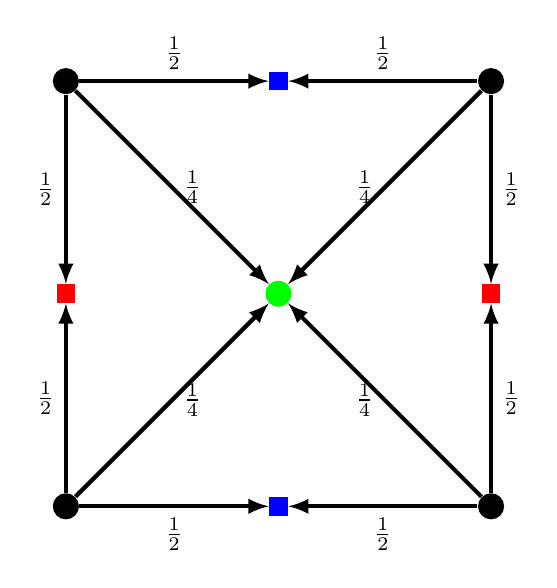
\begin{tikzpicture}[scale=0.9]
        % Define os nos
        \node[circle,fill=black] (A) at (0,6) {};
        \node[circle,fill=black] (B) at (6,6) {};
        \node[circle,fill=black] (C) at (6,0) {};
        \node[circle,fill=black] (D) at (0,0) {};
        \node[rectangle,fill=blue] (E) at (3,6) {};
        \node[rectangle,fill=blue] (F) at (3,0) {};
        \node[rectangle,fill=red] (G) at (0,3) {};
        \node[rectangle,fill=red] (H) at (6,3) {};
        \node[circle,fill=green] (I) at (3,3) {};
        % Conecta nos
        \draw[->, thick, >=latex, line width=1.5pt] (A) -- node[above] {$\frac{1}{2}$} (E);
        \draw[->, thick, >=latex, line width=1.5pt] (B) -- node[above] {$\frac{1}{2}$} (E);
        \draw[->, thick, >=latex, line width=1.5pt] (B) -- node[right] {$\frac{1}{2}$} (H);
        \draw[->, thick, >=latex, line width=1.5pt] (C) -- node[right] {$\frac{1}{2}$} (H);
        \draw[->, thick, >=latex, line width=1.5pt] (C) -- node[below] {$\frac{1}{2}$} (F);
        \draw[->, thick, >=latex, line width=1.5pt] (D) -- node[below] {$\frac{1}{2}$} (F);
        \draw[->, thick, >=latex, line width=1.5pt] (D) -- node[left]  {$\frac{1}{2}$} (G);
        \draw[->, thick, >=latex, line width=1.5pt] (A) -- node[left]  {$\frac{1}{2}$} (G);
        \draw[->, thick, >=latex, line width=1.5pt] (A) -- node[right] {$\frac{1}{4}$} (I);
        \draw[->, thick, >=latex, line width=1.5pt] (B) -- node[left]  {$\frac{1}{4}$} (I);
        \draw[->, thick, >=latex, line width=1.5pt] (C) -- node[left]  {$\frac{1}{4}$} (I);
        \draw[->, thick, >=latex, line width=1.5pt] (D) -- node[right] {$\frac{1}{4}$} (I);
    \end{tikzpicture}
    \fadaptada{rogenski2011desenvolvimento}
\end{figure}

Na malha $4h$, realiza-se mais uma série de $N_3$ iterações utilizando o método de Gauss-Seidel, resolvendo a equação:
\[
\nabla^2 v_{4h} = s_{4h}.
\]
O ciclo multigrid é finalizado após aplicar uma nova interpolação bilinear e corrigir os valores na malha $2h$, como mostrado na \autoref{fig_multigrid_cicle_v}. O número de ciclos repetidos depende da tolerância de erro especificada para o resíduo final na malha refinada. O algoritmo continua até que o erro residual seja inferior ao valor de tolerância definido.

\begin{figure}[htb]
    \centering
    \caption{Esquema do ciclo V no método multigrid FAS.}\label{fig_multigrid_cicle_v}
    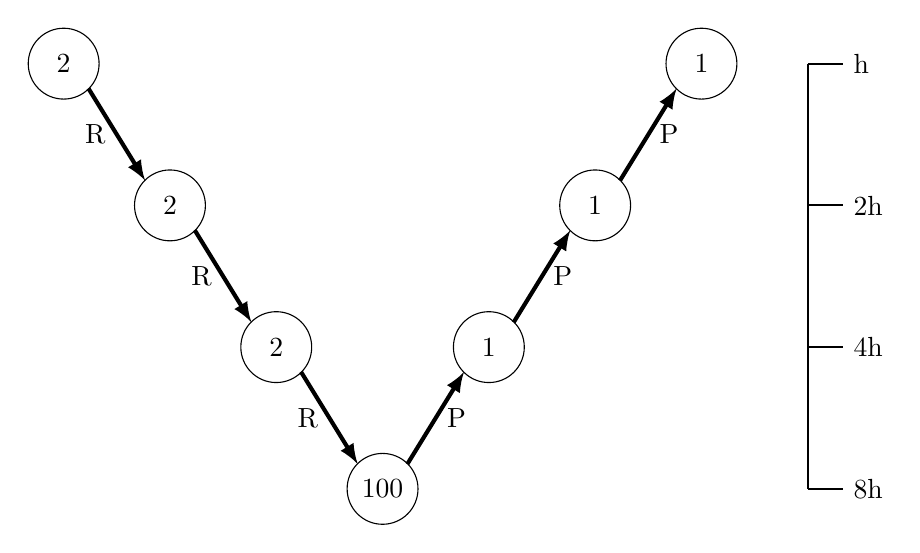
\begin{tikzpicture}[scale=0.9]
        \draw (0,8) circle (0.5) node {2};
        \draw (1.5,6) circle (0.5) node {2};
        \draw (3,4) circle (0.5) node {2};
        \draw (4.5,2) circle (0.5) node {100};
        \draw (6,4) circle (0.5) node {1};
        \draw (7.5,6) circle (0.5) node {1};
        \draw (9,8) circle (0.5) node {1};
        \draw[->, thick, >=latex, line width=1.5pt] (0.35,7.65) -- (1.15,6.35) node[midway,left] {R};
        \draw[->, thick, >=latex, line width=1.5pt] (1.85,5.65) -- (2.65,4.35) node[midway,left] {R};
        \draw[->, thick, >=latex, line width=1.5pt] (3.35,3.65) -- (4.15,2.35) node[midway,left] {R};
        \draw[->, thick, >=latex, line width=1.5pt] (7.85,6.35) -- (8.65,7.65) node[midway,right] {P};
        \draw[->, thick, >=latex, line width=1.5pt] (6.35,4.35) -- (7.15,5.65) node[midway,right] {P};
        \draw[->, thick, >=latex, line width=1.5pt] (4.85,2.35) -- (5.65,3.65) node[midway,right] {P};
        \draw[thick] (10.5,8) -- (10.5,2);
        \draw[thick] (10.5,8) -- (11,8) node[right] {h};
        \draw[thick] (10.5,6) -- (11,6) node[right] {2h};
        \draw[thick] (10.5,4) -- (11,4) node[right] {4h};
        \draw[thick] (10.5,2) -- (11,2) node[right] {8h};
    \end{tikzpicture}
    \fadaptada{rogenski2011desenvolvimento}
\end{figure}

O método multigrid destaca-se por sua eficácia em acelerar a convergência de soluções numéricas para equações diferenciais parciais, especialmente em problemas elípticos, como a equação de Poisson. A abordagem multiescala, que combina malhas refinadas e grosseiras, permite corrigir os erros em diferentes escalas, resultando em uma solução rápida e precisa.

Para todos os casos considerados, $N_3=1$. O número de ciclos necessário para que a solução da equação seja, de fato, obtida, está associado ao resíduo obtido na malha mais fina. Se o valor obtido for menor do que uma dada tolerância de referência, o algoritmo é finalizado.

\section{Método de filtragem}\label{SecFiltragem}

Adotou-se também a estratégia de se realizar filtragem espacial baseada em \cite{lele1992compact}. Dentre os diversos métodos compactos de filtragem propostos pelo autor, opta-se pelo uso de um método compacto tridiagonal de até sexta ordem de precisão. A filtragem é aplicada ao final de cada iteração temporal e consiste em recalcular a distribuição dos componentes de vorticidade por meio de um sistema, no caso:
\begin{align}
\left[\begin{array}{ccccccccccc}
1 &  & & & & & & & & &\\
 & 1 &  & & & & & & & & \\
& & 1 & & & & & & & &\\
& &  & . & . & .&  &  & & & \\
& & &  & \alpha & 1 & \alpha &  & & &  \\
& & & &  & . & . & . &  & & \\
& & & & &  &  & & 1 & & \\
& & & & &  &  & & & 1 & \\
& & & & &  &  & & &  & 1
\end{array}\right] \left[\begin{array}{c}
\varphi_{z1} \\
\varphi_{z2}  \\
\varphi_{z3}  \\
 . \\
\varphi_{zi}  \\
 . \\
\varphi_{zimax-2} \\
\varphi_{zimax-1} \\
\varphi_{zimax} 
\end{array}\right] = \hspace{1cm} \nonumber\\ 
=\left[\begin{array}{c}
(15\varphi_{z1}^* +  4 \varphi_{z2}^* -  6 \varphi_{z3}^* +  4  \varphi_{z4}^*
 -         \varphi_{z5}^* ) / 16 \\
( \varphi_{z1}^* + 12\varphi_{z2}^*+  6\varphi_{z3}^* -  4 \varphi_{z4}^*
+         \varphi_{z5}^*) / 16\\
 (   - \varphi_{z1}^* +  4\varphi_{z2}^*
+ 10\varphi_{z3}^* +  4\varphi_{z4}^* - \varphi_{z5}^* ) / 16\\
. \\
\begin{gathered}
af \varphi_{z_i}^*+bf\left[\varphi_{z_{i+1}^*}+\varphi_{z_{i-1}^*}\right]+ \\
cf\left[\varphi_{z_{i+2}^*}+\varphi_{z_{i-2}^*}\right]+df\left[\varphi_{z_{i+3}^*}+\varphi_{z_{i-3}^*}\right]
\end{gathered} \\
. \\
( - \varphi_{zimax}^* +  4\varphi_{zimax-1}^* + 10\varphi_{zimax-2}^* +  4\varphi_{zimax-3}^* - \varphi_{zimax-4}^* ) / 16  \\
(\varphi_{zimax}^* + 12\varphi_{zimax-1}^* +  6\varphi_{zimax-2}^* -  4 \varphi_{zimax-3}^* + \varphi_{zimax-4}^*) / 16 \\
(15\varphi_{zimax}^* +  4\varphi_{zimax-1}^* -  6 \varphi_{zimax-2}^* +  4  \varphi_{zimax-3}^* -  \varphi_{zimax-4}^*)/16 \end{array}\right],\label{filtragem_espacial}
\end{align}
em que $\varphi^*$ representa a $\varphi$ antes da aplicação do filtro computacional. Define-se também as constantes $af=(11+10\alpha)/16$, $bf=(15+34\alpha)/64$, $cf=(-3+6\alpha)/32$ e $df=(1-2\alpha)/64$ segundo \citeonline{lele1992compact}. O valor do $\alpha$ é escolhido de acordo com a faixa de frequências que se deseja filtrar.

\section{Cálculo das condições de contorno}

Nas paredes do domínio, foram impostas condições de contorno de não deslizamento e impermeabilidade, exceto na tampa superior, onde foi simulada uma condição semelhante ao problema da cavidade. Nesse cenário, a velocidade horizontal é dada por $ u = \varphi(x) $ e a velocidade vertical é nula ($ v = 0 $) em $ y = 1 $, enquanto nas outras fronteiras $ u = v = 0 $.

Na formulação Vorticidade-Função de Corrente, conforme apresentado por \citeonline{roache1972computational}, o cálculo da vorticidade é realizado após a determinação da função corrente $ \psi $. Utilizam-se aproximações de quarta ordem para obter maior precisão nas derivadas, conforme mostrado nas equações \eqref{parede_baixo_vortici} a \eqref{parede_direita_vortici}:

\begin{align}
    \omega_{i,1} &= \frac{-85\psi_{i,1} + 108\psi_{i,2} - 27\psi_{i,3} + 4\psi_{i,4}}{18dy^{2}} + O(h^{4}), \label{parede_baixo_vortici} \\
    \omega_{i,jmax} &= \frac{11u_{i,jmax} - 18u_{i,jmax-1} + 9u_{i,jmax-2} - 2u_{i,jmax-3}}{6dy} + O(h^{4}), \label{parede_cima_vortici}\\
    \omega_{1,j} &= \frac{-85\psi_{1,j} + 108\psi_{2,j} - 27\psi_{3,j} + 4\psi_{4,j}}{18dy^{2}} + O(h^{4}), \label{parede_esquerda_vortici}\\
    \omega_{imax,j} &= \frac{-85\psi_{imax,j} + 108\psi_{imax-1,j} - 27\psi_{imax-2,j} + 4\psi_{imax-3,j}}{18dy^{2}} + O(h^{4}). \label{parede_direita_vortici}
\end{align}

As equações \eqref{parede_baixo_vortici} e \eqref{parede_cima_vortici} foram aplicadas para as condições de contorno em $ y = 0 $ e $ y = 1 $, respectivamente, para $ i = 2, \dots, imax-1 $. Já as equações \eqref{parede_esquerda_vortici} e \eqref{parede_direita_vortici} foram empregadas para as fronteiras em $ x = 0 $ e $ x = 1 $, para $ j = 2, \dots, jmax-1 $. Essas aproximações garantem que as condições de contorno físicas do problema sejam mantidas, assegurando uma solução precisa tanto para a vorticidade quanto para a função corrente em escoamentos viscoelásticos.

No caso específico dos tensores de tensão polimérica, as condições de contorno foram impostas a partir de uma solução manufaturada construída previamente. Essa abordagem permite controlar precisamente os campos de velocidade, pressão e tensões, facilitando a verificação do método numérico. Ao aplicar valores analíticos conhecidos nas fronteiras, é possível avaliar de forma rigorosa a exatidão da implementação e dos esquemas diferenciais empregados no interior do domínio. Essa técnica é amplamente utilizada em estudos de validação e benchmark de códigos numéricos.
% ---------------------------------------------------------------------------
% ---------------------------------------------------------------------------
% Capítulo 4 - MMS
% ---------------------------------------------------------------------------
% ----------------------------------------------------------
%% Capitulo4-MetodosSolucoesManufaturadas.tex 
% ----------------------------------------------------------
% Metodos Numericos
% ----------------------------------------------------------
\chapter[MMS]{Métodos das Soluções Manufaturadas}
\label{Cap_MetodosSolucoesManufaturadas}

A abordagem adotada para a aplicação do Método de Soluções Manufaturadas (MMS) seguiu os princípios descritos por \citeonline{shih1989effects}, sendo um método amplamente utilizado no campo das simulações numéricas e da modelagem computacional \cite{Roy2004, Roy2001, Roache2002}. A relevância do MMS reside em sua capacidade de criar um ambiente controlado para a verificação de códigos numéricos, onde geralmente não se possui uma solução para o problema ao qual o código se destina. Ao gerar soluções exatas ou analíticas com características previamente conhecidas, torna-se possível avaliar a precisão, a convergência e a estabilidade dos métodos numéricos empregados. Além disso, o MMS permite que se examine a fidelidade desses métodos em diferentes condições, garantindo sua robustez em uma ampla gama de cenários. Esse método também facilita a identificação e correção de artefatos numéricos que possam comprometer a qualidade dos resultados das simulações.

\section{Geração de soluções manufaturadas}\label{Sec_geracao_solucoes_manufaturadas}

A geração de soluções manufaturada consiste, essencialmente, na introdução de um termo fonte nas equações governantes. Esse termo fonte é especialmente construído para forçar uma solução analítica a um problema semelhante ao inicial proposto, porém previamente determinada. Para gerar as soluções manufaturadas, adotou-se a notação $\overline{f}$ para representar as funções pré-definidas ou impostas, enquanto $\widetilde{f}$ denota aquelas funções que são derivadas das equações governantes. Inicialmente, define-se as funções previamente conhecidas, como $\overline{u}$, $\overline{T}_{xx}$, $\overline{T}_{xy}$ e $\overline{T}_{yy}$. Assim considerando $\overline{u}$ como uma função conhecida, e utilizando a \autoref{eq_cont_bidime} pode-se obter $\widetilde{v}$ fazendo:
\begin{gather}
    \widetilde{v} = - \int \frac{\partial \overline{u}}{\partial x}dy.\label{eq_MMS_v_linha}
\end{gather}

Utilizando $\overline{u}$ e $\widetilde{v}$, pode-se obter $\widetilde{\omega_z}$ fazendo:
\begin{align}\label{eq_vortic_wz}
    \widetilde{\omega_z} = \frac{\partial \overline{u}}{\partial y}-\frac{\partial \widetilde{v}}{\partial x}
\end{align}
e $\widetilde{\Psi}$ resolvendo:
\begin{align}\label{eq_funcaocorrente_psi}
    \frac{\partial \Psi}{\partial y} = \overline{u}\quad\text{ ou }\quad\frac{\partial \Psi}{\partial x} = -\overline{v}.
\end{align}

Com $\overline{u}$ estabelecida e $\widetilde{v}$ e $\widetilde{\omega_z}$ obtidas por meio das Equações \eqref{eq_MMS_v_linha} e \eqref{eq_vortic_wz}, e considerando ainda as funções $\overline{T^{xx}}$, $\overline{T^{xy}}$ e $\overline{T^{yy}}$ também conhecidas, substitui-se essas funções nas Equações \eqref{eq_movi_x_bidime},\eqref{eq_movi_y_bidime},\eqref{eq_lpog_txx},\eqref{eq_lpog_txy} e \eqref{eq_lpog_tyy}, fazendo com que seja necessário acrescentar os termos fontes, como apresentado nas Equações \eqref{eq_vortic_corrent_MMS}, \eqref{eq_lpog_txx_source_term_1}, \eqref{eq_lpog_txy_source_term_1} e \eqref{eq_lpog_tyy_source_term_1}:
\begin{gather}
    \begin{aligned}
        \frac{\partial \omega_{z}}{\partial t} + \frac{\partial (u\omega_{z})}{\partial x} + \frac{\partial (v\omega_{z})}{\partial y} = \frac{\beta_{nn}}{Re}\left(\frac{\partial^{2} \omega_{z}}{\partial x^{2}} + \frac{\partial^{2} \omega_{z}}{\partial y^{2}}\right) + \frac{\partial^{2}T_{xx}}{\partial x^{}\partial y^{}} & +  \frac{\partial^{2}T_{xy}}{\partial y^{2}} - \frac{\partial^{2}T_{xy}}{\partial x^{2}} - \\ & -  \frac{\partial^{2}T_{yy}}{\partial x^{}\partial y^{}} + tf\omega_{z},
    \end{aligned}
    \label{eq_vortic_corrent_MMS}
\end{gather}
\begin{gather}
    \begin{aligned}
        f(\mathbf{T})T_{xx} & + Wi\bigg[\frac{\partial T_{xx}}{\partial t} + \frac{\partial (uT_{xx})}{\partial x} + \frac{\partial (vT_{xx})}{\partial y} - 2T_{xx}\frac{\partial u}{\partial x} - 2T_{xy}\frac{\partial u}{\partial y}\bigg] + \frac{\alpha_{G}\operatorname{Wi}\operatorname{Re}}{1-\beta_{nn}}\left(T_{xx}^{2} + T_{xy}^{2}\right) + \\ & + \xi\operatorname{Wi}\left(2T_{xx}\frac{\partial u}{\partial x} + T_{xy}\left(\frac{\partial u}{\partial y} + \frac{\partial v}{\partial x}\right)\right) = 2\frac{1-\beta_{nn}}{\operatorname{Re}}\frac{\partial u}{\partial x} + tfT_{xx},
    \end{aligned}
    \label{eq_lpog_txx_source_term_1}
\end{gather}
\begin{gather}
    \begin{aligned}
        f(\mathbf{T})T_{xy} & + Wi\bigg[\frac{\partial T_{xy}}{\partial t} + \frac{\partial (uT_{xy})} {\partial x} + \frac{\partial (vT_{xy})}{\partial y} - T_{xx}\frac{\partial v}{\partial x} - T_{yy}\frac{\partial u}{\partial y}\bigg] + \frac{\alpha_{G}\operatorname{Wi}\operatorname{Re}}{1-\beta_{nn}}\left[T_{xy}\left(T_{xx} + T_{yy}\right)\right] + \\ 
        & + \frac{\xi\operatorname{Wi}}{2}\left(T_{xx} + T_{yy}\right)\left(\frac{\partial u}{\partial y} + \frac{\partial v}{\partial x}\right) = \frac{1-\beta_{nn}}{\operatorname{Re}}\left(\frac{\partial v}{\partial x} + \frac{\partial u}{\partial y}\right)+ tfT_{xy},
    \end{aligned}
    \label{eq_lpog_txy_source_term_1}
\end{gather}
\begin{gather}
    \begin{aligned}
        f(\mathbf{T})T_{yy} &+ Wi\bigg[\frac{\partial T_{yy}}{\partial t} + \frac{\partial (uT_{yy})}{\partial x} + \frac{\partial (vT_{yy})}{\partial y} - 2T_{xy}\frac{\partial v}{\partial x} - 2T_{yy}\frac{\partial v}{\partial y}\bigg] + \frac{\alpha_{G}\operatorname{Wi}\operatorname{Re}}{1-\beta_{nn}}\left(T_{xy}^{2} + T_{yy}^{2}\right) + \\ & + \xi\operatorname{Wi}\left(2T_{yy}\frac{\partial v}{\partial y} + T_{xy}\left(\frac{\partial u}{\partial y} + \frac{\partial v}{\partial x}\right)\right) = 2\frac{1-\beta_{nn}}{\operatorname{Re}}\frac{\partial v}{\partial y}+ tfT_{yy},
    \end{aligned}
    \label{eq_lpog_tyy_source_term_1}
\end{gather}
onde os termos fontes são dados por:
\begin{gather}
    \begin{aligned}
        \mathbf{tf}\omega_{z} = & \frac{\partial \widetilde{\omega_{z}}}{\partial t} + \frac{\partial (\overline{u}\widetilde{\omega_{z}})}{\partial x} + \frac{\partial (\widetilde{v}\widetilde{\omega_{z}})}{\partial y} - \frac{\beta_{nn}}{Re}\left(\frac{\partial^{2} \widetilde{\omega_{z}}}{\partial x^{2}} + \frac{\partial^{2} \widetilde{\omega_{z}}}{\partial y^{2}}\right) \\ & - \frac{\partial^{2}\overline{T}_{xx}}{\partial x^{}\partial y^{}} - \frac{\partial^{2}\overline{T}_{xy}}{\partial y^{2}} + \frac{\partial^{2}\overline{T}_{xy}}{\partial x^{2}} + \frac{\partial^{2}\overline{T}_{yy}}{\partial x^{}\partial y^{}} ,
    \end{aligned}
    \label{eq_wz_s_t_2}
\end{gather}
\begin{equation}
    \begin{aligned}
        tfT_{xx} & = \overline{f}(\mathbf{T})\overline{T}_{xx} + \operatorname{Wi}\left[\frac{\partial \overline{T}_{xx}}{\partial t} + \frac{\partial (\overline{u}\overline{T}_{xx})}{\partial x} + \frac{\partial(\tilde{v}\overline{T}_{xx})}{\partial y} - 2\overline{T}_{xx}\frac{\partial \overline{u}}{\partial x} - 2\overline{T}_{xy}\frac{\partial \overline{u}}{\partial y}\right] + \\ & + \frac{\alpha_{G}\operatorname{Wi}\operatorname{Re}}{1-\beta_{nn}}\left(\overline{T}_{xx}^{2} - \overline{T}_{xy}^{2}\right) + \xi\operatorname{Wi}\left(2\overline{T}_{xx}\frac{\partial \overline{u}}{\partial x} + \overline{T}_{xy}\left(\frac{\partial \overline{u}}{\partial y} + \frac{\partial \tilde{v}}{\partial x}\right)\right) - 2\frac{1-\beta_{nn}}{\operatorname{Re}}\frac{\partial \overline{u}}{\partial x},
    \end{aligned}
    \label{eq_lpog_txx_s_t_2}
\end{equation}
\begin{equation}
    \begin{aligned}
        tfT_{xy} & = \overline{f}(\mathbf{T})\overline{T}_{xy} + \operatorname{Wi}\left[\frac{\partial \overline{T}_{xy}}{\partial t} + \frac{\partial (\overline{u}\overline{T}_{xy})} {\partial x} + \frac{\partial(\tilde{v}\overline{T}_{xy})}{\partial y} - \overline{T}_{xx}\frac{\partial\tilde{v}}{\partial x} - \overline{T}_{yy}\frac{\partial \overline{u}}{\partial y}\right] + \\ & + \frac{\alpha_{G}\operatorname{Wi}\operatorname{Re}}{1-\beta_{nn}}\left[\overline{T}_{xy}\left(\overline{T}_{xx} + \overline{T}_{yy}\right)\right] + \frac{\xi\operatorname{Wi}}{2}\left(\overline{T}_{xx} + \overline{T}_{yy}\right)\left(\frac{\partial \overline{u}}{\partial y} + \frac{\partial \tilde{v}}{\partial x}\right) - \frac{1-\beta_{nn}}{\operatorname{Re}}\left(\frac{\partial \tilde{v}}{\partial x} + \frac{\partial \overline{u}}{\partial y}\right),
    \end{aligned}
    \label{eq_lpog_txy_s_t_2}
\end{equation}
\begin{equation}
    \begin{aligned}
        tfT_{yy} & = \overline{f}(\mathbf{T})\overline{T}_{yy} + \operatorname{Wi}\left[\frac{\partial \overline{T}_{yy}}{\partial t} + \frac{\partial (\overline{u}\overline{T}_{yy})}{\partial x} + \frac{\partial (\tilde{v}\overline{T}_{yy})}{\partial y} - 2\overline{T}_{xy}\frac{\partial \tilde{v}}{\partial x} - 2\overline{T}_{yy}\frac{\partial \tilde{v}}{\partial y}\right] + \\ & + \frac{\alpha_{G}\operatorname{Wi}\operatorname{Re}}{1-\beta_{nn}}\left(\overline{T}_{xy}^{2} + \overline{T}_{yy}^{2}\right) + \xi\operatorname{Wi}\left(2\overline{T}_{yy}\frac{\partial\tilde{v}}{\partial y} + \overline{T}_{xy}\left(\frac{\partial \overline{u}}{\partial y} + \frac{\partial\tilde{v}}{\partial x}\right)\right) - 2\frac{1-\beta_{nn}}{\operatorname{Re}}\frac{\partial\tilde{v}}{\partial y},
    \end{aligned}
    \label{eq_lpog_tyy_s_t_2}
\end{equation}
com
\begin{equation}
    \begin{split}
        \overline{f}(\mathbf{T}) = \left( 1+\frac{\epsilon \operatorname{Wi} \operatorname{Re}}{(1 - \beta_{nm})}\right) \left(\overline{T}_{xx} + \overline{T}_{yy}\right).
    \end{split}\label{eq_funcao_traco_tensor_bidime_manufaturada}
\end{equation}

Um fato importante a ser observado é que a equação de Poisson não possui termo fonte justamente pela construção das soluções $\overline{u}$, $\widetilde{v}$ e $\widetilde{\omega}_{z}$.

\section{Solução manufaturada para testar métodos numéricos de alta ordem}

Para garantir a precisão na análise da ordem de convergência de códigos de alta ordem é preciso que as soluções manufaturadas evitem polinômios de ordem menor ou igual a ordem teórica dos métodos que são utilizados, pois o trucamento nas séries de Taylor que os métodos são baseados dariam zero e assim não seria possível verificar a ordem de convergência. Diante disso, propomos soluções baseadas em funções trigonométricas, como seno e cosseno, as quais permitem uma verificação detalhada da precisão dos métodos numéricos apresentados. Assim, as soluções manufaturadas propostas são dadas por:

\begin{gather}
    \begin{aligned}
        \overline{u}(x,y,t) &~= (x-1) x \sin(\pi x) \left(\sin(\pi y) + \pi y \cos(\pi y)\right) e^{-a\cdot t},\label{eq:u_case0}
    \end{aligned}
\end{gather}

Utilizando o procedimento descrito na ~\autoref{Sec_geracao_solucoes_manufaturadas}, obtemos:

\begin{gather}
    \begin{aligned}
        \widetilde{v}(x,y,t) &~= -y\sin(\pi y) \left((2x-1)\sin(\pi x) + \pi(x-1)x\cos(\pi x)\right)e^{-a\cdot t},\label{eq:v_case0}
    \end{aligned}
\end{gather}

\begin{gather}
    \begin{aligned}
        \widetilde{\omega_{z}}(x,y,t) = 2 &~ \bigg(\pi(x-1)x\sin(\pi x)\cos(\pi y) + y\sin(\pi y)\cdot \\ &~\cdot\left( (1 - \pi^2(x-1)x)\sin(\pi x) + \pi(2x-1)\cos(\pi x) \right)\bigg) e^{-a\cdot t},\label{eq:wz_case0}
    \end{aligned}
\end{gather}

\begin{gather}
    \begin{aligned}
        \widetilde{\psi}(x,y,t) &~= (x-1) x y \sin(\pi x)\sin(\pi y) e^{-a\cdot t}.\label{eq:psi_case0}
    \end{aligned}
\end{gather}

Por fim, para os tensores, consideramos as seguintes soluções manufaturadas:

\begin{gather}
    \begin{aligned}
        \overline{T}_{xx}(x,y,t) &~= (1-\beta_{nn})\left(\sin(\pi x) + \cos(\pi x) + 1\right) \left(\sin(\pi y) + \cos(\pi y) + 1\right)e^{-a\cdot t},\label{eq:txx_case0}
    \end{aligned}
\end{gather}

\begin{gather}
    \begin{aligned}
        \overline{T}_{xy}(x,y,t) &~= (1-\beta_{nn})\left(-\sin(\pi x) + \cos(\pi x) + 1\right) \left(-\sin(\pi y) + \cos(\pi y) + 1\right)e^{-a\cdot t},\label{eq:txy_case0}
    \end{aligned}
\end{gather}

\begin{gather}
    \begin{aligned}
        \overline{T}_{yy}(x,y,t) &~= (1-\beta_{nn})\left(\sin(\pi x) - \cos(\pi x) - 1\right) \left(\sin(\pi y) - \cos(\pi y) - 1\right)e^{-a\cdot t}.\label{eq:tyy_case0}
    \end{aligned}
\end{gather}

Para garantir uma comparação precisa dos resultados numéricos obtidos pelo código em teste, incluímos um fator multiplicativo de $(1-\beta_{nn})$ nas soluções manufaturadas dos tensores de tensão extra. Esse fator é essencial para ajustar os resultados em cenários envolvendo escoamentos Newtonianos, onde $\beta_{nn} = 1$. Nessas situações, o fator multiplicativo anula a contribuição dos tensores de tensão extra, fazendo com que a solução se alinhe com o comportamento de um fluido Newtoniano.

Por fim, os resultados completos das expressões analíticas correspondentes aos termos fonte associadas a Solução Manufaturada, aqui consideradas, são apresentadas no Anexo~\ref{chapter:fortran_77}, já em \textit{Fortran 77}. Além disso, no Anexo~\ref{chapter:mathematica_wolfran} apresentam-se os códigos para obtenção dessas expressões que foram obtidas via o \textit{ software Mathematica} para diferentes variáveis do escoamento, incluindo velocidades, vorticidade, função de corrente e tensores de tensão extra. Além disso, todos os códigos computacionais utilizados na geração desses termos fonte foram disponibilizados publicamente em um repositório no GitHub.
% ---------------------------------------------------------------------------
% Capítulo 5 - Resultados
% ---------------------------------------------------------------------------
% ----------------------------------------------------------
%% Capitulo5Resultados.tex
% ----------------------------------------------------------
% Resultados Numericos
% ----------------------------------------------------------
\chapter[Resultados]{Resultados Numéricos}
\label{Cap_ResultadosNumericos}

Neste capítulo, apresentam-se os resultados numéricos obtidos para verificar a implementação do código com os métodos apresentados no Capítulo \ref{Cap_MetodosNumericos}. O objetivo principal desta análise é avaliar a ordem numérica dos métodos utilizados no código. Além disso, destacamos a relevância do MMS para escoamentos de fluidos viscoelásticos, conforme introduzido neste estudo, como uma ferramenta confiável para a verificação e validação de outros códigos dentro do mesmo domínio de pesquisa.

\section{\textit{Softwares} utilizados e estrutura do código}\label{sec_ResultadosNumericos_software}

Para determinar os termos fonte essenciais no âmbito do MMS, utilizamos as capacidades do \textit{software Mathematica} \cite{Mathematica}, desenvolvido pela \textit{Wolfram Research}, amplamente reconhecido por suas funcionalidades em álgebra computacional e cálculos simbólicos.

O código principal foi implementado em \textit{Fortran77} \cite{Fortran97}, linguagem escolhida por sua eficiência em simulações numéricas de alto desempenho. Os procedimentos de pós-processamento e análise gráfica dos resultados foram conduzidos no ambiente \textit{MatLab}, explorando suas ferramentas de visualização e análise de dados científicos. O código principal segue a seguinte sequência de execução dos métodos numéricos: A simulação começa com a definição das condições iniciais e de contorno para cada variável $\varphi$, além de especificar o erro máximo admissível, denotado como $Er_{\infty}$, que determina quando as condições de estado estacionário são atingidas. Em seguida, o algoritmo continua em etapas iterativas, desde que $t$ permaneça menor que $t_f$ ou até que o critério pré-definido $Er_{\varphi} \geq Er_{\infty}$ seja atendido. Em cada iteração, as seguintes operações são executadas, considerando que a variável $\varphi$ representa, para efeitos de simplicidade, as variáveis $\omega_{z}$, $T^{xx}$, $T^{xy}$ e $T^{yy}$ simultaneamente: 1) Calcular os quatro estágios do método de Runge-Kutta para $\varphi$ (\autoref{eq_rk_4order}); 2) Determinar $\Psi$ resolvendo a equação de Poisson; 3) Aplicar a filtragem espacial em $\varphi$ (Equação (\autoref{filtragem_espacial}); e 4) Calcular as componentes de velocidade $u$ e $v$ utilizando o campo $\Psi$ obtido (\autoref{eq_Psiy_u_Psix_v}). Posteriormente, avalia-se o erro relativo $Er_{\varphi}$ e ajusta-se o passo de tempo $dt$ conforme necessário. No \autoref{code_pseudo} apresenta-se o pseudocódigo do que foi descrito.
\begin{algorithm}
\caption{Código com Runge-Kutta de quarta ordem}\label{code_pseudo}
\begin{algorithmic}[1]
\Function{main}{par.nn}
  \State Condições iniciais e de contorno para $\varphi$;
  \State Defina o valor de $Er_{\infty}$; \Comment{Erro máximo a ser alcançado no estado estacionário}
  \While {$t \leq tf$}
    \For{i}{\ 1 até }{4} 
       \State Calcula o passo $i$ do Runge-Kutta para $\varphi$ \eqref{eq_rk_4order}
       \State Calcula $\Psi$, resolvendo a equação de Poisson usando o método Multigrid;
       \State Realiza a filtragem espacial descrita em \eqref{filtragem_espacial} para $\varphi$;
       \State Calcula $u$ e $v$, usando $\Psi$  \eqref{eq_Psiy_u_Psix_v};
       \State Calcula $\omega$ na parede utilizando \eqref{parede_baixo_vortici}-\eqref{parede_direita_vortici};
    \EndFor
    \State Calcular $Er_{\varphi} = \frac{||\varphi^{n+1} - \varphi^{n}||_{\infty}}{||\varphi^{n+1}||_{\infty}}$; \Comment{Erro relativo}
    \If {$Er_{\varphi} \leq Er_{\infty}$ \textbf{e} $t \geq 0.01$}
        \State Finalizar avanço temporal
    \EndIf
    \State $t \gets t + dt $; \Comment{Passo de tempo ou incremento de tempo}
  \EndWhile
  \State Calcula o erro entre a solução numérica e analítica para $\varphi$;
\EndFunction
\end{algorithmic}
\end{algorithm}

Na etapa final deste processo, as discrepâncias entre as soluções numéricas e analíticas para cada variável $\varphi$ são comparadas para conseguir determinar . Essa comparação é feita calculando a norma $k$ para o termo de erro $e$, definido como:
\begin{align}
    &\left \|e\right \|_{k}=\left(\Delta x_{i} \Delta y_{j} \sum_{i=1}^{N_{i}}\sum_{j=1}^{N_{j}} \left |e\right |_{i,j}^{k}\right)^{1/k}, \label{norm_k}
\end{align}
onde $\Delta x_{i}$ e $\Delta y_{j}$ representam o espaçamento da malha nas direções $x$ e $y$, enquanto $N_{i}$ e $N_{j}$ são o número total de pontos nas respectivas direções, e $e$ é a diferença entre a solução manufaturada e a solução numérica. Essa fórmula permite uma avaliação quantitativa eficaz dos erros em todo o domínio computacional. Para determinar a ordem de convergência numérica, representada por $p$, adotamos o procedimento descrito por \citeonline{leveque2007finite}, que se baseia na seguinte relação logarítmica entre os erros obtidos em sucessivas resoluções de malha:
\begin{equation}\label{log_p} 
    p \approx \frac{\log\left(\frac{e_{l}}{e_{l+1}}\right)}{\log\left(\frac{h_{l}}{h_{l+1}}\right)},
\end{equation}
onde $e_{l}$ é o erro associado a espaçamento de malha $h_{l} = \max\limits_{N_i,N_j}\{\Delta x_{i};\ \Delta y_{j}\}.$ Essa abordagem permite verificar a taxa de convergência do método numérico utilizado, avaliando a relação entre os erros de discretização nas diferentes refinamentos de malha, o que é essencial para garantir a confiabilidade e precisão do código.

\section{Domínio computacional e parâmetros para a verificação}

Para todos os casos teste, considera-se o domínio $\Omega = [0;L]\times[0;H] = [0;1]\times[0;1]$, conforme ilustrado na \autoref{fig:domain}.
\begin{figure}[H]
        \centering
	\caption{Domínio computacional}\label{fig:domain}
        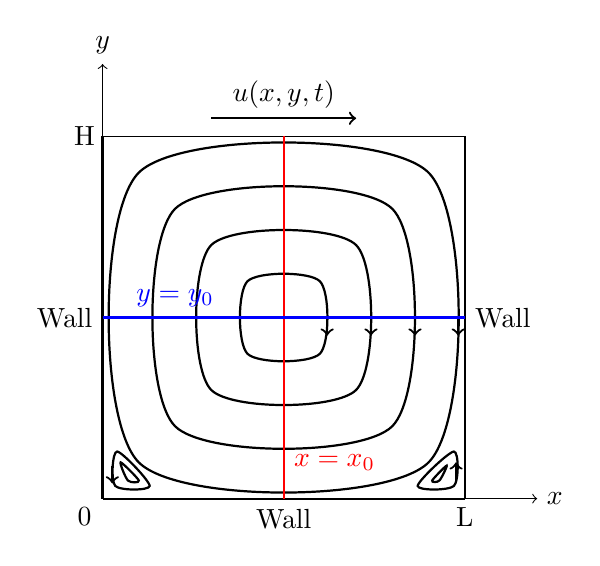
\begin{tikzpicture}[scale=4.6]
            % Eixos x e y
            \draw[->] (0,0) -- (1.2,0) node[right] {$x$};
            \draw[->] (0,0) -- (0,1.2) node[above] {$y$};
            % Desenhando o quadrado do domínio
            \draw (0,0) rectangle (1,1);
            % Desenho da tampa (lid)
            % \draw[->, thick] (0,1) -- (1,1) node[midway, above] {Lid};
            \draw[-, thick]  (0,0) -- (1,0) node[midway, below] {Wall};
            \draw[-, thick]  (0,0) -- (0,1) node[midway, left] {Wall};
            \draw[-, thick]  (1,0) -- (1,1) node[midway, right] {Wall};
            \draw[->, thick] (0.3,1.05) -- (0.7,1.05) node[midway, above] {$u(x,y,t)$};
            % Outras anotações
            \node at (-0.05,-0.05) {0};
            \node at (1,-0.05) {L};
            \node at (-0.05,1) {H};
            % Vortice central
            \draw[thick] plot[smooth cycle] coordinates {(0.1,0.9) (0.9,0.9) (0.9,0.1) (0.1,0.1)};
            \draw[thick] plot[smooth cycle] coordinates {(0.2,0.8) (0.8,0.8) (0.8,0.2) (0.2,0.2)};
            \draw[thick] plot[smooth cycle] coordinates {(0.3,0.7) (0.7,0.7) (0.7,0.3) (0.3,0.3)};
            \draw[thick] plot[smooth cycle] coordinates {(0.4,0.6) (0.6,0.6) (0.6,0.4) (0.4,0.4)};
            \draw[->, thick] (0.62,0.5) -- (0.62,0.45);
            \draw[->, thick] (0.741,0.5) -- (0.741,0.45);
            \draw[->, thick] (0.8625,0.5) -- (0.8625,0.45);
            \draw[->, thick] (0.982,0.5) -- (0.982,0.45);
            % Vortice inferrior esquerdo
            \draw[thick] plot[smooth cycle] coordinates {(0.07,0.05) (0.05,0.1) (0.1,0.05)};
            \draw[thick] plot[smooth cycle] coordinates {(0.035,0.035) (0.04,0.13) (0.13,0.035)};
            \draw[->, thick] (0.027,0.09) -- (0.027,0.042);
            % Vortice inferior direito
            \draw[thick] plot[smooth cycle] coordinates {(0.93,0.05) (0.95,0.091) (0.91,0.05)};
            \draw[thick] plot[smooth cycle] coordinates {(0.97,0.035) (0.97,0.13) (0.87,0.035)};
            \draw[->, thick] (0.976,0.05) -- (0.976,0.1);
            % Linha vertical em x = 0.5
            \draw[red, thick] (0.5, 0) -- (0.5, 1) node[pos=0.1, right] {$x = x_0$};
            % Linha horizontal em y = 0.5
            \draw[blue, thick] (0, 0.5) -- (1, 0.5) node[pos=0.2, above] {$y = y_0$};
        \end{tikzpicture}
	\fautor
\end{figure}

Por meio da utilização do Método das Soluções Manufaturadas (MMS), torna-se possível gerar uma solução de referência pré-definida, que pode ser comparada com a solução numérica obtida a partir do código computacional. Essa comparação não apenas fornece uma medida quantitativa da precisão numérica do código, mas também permite identificar possíveis discrepâncias ou desvios entre as previsões numéricas e a solução analítica conhecida. Tais desvios são quantificados pelo cálculo do erro padrão, utilizando a Equação~\eqref{norm_k} com $k = 2$, conforme descrito abaixo:
\begin{align} 
    &||e||_{2}=\left( \Delta x \Delta y \sum_{i=1}^{N_{1}}\sum_{j=1}^{N_{2}} \left |e\right |_{i,j}^{2}\right)^{1/2}.\label{norm_2}
\end{align}

A fim de avaliar o comportamento dos métodos numéricos aplicados às equações governantes para fluidos viscoelásticos, realizamos uma série de testes com diferentes modelos reológicos: UCM, Oldroyd-B, Giesekus e LPTT. Para cada um desses modelos, variamos os parâmetros relevantes, tais como o número de Reynolds ($Re$), o parâmetro $\beta_{nn}$, o número de Weissenberg ($Wi$), e, no caso dos modelos Giesekus e LPTT, o parâmetro $\alpha_G$, bem como os parâmetros adicionais $\epsilon$ e $\xi$, para os quais esses modelos são sensíveis.

Os valores desses parâmetros foram escolhidos de maneira a testar o desempenho do código numérico em uma ampla gama de condições de escoamento, desde regimes dominados por forças viscosas até aqueles com fortes efeitos elásticos. Além disso, os parâmetros $\alpha_G$, $\epsilon$ e $\xi$ foram incluídos nos modelos onde suas contribuições são significativas para capturar a complexidade do comportamento reológico. 

A Tabela \ref{tab_test_cases} resume os valores dos parâmetros usados nos casos de teste para cada modelo reológico. Essa diversidade de parâmetros foi selecionada para garantir que o método numérico seja avaliado sob diferentes cenários, verificando sua robustez e precisão em situações que incluem tanto fluidos Newtonianos quanto fluidos viscoelásticos complexos.

\begin{table}[H]
	\IBGEtab{
            \caption{Parâmetros utilizados para os testes realizados}
            \label{tab_test_cases}
        }{
            \begin{tabular}{c|cccccc}
                \toprule
                \textbf{Modelo} & $\operatorname{Re}$ & $\beta_{nn}$ & $\operatorname{Wi}$ & $\alpha_{G}$ & $\epsilon$ & $\xi$ \\ \midrule
                \textbf{UCM} & 1, 10, 100, 400 e 1000 & 0 & 1, 5 e 10 & 0 & 0 & 0 \\ \midrule
                \textbf{Oldroyd-B} & 1, 10, 100, 400 e 1000 & 0.1, 0.5, 0.9 e 1 & 1, 5 e 10 & 0 & 0 & 0 \\ \midrule
                \textbf{Giesekus} & 1, 10, 100, 400 e 1000 & 0.1, 0.5, 0.9 e 1 & 1, 5 e 10 & 0.1, 0.5 e 0.85 & 0 & 0 \\ \midrule
                \textbf{LPTT} & 1, 10, 100, 400 e 1000 & 0.1, 0.5, 0.9 e 1 & 1, 5 e 10 & 0 & 0.5 e 1 & 0.1 e 0.5 \\ \bottomrule
            \end{tabular}
        }{
		\fdadospesquisa
	}
\end{table}

Para garantir a estabilidade e a acurácia das simulações, foi adotado um passo de tempo fixo $\Delta t = 10^{-5}$, enquanto os critérios de convergência dos esquemas iterativos foram definidos com tolerância de erro de $10^{-6}$ para as variáveis principais, como função corrente, vorticidade e com as componentes do tensor de tensão. Esses valores foram escolhidos com base em testes preliminares que demonstraram bom compromisso entre precisão numérica e custo computacional.

As Figuras~\ref{U_m_u_sol_num_case1map2} e \ref{T_m_u_sol_num_case1map2} apresentam as soluções manufaturadas em regime de estado estacionário para os campos de velocidade, vorticidade, função de corrente e componentes do tensor de tensão. Essas visualizações permitem verificar qualitativamente as soluções analíticas utilizadas através do Método da Solução Manufaturada, fornecendo uma base gráfica que complementa a análise quantitativa dos erros, a serem realizadas nas seções a seguir, e permite confirmar a coerência dos padrões de escoamento e das distribuições de tensões com os resultados esperados para o problema físico modelado.

\begin{figure}[H]
        \centering
        \caption{Soluções manufaturadas no regime de estado estacionário para o campo de velocidades $(\overline{u},\tilde{v})$, vorticidade $(\tilde{\omega_{z}})$ e função de corrente $(\tilde{\psi})$, considerando $\beta_{nn}=0.1$ e $a = 0.05$ em $t=0.1$}
        \label{U_m_u_sol_num_case1map2}
        \begin{subfigure}[b]{.47\textwidth}
            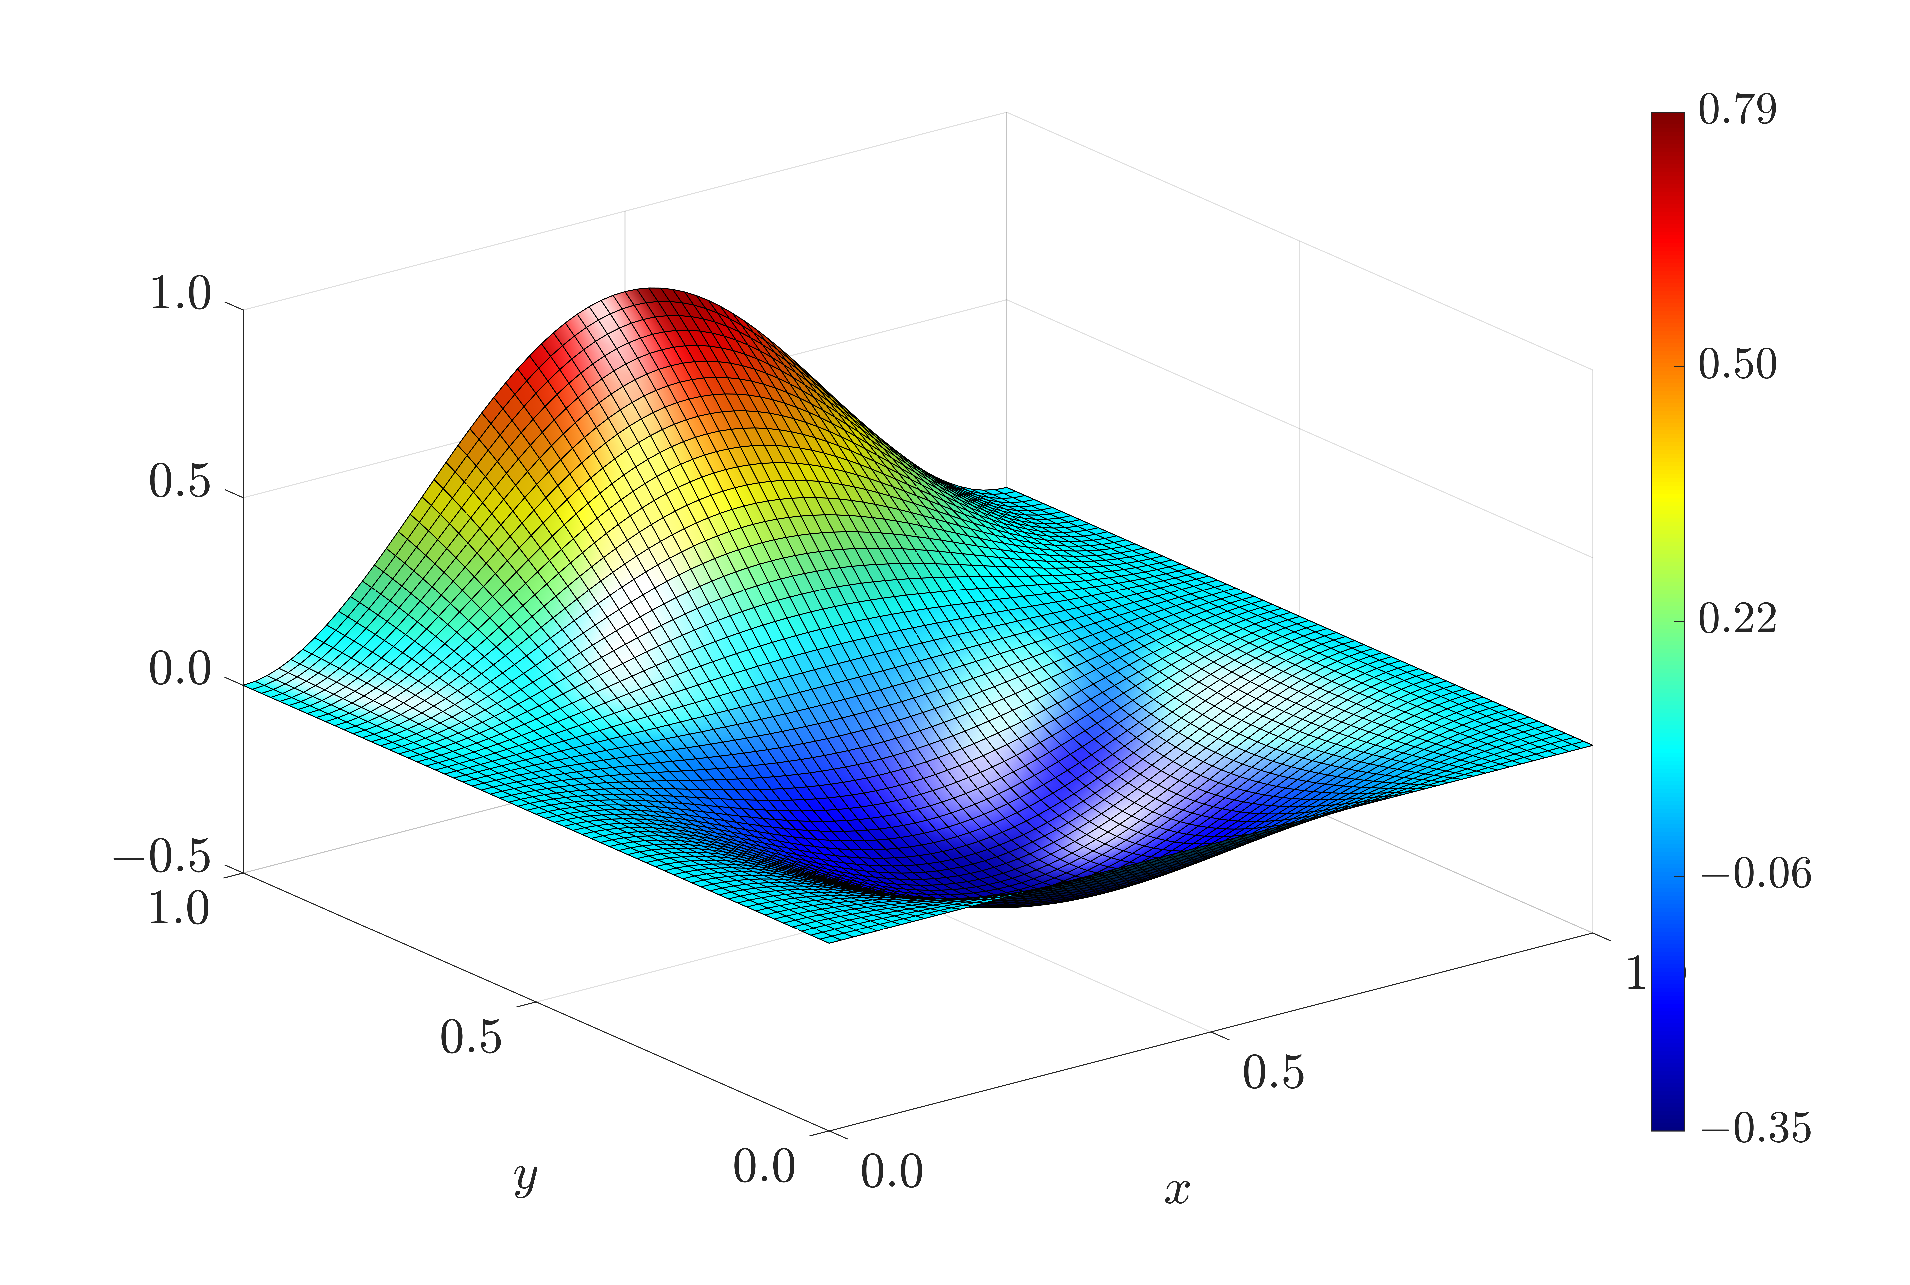
\includegraphics[width=\textwidth]{figures/Case12/UCM/Solutions/Exact_Surf_NormErr_2nd_Betann_0.1_Re_1_Wi_1_epsilon_0_xi_0_alphaG_0_Dt_1e-06_at_0.05_tipsim_1_MMS_12_U.eps}
            \caption{$\overline{u}$\label{fig_solexauCase1}}
        \end{subfigure}
        \vspace{0.2cm}
        \begin{subfigure}[b]{.47\textwidth}
            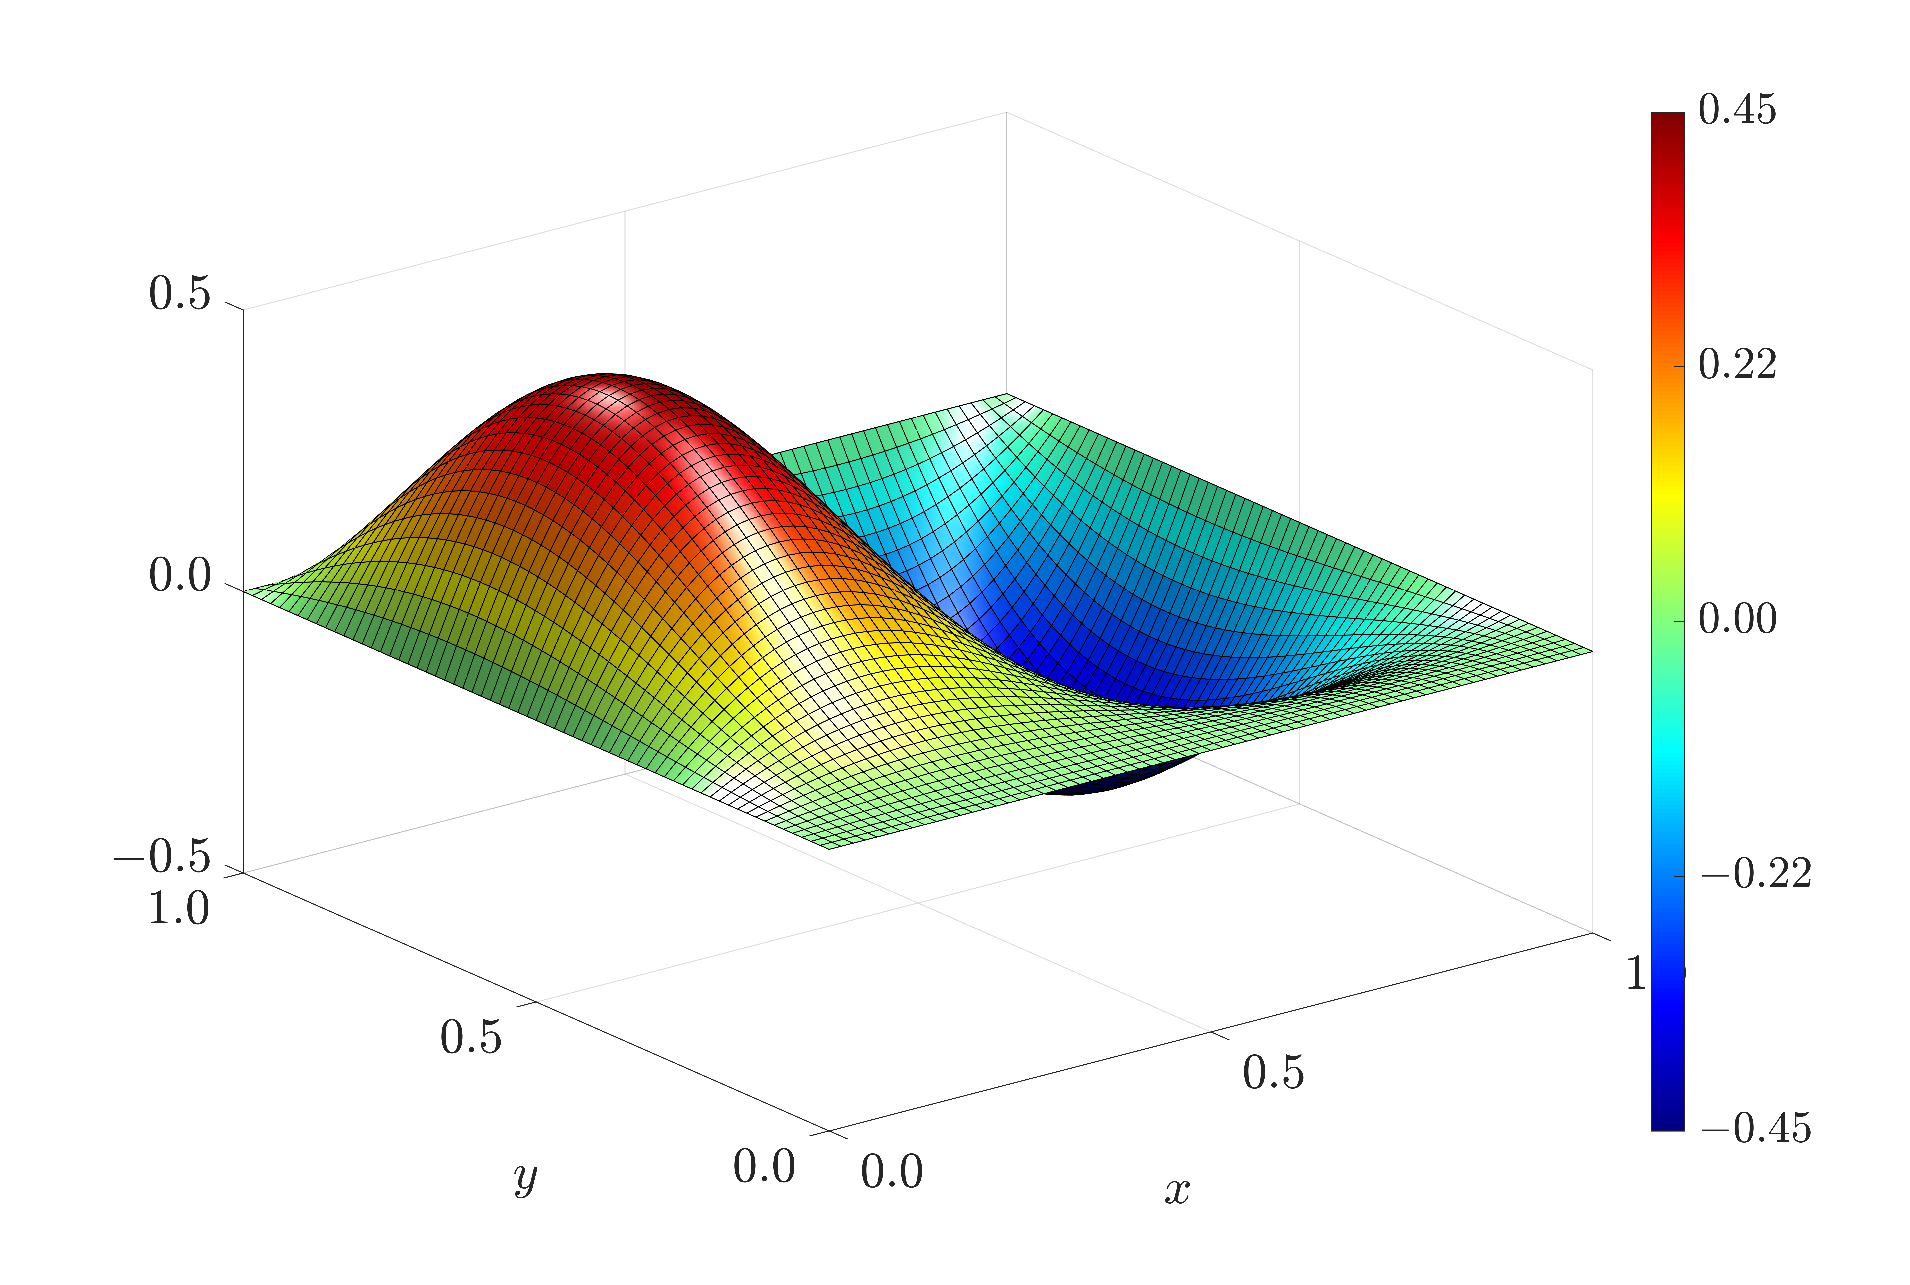
\includegraphics[width=\textwidth]{figures/Case12/UCM/Solutions/Exact_Surf_NormErr_2nd_Betann_0.1_Re_1_Wi_1_epsilon_0_xi_0_alphaG_0_Dt_1e-06_at_0.05_tipsim_1_MMS_12_V.eps}
            \caption{$\widetilde{v}$\label{fig_solexavCase1}}
        \end{subfigure}
        \begin{subfigure}[b]{.47\textwidth}
            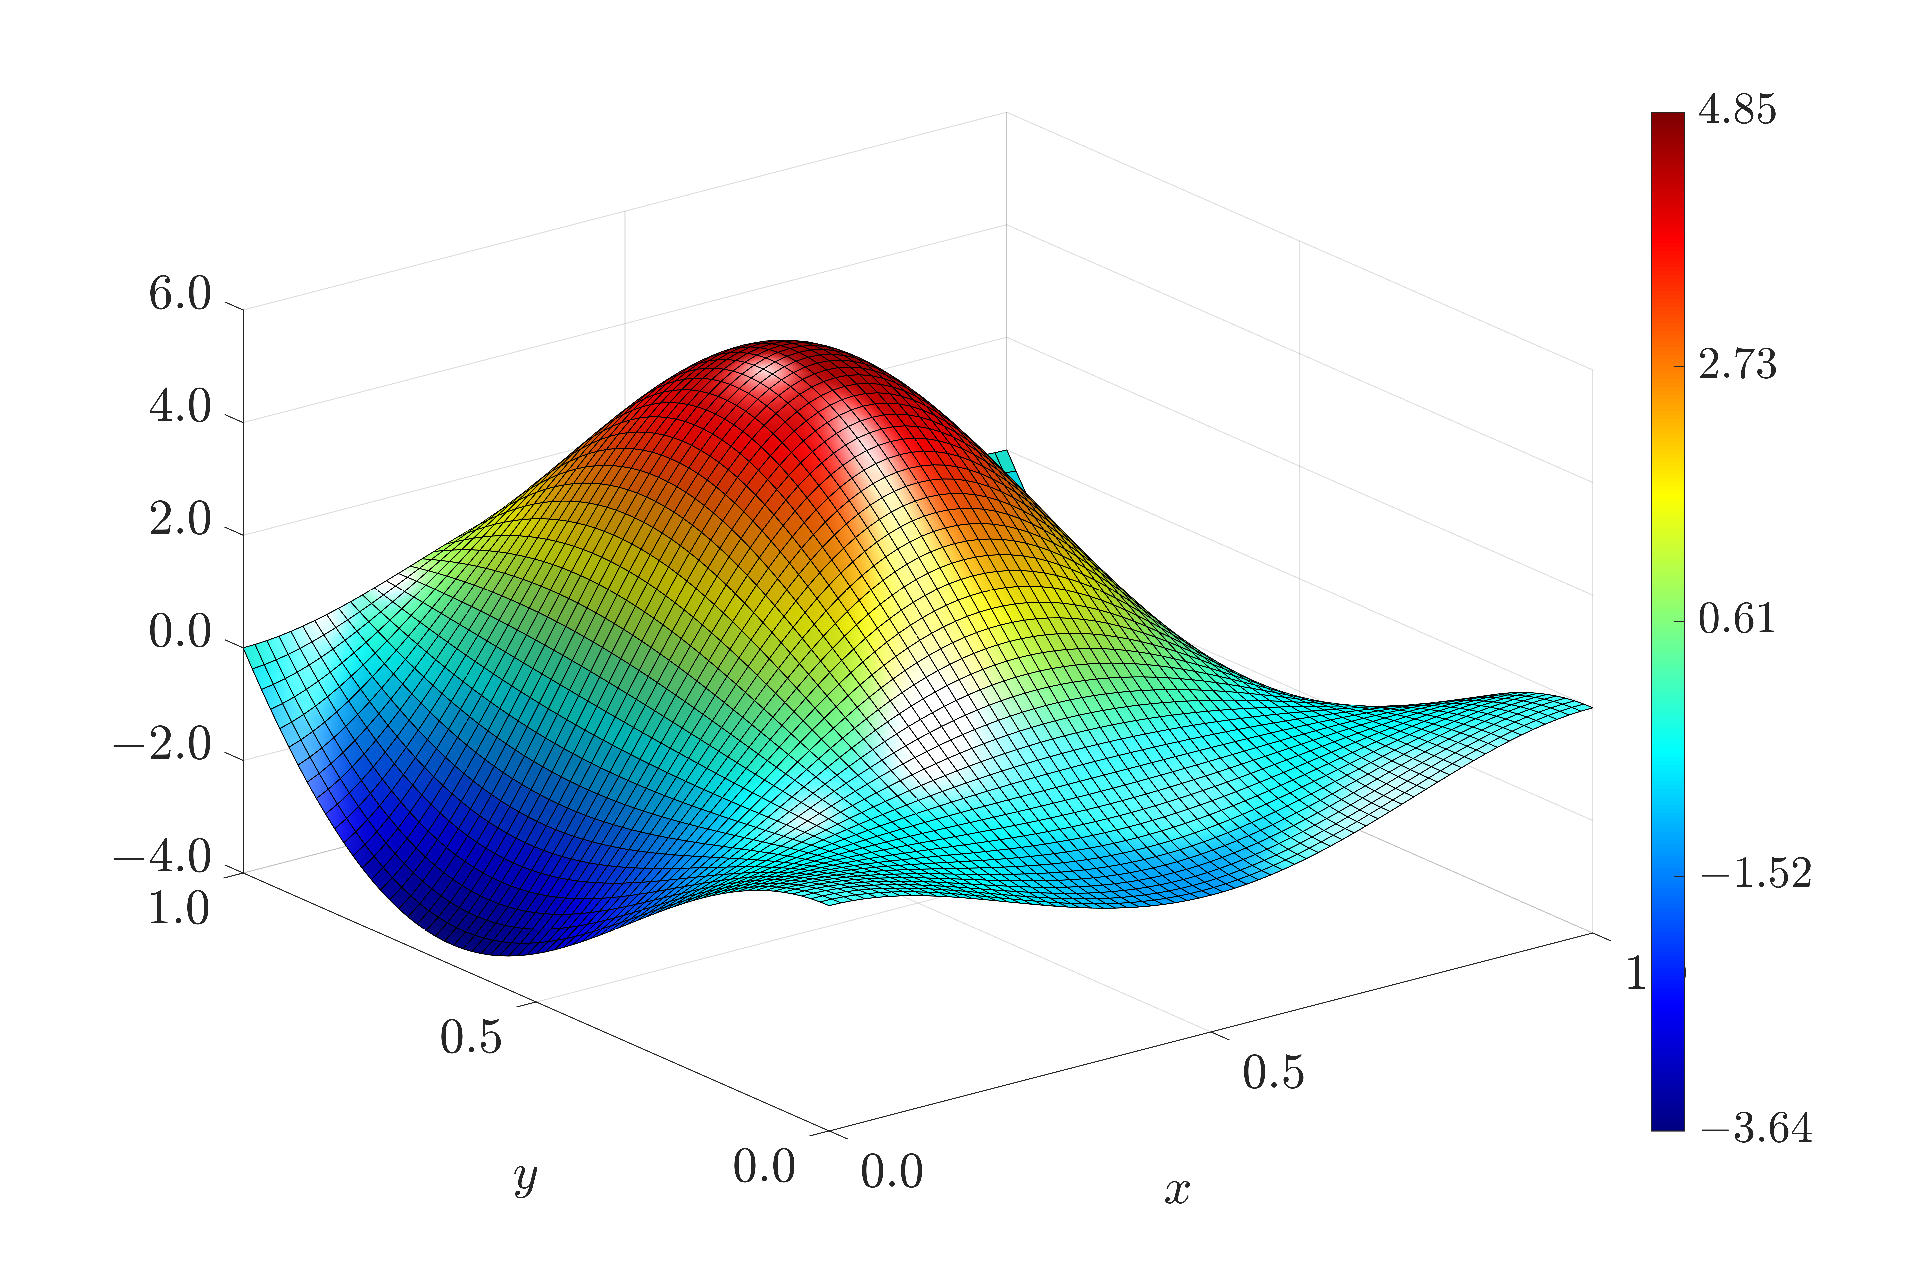
\includegraphics[width=\textwidth]{figures/Case12/UCM/Solutions/Exact_Surf_NormErr_2nd_Betann_0.1_Re_1_Wi_1_epsilon_0_xi_0_alphaG_0_Dt_1e-06_at_0.05_tipsim_1_MMS_12_Wz.eps}
            \caption{$\widetilde{\omega_{z}}$\label{fig_solexawzCase1}}
        \end{subfigure}
        \vspace{0.2cm}
        \begin{subfigure}[b]{.47\textwidth}
            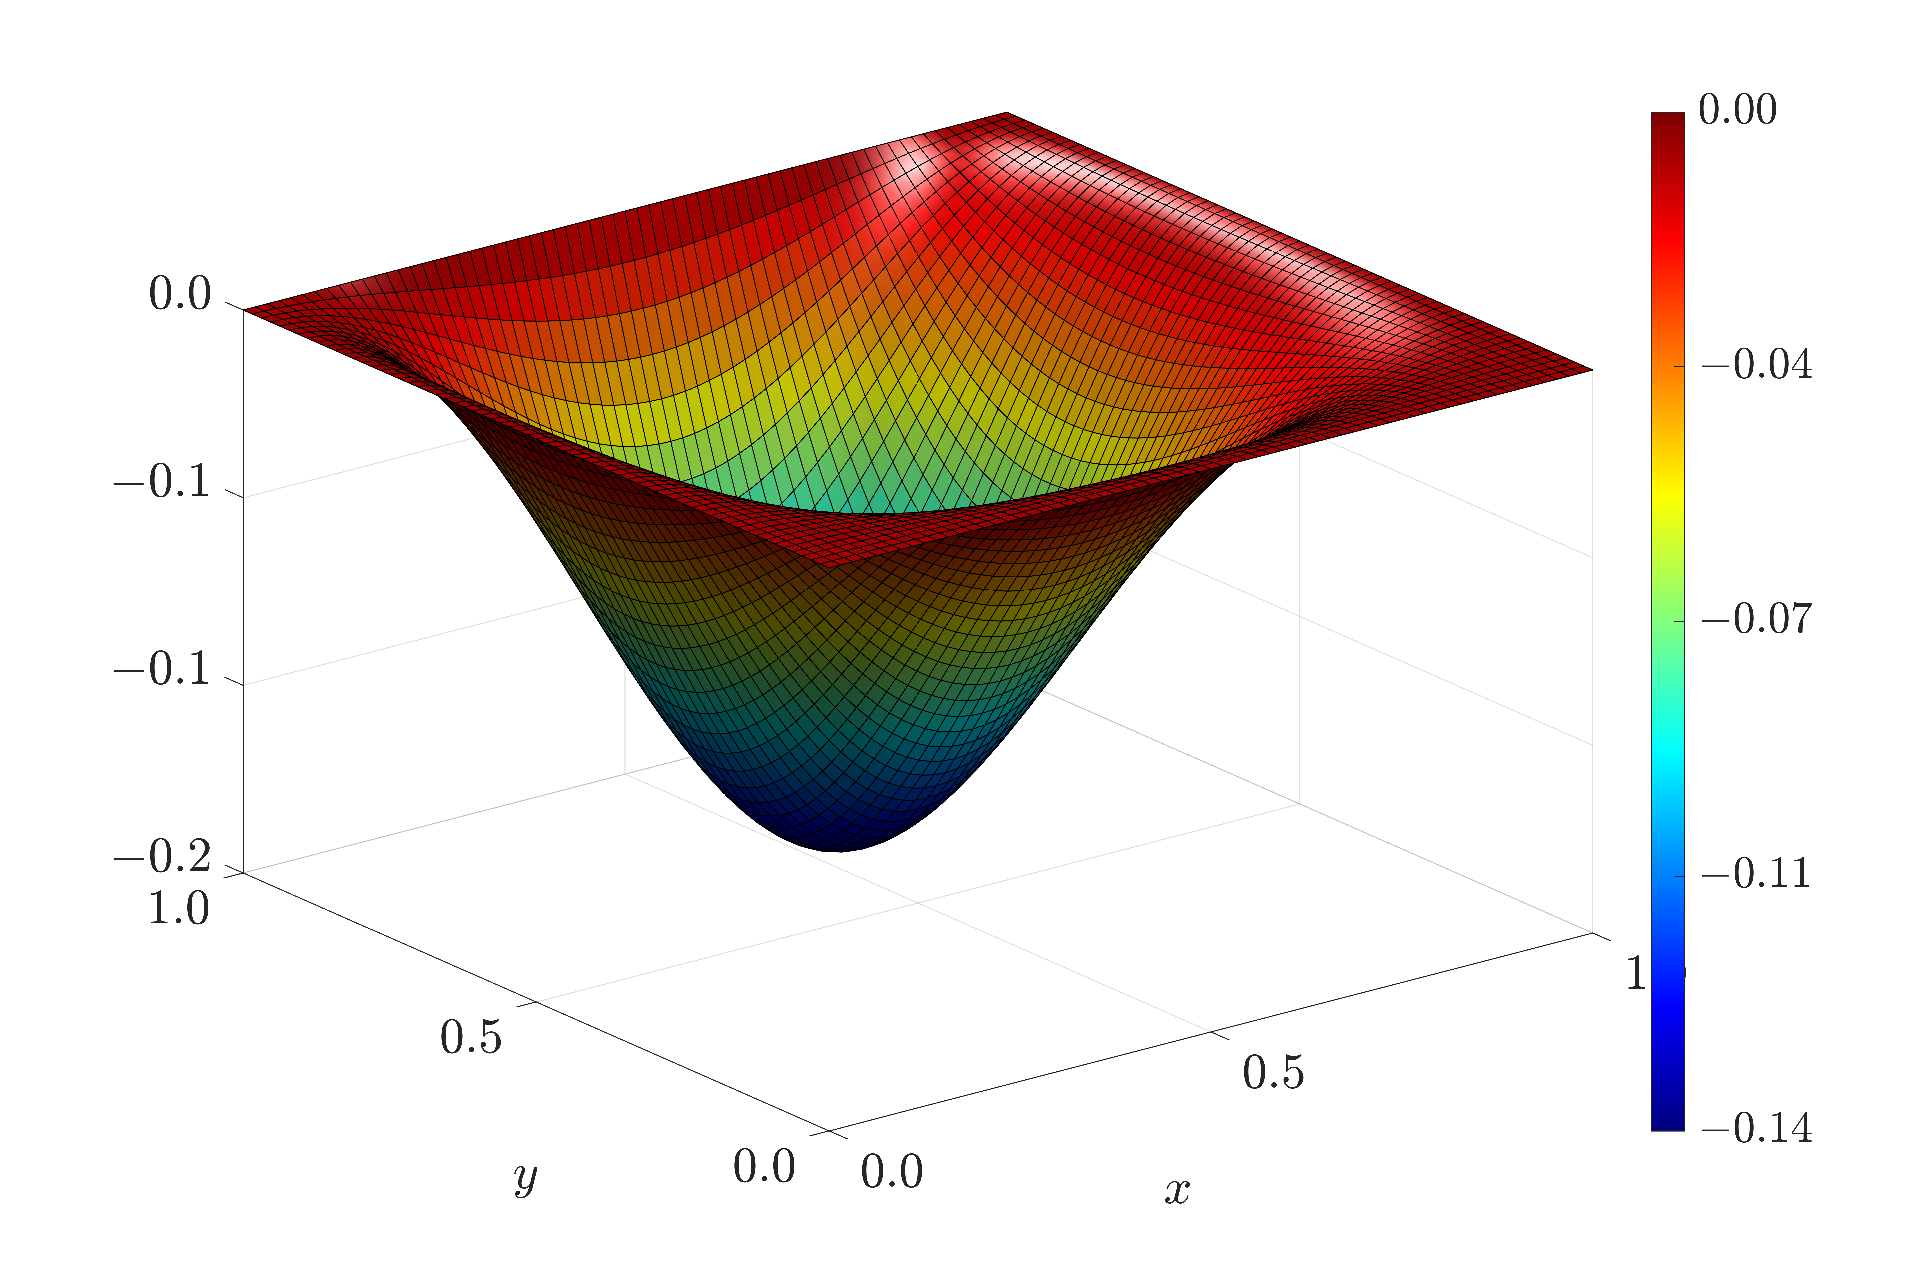
\includegraphics[width=\textwidth]{figures/Case12/UCM/Solutions/Exact_Surf_NormErr_2nd_Betann_0.1_Re_1_Wi_1_epsilon_0_xi_0_alphaG_0_Dt_1e-06_at_0.05_tipsim_1_MMS_12_Psi.eps}
            \caption{$\widetilde{\psi}$\label{fig_solexapsiCase1}}
        \end{subfigure}
        \fdadospesquisa
\end{figure}

\begin{figure}[H]
        \centering
	\caption{Soluções manufaturadas no regime de estado estacionário para os tensores, considerando $\beta_{nn}=0.1$ e $a = 0.05$ em $t=0.1$}
        \label{T_m_u_sol_num_case1map2}
        \begin{subfigure}[b]{.47\textwidth}
            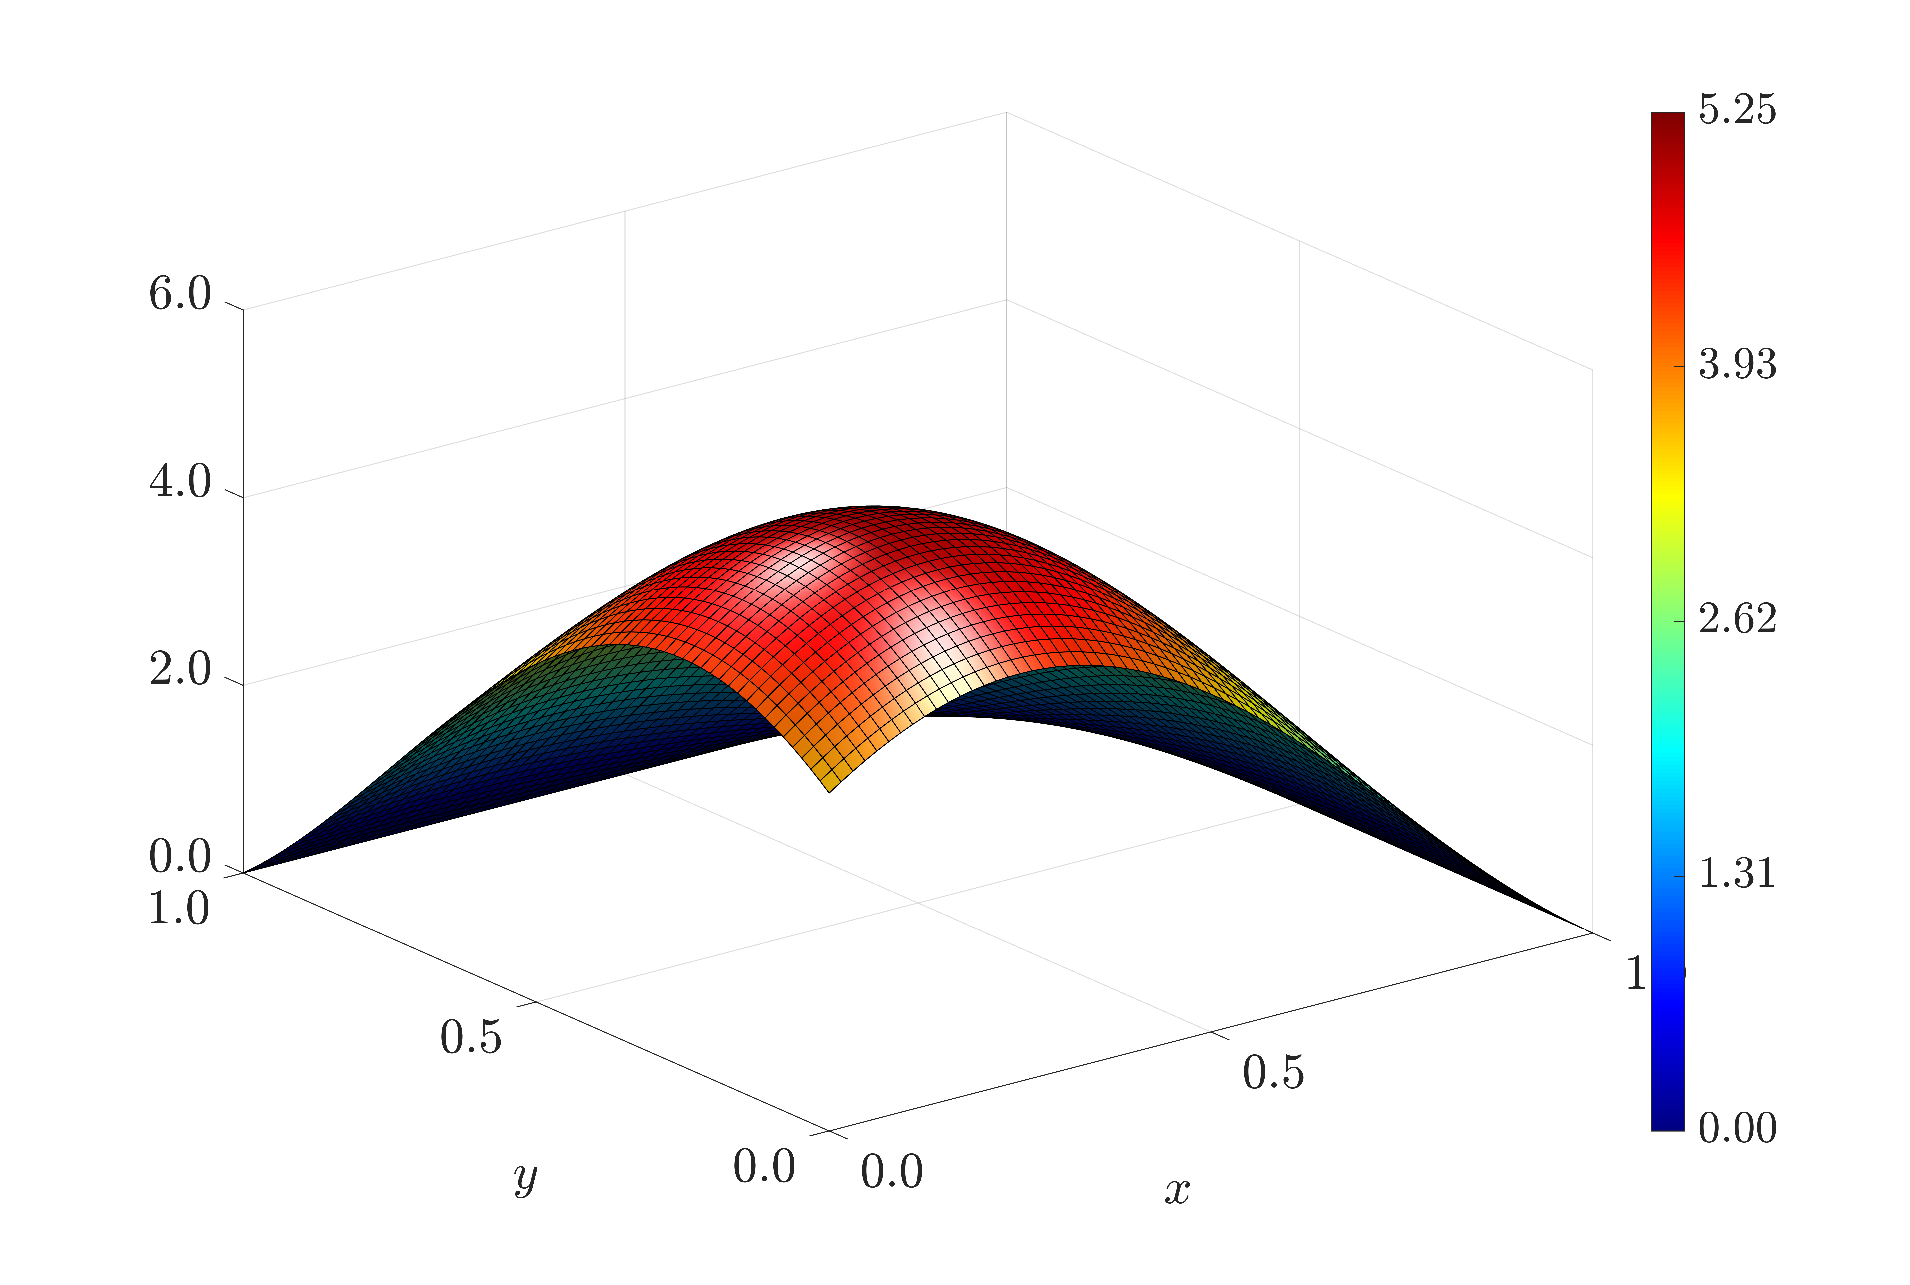
\includegraphics[width=\textwidth]{figures/Case12/UCM/Solutions/Exact_Surf_NormErr_2nd_Betann_0.1_Re_1_Wi_1_epsilon_0_xi_0_alphaG_0_Dt_1e-06_at_0.05_tipsim_1_MMS_12_Txx.eps}
            \caption{$\overline{T}_{xx}$}
            \label{fig_solexaTxxCase1}
        \end{subfigure}
        \vspace{0.2cm}
        \begin{subfigure}[b]{.47\textwidth}
            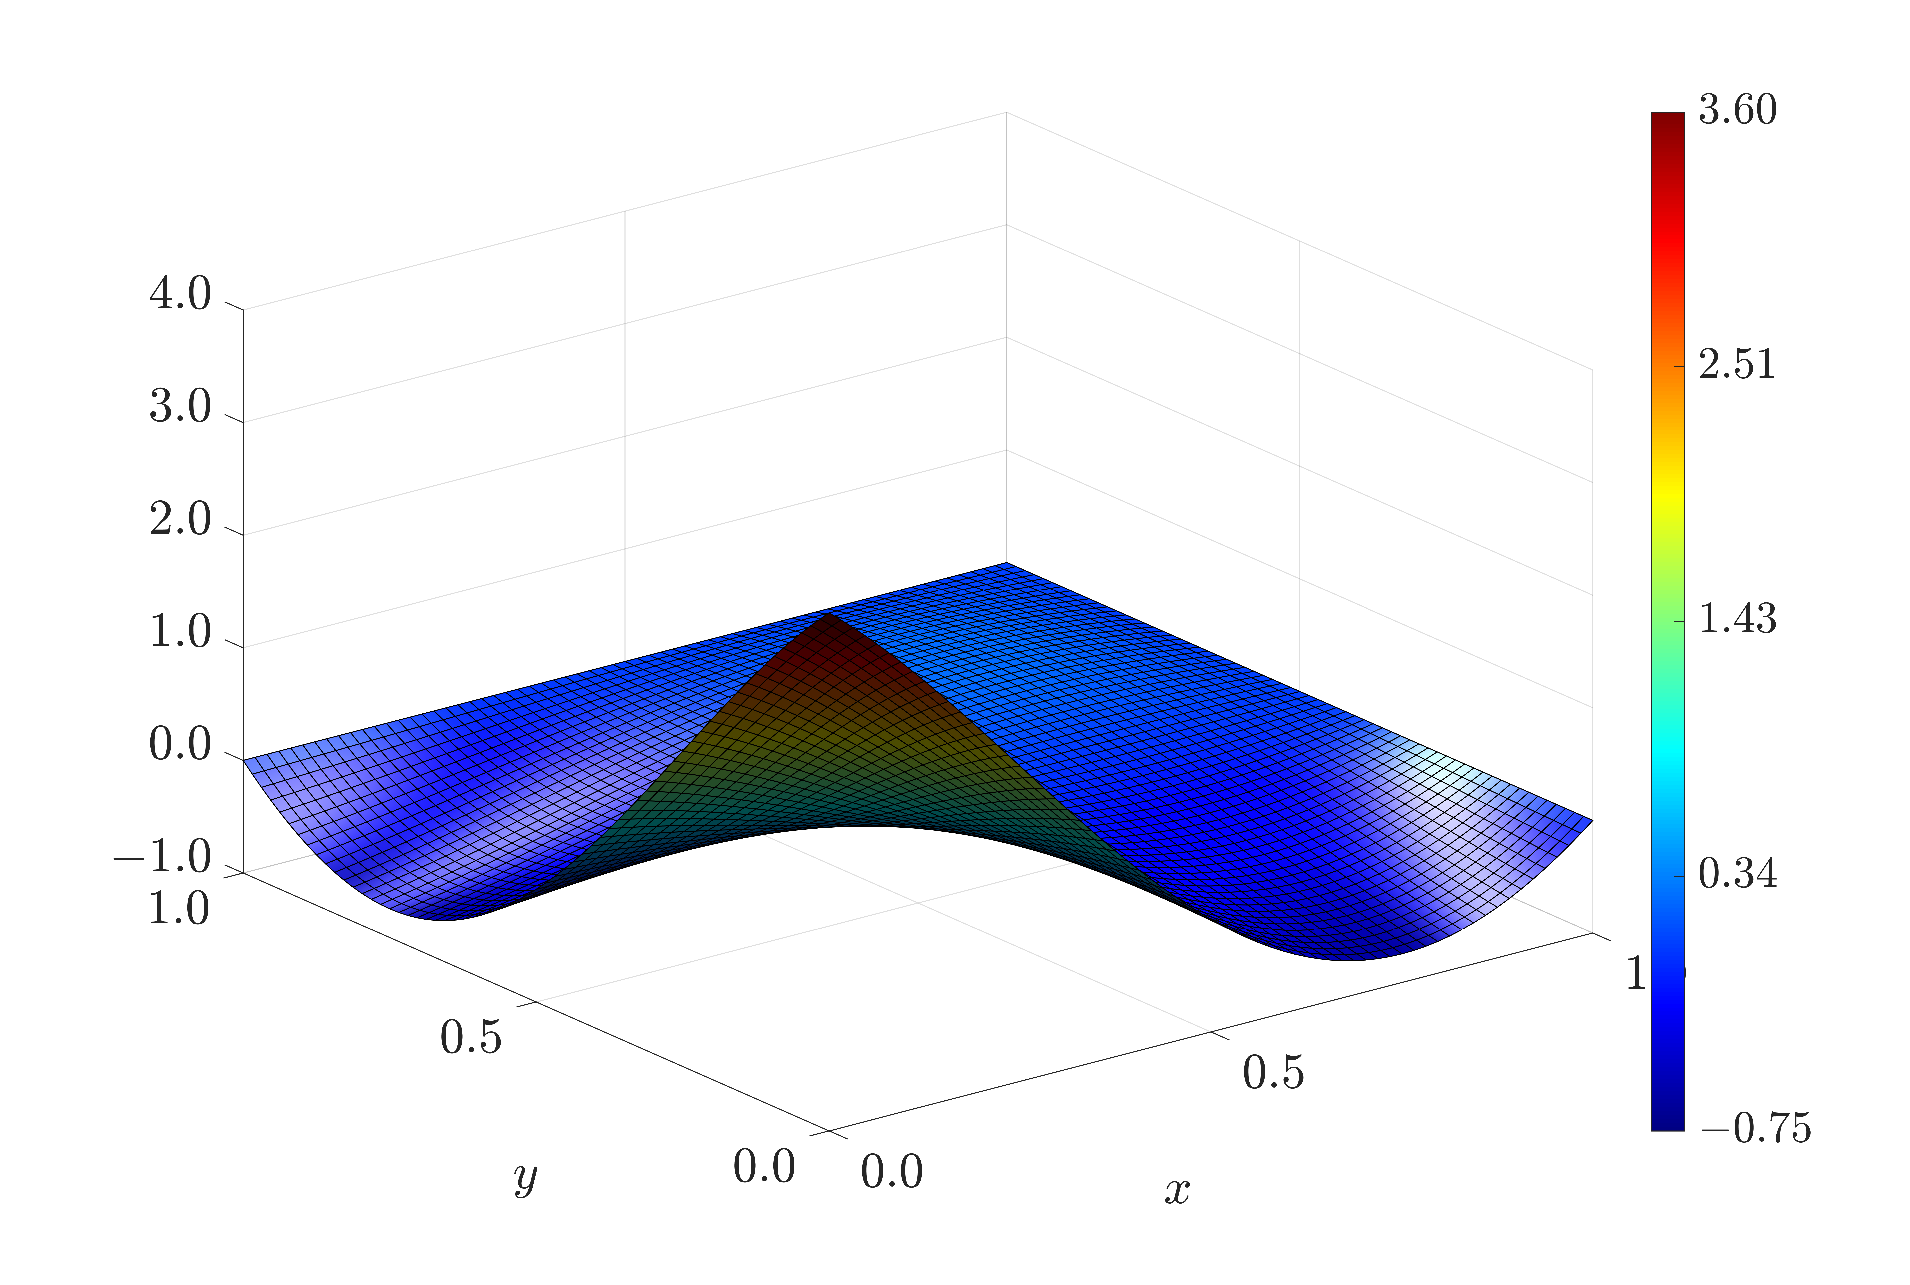
\includegraphics[width=\textwidth]{figures/Case12/UCM/Solutions/Exact_Surf_NormErr_2nd_Betann_0.1_Re_1_Wi_1_epsilon_0_xi_0_alphaG_0_Dt_1e-06_at_0.05_tipsim_1_MMS_12_Txy.eps}
            \caption{$\overline{T}_{xy}$}
            \label{fig_solexaTxyCase1}
        \end{subfigure}
        \begin{subfigure}[b]{.47\textwidth}
            \includegraphics[width=\textwidth]{figures/Case12/UCM/Solutions/Exact_Surf_NormErr_2nd_Betann_0.1_Re_1_Wi_1_epsilon_0_xi_0_alphaG_0_Dt_1e-06_at_0.05_tipsim_1_MMS_12_Tyy.eps}
            \caption{$\overline{T}_{yy}$}
            \label{fig_solexaTyyCase1}
        \end{subfigure}
	\fdadospesquisa
\end{figure}

As Figuras~\ref{fig_U_m_u_sol_num_case1streamline2} e \ref{fig_T_xxxyyy_sol_num_case1streamline2} apresentam as linhas de corrente das soluções manufaturadas no regime de estado estacionário, utilizando os parâmetros $\beta_{nn} = 0.1$ e $a = 0.05$. Além disso, essas figuras mostram as linhas de corrente juntamente com um mapa de contorno das soluções manufaturadas no mesmo regime, confirmando que o padrão de escoamento das soluções segue o comportamento típico do problema da cavidade com tampa deslizante, conforme apresentado em \citeonline{bruneau20062d}.
\begin{figure}[H]
        \centering
        \caption{Mapas de cores das soluções manufaturadas no regime de estado estacionário para o campo de velocidades $(\overline{u},\tilde{v})$, vorticidade $(\tilde{\omega_{z}})$ e função de corrente $(\tilde{\psi})$, considerando $a = 0.05$ em $t=0.1$}
        \label{fig_U_m_u_sol_num_case1streamline2}
        \begin{subfigure}[b]{.47\textwidth}
            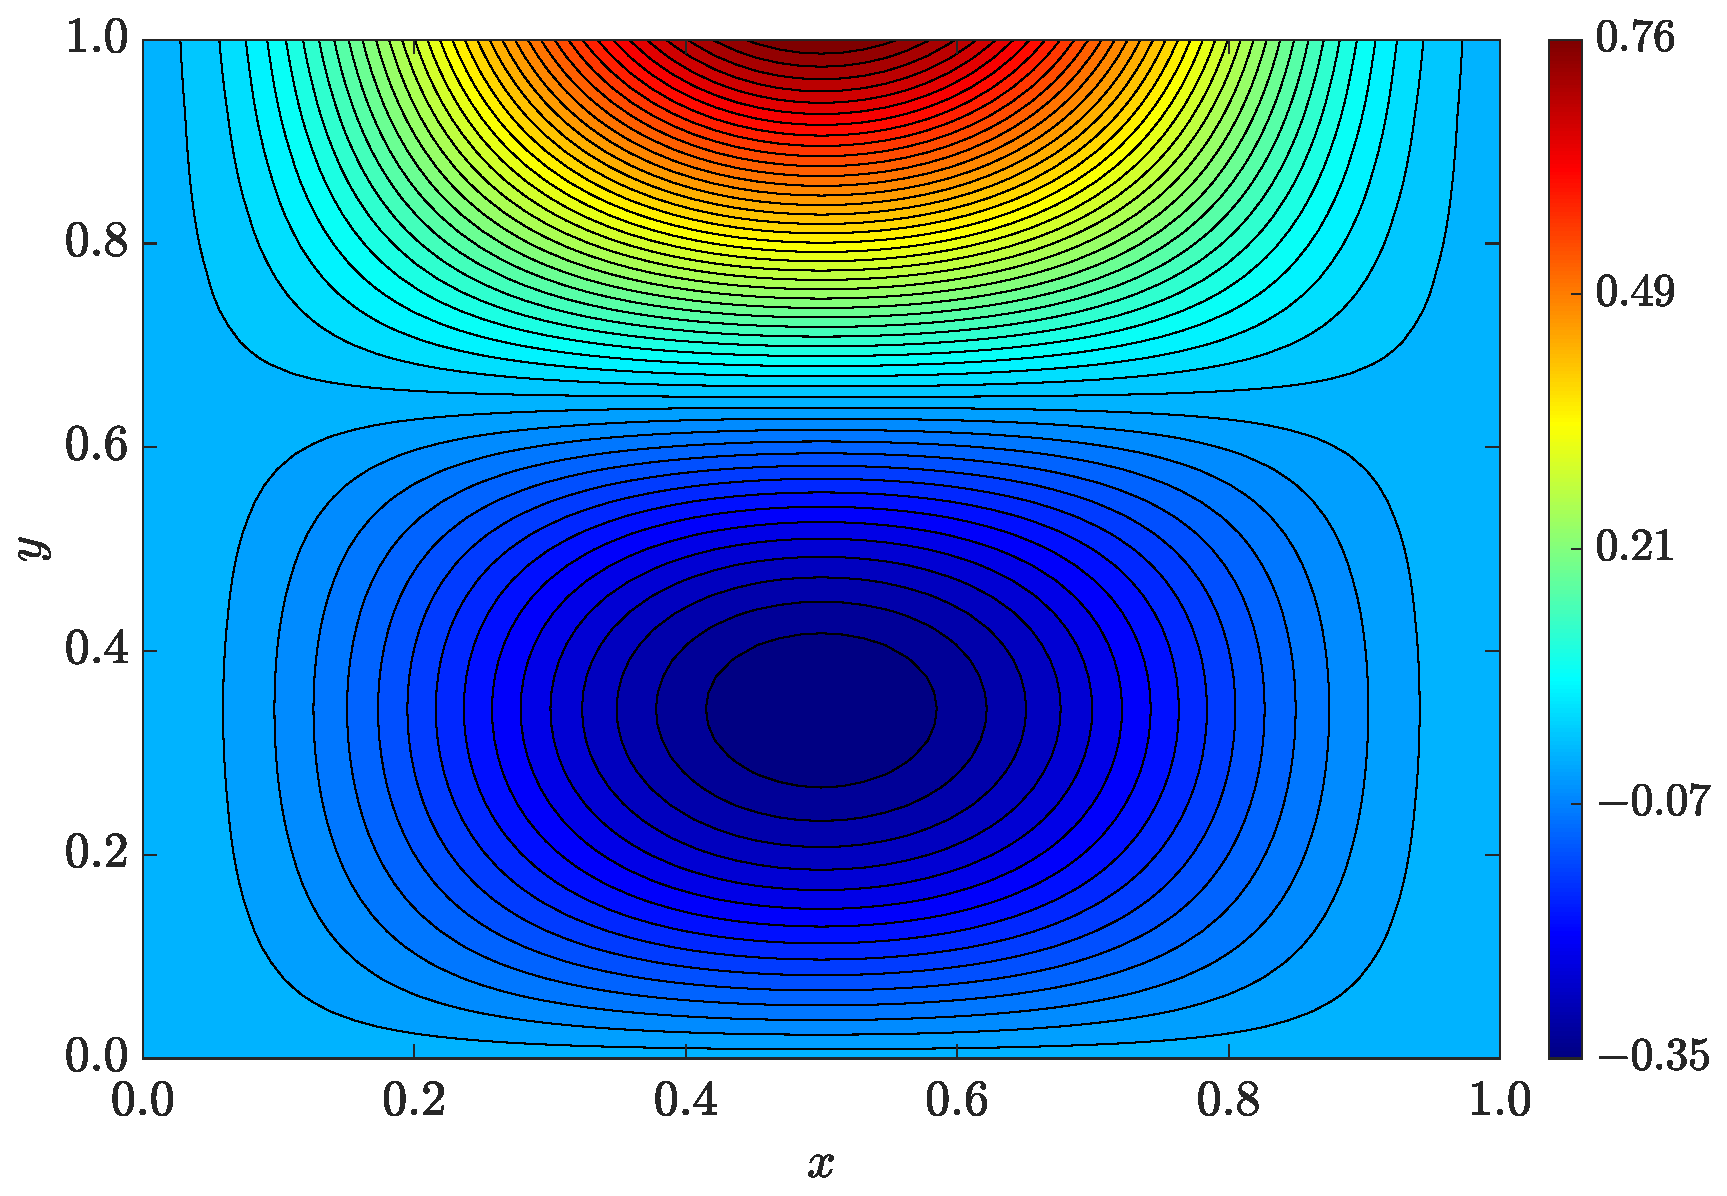
\includegraphics[width=\textwidth]{figures/Case12/UCM/Solutions/Exact_Map_NormErr_2nd_Betann_0.1_Re_1_Wi_1_epsilon_0_xi_0_alphaG_0_Dt_1e-06_at_0.05_tipsim_1_MMS_12_U.eps}
            \caption{$\overline{u}$}
            \label{fig_solexaustreamlineCase1}
        \end{subfigure}
        \vspace{0.2cm}
        \begin{subfigure}[b]{.47\textwidth}
            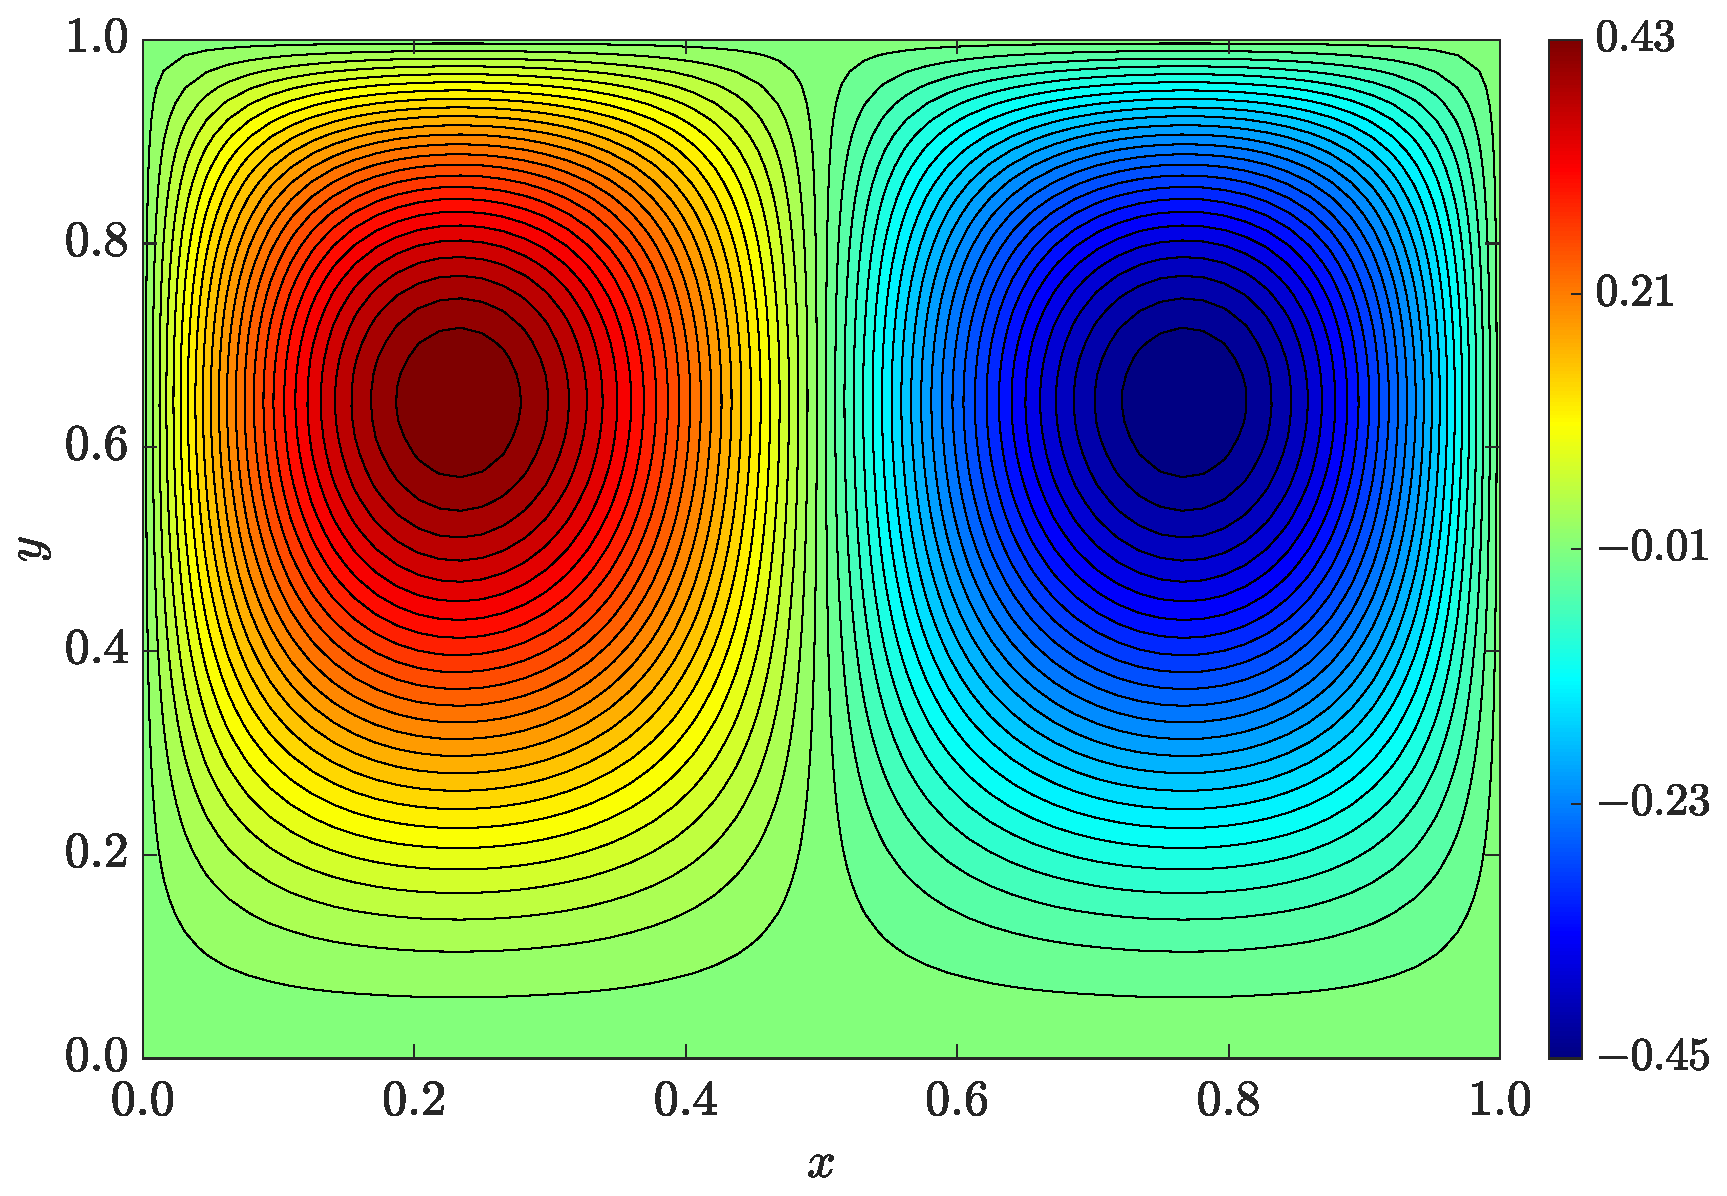
\includegraphics[width=\textwidth]{figures/Case12/UCM/Solutions/Exact_Map_NormErr_2nd_Betann_0.1_Re_1_Wi_1_epsilon_0_xi_0_alphaG_0_Dt_1e-06_at_0.05_tipsim_1_MMS_12_V.eps}
            \caption{$\widetilde{v}$}
            \label{fig_solexavstreamlineCase1}
        \end{subfigure}
        \begin{subfigure}[b]{.47\textwidth}
            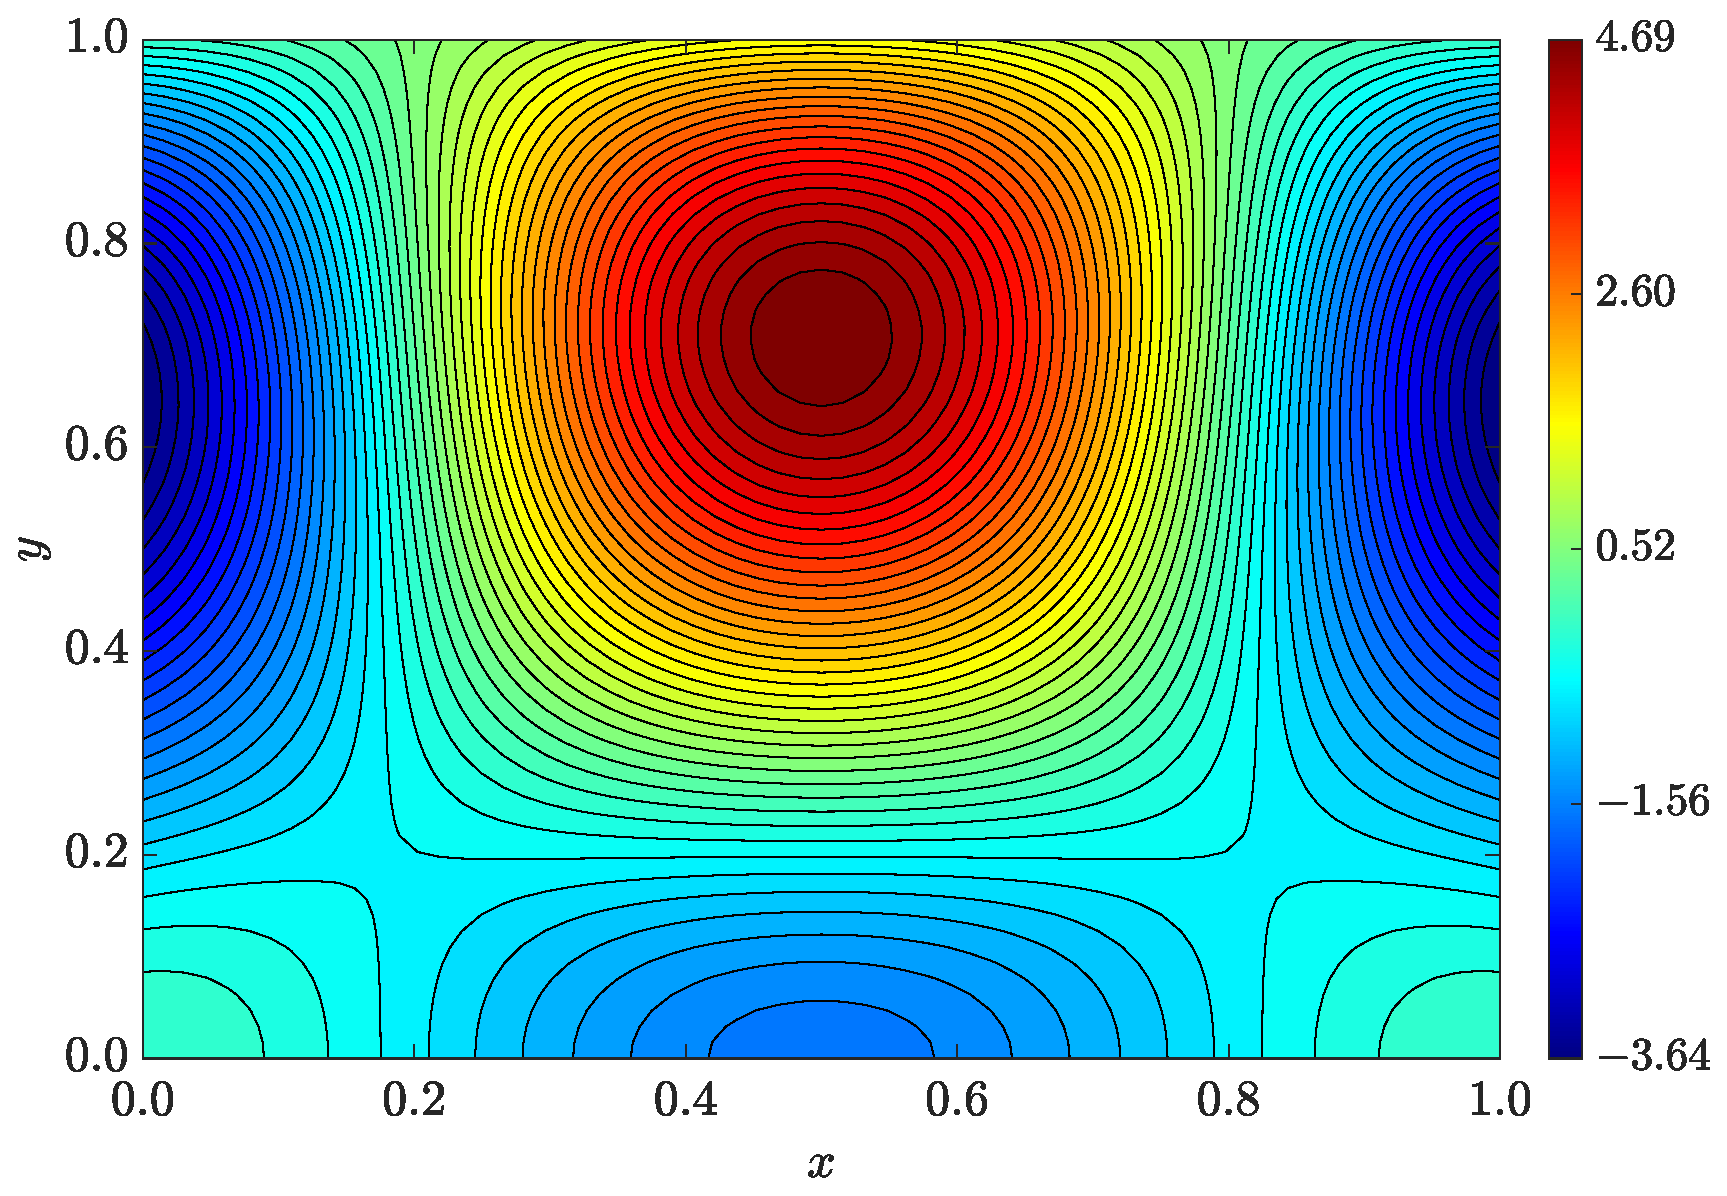
\includegraphics[width=\textwidth]{figures/Case12/UCM/Solutions/Exact_Map_NormErr_2nd_Betann_0.1_Re_1_Wi_1_epsilon_0_xi_0_alphaG_0_Dt_1e-06_at_0.05_tipsim_1_MMS_12_Wz.eps}
            \caption{$\widetilde{\omega_{z}}$}
            \label{fig_solexawzstreamlineCase1}
        \end{subfigure}
        \vspace{0.2cm}
        \begin{subfigure}[b]{.47\textwidth}
            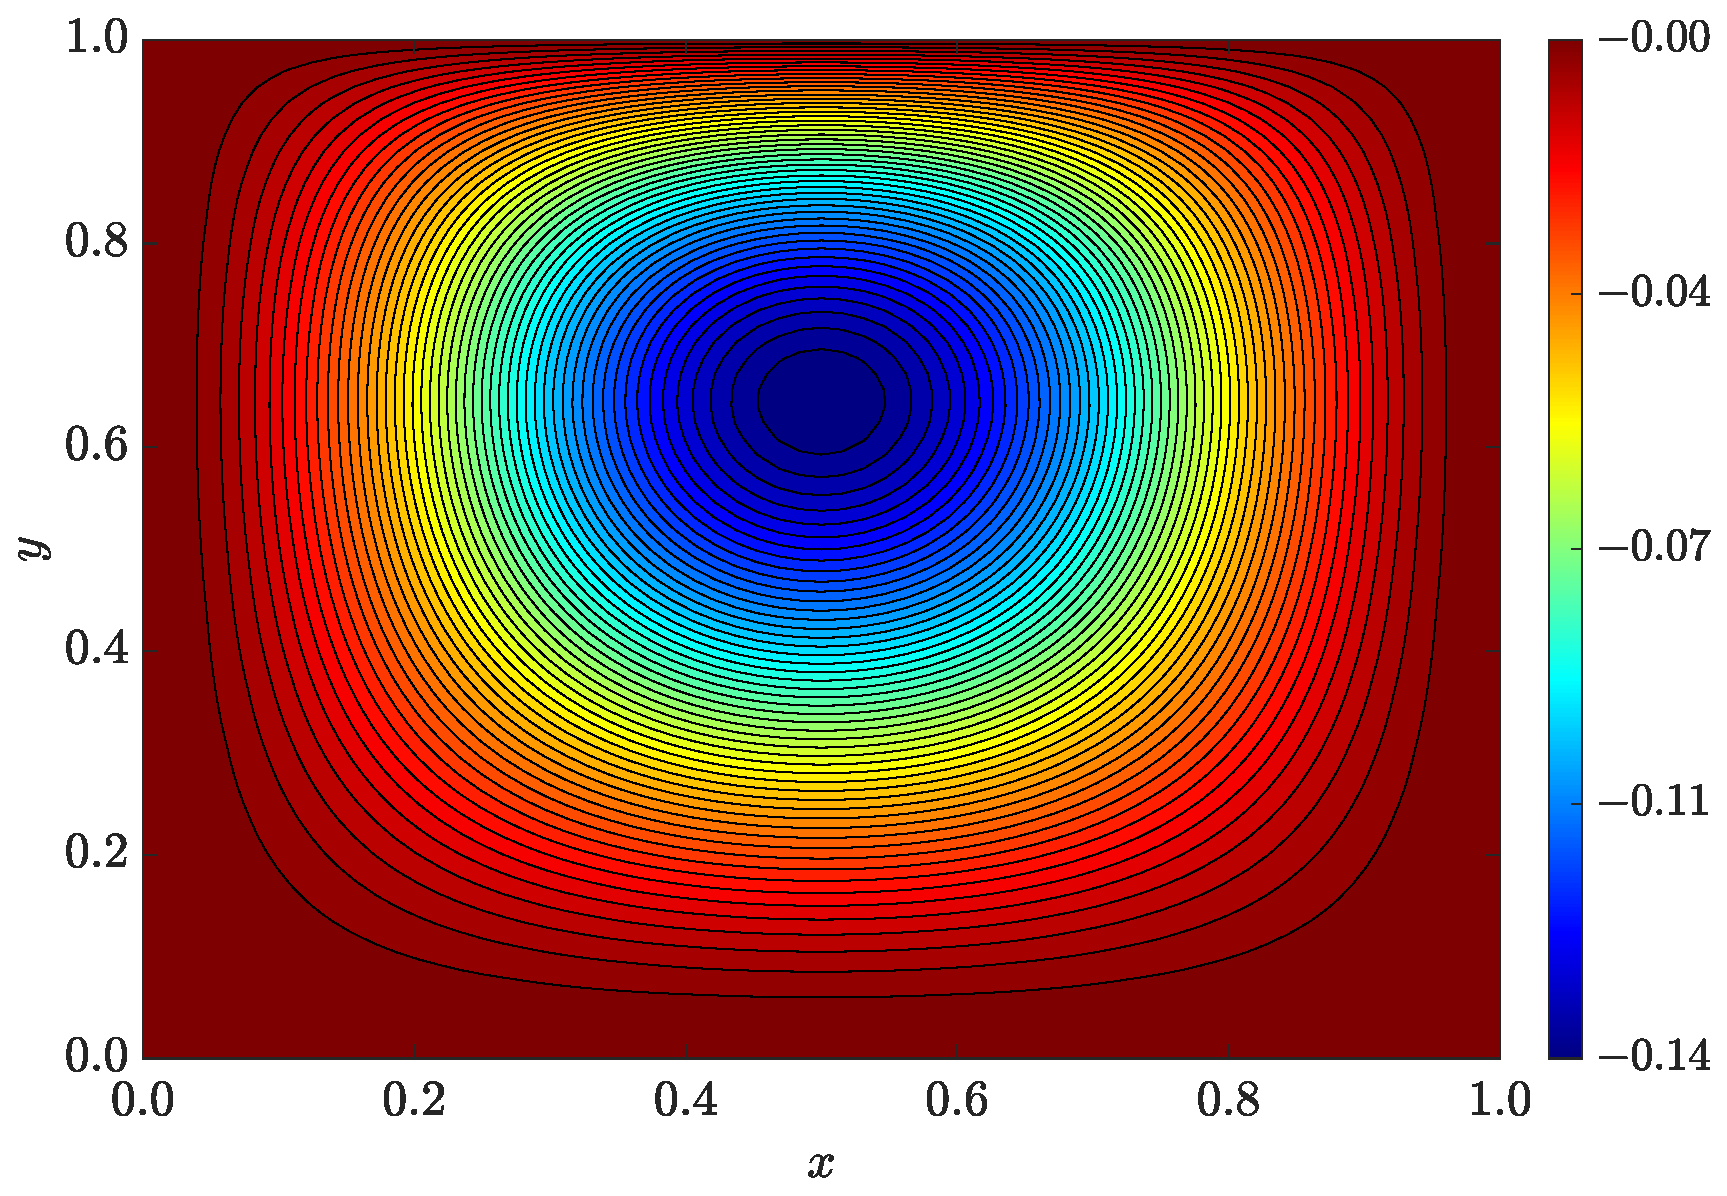
\includegraphics[width=\textwidth]{figures/Case12/UCM/Solutions/Exact_Map_NormErr_2nd_Betann_0.1_Re_1_Wi_1_epsilon_0_xi_0_alphaG_0_Dt_1e-06_at_0.05_tipsim_1_MMS_12_Psi.eps}
            \caption{$\widetilde{\psi}$}
            \label{fig_solexapsistreamlineCase1}
        \end{subfigure}
        \fdadospesquisa
\end{figure}

\begin{figure}[H]
        \centering
	\caption{Mapas de cores das soluções manufaturadas no regime de estado estacionário para os tensores, considerando $a = 0.05$ em $t = 0.1$}
        \label{fig_T_xxxyyy_sol_num_case1streamline2}
	\begin{subfigure}[b]{.47\textwidth}
            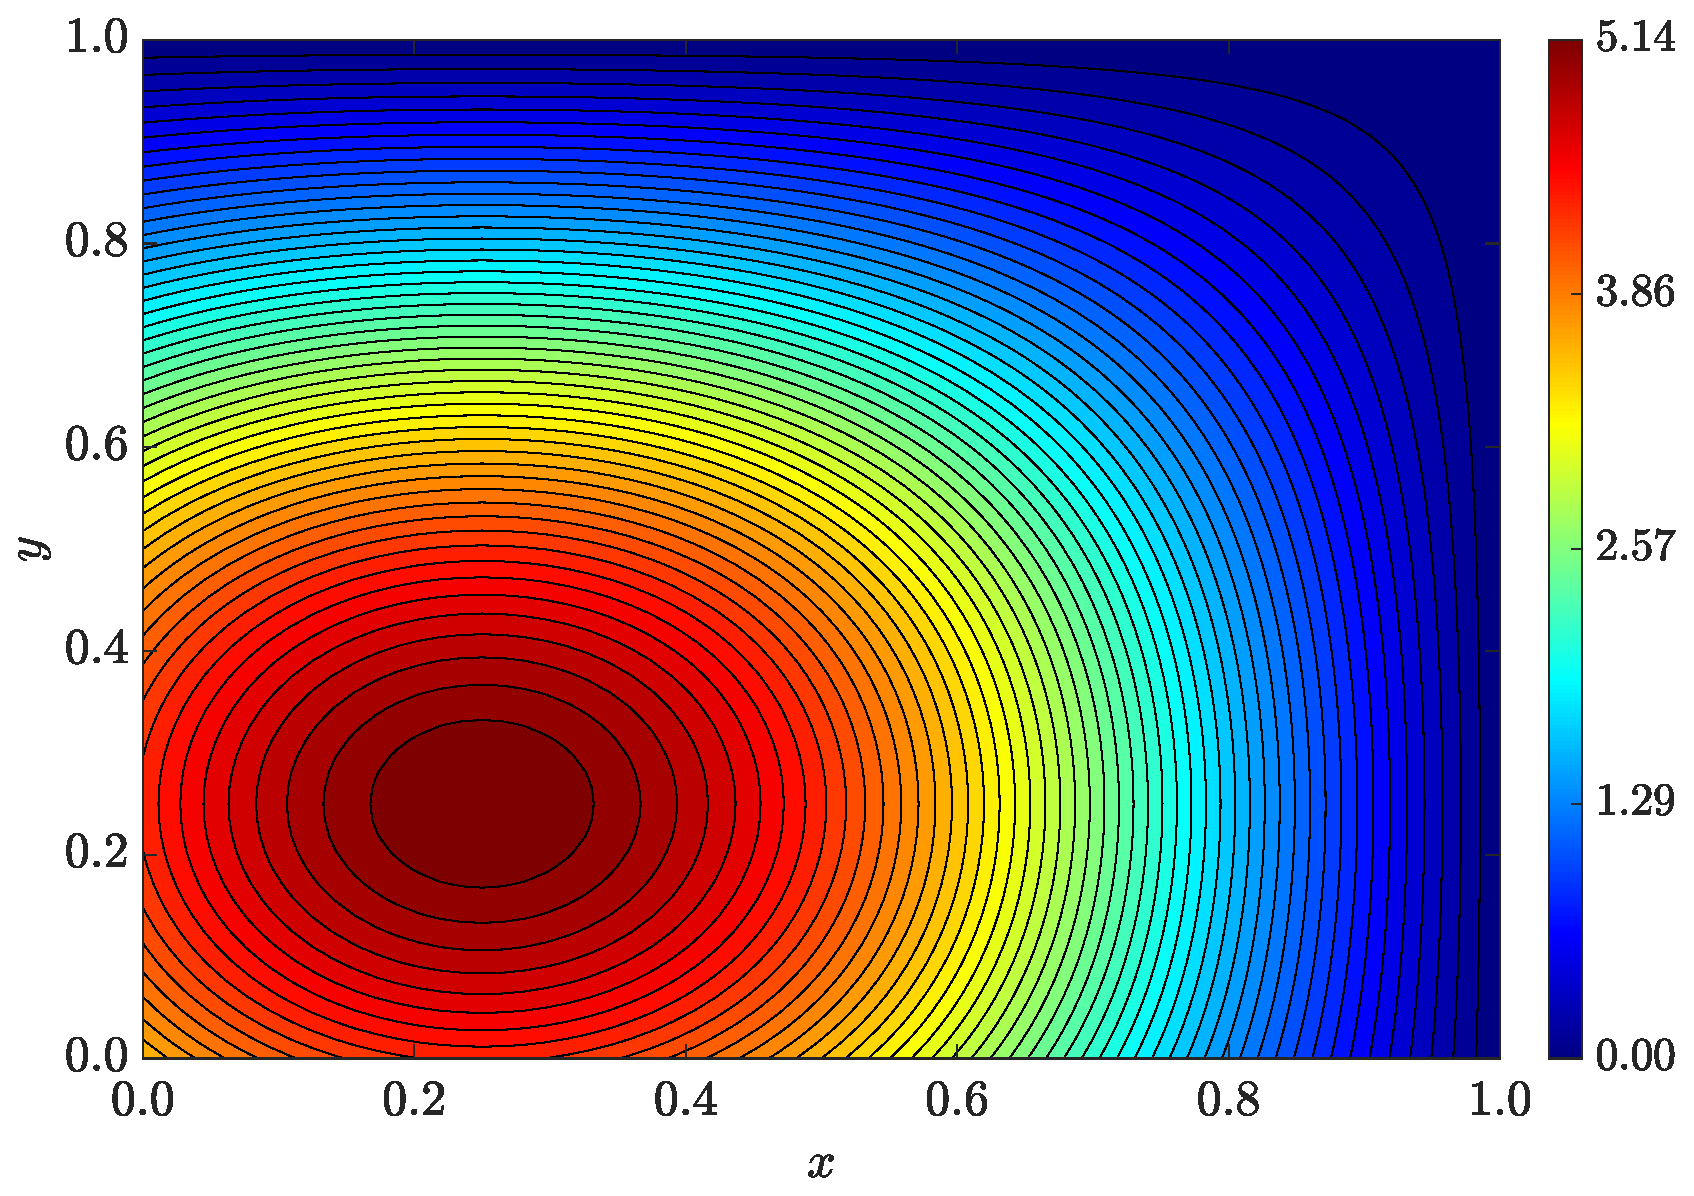
\includegraphics[width=\textwidth]{figures/Case12/UCM/Solutions/Exact_Map_NormErr_2nd_Betann_0.1_Re_1_Wi_1_epsilon_0_xi_0_alphaG_0_Dt_1e-06_at_0.05_tipsim_1_MMS_12_Txx.eps}
            \caption{$\overline{T}_{xx}$}
            \label{fig_solexatxxstreamlineCase1}
        \end{subfigure}
        \begin{subfigure}[b]{.47\textwidth}
            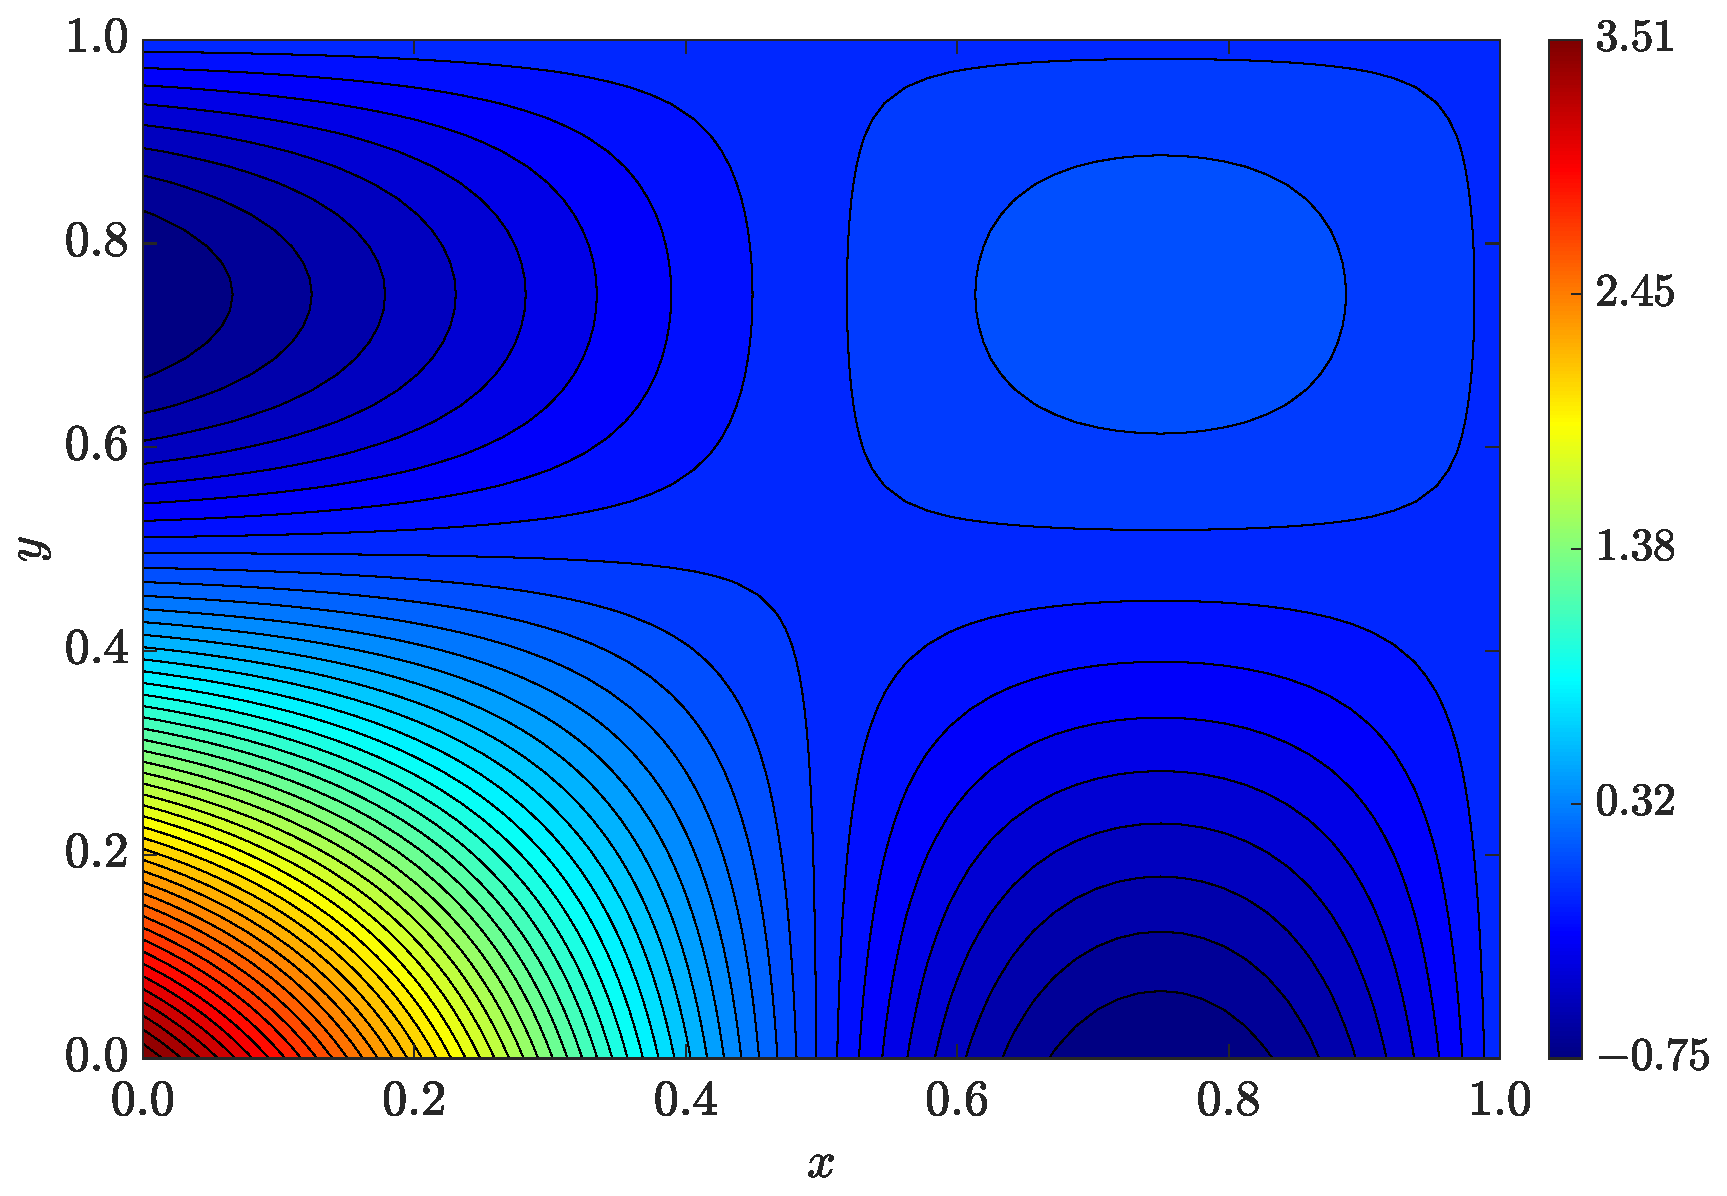
\includegraphics[width=\textwidth]{figures/Case12/UCM/Solutions/Exact_Map_NormErr_2nd_Betann_0.1_Re_1_Wi_1_epsilon_0_xi_0_alphaG_0_Dt_1e-06_at_0.05_tipsim_1_MMS_12_Txy.eps}
            \caption{$\overline{T}_{xy}$}
            \label{fig_solexatxystreamlineCase1}
        \end{subfigure}
        \vspace{0.2cm}
        \begin{subfigure}[b]{.47\textwidth}
            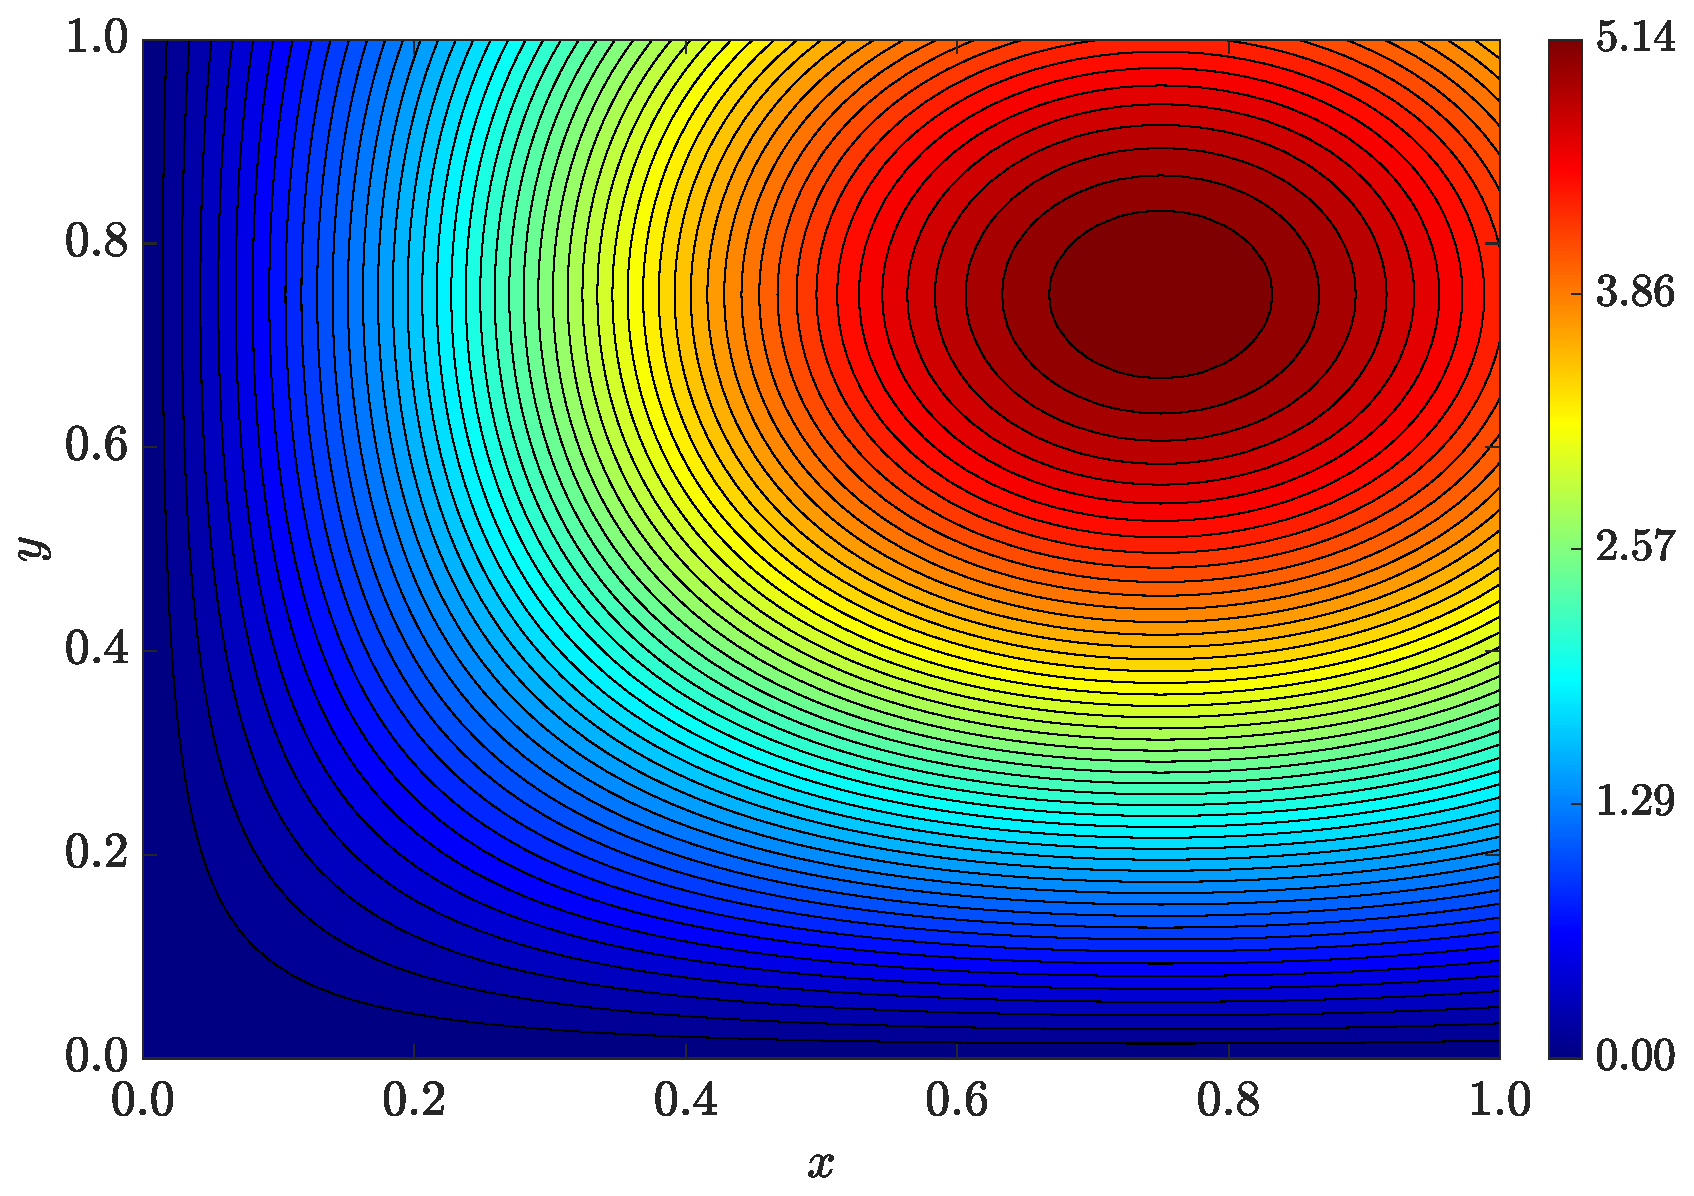
\includegraphics[width=\textwidth]{figures/Case12/UCM/Solutions/Exact_Map_NormErr_2nd_Betann_0.1_Re_1_Wi_1_epsilon_0_xi_0_alphaG_0_Dt_1e-06_at_0.05_tipsim_1_MMS_12_Tyy.eps}
            \caption{$\overline{T}_{yy}$}
            \label{fig_solexatyystreamlineCase1}
        \end{subfigure}
        \fdadospesquisa
\end{figure}

A partir deste ponto, será adotada uma convenção de notação para distinguir as soluções numéricas obtidas pelo código das soluções manufaturadas utilizadas como referência analítica. Todas as variáveis representadas por letras maiúsculas (por exemplo, $U$, $V$, $\Omega_z$, $\Psi$, $T_{xx}$, $T_{xy}$ e $T_{yy}$) correspondem às soluções numéricas computadas nas simulações. Por outro lado, as variáveis acompanhadas de til ($\widetilde{\cdot}$) ou barra superior ($\overline{\cdot}$) representam as soluções manufaturadas, derivadas simbolicamente e utilizadas para a verificação dos resultados. Essa distinção é utilizada para a interpretação dos gráficos, tabelas e análises de erro apresentadas nas próximas seções.

\subsection{Caso de verificação usando o modelo UCM}

As simulações numéricas realizadas para verificar o código de alta ordem desenvolvido para escoamentos de fluidos viscoelásticos foram configuradas utilizando o modelo UCM, com números de Reynolds variando entre $Re = 1,\ 10,\ 100,\ 400$ e $1000$, número de Weissenberg $Wi = 1,\ 5$ e $10$. Para este modelo, a razão de viscosidade do solvente foi fixada em $\beta_{nn} = 0$, representando o comportamento puramente viscoelástico sem influência da viscosidade do solvente, com o objetivo de avaliar o desempenho do modelo em diferentes regimes de escoamento viscoelástico.

Dado que os resultados obtidos para as diferentes combinações de parâmetros apresentaram comportamentos qualitativamente semelhantes, assim apresenta-se detalhadamente apenas um dos casos simulados. Essa escolha visa evitar repetições e tornar a análise mais objetiva, sem prejuízo à generalidade das conclusões sobre a acurácia e estabilidade do método numérico proposto. A \autoref{UCMerror1} apresenta os gráficos de erro para os componentes do campo de velocidade, vorticidade e função de corrente, enquanto a \autoref{UCMerror2} complementa essa análise mostrando os erros associados aos tensores no escoamento de fluido viscoelástico UCM. Esses gráficos mostram a evolução dos erros para $Re = 100$, $Wi = 1$ e $\beta_{nn} = 0$. Observou-se que, à medida que a malha é refinada, os erros diminuem consideravelmente, confirmando a eficácia do esquema numérico na captura das propriedades do escoamento.
\begin{figure}[H]
        \centering
	\caption{Erro para o campo de velocidades $(\overline{u},\tilde{v})$, vorticidade $(\tilde{\omega_{z}})$ e função de corrente $(\tilde{\psi})$, utilizando $Re=100$, $\beta_{nn} = 0$ e $Wi=1$ para o escoamento de fluido viscoelástico como o modelo UCM}
        \label{UCMerror1}
	\begin{subfigure}[b]{.47\textwidth}
            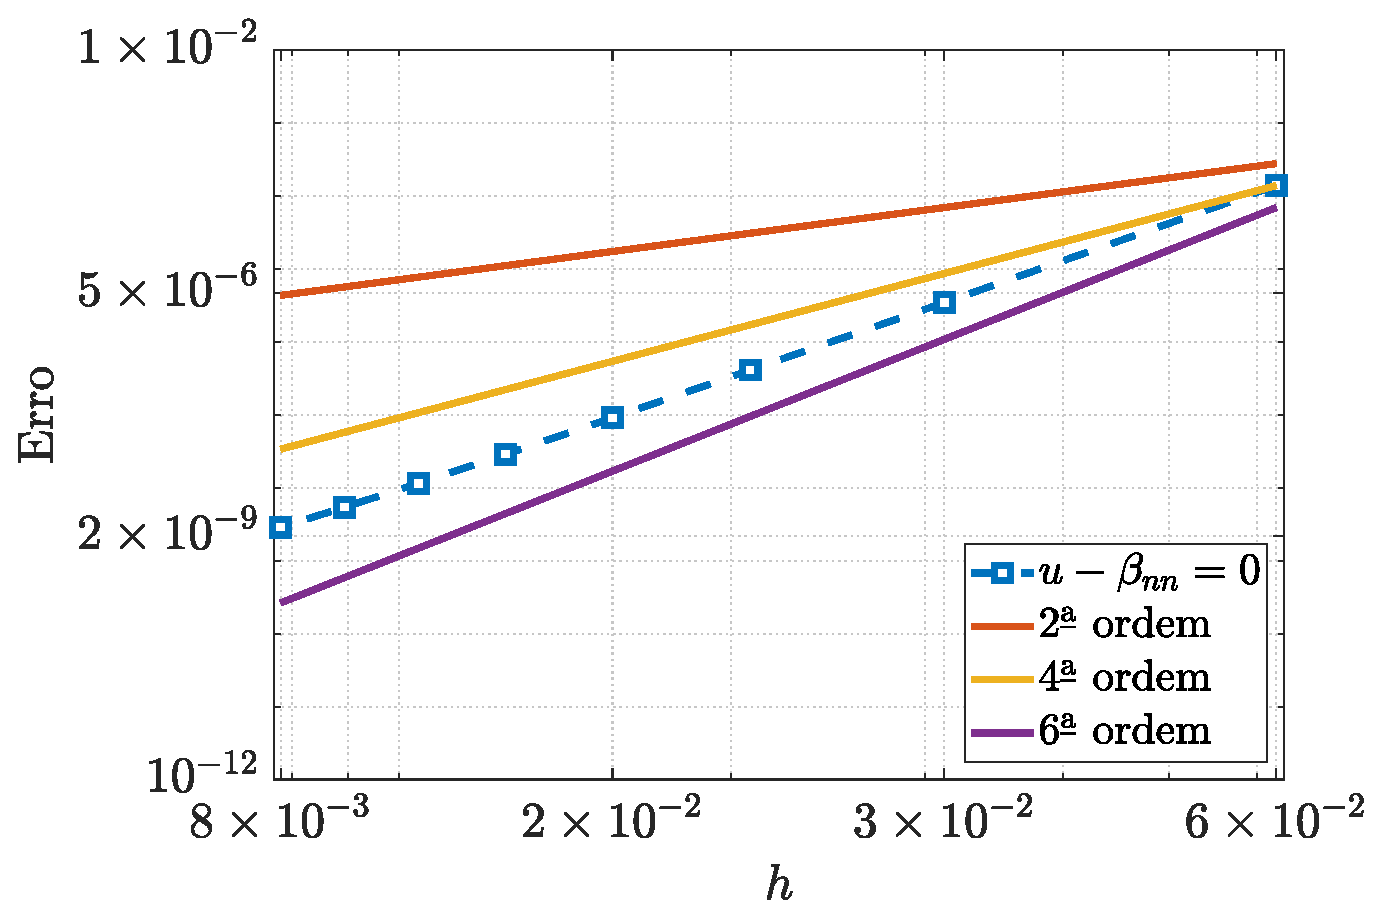
\includegraphics[width=\textwidth]{figures/Case12/UCM/Errors/NormErr_2nd_Re_100_Wi_1_epsilon_0_xi_0_alphaG_0_Dt_1e-06_at_0.05_tipsim_1_MMS_12_U.eps}
            \caption{$||U - \overline{u}||_{2}$}
            \label{error_u_2nd_Case1_ucm}
        \end{subfigure}
        \vspace{0.2cm}
        \qquad
        \begin{subfigure}[b]{.47\textwidth}
            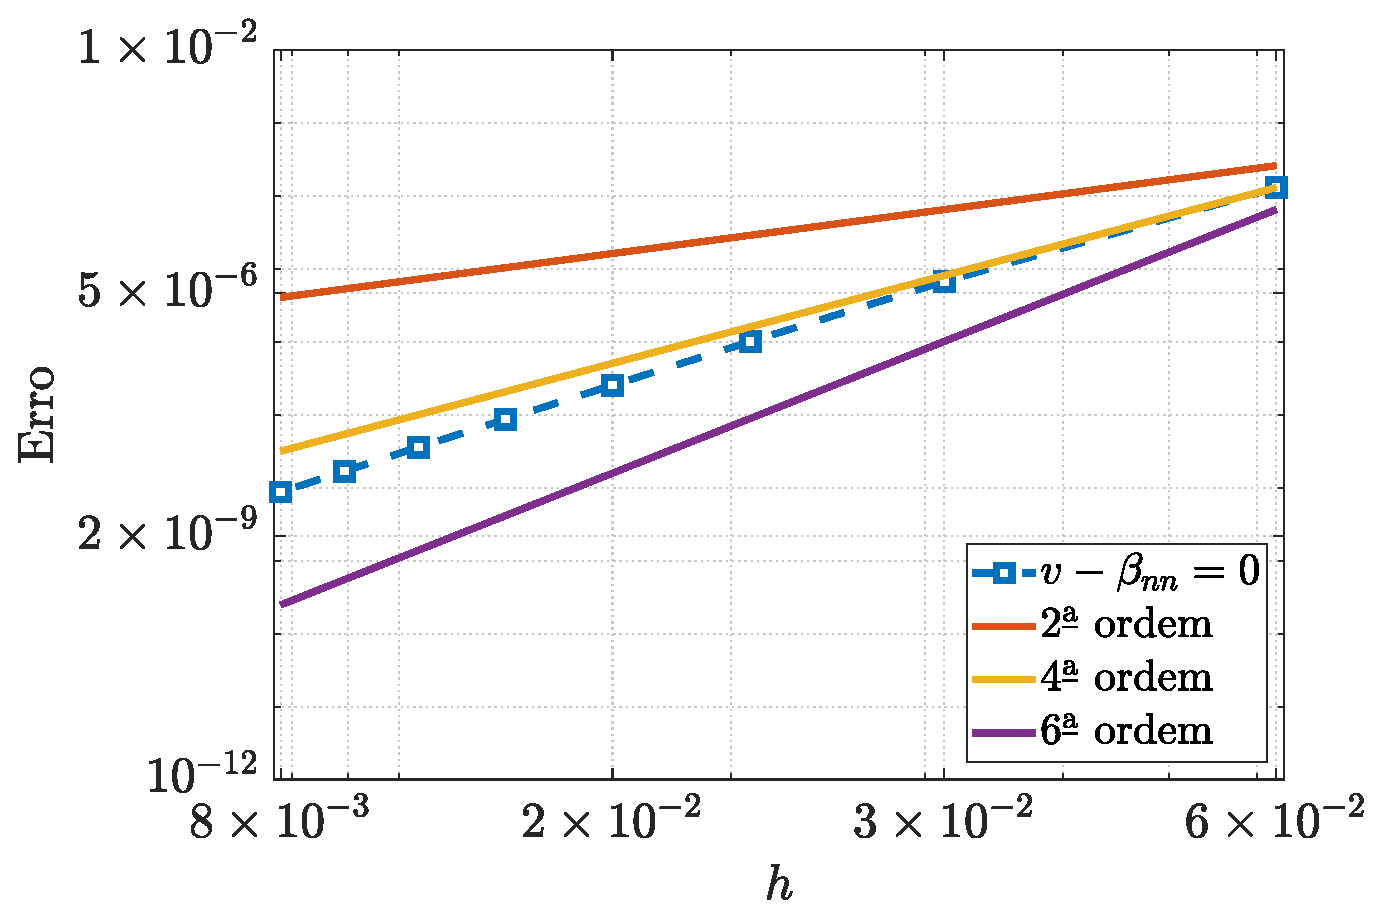
\includegraphics[width=\textwidth]{figures/Case12/UCM/Errors/NormErr_2nd_Re_100_Wi_1_epsilon_0_xi_0_alphaG_0_Dt_1e-06_at_0.05_tipsim_1_MMS_12_V.eps}
            \caption{$||V - \widetilde{v}||_{2}$}
            \label{error_v_2nd_Case1_ucm}
        \end{subfigure}
        \qquad
        \begin{subfigure}[b]{.47\textwidth}
            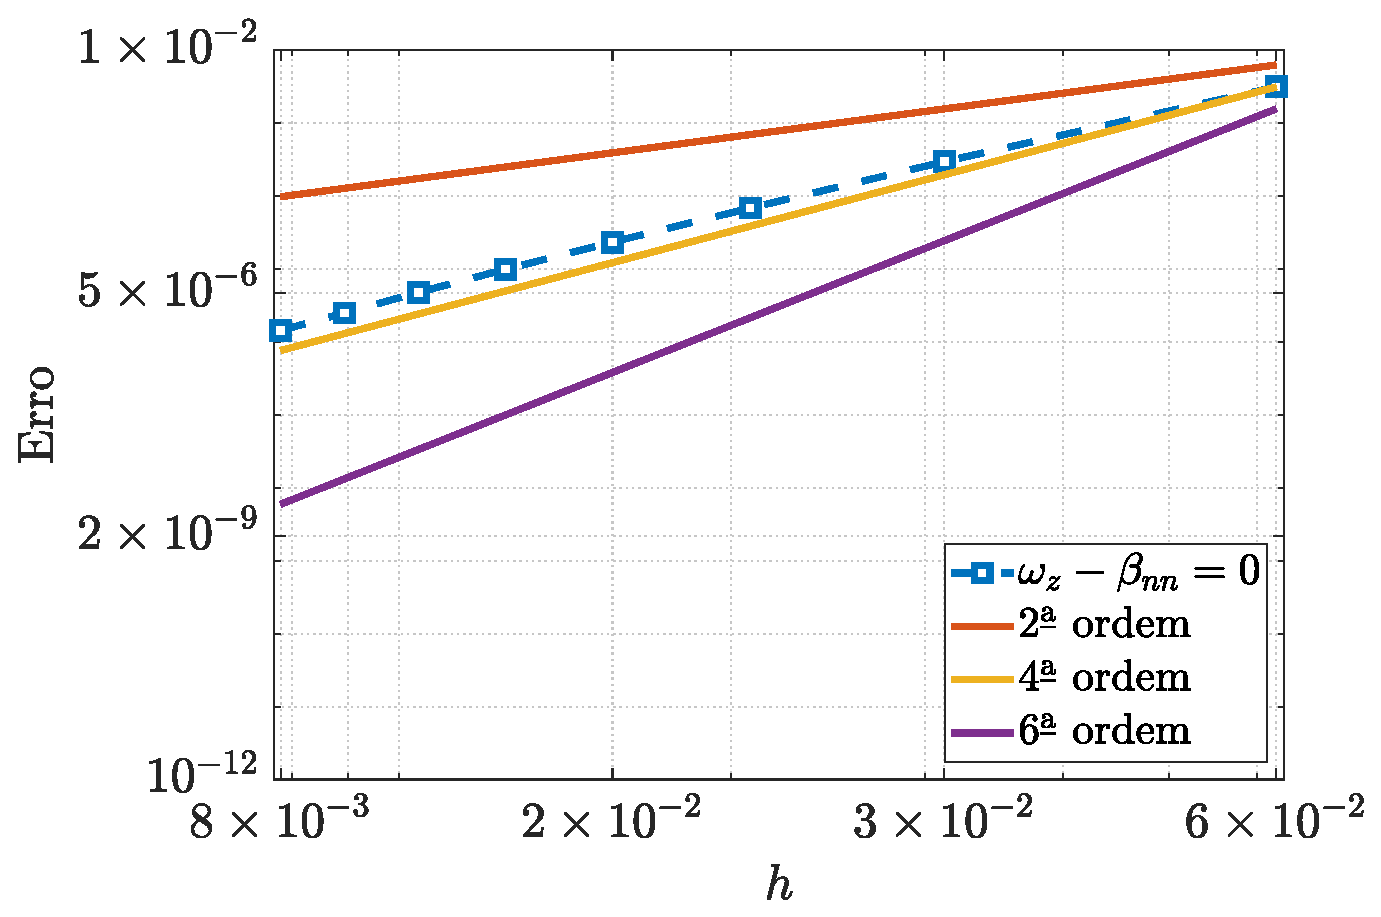
\includegraphics[width=\textwidth]{figures/Case12/UCM/Errors/NormErr_2nd_Re_100_Wi_1_epsilon_0_xi_0_alphaG_0_Dt_1e-06_at_0.05_tipsim_1_MMS_12_Wz.eps}
            \caption{$||\Omega_{z} - \widetilde{\omega_{z}}||_{2}$}
            \label{error_wz_2nd_Case1_ucm}
        \end{subfigure}
        \vspace{0.02cm}
        \qquad
        \begin{subfigure}[b]{.47\textwidth}
            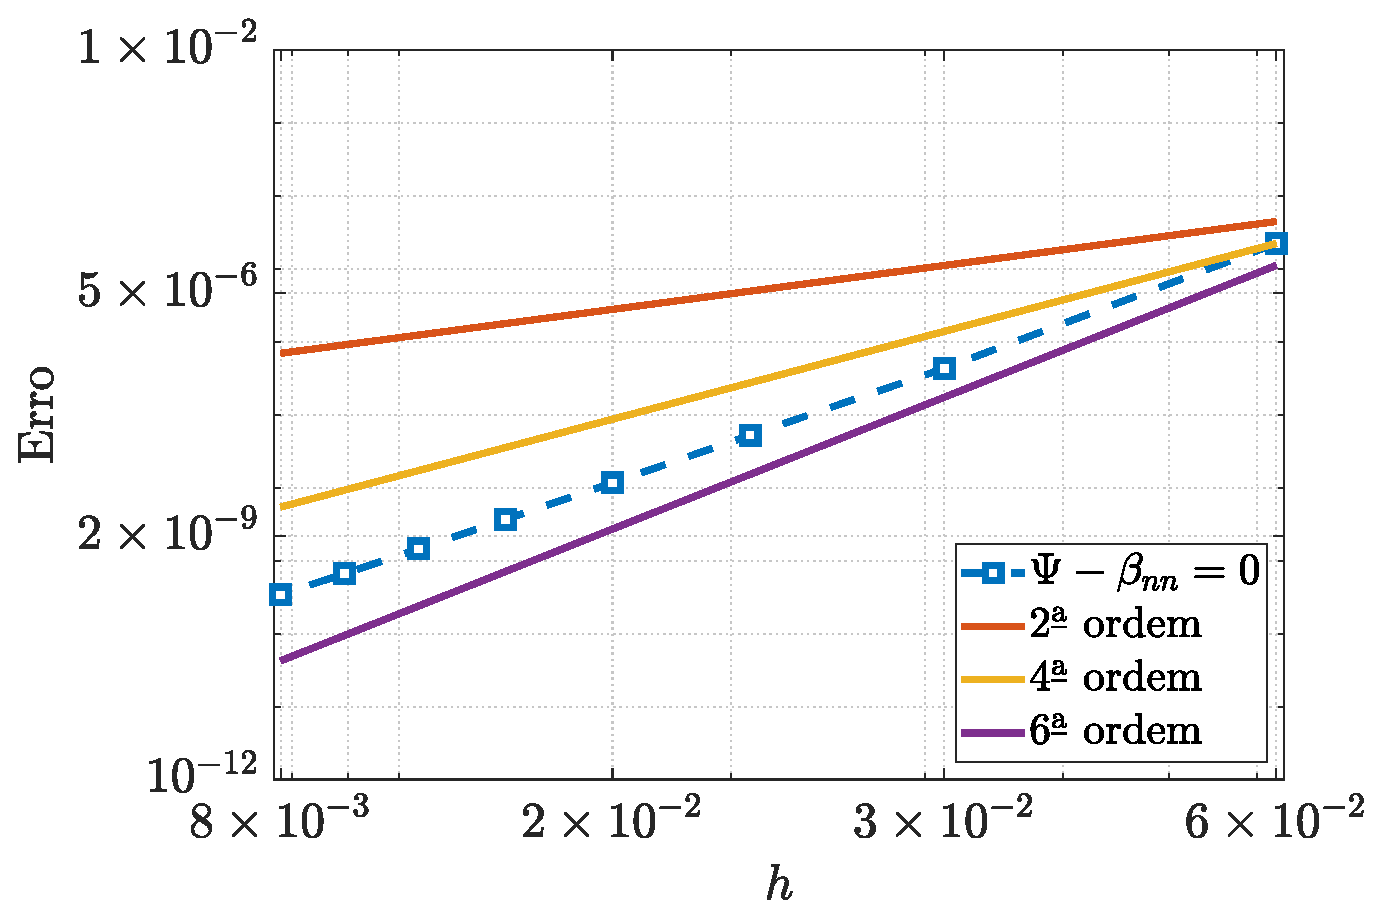
\includegraphics[width=\textwidth]{figures/Case12/UCM/Errors/NormErr_2nd_Re_100_Wi_1_epsilon_0_xi_0_alphaG_0_Dt_1e-06_at_0.05_tipsim_1_MMS_12_Psi.eps}
            \caption{$||\Psi - \widetilde{\Psi}||_{2}$}
            \label{error_psi_2nd_Case1_ucm}
        \end{subfigure}
        \fdadospesquisa
\end{figure}

\begin{figure}[H]
    \centering
    \caption{Erro para as componentes dos tensores de tensões, utilizando $Re=100$, $\beta_{nn} = 0$ e $Wi=1$ para o escoamento de fluido viscoelástico como o modelo UCM}
    \label{UCMerror2}
    \begin{subfigure}[b]{.47\textwidth}
        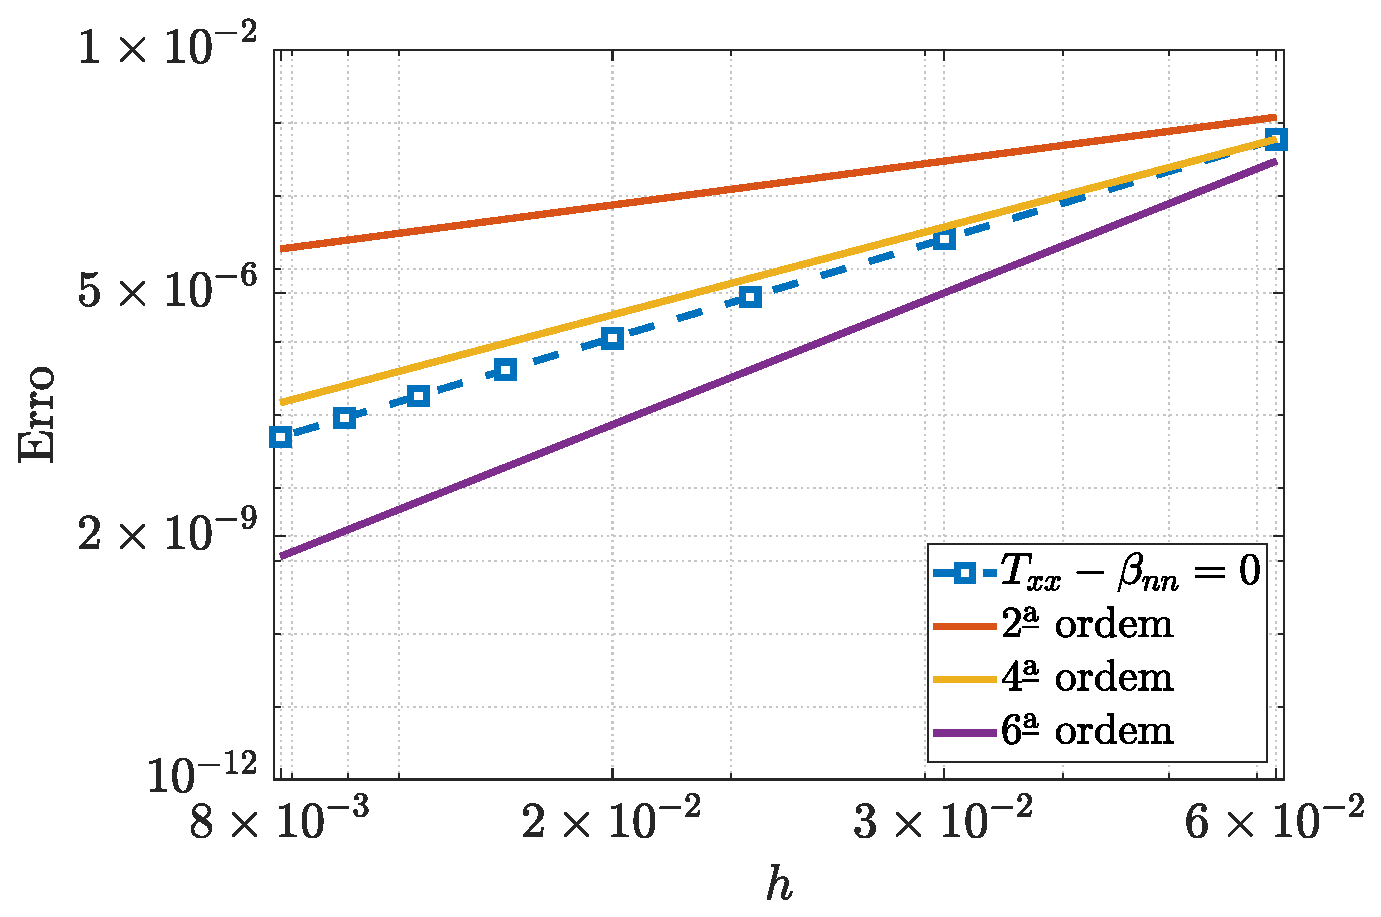
\includegraphics[width=\textwidth]{figures/Case12/UCM/Errors/NormErr_2nd_Re_100_Wi_1_epsilon_0_xi_0_alphaG_0_Dt_1e-06_at_0.05_tipsim_1_MMS_12_Txx.eps}
        \caption{$||T_{xx} - \overline{T}_{xx}||_{2}$}
        \label{error_txx_2nd_Case1_ucm}
    \end{subfigure}
    \vspace{0.2cm}
    \qquad
    \begin{subfigure}[b]{.47\textwidth}
        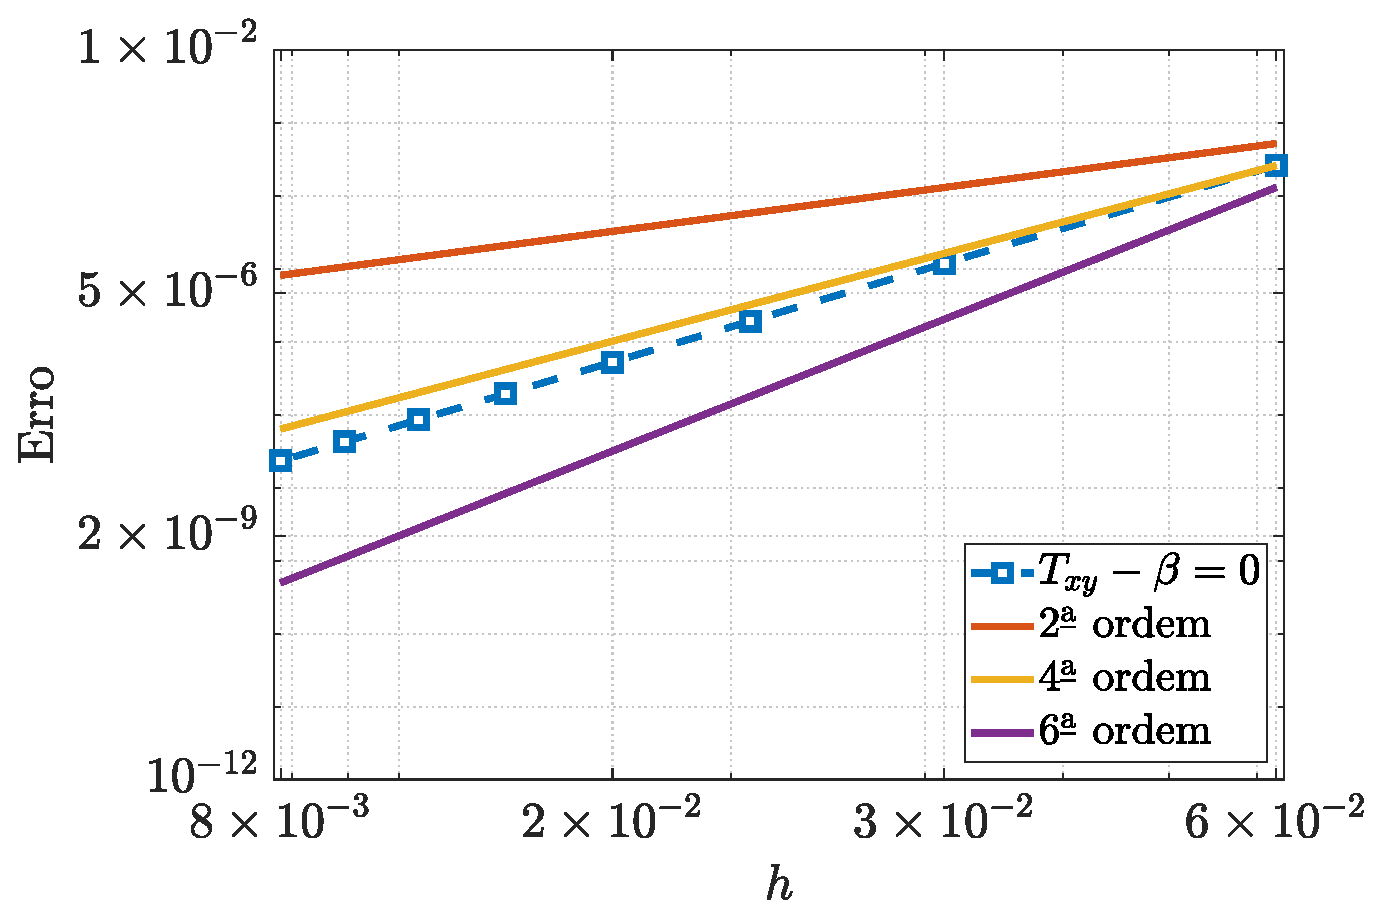
\includegraphics[width=\textwidth]{figures/Case12/UCM/Errors/NormErr_2nd_Re_100_Wi_1_epsilon_0_xi_0_alphaG_0_Dt_1e-06_at_0.05_tipsim_1_MMS_12_Txy.eps}
        \caption{$||T_{xy} - \overline{T}_{xy}||_{2}$}
        \label{error_txy_2nd_Case1_ucm}
    \end{subfigure}
    \qquad
    \begin{subfigure}[b]{.47\textwidth}
        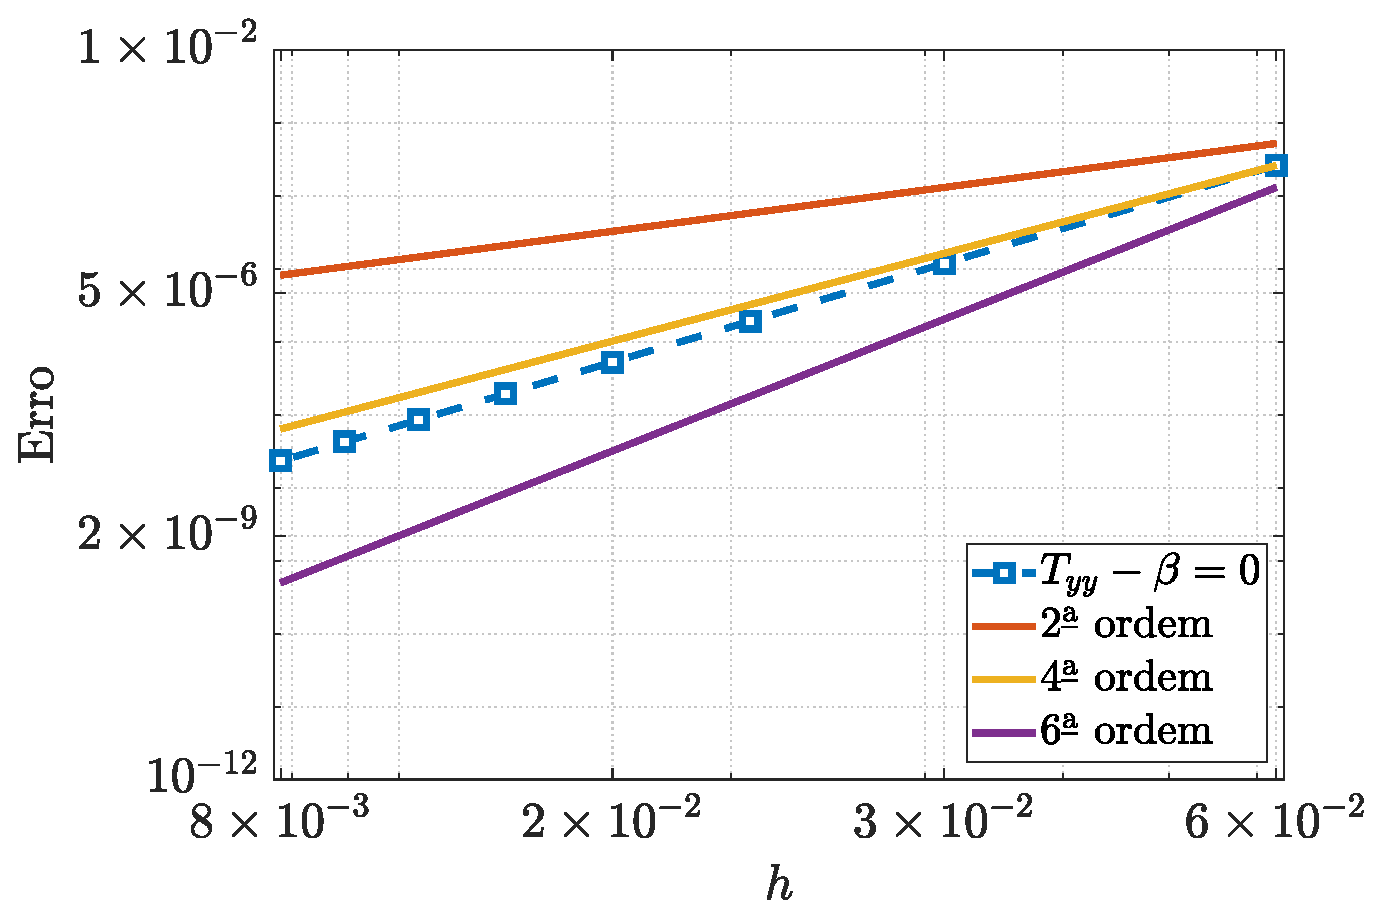
\includegraphics[width=\textwidth]{figures/Case12/UCM/Errors/NormErr_2nd_Re_100_Wi_1_epsilon_0_xi_0_alphaG_0_Dt_1e-06_at_0.05_tipsim_1_MMS_12_Tyy.eps}
        \caption{$||T_{yy} - \overline{T}_{yy}||_{2}$}
        \label{error_tyy_2nd_Case1_ucm}
    \end{subfigure}
    \fdadospesquisa
\end{figure}

As \autoref{UCMerror1} e a \autoref{UCMerror2} ilustram a ordem teórica de convergência obtida pelo código desenvolvido. Para proporcionar uma visão mais clara da convergência da vorticidade, a \autoref{tab_UCMWzResumida} apresenta os cálculos correspondentes para $Re = 1,$ $100,$ $400$ e $1000$, onde o comportamento discutido anteriormente pode ser claramente observado.
\begin{table}[H]
	\IBGEtab{
            \caption{Erros numéricos e cálculo da ordem de convergência para a vorticidade $(\omega_{z})$, utilizando o parâmetro $Wi=1$, para o escoamento de fluido viscoelástico UCM}
            \label{tab_UCMWzResumida}
		}{
            \begin{tabular*}{\textwidth}{@{\extracolsep\fill}c|c|cc|cc@{}}
                \toprule
                 \multirow{2}{*}{$Re$} & \multirow{2}{*}{Malha} & \multicolumn{2}{c}{$\beta_{nn}=0$ - $\omega_{z}$} & \multicolumn{2}{c}{$\beta_{nn}=0$ - $T_{xx}$} \\ \cline{3-6}
                     & & Erro & p & Erro & p \\ \midrule
                    \multirow{7}{*}{1.00} & $17\times 17$ & 3.10e-03 & --- & 5.97e-04 & ---\\
                    & $33\times 33$ & 2.93e-04 & 3.40 & 2.56e-05 & 4.54\\
                    & $49\times 49$ & 6.78e-05 & 3.61 & 4.10e-06 & 4.52\\
                    & $65\times 65$ & 2.31e-05 & 3.74 & 1.12e-06 & 4.51\\
                    & $81\times 81$ & 9.80e-06 & 3.85 & 4.10e-07 & 4.50\\
                    & $97\times 97$ & 4.72e-06 & 4.01 & 1.80e-07 & 4.50\\
                    & $113\times 113$ & 2.46e-06 & 4.22 & 9.02e-08 & 4.50\\
                    & $129\times 129$ & 1.41e-06 & 4.16 & 4.94e-08 & 4.50\\
                    \midrule
                    \multirow{7}{*}{100.00} & $17\times 17$ & 3.10e-03 & --- & 5.97e-04 & ---\\
                    & $33\times 33$ & 2.93e-04 & 3.40 & 2.56e-05 & 4.54\\
                    & $49\times 49$ & 6.78e-05 & 3.61 & 4.10e-06 & 4.52\\
                    & $65\times 65$ & 2.32e-05 & 3.74 & 1.12e-06 & 4.51\\
                    & $81\times 81$ & 9.83e-06 & 3.84 & 4.10e-07 & 4.50\\
                    & $97\times 97$ & 4.74e-06 & 4.00 & 1.80e-07 & 4.50\\
                    & $113\times 113$ & 2.48e-06 & 4.21 & 9.02e-08 & 4.50\\
                    & $129\times 129$ & 1.42e-06 & 4.16 & 4.94e-08 & 4.50\\
                    \midrule
                    \multirow{7}{*}{400.00} & $17\times 17$ & 3.10e-03 & --- & 5.97e-04 & ---\\
                    & $33\times 33$ & 2.93e-04 & 3.40 & 2.56e-05 & 4.54\\
                    & $49\times 49$ & 6.78e-05 & 3.61 & 4.10e-06 & 4.52\\
                    & $65\times 65$ & 2.32e-05 & 3.74 & 1.12e-06 & 4.51\\
                    & $81\times 81$ & 9.83e-06 & 3.84 & 4.10e-07 & 4.50\\
                    & $97\times 97$ & 4.74e-06 & 4.00 & 1.80e-07 & 4.50\\
                    & $113\times 113$ & 2.48e-06 & 4.21 & 9.02e-08 & 4.50\\
                    & $129\times 129$ & 1.42e-06 & 4.16 & 4.94e-08 & 4.50\\
                    \midrule
                    \multirow{7}{*}{1000.00} & $17\times 17$ & 3.10e-03 & --- & 5.97e-04 & ---\\
                    & $33\times 33$ & 2.93e-04 & 3.40 & 2.56e-05 & 4.54\\
                    & $49\times 49$ & 6.78e-05 & 3.61 & 4.10e-06 & 4.52\\
                    & $65\times 65$ & 2.32e-05 & 3.74 & 1.12e-06 & 4.51\\
                    & $81\times 81$ & 9.83e-06 & 3.84 & 4.10e-07 & 4.50\\
                    & $97\times 97$ & 4.74e-06 & 4.00 & 1.80e-07 & 4.50\\
                    & $113\times 113$ & 2.48e-06 & 4.21 & 9.02e-08 & 4.50\\
                    & $129\times 129$ & 1.42e-06 & 4.16 & 4.94e-08 & 4.50\\
                    \bottomrule
                \end{tabular*}
		}{
		\fdadospesquisa
	}
\end{table}

\subsection{Caso de verificação usando o modelo Oldroyd-B}

As simulações numéricas realizadas para verificar o código de alta ordem desenvolvido para escoamentos de fluidos viscoelásticos foram configuradas utilizando o modelo Oldroyd-B, com números de Reynolds variando entre $Re = 1,\ 10,\ 100,\ 400,$ e $1000$, número de Weissenberg $Wi = 1,\ 5$ e $10$. Além disso, a razão de viscosidade do solvente foi definida como $\beta_{nn} = 0.1,\ 0.5,\ 0.9$ e $1$, com o objetivo de avaliar o desempenho do modelo em diferentes regimes de escoamento. Um valor elevado de $\beta_{nn} = 1$ representa o comportamento de um fluido Newtoniano, enquanto valores mais baixos indicam um comportamento progressivamente mais viscoelástico.

A \autoref{OBerror1} apresenta os gráficos de erro para os componentes do campo de velocidade, vorticidade e função de corrente, enquanto a \autoref{OBerror2} complementa essa análise mostrando os erros associados aos tensores de tensão extra no escoamento de fluido viscoelástico Oldroyd-B. Esses gráficos mostram a evolução dos erros para $Re = 100$, $Wi = 1$, e $\beta_{nn} = 0.1,\ 0.5$ e $0.9$. Vale destacar que os resultados para $\beta_{nn} = 1.0$ foram omitidos, pois os erros correspondentes estavam na ordem de $10^{-18}$, o que teria distorcido a visualização comparativa dos outros valores de $\beta_{nn}$. Finalmente, a \autoref{tab_OldroydBTxxResumida} resume a ordem de convergência e os erros calculados nas malhas consideradas.
\begin{figure}[H]
        \centering
	\caption{Erro para o campo de velocidades $(\overline{u},\tilde{v})$, vorticidade $(\tilde{\omega_{z}})$ e função de corrente $(\tilde{\psi})$, considerando $Re=100$ e $Wi=1$ para o escoamento de fluido viscoelástico como o modelo Oldroyd-B}
        \label{OBerror1}
	\begin{subfigure}[b]{.47\textwidth}
            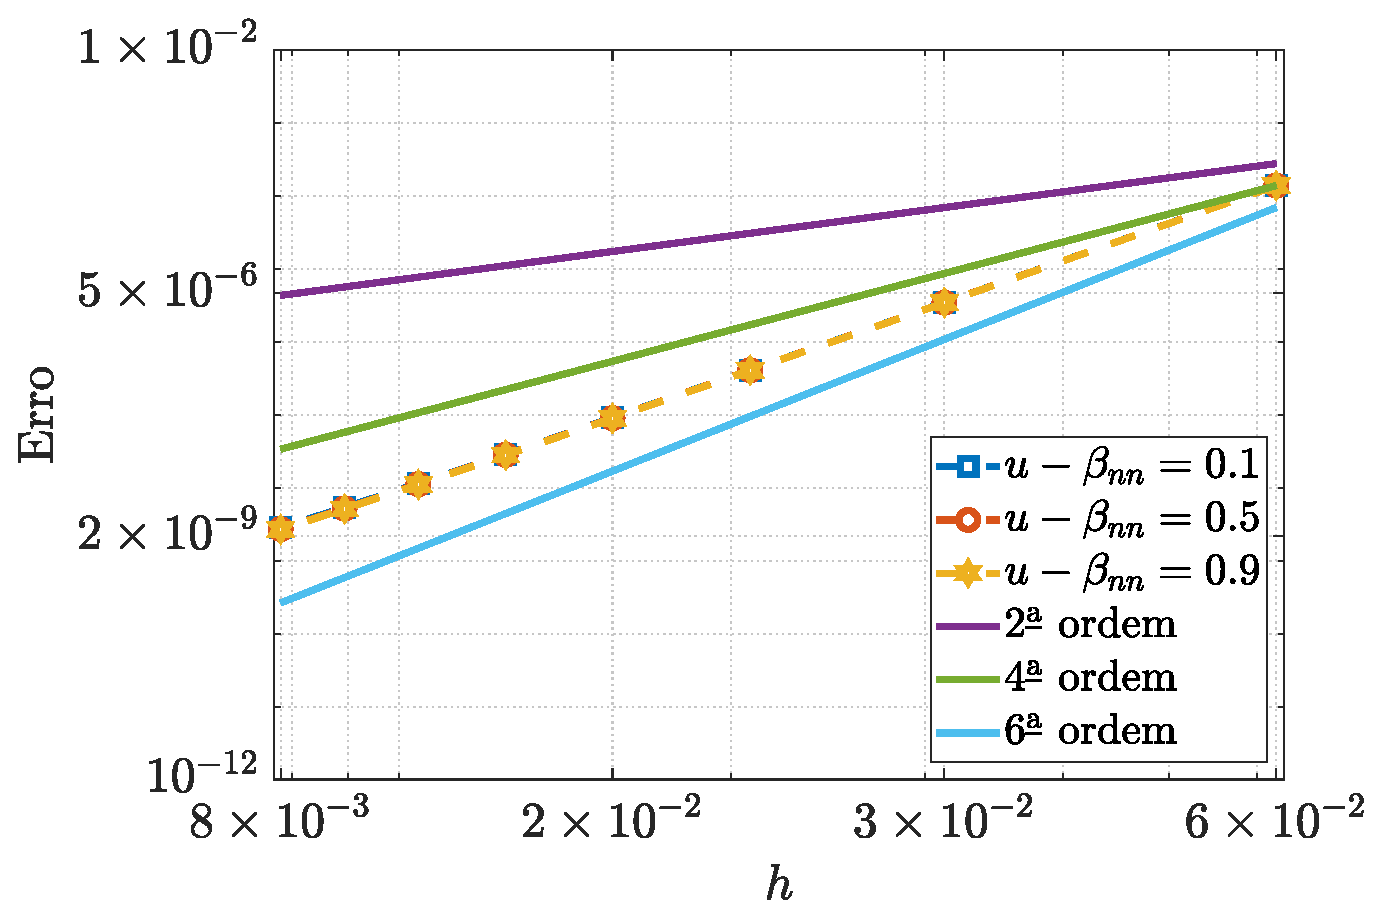
\includegraphics[width=\textwidth]{figures/Case12/OldroydB/Errors/NormErr_2nd_Re_100_Wi_1_epsilon_0_xi_0_alphaG_0_Dt_1e-06_at_0.05_tipsim_1_MMS_12_U.eps}
            \caption{$||U - \overline{u}||_{2}$}
            \label{error_u_2nd_Case1_oldorydb}
        \end{subfigure}
        \vspace{0.2cm}
        \qquad
        \begin{subfigure}[b]{.47\textwidth}
            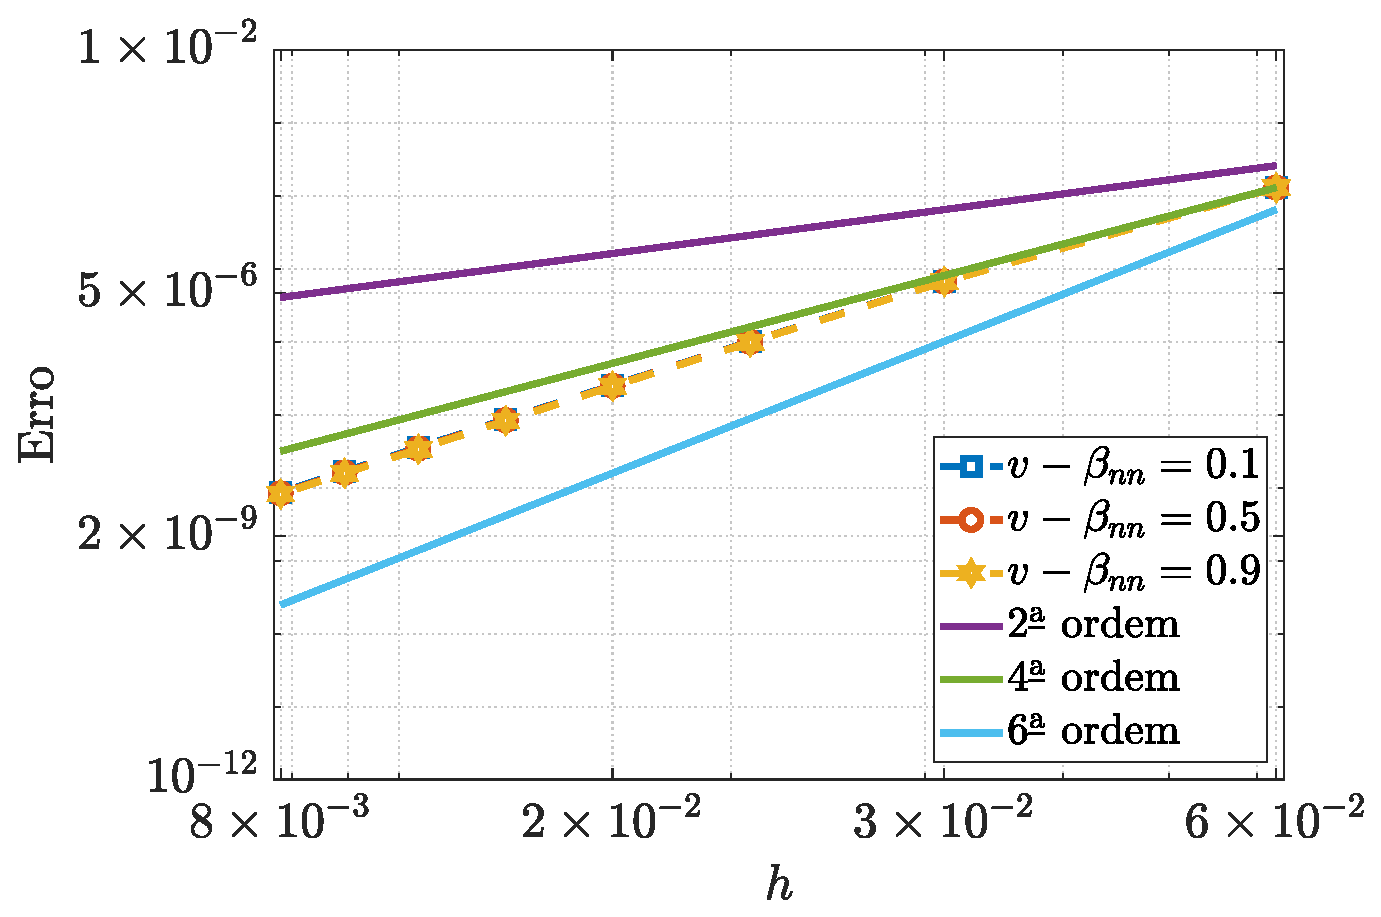
\includegraphics[width=\textwidth]{figures/Case12/OldroydB/Errors/NormErr_2nd_Re_100_Wi_1_epsilon_0_xi_0_alphaG_0_Dt_1e-06_at_0.05_tipsim_1_MMS_12_V.eps}
            \caption{$||V - \widetilde{v}||_{2}$}
            \label{error_v_2nd_Case1_oldorydb}
        \end{subfigure}
        \qquad
        \begin{subfigure}[b]{.47\textwidth}
            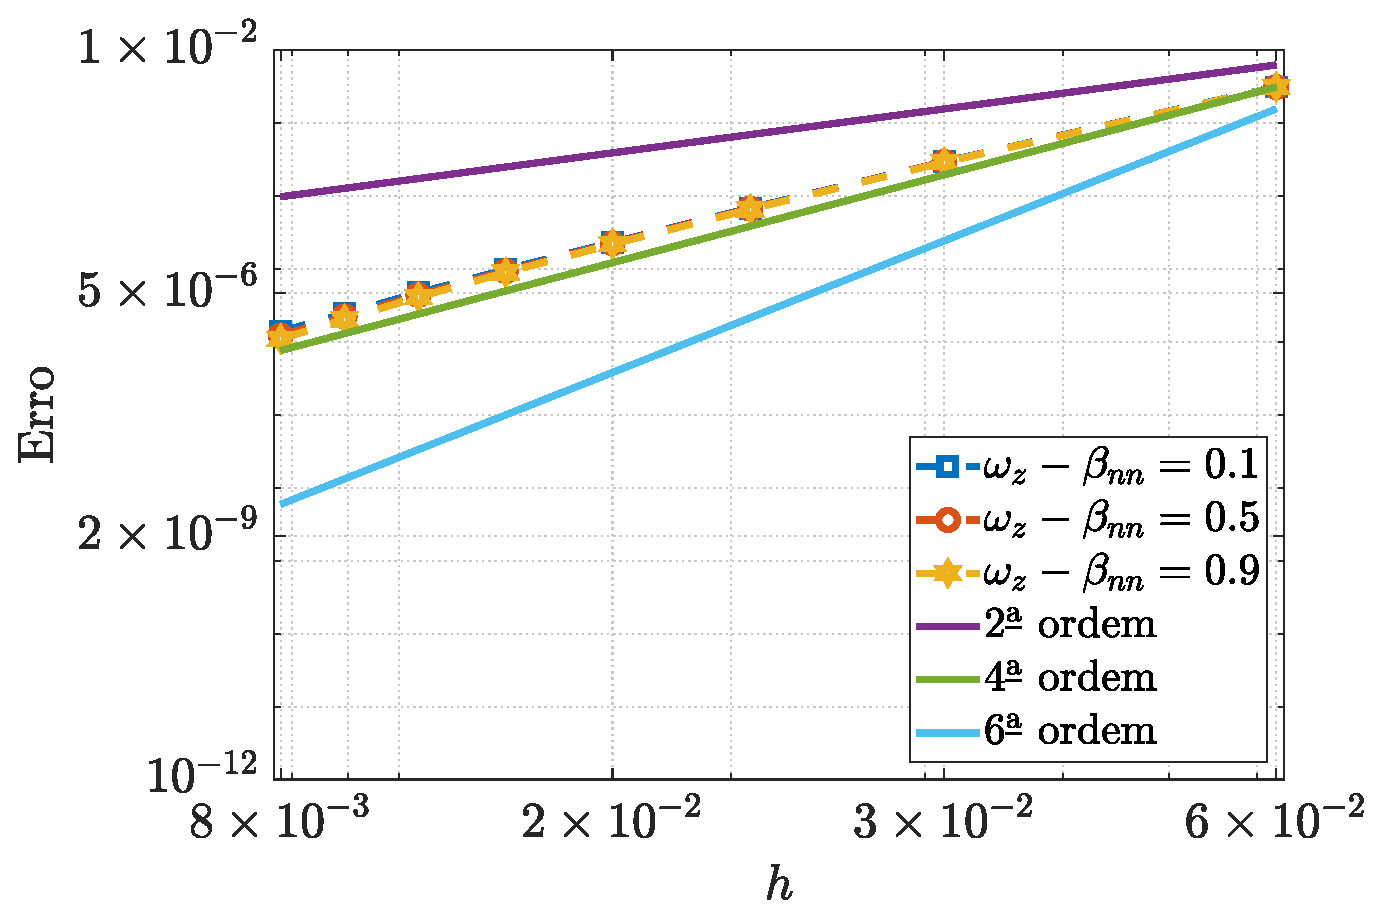
\includegraphics[width=\textwidth]{figures/Case12/OldroydB/Errors/NormErr_2nd_Re_100_Wi_1_epsilon_0_xi_0_alphaG_0_Dt_1e-06_at_0.05_tipsim_1_MMS_12_Wz.eps}
            \caption{$||\Omega_{z} - \widetilde{\omega_{z}}||_{2}$}
            \label{error_wz_2nd_Case1_oldorydb}
        \end{subfigure}
        \vspace{0.02cm}
        \qquad
        \begin{subfigure}[b]{.47\textwidth}
            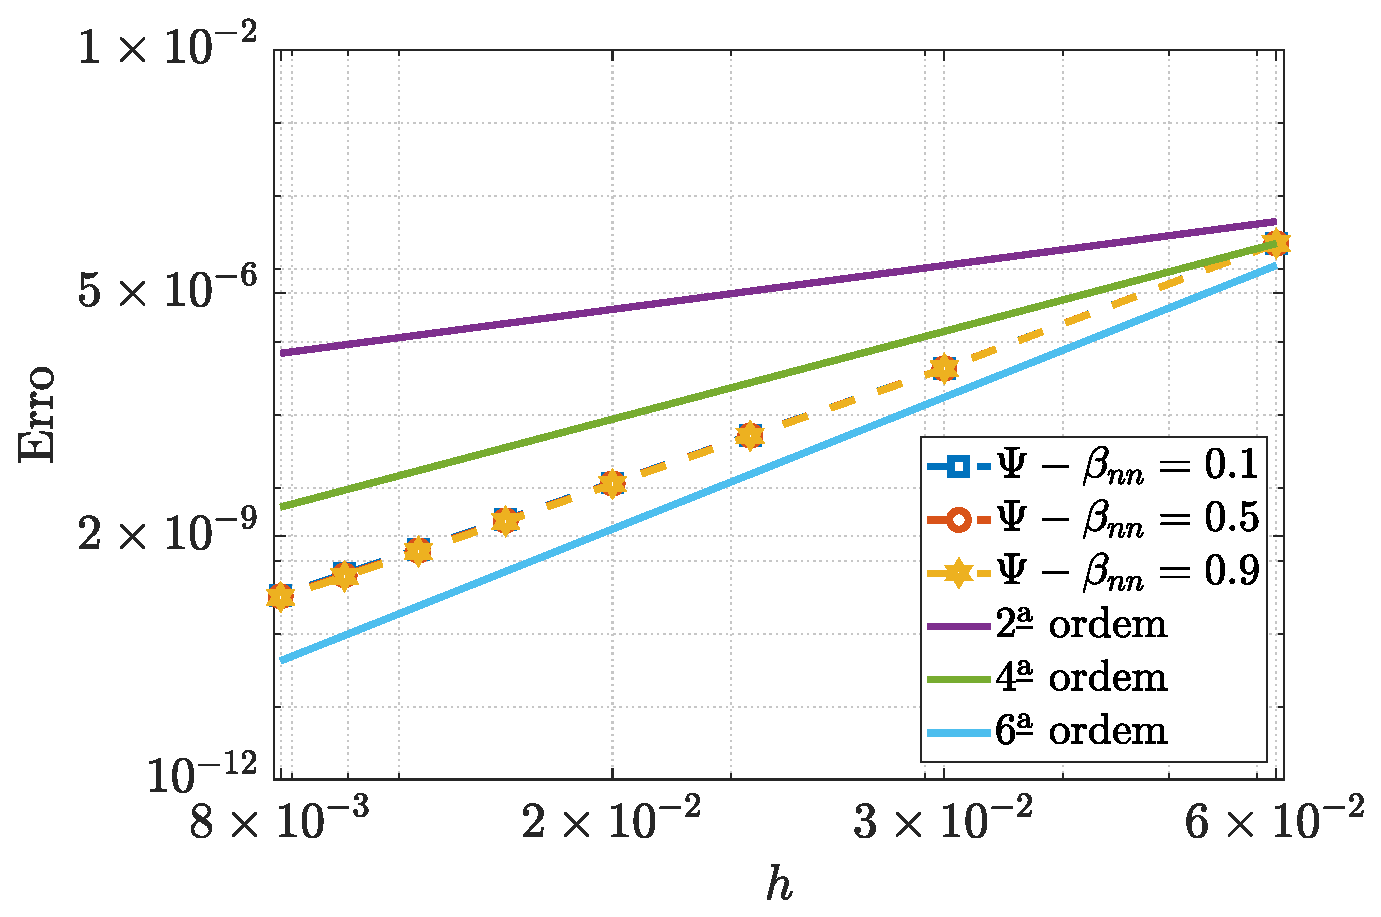
\includegraphics[width=\textwidth]{figures/Case12/OldroydB/Errors/NormErr_2nd_Re_100_Wi_1_epsilon_0_xi_0_alphaG_0_Dt_1e-06_at_0.05_tipsim_1_MMS_12_Psi.eps}
            \caption{$||\Psi - \widetilde{\Psi}||_{2}$}
            \label{error_psi_2nd_Case1_oldorydb}
        \end{subfigure}
        \fdadospesquisa
\end{figure}

\begin{figure}[H]
    \centering
    \caption{Erro para as componentes dos tensores de tensões, utilizando os parâmetros $Re=100$ e $Wi=1$, para o escoamento de fluido viscoelástico com o modelo Oldroyd-B}
    \label{OBerror2}
    \begin{subfigure}[b]{.47\textwidth}
        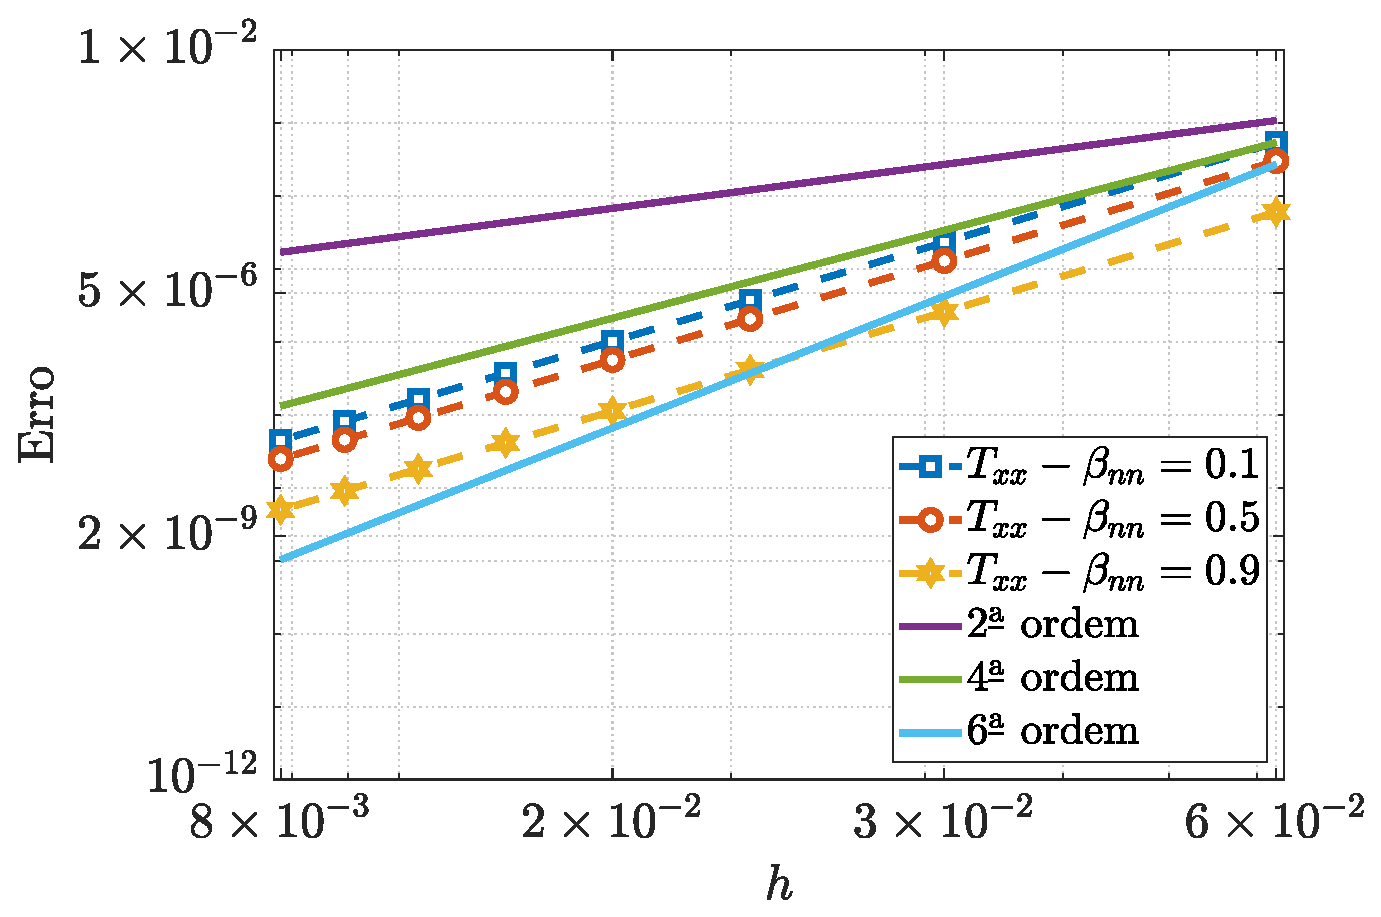
\includegraphics[width=\textwidth]{figures/Case12/OldroydB/Errors/NormErr_2nd_Re_100_Wi_1_epsilon_0_xi_0_alphaG_0_Dt_1e-06_at_0.05_tipsim_1_MMS_12_Txx.eps}
        \caption{$||T_{xx} - \overline{T}_{xx}||_{2}$}
        \label{error_txx_2nd_Case1_oldorydb}
    \end{subfigure}
    \vspace{0.2cm}
    \qquad
    \begin{subfigure}[b]{.47\textwidth}
        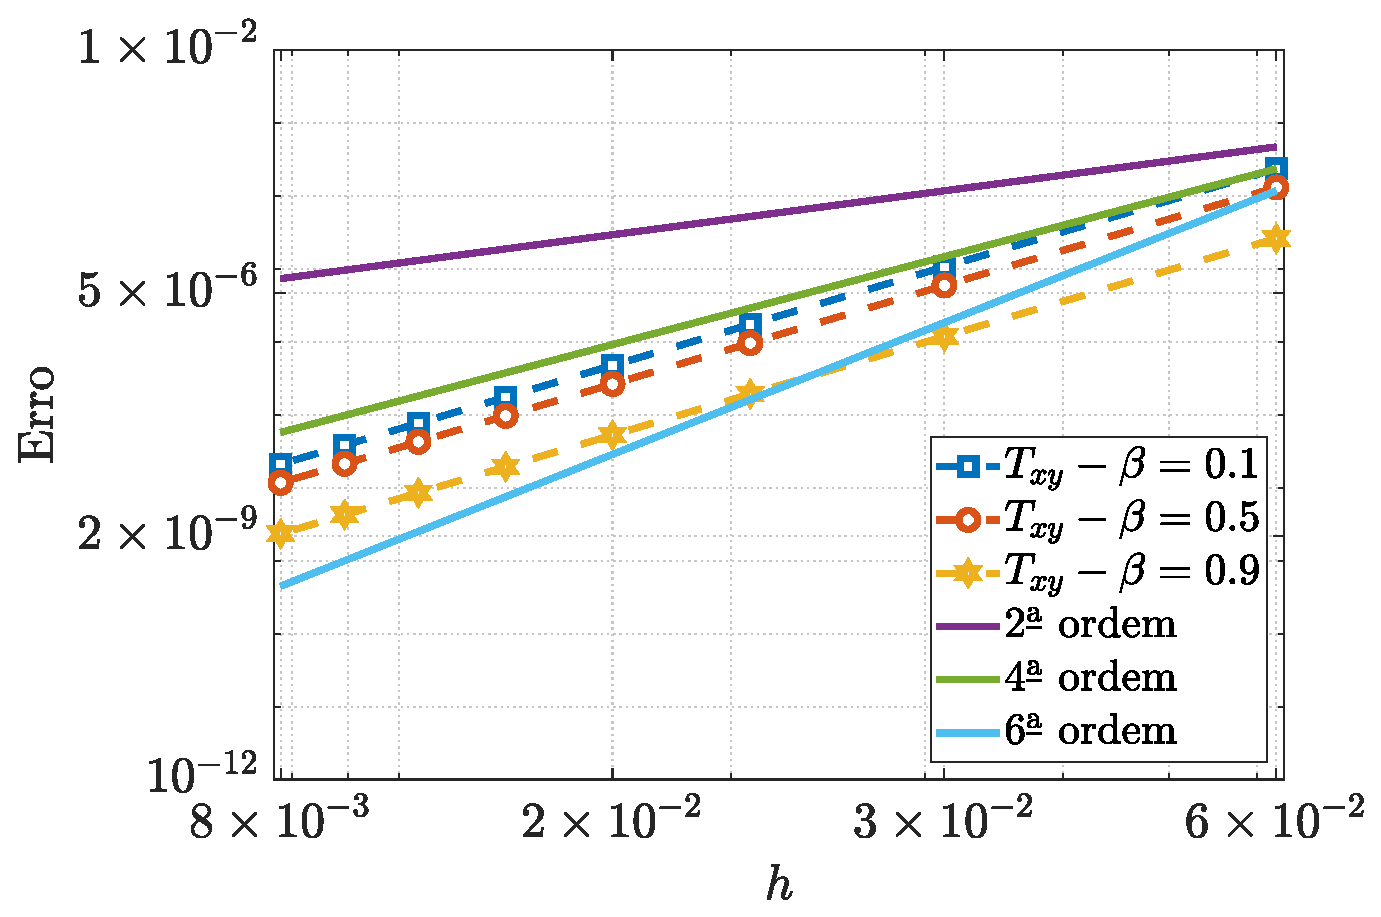
\includegraphics[width=\textwidth]{figures/Case12/OldroydB/Errors/NormErr_2nd_Re_100_Wi_1_epsilon_0_xi_0_alphaG_0_Dt_1e-06_at_0.05_tipsim_1_MMS_12_Txy.eps}
        \caption{$||T_{xy} - \overline{T}_{xy}||_{2}$}
        \label{error_txy_2nd_Case1_oldorydb}
    \end{subfigure}
    \qquad
    \begin{subfigure}[b]{.47\textwidth}
        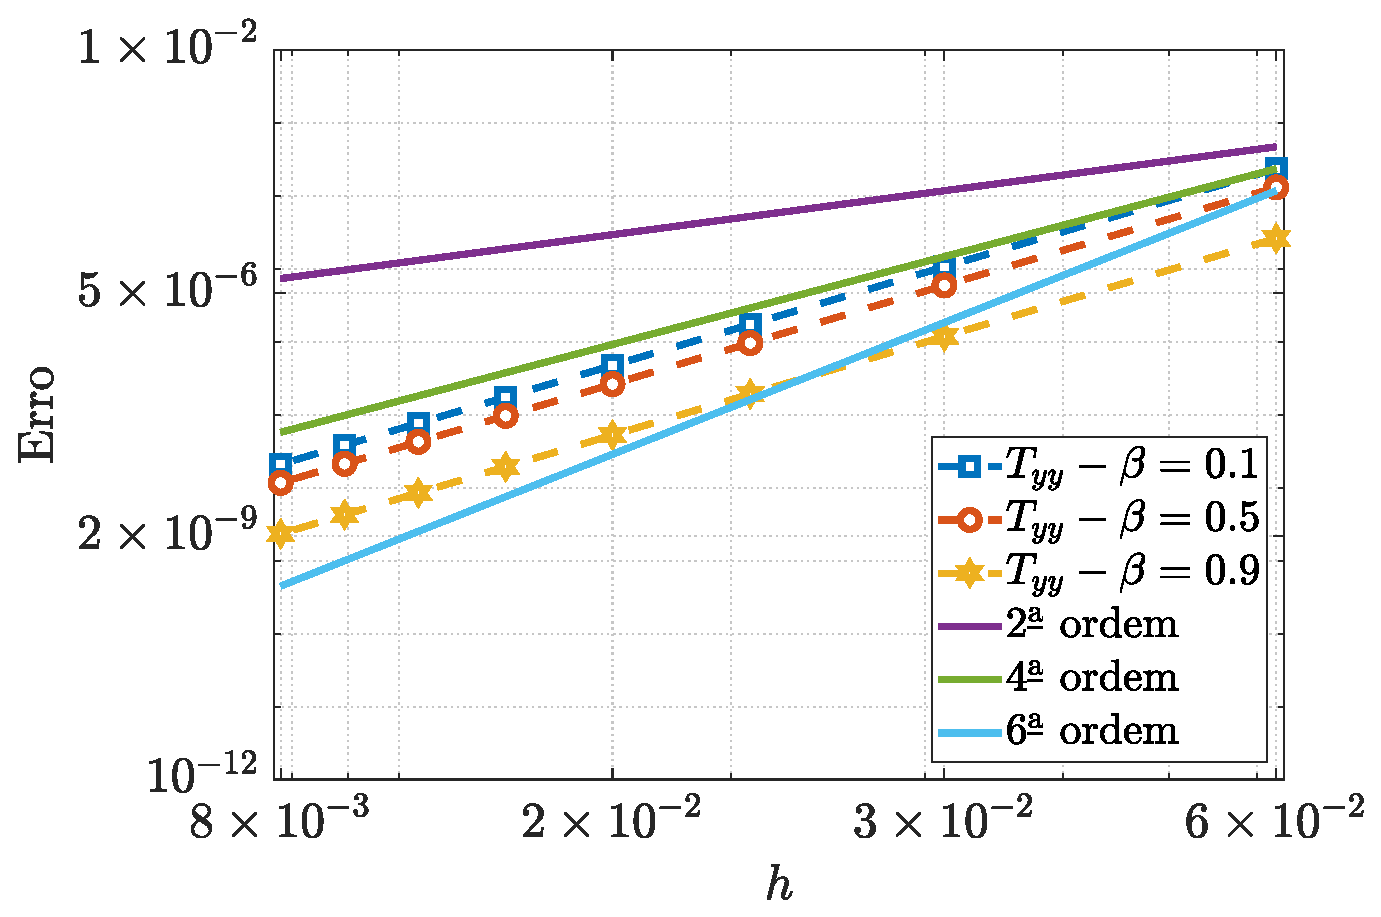
\includegraphics[width=\textwidth]{figures/Case12/OldroydB/Errors/NormErr_2nd_Re_100_Wi_1_epsilon_0_xi_0_alphaG_0_Dt_1e-06_at_0.05_tipsim_1_MMS_12_Tyy.eps}
        \caption{$||T_{yy} - \overline{T}_{yy}||_{2}$}
        \label{error_tyy_2nd_Case1_oldorydb}
    \end{subfigure}
    \fdadospesquisa
\end{figure}

As \autoref{OBerror1} e a \autoref{OBerror2} ilustram a ordem teórica de convergência obtida pelo código desenvolvido. Para proporcionar uma visão mais clara da convergência da vorticidade, a \autoref{tab_OldroydBWzResumida} apresenta os cálculos correspondentes para $Re = 1$, $100$, $400$, e $1000$, onde o comportamento discutido anteriormente pode ser claramente observado.
\begin{table}[H]
	\IBGEtab{
            \caption{Erros numéricos e cálculo da ordem de convergência para a vorticidade $(\omega_{z})$, utilizando o parâmetro $Wi=1$, para o escoamento de fluido viscoelástico Oldroyd-B}
            \label{tab_OldroydBWzResumida}
		}{
            \begin{tabular*}{\textwidth}{@{\extracolsep\fill}c|c|cc|cc|cc|cc@{}}
                \toprule
                 \multirow{2}{*}{$Re$} & \multirow{2}{*}{Malha} & \multicolumn{2}{c}{$\beta_{nn}=0.1$}  & \multicolumn{2}{c}{$\beta_{nn}=0.5$}  & \multicolumn{2}{c}{$\beta_{nn}=0.9$}  & \multicolumn{2}{c}{$\beta_{nn}=1.0$}\\ \cline{3-10}
                     & & Erro & p & Erro & p & Erro & p & Erro & p \\ \midrule
                    \multirow{7}{*}{1.00} & $17\times 17$ & 2.23e-03 & --- & 2.08e-03 & --- & 1.96e-03 & --- & 1.93e-03 & --- \\
                    & $33\times 33$ & 2.02e-04 & 3.47 & 1.51e-04 & 3.79 & 1.23e-04 & 4.00 & 1.18e-04 & 4.03 \\
                    & $49\times 49$ & 4.26e-05 & 3.84 & 2.50e-05 & 4.44 & 1.92e-05 & 4.57 & 1.84e-05 & 4.58 \\
                    & $65\times 65$ & 1.28e-05 & 4.17 & 6.43e-06 & 4.71 & 5.05e-06 & 4.65 & 4.85e-06 & 4.63 \\
                    & $81\times 81$ & 4.68e-06 & 4.52 & 2.23e-06 & 4.74 & 1.79e-06 & 4.63 & 1.73e-06 & 4.61 \\
                    & $97\times 97$ & 1.92e-06 & 4.90 & 9.34e-07 & 4.78 & 7.68e-07 & 4.65 & 7.45e-07 & 4.63 \\
                    & $113\times 113$ & 8.58e-07 & 5.21 & 4.47e-07 & 4.77 & 3.80e-07 & 4.57 & 3.71e-07 & 4.52 \\
                    & $129\times 129$ & 4.34e-07 & 5.10 & 2.59e-07 & 4.11 & 2.30e-07 & 3.76 & 2.26e-07 & 3.71 \\
                    \midrule
                    \multirow{7}{*}{100.00} & $17\times 17$ & 2.27e-03 & --- & 2.27e-03 & --- & 2.26e-03 & --- & 2.26e-03 & --- \\
                    & $33\times 33$ & 2.20e-04 & 3.37 & 2.19e-04 & 3.37 & 2.18e-04 & 3.37 & 2.18e-04 & 3.37 \\
                    & $49\times 49$ & 5.20e-05 & 3.56 & 5.15e-05 & 3.57 & 5.11e-05 & 3.58 & 5.10e-05 & 3.59 \\
                    & $65\times 65$ & 1.82e-05 & 3.66 & 1.79e-05 & 3.68 & 1.76e-05 & 3.70 & 1.75e-05 & 3.71 \\
                    & $81\times 81$ & 7.84e-06 & 3.76 & 7.65e-06 & 3.80 & 7.47e-06 & 3.84 & 7.43e-06 & 3.85 \\
                    & $97\times 97$ & 3.83e-06 & 3.93 & 3.70e-06 & 3.99 & 3.57e-06 & 4.05 & 3.54e-06 & 4.06 \\
                    & $113\times 113$ & 2.04e-06 & 4.10 & 1.94e-06 & 4.19 & 1.85e-06 & 4.27 & 1.83e-06 & 4.29 \\
                    & $129\times 129$ & 1.21e-06 & 3.89 & 1.13e-06 & 4.02 & 1.07e-06 & 4.13 & 1.05e-06 & 4.16 \\
                    \midrule
                    \multirow{7}{*}{400.00} & $17\times 17$ & 2.27e-03 & --- & 2.27e-03 & --- & 2.27e-03 & --- & 2.27e-03 & --- \\
                    & $33\times 33$ & 2.20e-04 & 3.37 & 2.20e-04 & 3.37 & 2.20e-04 & 3.37 & 2.20e-04 & 3.37 \\
                    & $49\times 49$ & 5.21e-05 & 3.56 & 5.19e-05 & 3.56 & 5.18e-05 & 3.56 & 5.18e-05 & 3.56 \\
                    & $65\times 65$ & 1.82e-05 & 3.65 & 1.81e-05 & 3.66 & 1.81e-05 & 3.66 & 1.81e-05 & 3.66 \\
                    & $81\times 81$ & 7.88e-06 & 3.75 & 7.83e-06 & 3.76 & 7.79e-06 & 3.77 & 7.78e-06 & 3.77 \\
                    & $97\times 97$ & 3.86e-06 & 3.92 & 3.83e-06 & 3.93 & 3.80e-06 & 3.94 & 3.79e-06 & 3.95 \\
                    & $113\times 113$ & 2.05e-06 & 4.09 & 2.03e-06 & 4.11 & 2.01e-06 & 4.12 & 2.01e-06 & 4.13 \\
                    & $129\times 129$ & 1.23e-06 & 3.86 & 1.21e-06 & 3.89 & 1.19e-06 & 3.92 & 1.19e-06 & 3.93 \\
                    \midrule
                    \multirow{7}{*}{1000.00} & $17\times 17$ & 2.27e-03 & --- & 2.27e-03 & --- & 2.27e-03 & --- & 2.27e-03 & --- \\
                    & $33\times 33$ & 2.20e-04 & 3.37 & 2.20e-04 & 3.37 & 2.20e-04 & 3.37 & 2.20e-04 & 3.37 \\
                    & $49\times 49$ & 5.21e-05 & 3.56 & 5.20e-05 & 3.56 & 5.20e-05 & 3.56 & 5.20e-05 & 3.56 \\
                    & $65\times 65$ & 1.82e-05 & 3.65 & 1.82e-05 & 3.65 & 1.82e-05 & 3.65 & 1.82e-05 & 3.65 \\
                    & $81\times 81$ & 7.89e-06 & 3.75 & 7.87e-06 & 3.76 & 7.86e-06 & 3.76 & 7.85e-06 & 3.76 \\
                    & $97\times 97$ & 3.86e-06 & 3.92 & 3.85e-06 & 3.92 & 3.84e-06 & 3.92 & 3.84e-06 & 3.92 \\
                    & $113\times 113$ & 2.06e-06 & 4.08 & 2.05e-06 & 4.09 & 2.04e-06 & 4.09 & 2.04e-06 & 4.09 \\
                    & $129\times 129$ & 1.23e-06 & 3.86 & 1.22e-06 & 3.87 & 1.22e-06 & 3.87 & 1.22e-06 & 3.88 \\
                    \bottomrule
                \end{tabular*}
		}{
		\fdadospesquisa
	}
\end{table}

Na \autoref{tab_OldroydBWzResumida}, os erros de vorticidade são apresentados para números de Reynolds ($Re$) iguais a 1, 100, 400 e 1000, considerando diferentes razões de viscosidade do solvente ($\beta_{nn} = 0.1,\ 0.5,\ 0.9$ e $1$). À medida que a malha é refinada, os erros diminuem consistentemente, com a ordem de convergência $p$ aproximando-se de 4.5, como esperado para métodos numéricos de alta ordem. A consistência na taxa de convergência para todos os números de Reynolds e razões de viscosidade reforça a precisão e a robustez do modelo.
\begin{table}[H]
	\IBGEtab{
            \caption{Erros numéricos e cálculo da ordem de convergência para a componente do tensor de tensões $T_{xx}$, utilizando o parâmetro $Wi=1$, para o escoamento de fluido viscoelástico Oldroyd-B}
            \label{tab_OldroydBTxxResumida}
		}{
		\begin{tabular*}{\textwidth}{@{\extracolsep\fill}c|c|cc|cc|cc|cc@{}}
                \toprule
                \multirow{2}{*}{$Re$} & \multirow{2}{*}{Malha} & \multicolumn{2}{c}{$\beta_{nn}=0.1$}  & \multicolumn{2}{c}{$\beta_{nn}=0.5$}  & \multicolumn{2}{c}{$\beta_{nn}=0.9$}  & \multicolumn{2}{c}{$\beta_{nn}=1.0$}  \\
                \cline{3-10}
                 & & Erro & p & Erro & p & Erro & p & Erro & p \\ \midrule
                \multirow{10}{*}{1.00} & 17$\times$17 & 5.38e-04 & --- & 2.99e-04 & --- & 5.97e-05 & --- & 5.97e-18 & --- \\
                & 33$\times$33 & 2.30e-05 & 4.54 & 1.28e-05 & 4.54 & 2.56e-06 & 4.54 & 2.56e-19 & 4.54 \\
                & 49$\times$49 & 3.69e-06 & 4.52 & 2.05e-06 & 4.52 & 4.10e-07 & 4.52 & 4.10e-20 & 4.52 \\
                & 65$\times$65 & 1.01e-06 & 4.51 & 5.61e-07 & 4.51 & 1.12e-07 & 4.51 & 1.12e-20 & 4.51 \\
                & 81$\times$81 & 3.69e-07 & 4.50 & 2.05e-07 & 4.50 & 4.10e-08 & 4.50 & 4.10e-21 & 4.50 \\
                & 97$\times$97 & 1.62e-07 & 4.50 & 9.03e-08 & 4.50 & 1.80e-08 & 4.50 & 1.80e-21 & 4.50 \\
                & 113$\times$113 & 8.12e-08 & 4.50 & 4.51e-08 & 4.50 & 9.02e-09 & 4.50 & 9.01e-22 & 4.50 \\
                & 129$\times$129 & 4.45e-08 & 4.50 & 2.47e-08 & 4.50 & 4.94e-09 & 4.50 & 4.94e-22 & 4.50 \\
                \midrule
                \multirow{10}{*}{100.00} & 17$\times$17 & 5.38e-04 & --- & 2.99e-04 & --- & 5.97e-05 & --- & 5.97e-18 & --- \\
                & 33$\times$33 & 2.30e-05 & 4.54 & 1.28e-05 & 4.54 & 2.56e-06 & 4.54 & 2.56e-19 & 4.54 \\
                & 49$\times$49 & 3.69e-06 & 4.52 & 2.05e-06 & 4.52 & 4.10e-07 & 4.52 & 4.10e-20 & 4.52 \\
                & 65$\times$65 & 1.01e-06 & 4.51 & 5.61e-07 & 4.51 & 1.12e-07 & 4.51 & 1.12e-20 & 4.51 \\
                & 81$\times$81 & 3.69e-07 & 4.50 & 2.05e-07 & 4.50 & 4.10e-08 & 4.50 & 4.10e-21 & 4.50 \\
                & 97$\times$97 & 1.62e-07 & 4.50 & 9.03e-08 & 4.50 & 1.81e-08 & 4.50 & 1.80e-21 & 4.50 \\
                & 113$\times$113 & 8.12e-08 & 4.50 & 4.51e-08 & 4.50 & 9.02e-09 & 4.50 & 9.01e-22 & 4.50 \\
                & 129$\times$129 & 4.45e-08 & 4.50 & 2.47e-08 & 4.50 & 4.94e-09 & 4.50 & 4.94e-22 & 4.50 \\
                \midrule
                \multirow{10}{*}{400.00} & 17$\times$17 & 5.38e-04 & --- & 2.99e-04 & --- & 5.97e-05 & --- & 5.97e-18 & --- \\
                & 33$\times$33 & 2.30e-05 & 4.54 & 1.28e-05 & 4.54 & 2.56e-06 & 4.54 & 2.56e-19 & 4.54 \\
                & 49$\times$49 & 3.69e-06 & 4.52 & 2.05e-06 & 4.52 & 4.10e-07 & 4.52 & 4.10e-20 & 4.52 \\
                & 65$\times$65 & 1.01e-06 & 4.51 & 5.61e-07 & 4.51 & 1.12e-07 & 4.51 & 1.12e-20 & 4.51 \\
                & 81$\times$81 & 3.69e-07 & 4.50 & 2.05e-07 & 4.50 & 4.10e-08 & 4.50 & 4.10e-21 & 4.50 \\
                & 97$\times$97 & 1.62e-07 & 4.50 & 9.03e-08 & 4.50 & 1.81e-08 & 4.50 & 1.80e-21 & 4.50 \\
                & 113$\times$113 & 8.11e-08 & 4.50 & 4.51e-08 & 4.50 & 9.02e-09 & 4.50 & 9.01e-22 & 4.50 \\
                & 129$\times$129 & 4.45e-08 & 4.50 & 2.47e-08 & 4.50 & 4.94e-09 & 4.50 & 4.94e-22 & 4.50 \\
                \midrule
                \multirow{10}{*}{1000.00} & 17$\times$17 & 5.38e-04 & --- & 2.99e-04 & --- & 5.97e-05 & --- & 5.97e-18 & --- \\
                & 33$\times$33 & 2.30e-05 & 4.54 & 1.28e-05 & 4.54 & 2.56e-06 & 4.54 & 2.56e-19 & 4.54 \\
                & 49$\times$49 & 3.69e-06 & 4.52 & 2.05e-06 & 4.52 & 4.10e-07 & 4.52 & 4.10e-20 & 4.52 \\
                & 65$\times$65 & 1.01e-06 & 4.51 & 5.61e-07 & 4.51 & 1.12e-07 & 4.51 & 1.12e-20 & 4.51 \\
                & 81$\times$81 & 3.69e-07 & 4.50 & 2.05e-07 & 4.50 & 4.10e-08 & 4.50 & 4.10e-21 & 4.50 \\
                & 97$\times$97 & 1.62e-07 & 4.50 & 9.03e-08 & 4.50 & 1.81e-08 & 4.50 & 1.80e-21 & 4.50 \\
                & 113$\times$113 & 8.11e-08 & 4.50 & 4.51e-08 & 4.50 & 9.02e-09 & 4.50 & 9.01e-22 & 4.50 \\
                & 129$\times$129 & 4.45e-08 & 4.50 & 2.47e-08 & 4.50 & 4.94e-09 & 4.50 & 4.94e-22 & 4.50 \\
                \bottomrule
            \end{tabular*}
		}{
		\fdadospesquisa
	}
\end{table}

A \autoref{tab_OldroydBTxxResumida} apresenta os erros e as ordens de convergência para o componente $T_{xx}$ do tensor de tensões extra. Similarmente aos resultados da vorticidade, observa-se uma redução clara nos erros à medida que a malha é refinada, com a ordem de convergência permanecendo próxima de 4.5 em todas as condições avaliadas. Esses resultados indicam a estabilidade e robustez do método numérico, tanto na simulação da vorticidade quanto nas tensões extras. Ao examinar a tabela, para $\beta_{nn} = 1$, fica evidente que os erros numéricos são extremamente pequenos, aproximando-se dos níveis de precisão de máquina (por exemplo, $5.97e-18$ ou $4.94e-22$). Esse comportamento é esperado, visto que $\beta_{nn} = 1$ corresponde ao caso de um fluido Newtoniano, onde os tensores de tensões extras como $T_{xx}$ se tornam aproximadamente nulos. Como resultado, os erros são mínimos e a ordem de convergência permanece consistentemente em torno de 4.5, alinhando-se com o desempenho esperado para métodos numéricos de alta ordem. Os erros quase nulos para $\beta_{nn} = 1$ demonstram que o esquema numérico captura com precisão o caso limite de um fluido Newtoniano.

\subsection{Caso de verificação usando o modelo Giesekus}

Nas simulações realizadas com o modelo de Giesekus, foram utilizados números de Reynolds variando de $Re = 1,\ 10,\ 100,\ 400$ e $1000$, com o número de Weissenberg mantido fixo em $Wi = 1$, e diferentes razões de viscosidade do solvente $\beta_{nn} = 0.1,\ 0.5,\ 0.9$ e $1$. Além disso, o parâmetro $\alpha_G$ foi ajustado para valores de $0.1$, $0.5$ e $0.85$, visando analisar o comportamento do modelo sob diferentes regimes de escoamento. A análise de erro foi conduzida para avaliar o desempenho do método em relação ao campo de velocidade, vorticidade, função de corrente e tensores de tensões extras.

Na \autoref{GEerror011}, são apresentados os gráficos de erro para os componentes do campo de velocidade, vorticidade e função de corrente, considerando o modelo de Giesekus com $Re = 100$, $Wi = 1$ e $\alpha_G = 0.1$. Como demonstrado, os erros diminuem consistentemente à medida que a malha é refinada. A ordem de convergência $p$ aproxima-se de 4.5, conforme esperado para métodos numéricos de alta ordem. Esse comportamento consistente reforça a robustez e a precisão do esquema numérico, demonstrando sua eficácia na captura das dinâmicas de fluidos viscoelásticos sob diferentes razões de viscosidade do solvente. Essa análise é fundamental para validar a capacidade do modelo em simular corretamente diferentes propriedades do escoamento.
\begin{figure}[H] 
    \centering
    \caption{Erro para o campo de velocidade $(\overline{u},\tilde{v})$, vorticidade $(\tilde{\omega_{z}})$ e função de corrente $(\tilde{\psi})$, considerando $Re=100$, $Wi=1$ e $\alpha_G=0.1$, para o escoamento de fluido viscoelástico com o modelo Giesekus}\label{GEerror011}
    \begin{subfigure}[b]{.47\textwidth}
        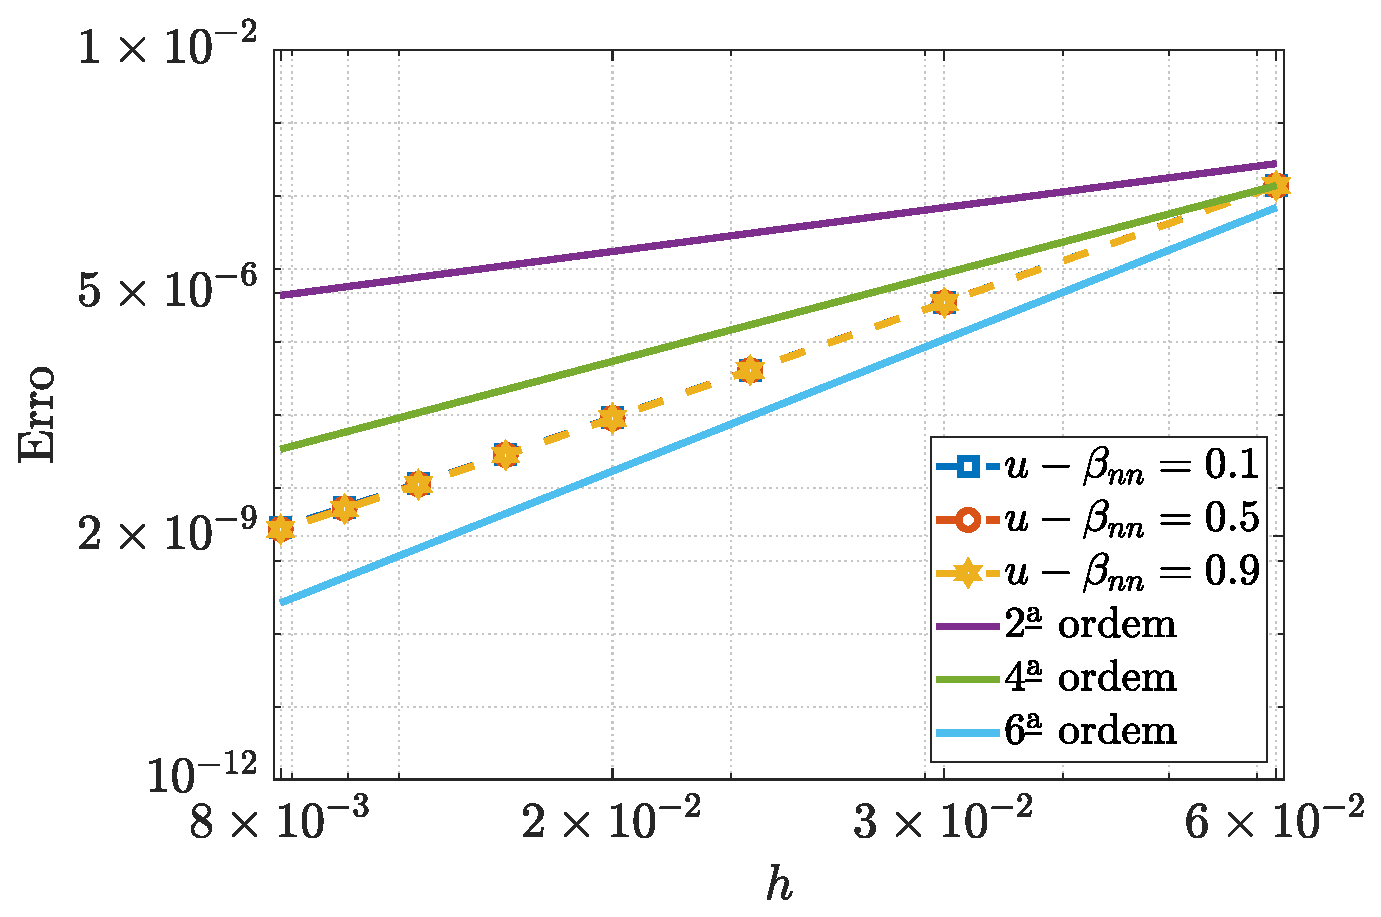
\includegraphics[width=\textwidth]{figures/Case12/Giesekus/Errors/NormErr_2nd_Re_100_Wi_1_epsilon_0_xi_0_alphaG_0.1_Dt_1e-06_at_0.05_tipsim_1_MMS_12_U.eps}
        \caption{$||U - \overline{u}||_{2}$}
        \label{error_u_2nd_Case1_giesekus_alphaG_0.1}
    \end{subfigure}
    \vspace{0.2cm}
    \qquad
    \begin{subfigure}[b]{.47\textwidth}
        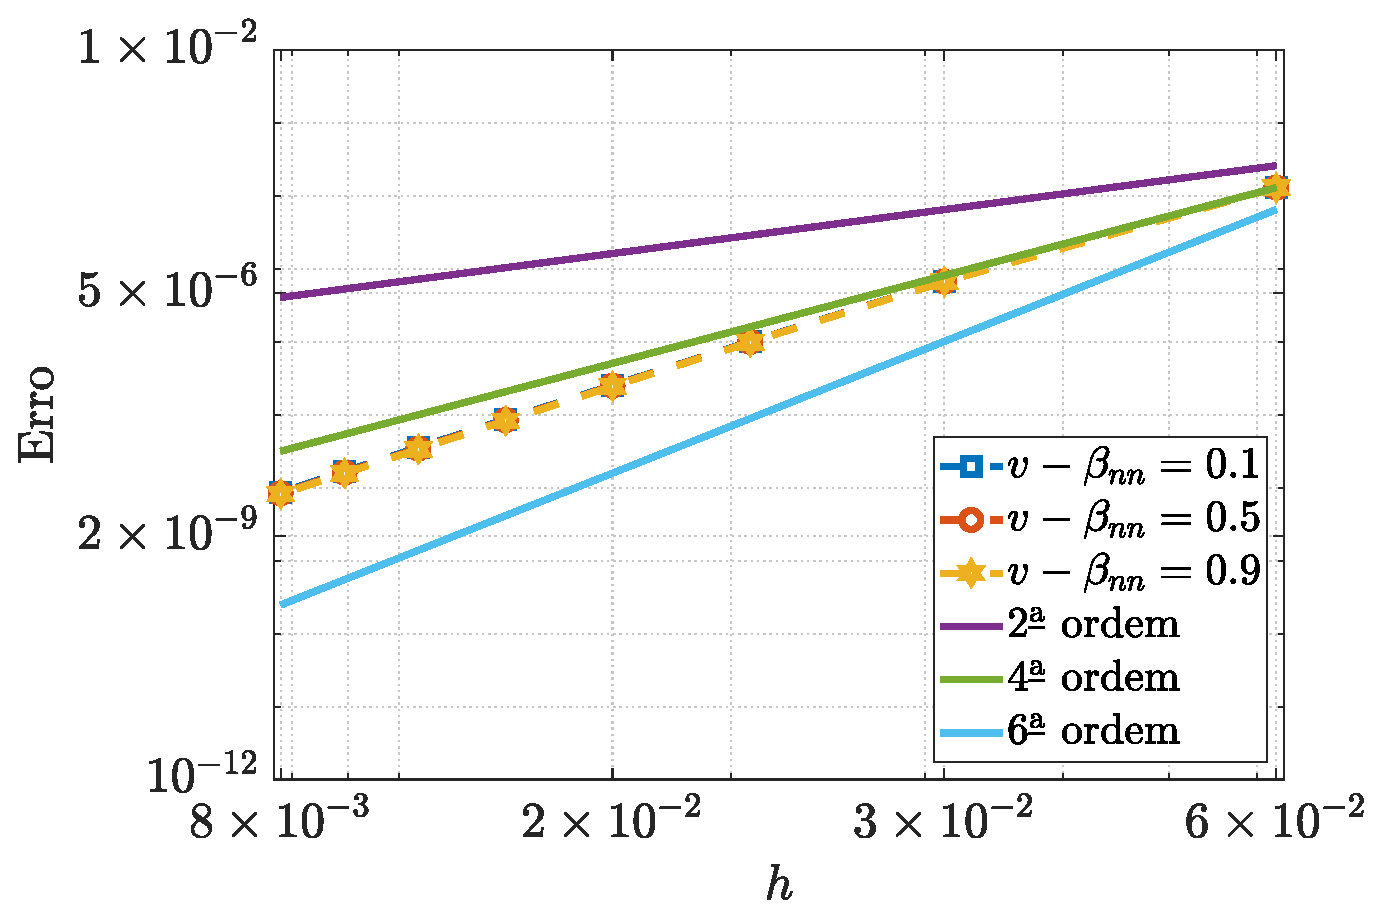
\includegraphics[width=\textwidth]{figures/Case12/Giesekus/Errors/NormErr_2nd_Re_100_Wi_1_epsilon_0_xi_0_alphaG_0.1_Dt_1e-06_at_0.05_tipsim_1_MMS_12_V.eps}
        \caption{$||V - \widetilde{v}||_{2}$}
        \label{error_v_2nd_Case1_giesekus_alphaG_0.1}
    \end{subfigure}
    \qquad
    \begin{subfigure}[b]{.47\textwidth}
        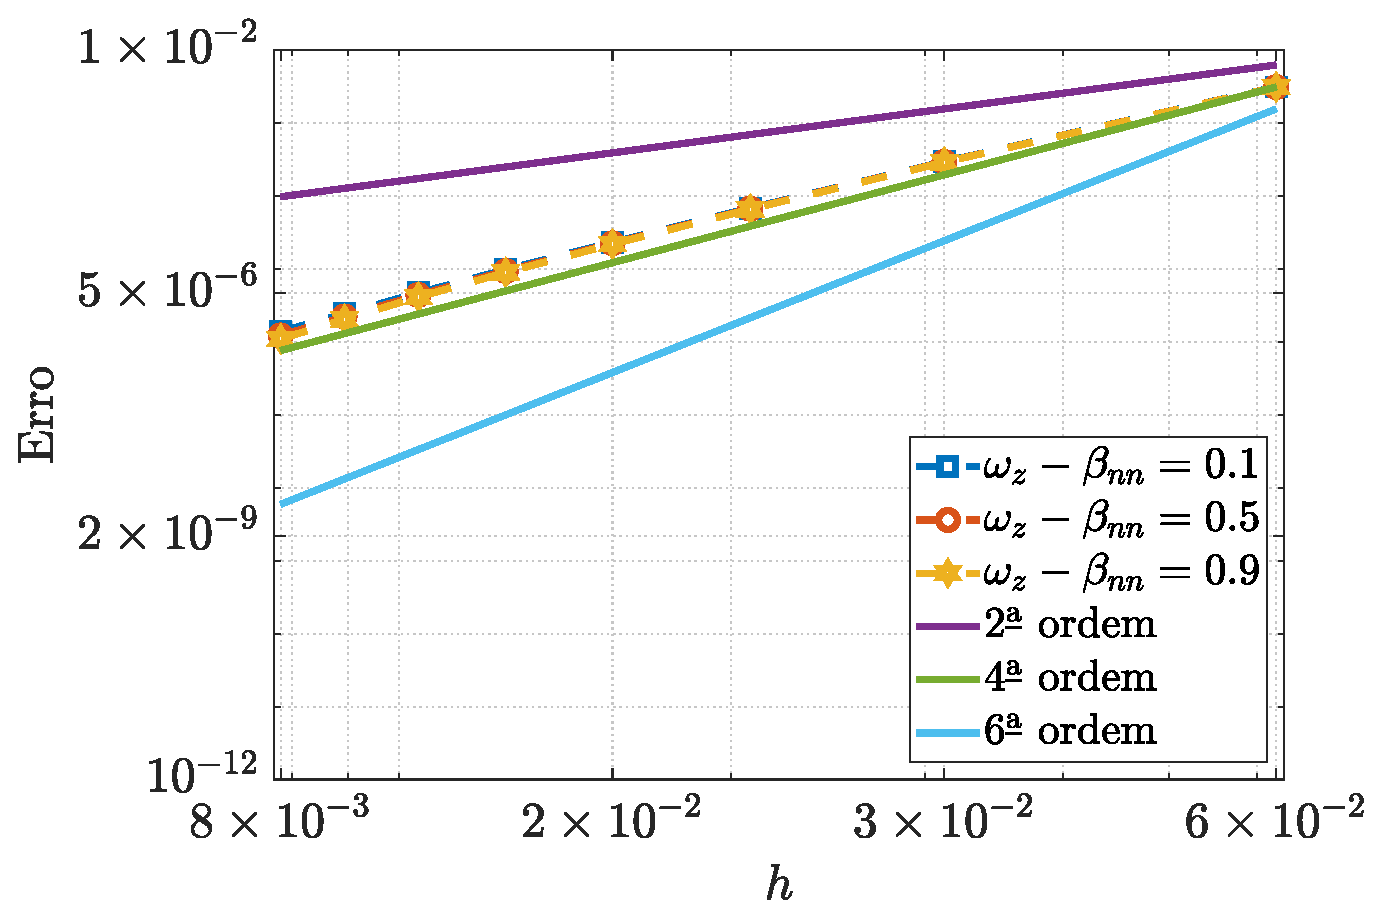
\includegraphics[width=\textwidth]{figures/Case12/Giesekus/Errors/NormErr_2nd_Re_100_Wi_1_epsilon_0_xi_0_alphaG_0.1_Dt_1e-06_at_0.05_tipsim_1_MMS_12_Wz.eps}
        \caption{$||\Omega_{z} - \widetilde{\omega_{z}}||_{2}$}
        \label{error_wz_2nd_Case1_giesekus_alphaG_0.1}
    \end{subfigure}
    \qquad
    \begin{subfigure}[b]{.47\textwidth}
        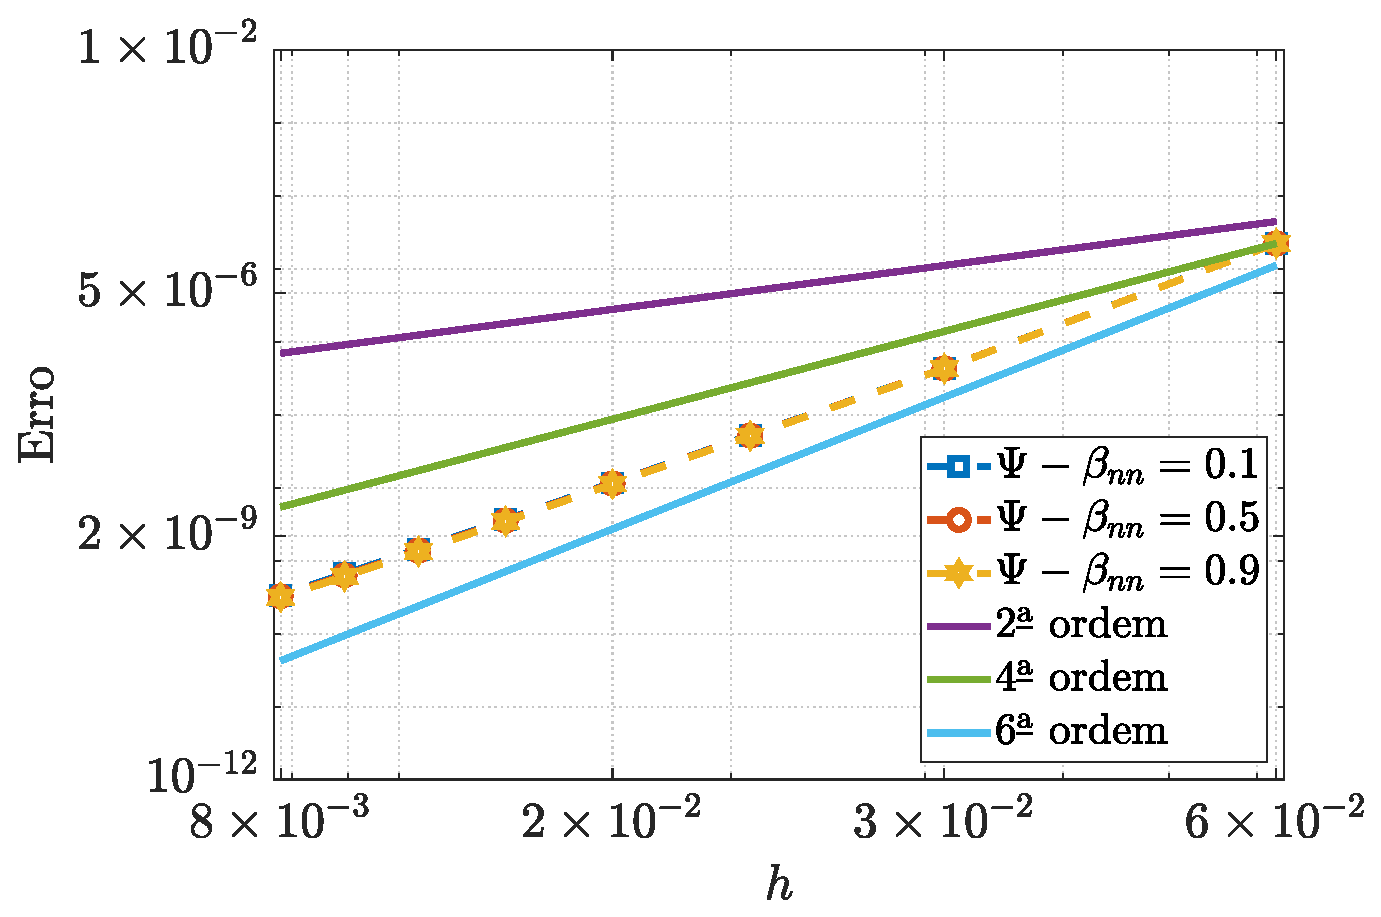
\includegraphics[width=\textwidth]{figures/Case12/Giesekus/Errors/NormErr_2nd_Re_100_Wi_1_epsilon_0_xi_0_alphaG_0.1_Dt_1e-06_at_0.05_tipsim_1_MMS_12_Psi.eps}
        \caption{$||\Psi - \widetilde{\Psi}||_{2}$}
        \label{error_psi_2nd_Case1_oldorydbgiesekus_alphaG_0.1}
    \end{subfigure}
    \fautor
\end{figure}

A \autoref{GEerror012} amplia a análise ao apresentar os erros relacionados à conformidade dos tensores extra-tensões $T_{xx}$, $T_{xy}$ e $T_{yy}$, para o mesmo conjunto de parâmetros $Re = 100$, $Wi = 1$ e $\alpha_G = 0.1$. Os resultados indicam uma redução significativa nos erros à medida que a malha é refinada, mantendo uma alta ordem de convergência, geralmente próxima de 4,5. Isso sugere que o método numérico é robusto na captura da complexidade das tensões extras em fluidos viscoelásticos, minimizando as discrepâncias para diferentes valores de $\beta_{nn}$.
\begin{figure}[H]
    \centering
    \caption{Erro para os componentes tensores extra-tensão, usando os parâmetros $Re=100,$ $Wi=1$ e $\alpha_{G} = 0.1$, para o fluxo de fluido viscoelástico com o modelo Giesekus}\label{GEerror012}
    \begin{subfigure}[b]{.47\textwidth}
        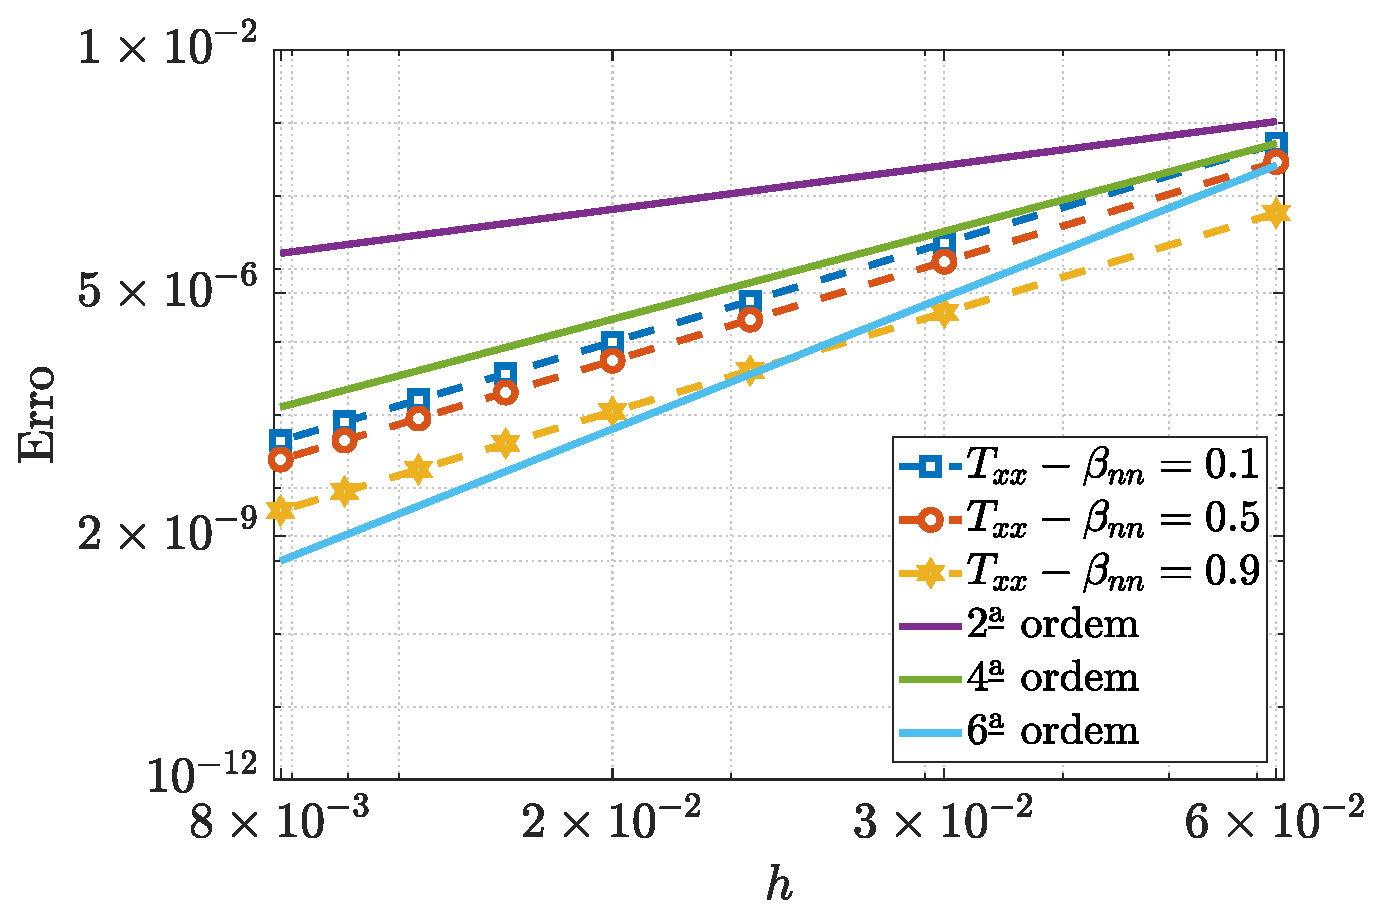
\includegraphics[width=\textwidth]{figures/Case12/Giesekus/Errors/NormErr_2nd_Re_100_Wi_1_epsilon_0_xi_0_alphaG_0.1_Dt_1e-06_at_0.05_tipsim_1_MMS_12_Txx.eps}
        \caption{$||T_{xx} - \overline{T}_{xx}||_{2}$}
        \label{error_txx_2nd_Case1_giesekus_alphaG_0.1}
    \end{subfigure}
    \vspace{0.2cm}
    \qquad
    \begin{subfigure}[b]{.47\textwidth}
        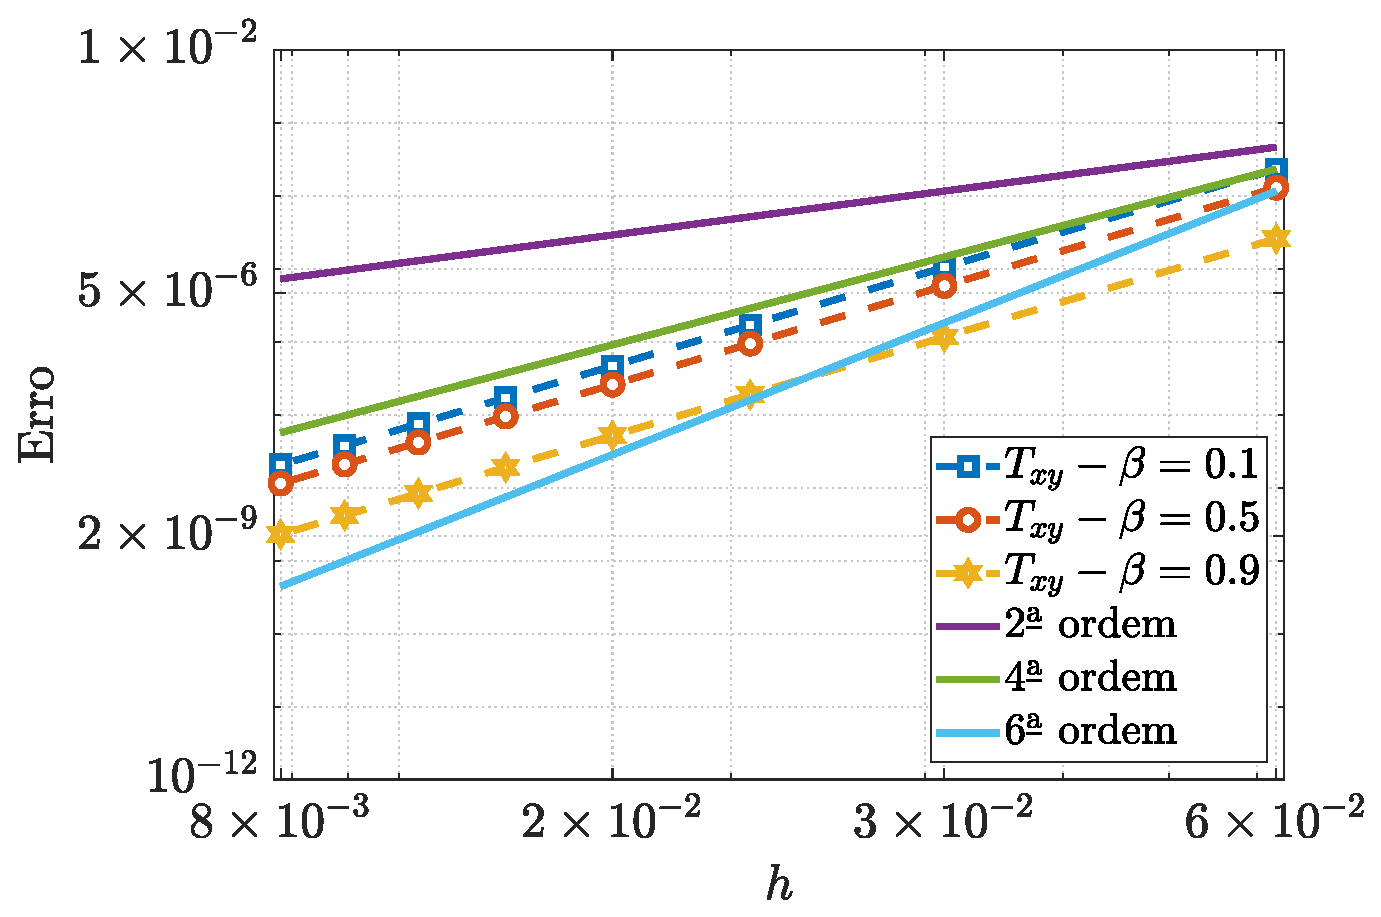
\includegraphics[width=\textwidth]{figures/Case12/Giesekus/Errors/NormErr_2nd_Re_100_Wi_1_epsilon_0_xi_0_alphaG_0.1_Dt_1e-06_at_0.05_tipsim_1_MMS_12_Txy.eps}
        \caption{$||T_{xy} - \overline{T}_{xy}||_{2}$}
        \label{error_txy_2nd_Case1_giesekus_alphaG_0.1}
    \end{subfigure}
    \qquad
    \begin{subfigure}[b]{.47\textwidth}
        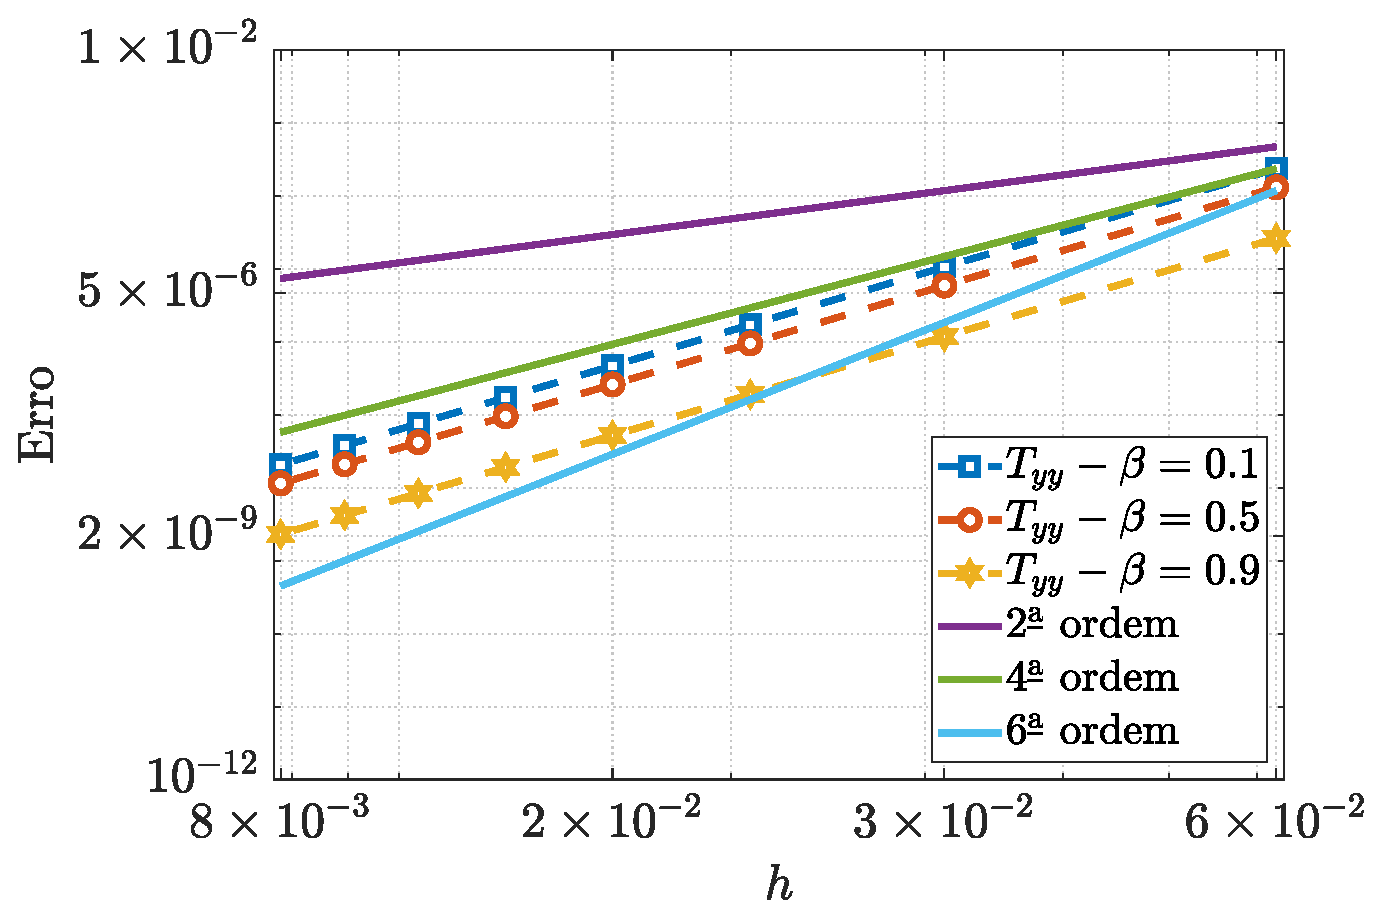
\includegraphics[width=\textwidth]{figures/Case12/Giesekus/Errors/NormErr_2nd_Re_100_Wi_1_epsilon_0_xi_0_alphaG_0.1_Dt_1e-06_at_0.05_tipsim_1_MMS_12_Tyy.eps}
        \caption{$||T_{yy} - \overline{T}_{yy}||_{2}$}
        \label{error_tyy_2nd_Case1_giesekus_alphaG_0.1}
    \end{subfigure}
    \fautor
\end{figure}

\begin{table}[H]
	\IBGEtab{
		\caption{Erros numéricos e cálculo da ordem de convergência para $\omega_{z}$, usando os parâmetros $Wi = 1$ e $\alpha_G = 0.1$, para o fluxo de fluido viscoelástico de Giesekus}\label{tab_GiesekusWzalphaG01Resumida}
	}{
		\begin{tabular*}{\textwidth}{@{\extracolsep\fill}c|c|cc|cc|cc|cc@{}}
                \toprule
                \multirow{2}{*}{$Re$} & \multirow{2}{*}{Malha} & \multicolumn{2}{c}{$\beta_{nn}=0.1$}  & \multicolumn{2}{c}{$\beta_{nn}=0.5$}  & \multicolumn{2}{c}{$\beta_{nn}=0.9$}  & \multicolumn{2}{c}{$\beta_{nn}=1.0$}  \\
                \cline{3-10}
                 & & Erro & p & Erro & p & Erro & p & Erro & p \\
                \midrule
                \multirow{10}{*}{1.00} & 17$\times$17 & 3.02e-03 & --- & 2.77e-03 & --- & 2.57e-03 & --- & 2.52e-03 & --- \\
                & 33$\times$33 & 2.54e-04 & 3.57 & 1.70e-04 & 4.03 & 1.35e-04 & 4.25 & 1.29e-04 & 4.29 \\
                & 49$\times$49 & 4.87e-05 & 4.07 & 2.59e-05 & 4.64 & 1.99e-05 & 4.72 & 1.90e-05 & 4.73 \\
                & 65$\times$65 & 1.32e-05 & 4.53 & 6.41e-06 & 4.85 & 4.91e-06 & 4.86 & 4.68e-06 & 4.86 \\
                & 81$\times$81 & 4.46e-06 & 4.87 & 2.14e-06 & 4.91 & 1.67e-06 & 4.84 & 1.60e-06 & 4.81 \\
                & 97$\times$97 & 1.76e-06 & 5.09 & 8.69e-07 & 4.95 & 6.98e-07 & 4.77 & 6.76e-07 & 4.72 \\
                & 113$\times$113 & 7.91e-07 & 5.20 & 4.11e-07 & 4.86 & 3.46e-07 & 4.55 & 3.38e-07 & 4.50 \\
                & 129$\times$129 & 4.07e-07 & 4.98 & 2.39e-07 & 4.05 & 2.14e-07 & 3.61 & 2.11e-07 & 3.54 \\
                \midrule
                \multirow{10}{*}{100.00} & 17$\times$17 & 3.10e-03 & --- & 3.09e-03 & --- & 3.08e-03 & --- & 3.08e-03 & --- \\
                & 33$\times$33 & 2.93e-04 & 3.40 & 2.91e-04 & 3.41 & 2.88e-04 & 3.42 & 2.88e-04 & 3.42 \\
                & 49$\times$49 & 6.76e-05 & 3.62 & 6.65e-05 & 3.64 & 6.54e-05 & 3.66 & 6.51e-05 & 3.66 \\
                & 65$\times$65 & 2.30e-05 & 3.75 & 2.23e-05 & 3.79 & 2.17e-05 & 3.83 & 2.16e-05 & 3.84 \\
                & 81$\times$81 & 9.72e-06 & 3.86 & 9.28e-06 & 3.93 & 8.88e-06 & 4.01 & 8.79e-06 & 4.02 \\
                & 97$\times$97 & 4.66e-06 & 4.03 & 4.36e-06 & 4.14 & 4.09e-06 & 4.25 & 4.03e-06 & 4.27 \\
                & 113$\times$113 & 2.42e-06 & 4.25 & 2.21e-06 & 4.41 & 2.03e-06 & 4.55 & 1.99e-06 & 4.58 \\
                & 129$\times$129 & 1.38e-06 & 4.22 & 1.22e-06 & 4.46 & 1.09e-06 & 4.67 & 1.06e-06 & 4.71 \\
                \midrule
                \multirow{10}{*}{400.00} & 17$\times$17 & 3.10e-03 & --- & 3.09e-03 & --- & 3.08e-03 & --- & 3.08e-03 & --- \\
                & 33$\times$33 & 2.93e-04 & 3.40 & 2.92e-04 & 3.40 & 2.91e-04 & 3.40 & 2.91e-04 & 3.40 \\
                & 49$\times$49 & 6.78e-05 & 3.61 & 6.74e-05 & 3.62 & 6.71e-05 & 3.62 & 6.70e-05 & 3.62 \\
                & 65$\times$65 & 2.31e-05 & 3.74 & 2.29e-05 & 3.75 & 2.28e-05 & 3.76 & 2.27e-05 & 3.76 \\
                & 81$\times$81 & 9.80e-06 & 3.85 & 9.69e-06 & 3.86 & 9.58e-06 & 3.88 & 9.55e-06 & 3.88 \\
                & 97$\times$97 & 4.72e-06 & 4.01 & 4.64e-06 & 4.04 & 4.57e-06 & 4.06 & 4.55e-06 & 4.06 \\
                & 113$\times$113 & 2.46e-06 & 4.22 & 2.41e-06 & 4.25 & 2.36e-06 & 4.28 & 2.35e-06 & 4.29 \\
                & 129$\times$129 & 1.41e-06 & 4.17 & 1.37e-06 & 4.22 & 1.33e-06 & 4.27 & 1.33e-06 & 4.28 \\
                \midrule
                \multirow{10}{*}{1000.00} & 17$\times$17 & 3.10e-03 & --- & 3.09e-03 & --- & 3.09e-03 & --- & 3.08e-03 & --- \\
                & 33$\times$33 & 2.93e-04 & 3.40 & 2.93e-04 & 3.40 & 2.92e-04 & 3.40 & 2.92e-04 & 3.40 \\
                & 49$\times$49 & 6.78e-05 & 3.61 & 6.76e-05 & 3.61 & 6.74e-05 & 3.61 & 6.74e-05 & 3.61 \\
                & 65$\times$65 & 2.31e-05 & 3.74 & 2.31e-05 & 3.74 & 2.30e-05 & 3.74 & 2.30e-05 & 3.74 \\
                & 81$\times$81 & 9.82e-06 & 3.84 & 9.77e-06 & 3.85 & 9.73e-06 & 3.85 & 9.72e-06 & 3.85 \\
                & 97$\times$97 & 4.73e-06 & 4.00 & 4.70e-06 & 4.01 & 4.68e-06 & 4.02 & 4.67e-06 & 4.02 \\
                & 113$\times$113 & 2.47e-06 & 4.21 & 2.45e-06 & 4.22 & 2.44e-06 & 4.23 & 2.43e-06 & 4.23 \\
                & 129$\times$129 & 1.42e-06 & 4.16 & 1.41e-06 & 4.17 & 1.39e-06 & 4.18 & 1.39e-06 & 4.18 \\
                \bottomrule
            \end{tabular*}
	}{%
		\fdadospesquisa
	}
\end{table}

\begin{table}[H]
	\IBGEtab{
		\caption{Erros numéricos e cálculo da ordem de convergência para a componente do tensor extra-tensões $T_{xy}$, utilizando os parâmetros $Wi=1$ e $\alpha_G = 0.1$, para o escoamento de fluido viscoelástico com o modelo Giesekus}\label{tab_GiesekusTxyalphaG01Resumida}
	}{
            \begin{tabular*}{\textwidth}{@{\extracolsep\fill}c|c|cc|cc|cc|cc@{}}
                \toprule
                \multirow{2}{*}{$Re$} & \multirow{2}{*}{Malha} & \multicolumn{2}{c}{$\beta_{nn}=0.1$}  & \multicolumn{2}{c}{$\beta_{nn}=0.5$}  & \multicolumn{2}{c}{$\beta_{nn}=0.9$}  & \multicolumn{2}{c}{$\beta_{nn}=1.0$}  \\
                \cline{3-10}
                 & & Erro & p & Erro & p & Erro & p & Erro & p \\
                \midrule
                \multirow{10}{*}{1.00} & 17$\times$17 & 2.34e-04 & --- & 1.30e-04 & --- & 2.60e-05 & --- & 2.60e-18 & --- \\
                & 33$\times$33 & 1.06e-05 & 4.46 & 5.90e-06 & 4.46 & 1.18e-06 & 4.46 & 1.18e-19 & 4.46 \\
                & 49$\times$49 & 1.72e-06 & 4.49 & 9.56e-07 & 4.49 & 1.91e-07 & 4.49 & 1.91e-20 & 4.49 \\
                & 65$\times$65 & 4.73e-07 & 4.49 & 2.63e-07 & 4.49 & 5.25e-08 & 4.49 & 5.25e-21 & 4.49 \\
                & 81$\times$81 & 1.73e-07 & 4.50 & 9.63e-08 & 4.49 & 1.93e-08 & 4.49 & 1.93e-21 & 4.49 \\
                & 97$\times$97 & 7.64e-08 & 4.50 & 4.25e-08 & 4.49 & 8.50e-09 & 4.49 & 8.49e-22 & 4.49 \\
                & 113$\times$113 & 3.82e-08 & 4.50 & 2.12e-08 & 4.49 & 4.25e-09 & 4.49 & 4.25e-22 & 4.49 \\
                & 129$\times$129 & 2.10e-08 & 4.50 & 1.17e-08 & 4.49 & 2.33e-09 & 4.49 & 2.33e-22 & 4.49 \\
                \midrule
                \multirow{10}{*}{100.00} & 17$\times$17 & 2.32e-04 & --- & 1.29e-04 & --- & 2.58e-05 & --- & 2.57e-18 & --- \\
                & 33$\times$33 & 1.05e-05 & 4.47 & 5.81e-06 & 4.47 & 1.16e-06 & 4.47 & 1.16e-19 & 4.47 \\
                & 49$\times$49 & 1.69e-06 & 4.49 & 9.40e-07 & 4.49 & 1.88e-07 & 4.49 & 1.88e-20 & 4.49 \\
                & 65$\times$65 & 4.64e-07 & 4.50 & 2.58e-07 & 4.50 & 5.16e-08 & 4.50 & 5.15e-21 & 4.50 \\
                & 81$\times$81 & 1.70e-07 & 4.50 & 9.45e-08 & 4.50 & 1.89e-08 & 4.50 & 1.89e-21 & 4.50 \\
                & 97$\times$97 & 7.49e-08 & 4.50 & 4.16e-08 & 4.50 & 8.33e-09 & 4.50 & 8.32e-22 & 4.50 \\
                & 113$\times$113 & 3.74e-08 & 4.50 & 2.08e-08 & 4.50 & 4.16e-09 & 4.50 & 4.16e-22 & 4.50 \\
                & 129$\times$129 & 2.05e-08 & 4.50 & 1.14e-08 & 4.50 & 2.28e-09 & 4.50 & 2.28e-22 & 4.50 \\
                \midrule
                \multirow{10}{*}{400.00} & 17$\times$17 & 2.27e-04 & --- & 1.26e-04 & --- & 2.53e-05 & --- & 2.52e-18 & --- \\
                & 33$\times$33 & 1.01e-05 & 4.49 & 5.61e-06 & 4.49 & 1.12e-06 & 4.49 & 1.12e-19 & 4.49 \\
                & 49$\times$49 & 1.62e-06 & 4.51 & 9.02e-07 & 4.51 & 1.80e-07 & 4.51 & 1.80e-20 & 4.51 \\
                & 65$\times$65 & 4.44e-07 & 4.51 & 2.47e-07 & 4.51 & 4.93e-08 & 4.51 & 4.93e-21 & 4.51 \\
                & 81$\times$81 & 1.62e-07 & 4.51 & 9.02e-08 & 4.51 & 1.80e-08 & 4.51 & 1.80e-21 & 4.51 \\
                & 97$\times$97 & 7.14e-08 & 4.50 & 3.97e-08 & 4.50 & 7.94e-09 & 4.50 & 7.93e-22 & 4.50 \\
                & 113$\times$113 & 3.57e-08 & 4.50 & 1.98e-08 & 4.50 & 3.97e-09 & 4.50 & 3.96e-22 & 4.50 \\
                & 129$\times$129 & 1.96e-08 & 4.50 & 1.09e-08 & 4.50 & 2.17e-09 & 4.50 & 2.17e-22 & 4.50 \\
                \midrule
                \multirow{10}{*}{1000.00} & 17$\times$17 & 2.22e-04 & --- & 1.23e-04 & --- & 2.46e-05 & --- & 2.46e-18 & --- \\
                & 33$\times$33 & 9.70e-06 & 4.51 & 5.39e-06 & 4.51 & 1.08e-06 & 4.51 & 1.08e-19 & 4.51 \\
                & 49$\times$49 & 1.54e-06 & 4.53 & 8.58e-07 & 4.53 & 1.72e-07 & 4.53 & 1.72e-20 & 4.53 \\
                & 65$\times$65 & 4.20e-07 & 4.52 & 2.34e-07 & 4.52 & 4.67e-08 & 4.52 & 4.67e-21 & 4.52 \\
                & 81$\times$81 & 1.53e-07 & 4.52 & 8.52e-08 & 4.52 & 1.70e-08 & 4.52 & 1.70e-21 & 4.52 \\
                & 97$\times$97 & 6.73e-08 & 4.52 & 3.74e-08 & 4.52 & 7.48e-09 & 4.51 & 7.47e-22 & 4.51 \\
                & 113$\times$113 & 3.36e-08 & 4.51 & 1.87e-08 & 4.51 & 3.73e-09 & 4.51 & 3.73e-22 & 4.51 \\
                & 129$\times$129 & 1.84e-08 & 4.51 & 1.02e-08 & 4.51 & 2.04e-09 & 4.51 & 2.04e-22 & 4.51 \\
                \bottomrule
            \end{tabular*}
	}{%
		\fdadospesquisa
	}
\end{table}

A \autoref{tab_GiesekusWzalphaG01Resumida} e \autoref{tab_GiesekusTxyalphaG01Resumida} apresentam os erros e a ordem de convergência para a vorticidade e o tensor $T_{xy}$, considerando $Wi = 1$ e $\alpha_G = 0.1$. Os resultados obtidos demonstram que, à medida que a malha é refinada, os erros diminuem significativamente, enquanto a ordem de convergência permanece próxima de 4.5. Isso confirma que o esquema numérico é eficiente na captura das propriedades do escoamento, mesmo em malhas mais finas, garantindo uma representação precisa tanto da vorticidade quanto das tensões extras, mesmo em escoamentos de fluidos viscoelásticos com afinamento por cisalhamento.
\begin{figure}[H] 
    \centering 
    \caption{Erro para o campo de velocidade $(\overline{u},\tilde{v})$, vorticidade $(\tilde{\omega_{z}})$, e função de corrente $(\tilde{\psi})$, considerando $Re=100$, $Wi=1$ e $\alpha_G=0.5$, para o escoamento de fluido viscoelástico com o modelo Giesekus}\label{GEerror051}
     \begin{subfigure}[b]{.47\textwidth}
        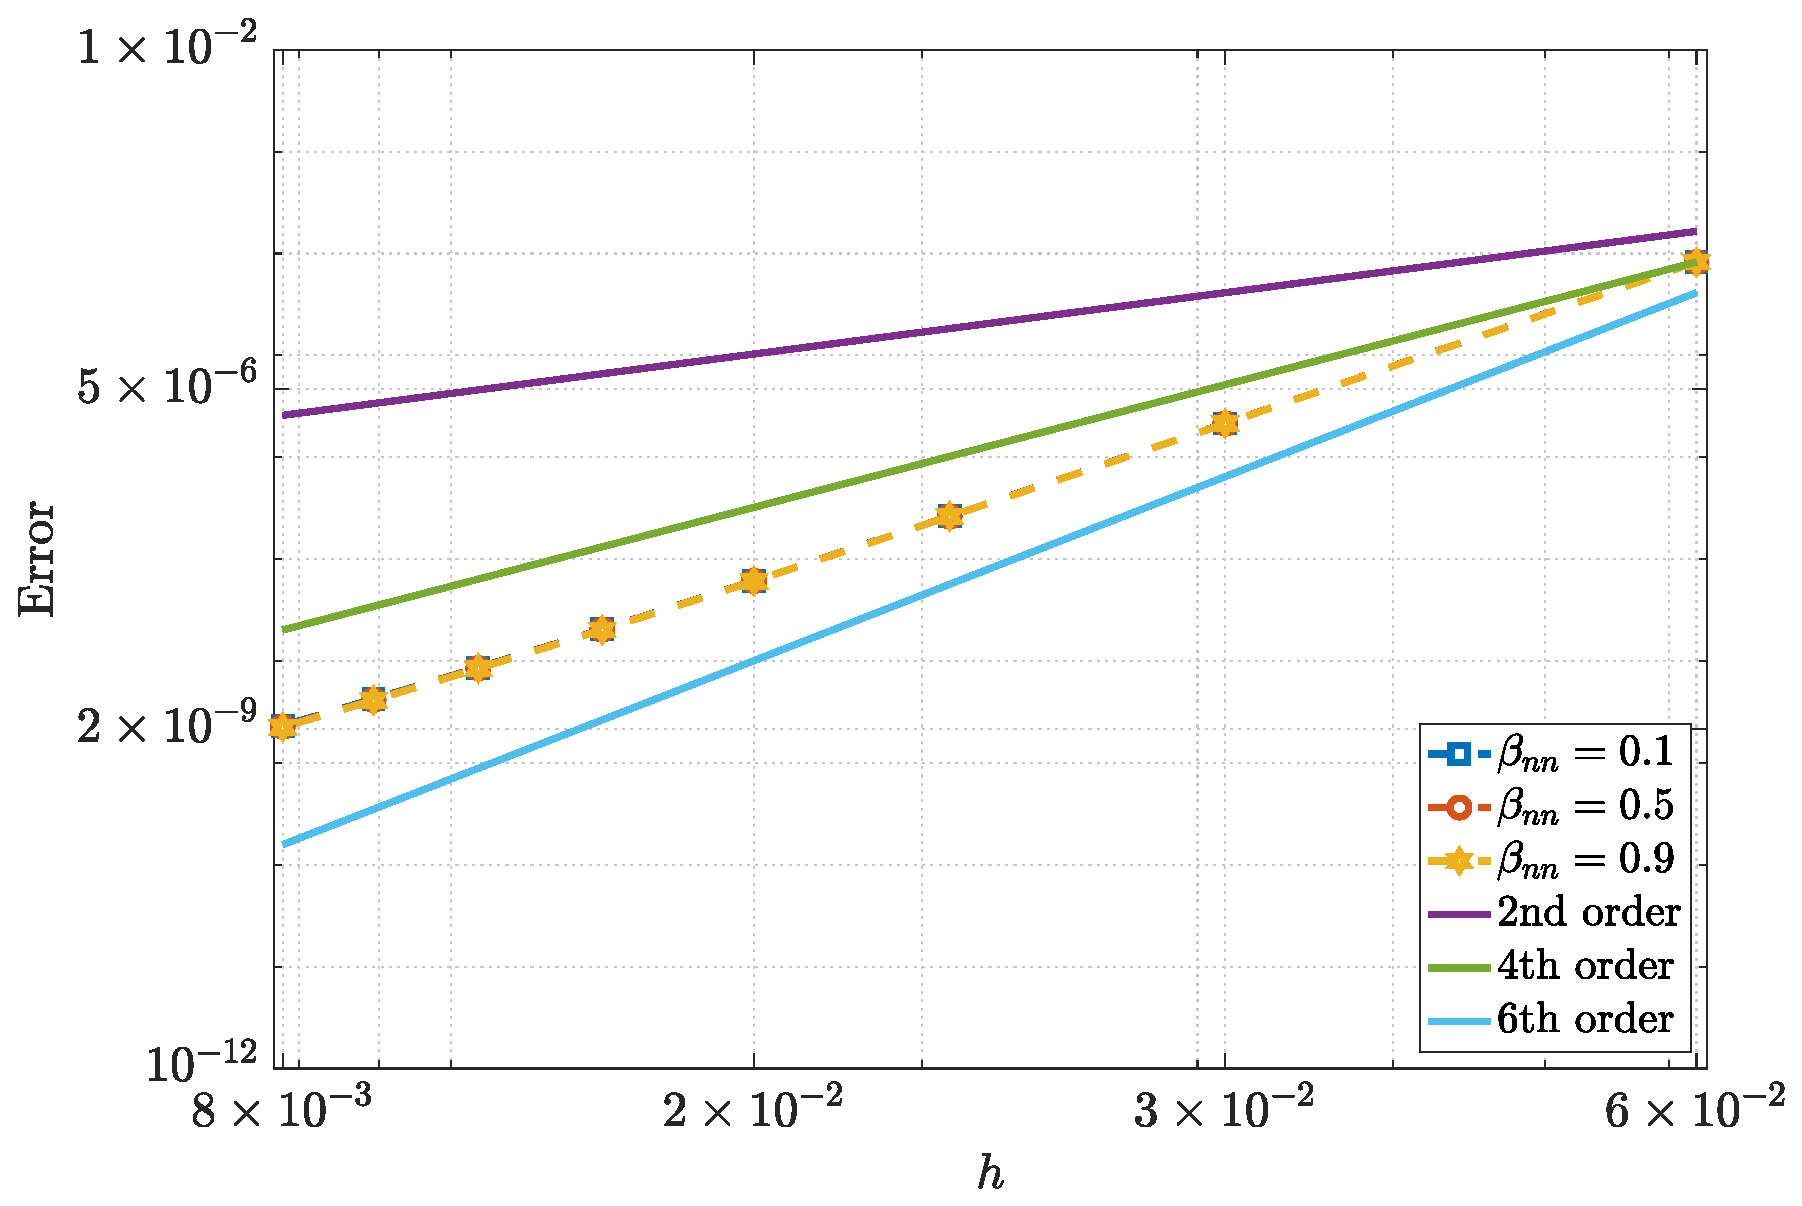
\includegraphics[width=\textwidth]{figures/Case12/Giesekus/Errors/NormErr_2nd_Re_100_Wi_1_epsilon_0_xi_0_alphaG_0.5_Dt_1e-06_at_0.05_tipsim_1_MMS_12_U.eps}
        \caption{$||U - \overline{u}||_{2}$}
        \label{error_u_2nd_Case1_giesekus_alphaG_0.5}
    \end{subfigure}
    \vspace{0.2cm}
    \qquad
    \begin{subfigure}[b]{.47\textwidth}
        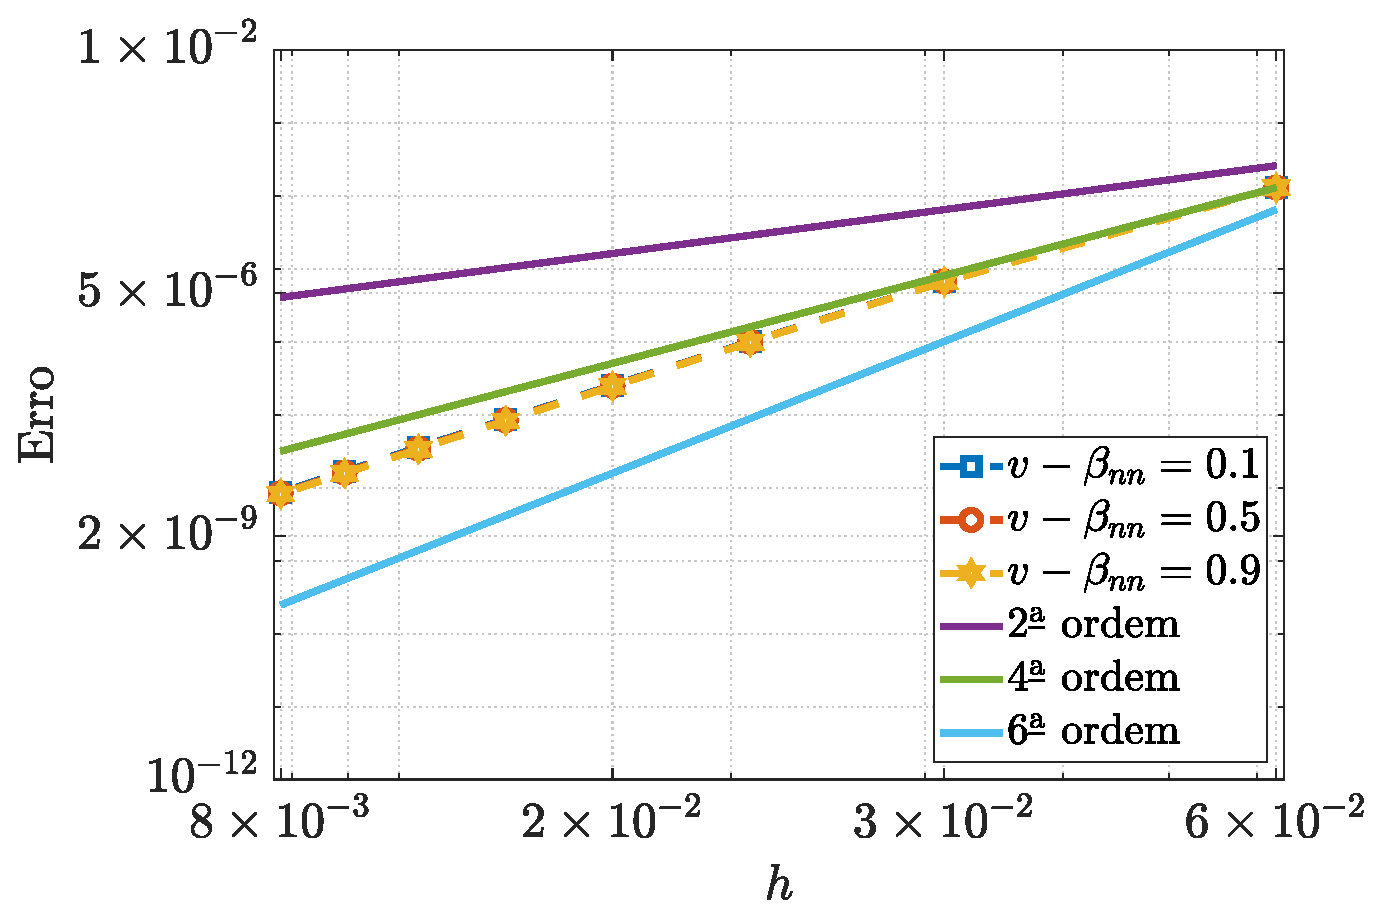
\includegraphics[width=\textwidth]{figures/Case12/Giesekus/Errors/NormErr_2nd_Re_100_Wi_1_epsilon_0_xi_0_alphaG_0.1_Dt_1e-06_at_0.05_tipsim_1_MMS_12_V.eps}
        \caption{$||V - \widetilde{v}||_{2}$}
        \label{error_v_2nd_Case1_giesekus_alphaG_0.5}
    \end{subfigure}
    \qquad
    \begin{subfigure}[b]{.47\textwidth}
        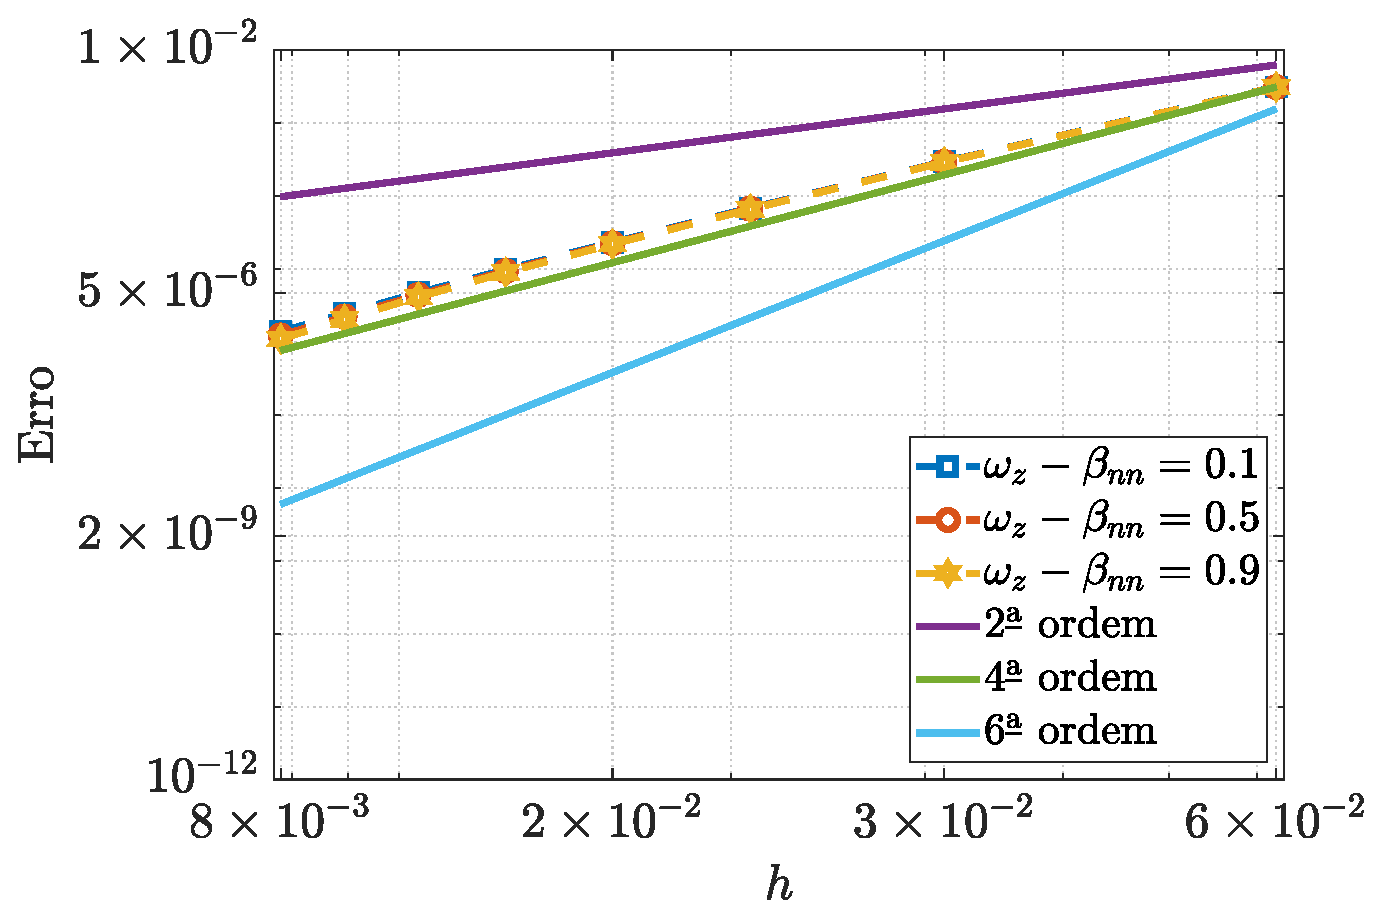
\includegraphics[width=\textwidth]{figures/Case12/Giesekus/Errors/NormErr_2nd_Re_100_Wi_1_epsilon_0_xi_0_alphaG_0.1_Dt_1e-06_at_0.05_tipsim_1_MMS_12_Wz.eps}
        \caption{$||\Omega_{z} - \widetilde{\omega_{z}}||_{2}$}
        \label{error_wz_2nd_Case1_giesekus_alphaG_0.5}
    \end{subfigure}
    \qquad
    \begin{subfigure}[b]{.47\textwidth}
        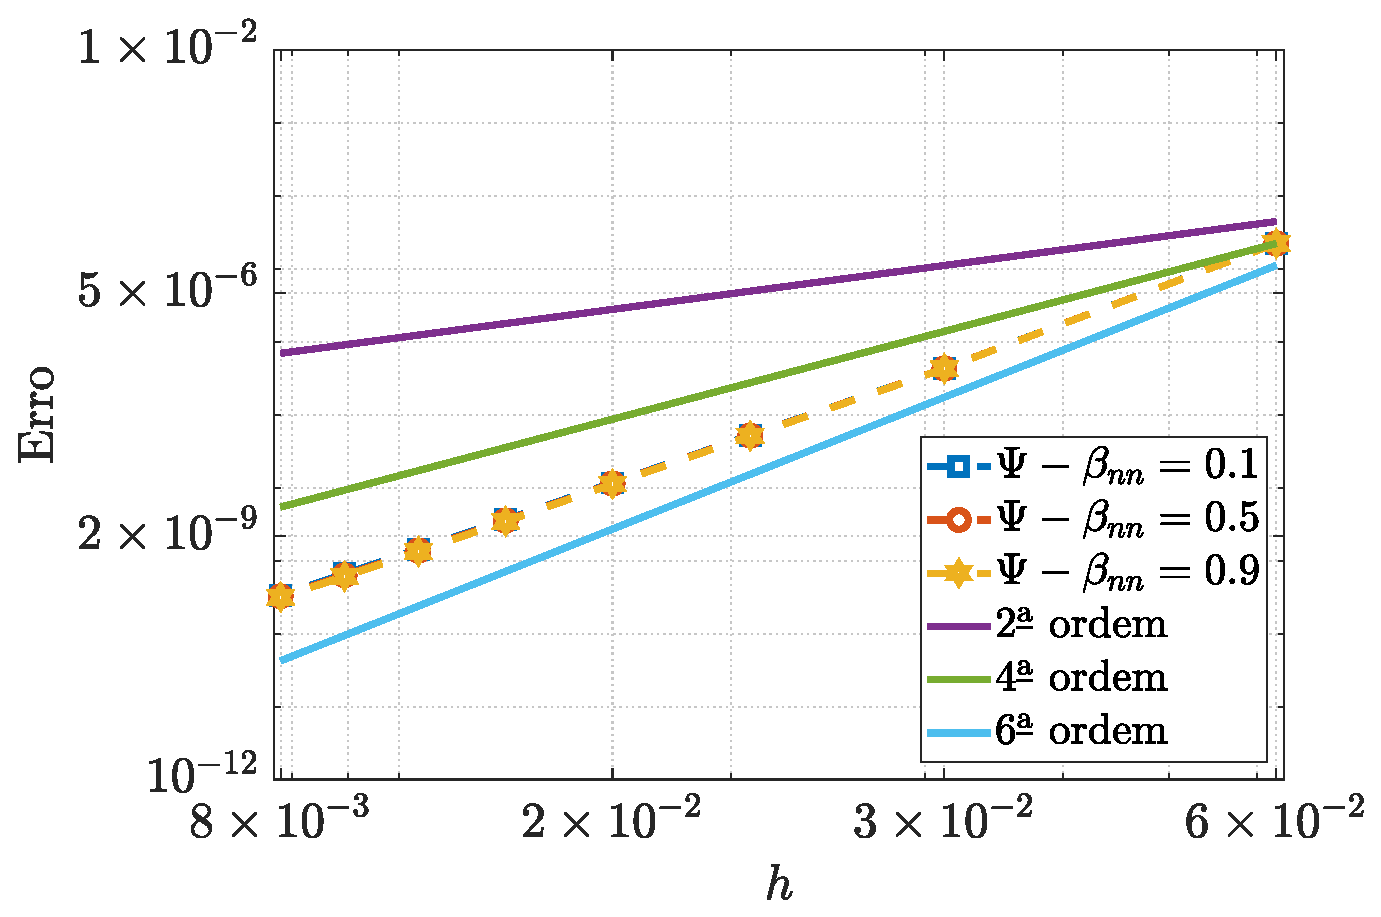
\includegraphics[width=\textwidth]{figures/Case12/Giesekus/Errors/NormErr_2nd_Re_100_Wi_1_epsilon_0_xi_0_alphaG_0.1_Dt_1e-06_at_0.05_tipsim_1_MMS_12_Psi.eps}
        \caption{$||\Psi - \widetilde{\Psi}||_{2}$}
        \label{error_psi_2nd_Case1_oldorydbgiesekus_alphaG_0.5}
    \end{subfigure}
    \fdadospesquisa
\end{figure}

A \autoref{GEerror052} exibe gráficos de erros representando os componentes do tensor extra-tensões, para o escoamento de fluido viscoelástico com o modelo Giesekus com $Re=100$, $Wi=1$ e $\alpha_G=0.5$.
\begin{figure}[H] 
    \centering
    \caption{Erro para os componentes dos tensores extra-tensões, utilizando os parâmetros $Re=100,$ $Wi=1$ e $\alpha_{G} = 0.5$, para o escoamento de fluido viscoelástico Giesekus}\label{GEerror052}
    \begin{subfigure}[b]{.47\textwidth}
        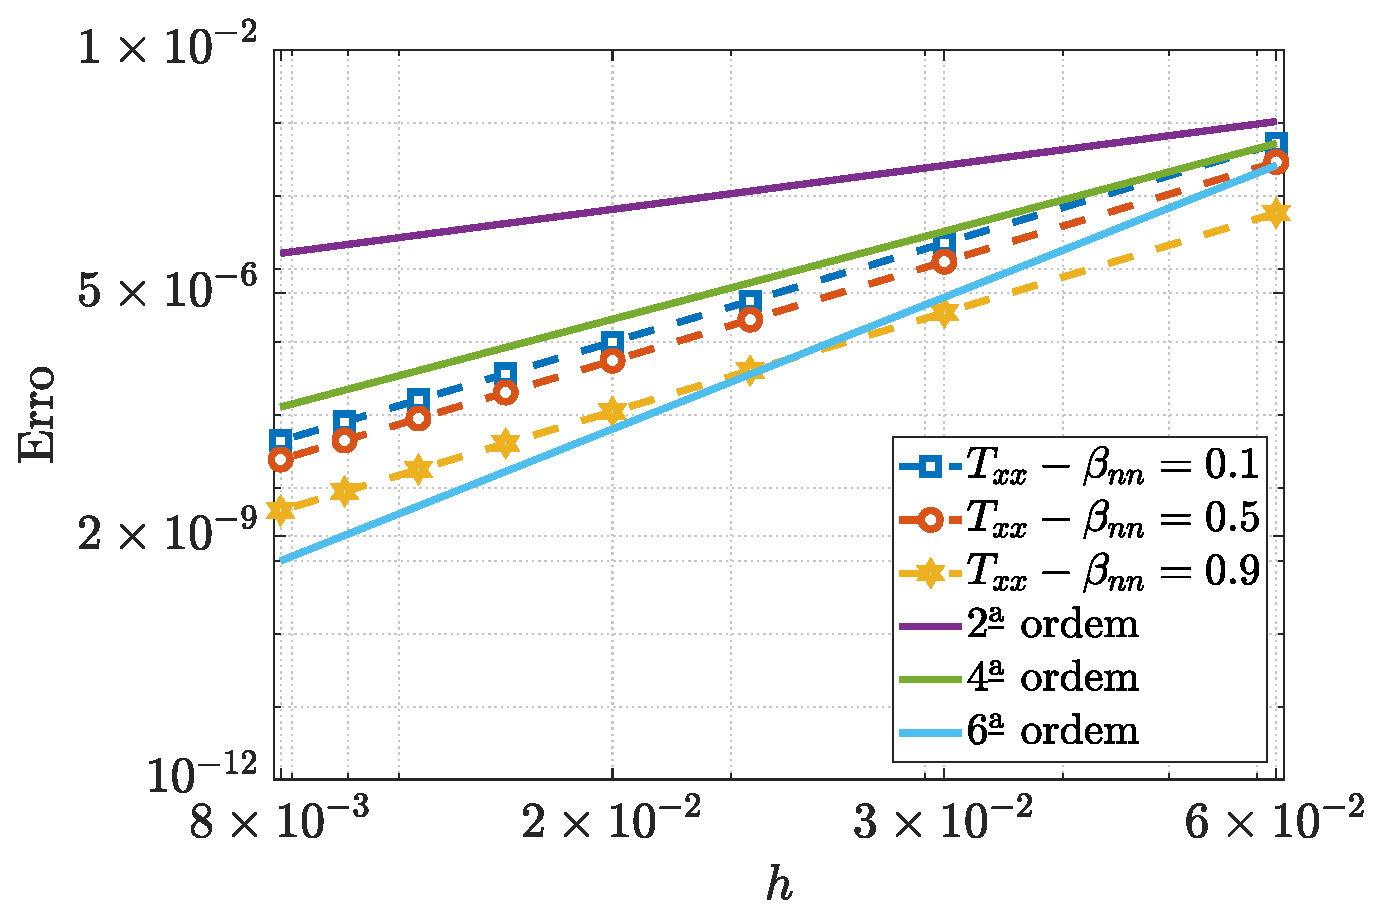
\includegraphics[width=\textwidth]{figures/Case12/Giesekus/Errors/NormErr_2nd_Re_100_Wi_1_epsilon_0_xi_0_alphaG_0.1_Dt_1e-06_at_0.05_tipsim_1_MMS_12_Txx.eps}
        \caption{$||T_{xx} - \overline{T}_{xx}||_{2}$}
        \label{error_txx_2nd_Case1_giesekus_alphaG_0.5}
    \end{subfigure}
    \vspace{0.2cm}
    \qquad
    \begin{subfigure}[b]{.47\textwidth}
        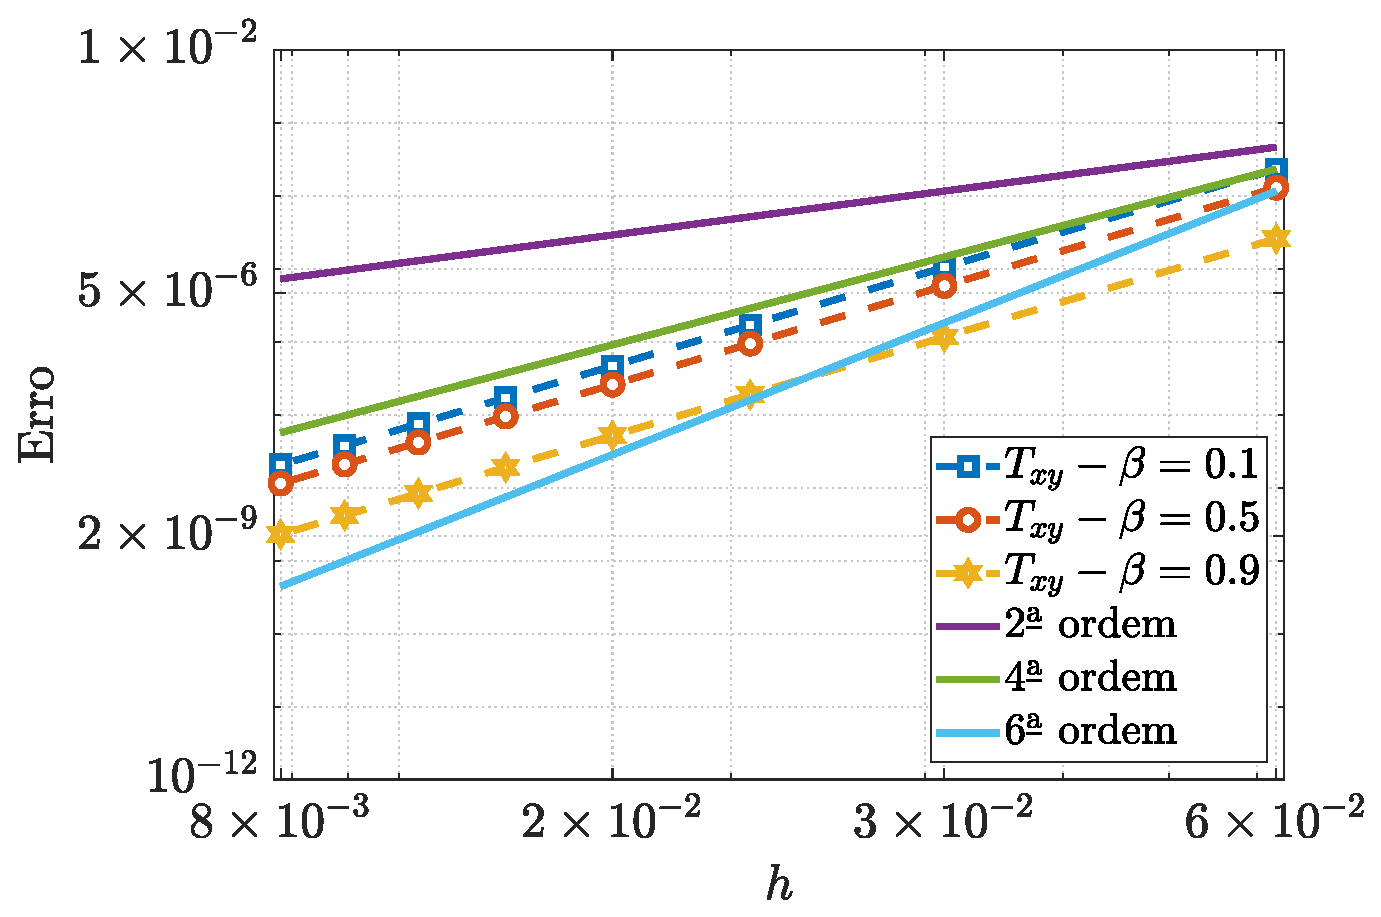
\includegraphics[width=\textwidth]{figures/Case12/Giesekus/Errors/NormErr_2nd_Re_100_Wi_1_epsilon_0_xi_0_alphaG_0.1_Dt_1e-06_at_0.05_tipsim_1_MMS_12_Txy.eps}
        \caption{$||T_{xy} - \overline{T}_{xy}||_{2}$}
        \label{error_txy_2nd_Case1_giesekus_alphaG_0.5}
    \end{subfigure}
    \qquad
    \begin{subfigure}[b]{.47\textwidth}
        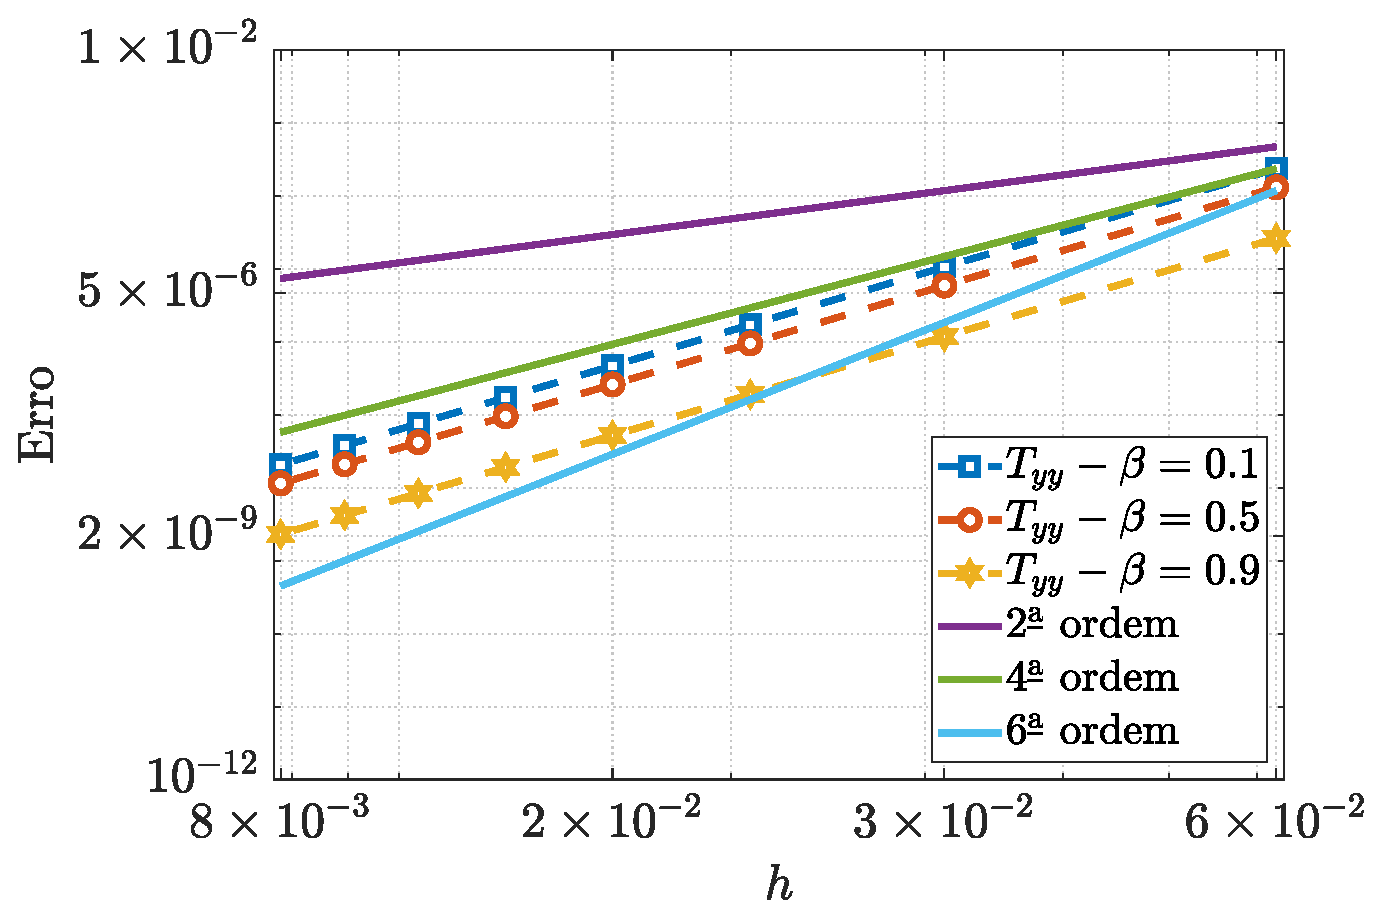
\includegraphics[width=\textwidth]{figures/Case12/Giesekus/Errors/NormErr_2nd_Re_100_Wi_1_epsilon_0_xi_0_alphaG_0.1_Dt_1e-06_at_0.05_tipsim_1_MMS_12_Tyy.eps}
        \caption{$||T_{yy} - \overline{T}_{yy}||_{2}$}
        \label{error_tyy_2nd_Case1_giesekus_alphaG_0.5}
    \end{subfigure}
    \fautor
\end{figure}

Nas simulações com $\alpha_G = 0.5$, apresentadas nas Figuras \ref{GEerror051} e \ref{GEerror052}, observa-se uma similaridade nos resultados em comparação com aqueles obtidos com $\alpha_G = 0.1$. A ordem de convergência permanece consistente, aproximando-se de 4.5 para todas as variáveis estudadas, incluindo os tensores de tensões e a vorticidade. Isso indica que o modelo de Giesekus é estável e preciso em uma ampla gama de valores de $\alpha_G$, tornando-o aplicável em diversas condições de escoamento. Além disso, a precisão do modelo é mantida mesmo com o aumento do parâmetro $\alpha_G$, sugerindo que o esquema numérico implementado é robusto o suficiente para simular diferentes regimes de viscosidade e elasticidade em fluidos viscoelásticos.
\begin{table}[H]
	\IBGEtab{
		\caption{Erros numéricos e cálculo da ordem de convergência para o componente do tensor de tensões $T_{yy}$, utilizando os parâmetros $Wi = 1$ e $\alpha_G = 0.1$, para o escoamento de fluido viscoelástico de Giesekus}\label{tab:GiesekusWzalphaG05Resumida}
	}{
            \begin{tabular*}{\textwidth}{@{\extracolsep\fill}c|c|cc|cc|cc|cc@{}}
                \toprule
                \multirow{2}{*}{$Re$} & \multirow{2}{*}{Malha} & \multicolumn{2}{c}{$\beta_{nn}=0.1$}  & \multicolumn{2}{c}{$\beta_{nn}=0.5$}  & \multicolumn{2}{c}{$\beta_{nn}=0.9$}  & \multicolumn{2}{c}{$\beta_{nn}=1.0$}  \\
                \cline{3-10}
                 & & Erro & p & Erro & p & Erro & p & Erro & p \\
                \midrule
                \multirow{10}{*}{1.00} & 17$\times$17 & 2.34e-04 & --- & 1.30e-04 & --- & 2.60e-05 & --- & 2.60e-18 & --- \\
                & 33$\times$33 & 1.06e-05 & 4.46 & 5.90e-06 & 4.46 & 1.18e-06 & 4.46 & 1.18e-19 & 4.46 \\
                & 49$\times$49 & 1.72e-06 & 4.49 & 9.56e-07 & 4.49 & 1.91e-07 & 4.49 & 1.91e-20 & 4.49 \\
                & 65$\times$65 & 4.72e-07 & 4.49 & 2.62e-07 & 4.49 & 5.25e-08 & 4.49 & 5.25e-21 & 4.49 \\
                & 81$\times$81 & 1.73e-07 & 4.50 & 9.62e-08 & 4.50 & 1.93e-08 & 4.50 & 1.92e-21 & 4.50 \\
                & 97$\times$97 & 7.63e-08 & 4.50 & 4.24e-08 & 4.50 & 8.48e-09 & 4.50 & 8.47e-22 & 4.50 \\
                & 113$\times$113 & 3.81e-08 & 4.50 & 2.12e-08 & 4.50 & 4.24e-09 & 4.50 & 4.24e-22 & 4.50 \\
                & 129$\times$129 & 2.09e-08 & 4.50 & 1.16e-08 & 4.50 & 2.33e-09 & 4.50 & 2.32e-22 & 4.50 \\
                \midrule
                \multirow{10}{*}{100.00} & 17$\times$17 & 2.35e-04 & --- & 1.31e-04 & --- & 2.61e-05 & --- & 2.61e-18 & --- \\
                & 33$\times$33 & 1.06e-05 & 4.48 & 5.86e-06 & 4.48 & 1.17e-06 & 4.48 & 1.17e-19 & 4.48 \\
                & 49$\times$49 & 1.70e-06 & 4.50 & 9.46e-07 & 4.50 & 1.89e-07 & 4.50 & 1.89e-20 & 4.50 \\
                & 65$\times$65 & 4.67e-07 & 4.50 & 2.59e-07 & 4.50 & 5.19e-08 & 4.50 & 5.18e-21 & 4.50 \\
                & 81$\times$81 & 1.71e-07 & 4.50 & 9.50e-08 & 4.50 & 1.90e-08 & 4.50 & 1.90e-21 & 4.50 \\
                & 97$\times$97 & 7.52e-08 & 4.50 & 4.18e-08 & 4.50 & 8.36e-09 & 4.50 & 8.36e-22 & 4.50 \\
                & 113$\times$113 & 3.76e-08 & 4.50 & 2.09e-08 & 4.50 & 4.18e-09 & 4.50 & 4.18e-22 & 4.50 \\
                & 129$\times$129 & 2.06e-08 & 4.50 & 1.15e-08 & 4.50 & 2.29e-09 & 4.50 & 2.29e-22 & 4.50 \\
                \midrule
                \multirow{10}{*}{400.00} & 17$\times$17 & 2.37e-04 & --- & 1.32e-04 & --- & 2.63e-05 & --- & 2.63e-18 & --- \\
                & 33$\times$33 & 1.04e-05 & 4.51 & 5.78e-06 & 4.51 & 1.16e-06 & 4.51 & 1.16e-19 & 4.51 \\
                & 49$\times$49 & 1.66e-06 & 4.52 & 9.24e-07 & 4.52 & 1.85e-07 & 4.52 & 1.85e-20 & 4.52 \\
                & 65$\times$65 & 4.54e-07 & 4.52 & 2.52e-07 & 4.52 & 5.04e-08 & 4.52 & 5.04e-21 & 4.52 \\
                & 81$\times$81 & 1.66e-07 & 4.51 & 9.21e-08 & 4.51 & 1.84e-08 & 4.51 & 1.84e-21 & 4.51 \\
                & 97$\times$97 & 7.28e-08 & 4.51 & 4.04e-08 & 4.51 & 8.09e-09 & 4.51 & 8.08e-22 & 4.51 \\
                & 113$\times$113 & 3.63e-08 & 4.51 & 2.02e-08 & 4.51 & 4.04e-09 & 4.51 & 4.03e-22 & 4.51 \\
                & 129$\times$129 & 1.99e-08 & 4.51 & 1.11e-08 & 4.51 & 2.21e-09 & 4.51 & 2.21e-22 & 4.51 \\
                \midrule
                \multirow{10}{*}{1000.00} & 17$\times$17 & 2.43e-04 & --- & 1.35e-04 & --- & 2.70e-05 & --- & 2.70e-18 & --- \\
                & 33$\times$33 & 1.03e-05 & 4.56 & 5.73e-06 & 4.56 & 1.15e-06 & 4.56 & 1.14e-19 & 4.56 \\
                & 49$\times$49 & 1.62e-06 & 4.56 & 9.02e-07 & 4.56 & 1.80e-07 & 4.56 & 1.80e-20 & 4.56 \\
                & 65$\times$65 & 4.39e-07 & 4.54 & 2.44e-07 & 4.54 & 4.88e-08 & 4.54 & 4.88e-21 & 4.54 \\
                & 81$\times$81 & 1.60e-07 & 4.53 & 8.88e-08 & 4.53 & 1.78e-08 & 4.53 & 1.77e-21 & 4.53 \\
                & 97$\times$97 & 7.00e-08 & 4.53 & 3.89e-08 & 4.53 & 7.78e-09 & 4.53 & 7.77e-22 & 4.53 \\
                & 113$\times$113 & 3.48e-08 & 4.52 & 1.94e-08 & 4.52 & 3.87e-09 & 4.52 & 3.87e-22 & 4.52 \\
                & 129$\times$129 & 1.91e-08 & 4.52 & 1.06e-08 & 4.52 & 2.12e-09 & 4.52 & 2.12e-22 & 4.52 \\
                \bottomrule
            \end{tabular*}
	}{%
	\fdadospesquisa
	}
\end{table}

\begin{table}[H]
	\IBGEtab{
	   \caption{Erros numéricos e cálculo da ordem de convergência para o componente do tensor de tensões $T_{yy}$, utilizando os parâmetros $Wi = 1$ e $\alpha_G = 0.5$, para o escoamento de fluido viscoelástico de Giesekus}\label{tab:GiesekusTyyalphaG05Resumida}
	}{
            \begin{tabular*}{\textwidth}{@{\extracolsep\fill}c|c|cc|cc|cc|cc@{}}
                \toprule
                \multirow{2}{*}{$Re$} & \multirow{2}{*}{Malha} & \multicolumn{2}{c}{$\beta_{nn}=0.1$}  & \multicolumn{2}{c}{$\beta_{nn}=0.5$}  & \multicolumn{2}{c}{$\beta_{nn}=0.9$}  & \multicolumn{2}{c}{$\beta_{nn}=1.0$}  \\
                \cline{3-10}
                 & & Erro & p & Erro & p & Erro & p & Erro & p \\
                \midrule
                \multirow{10}{*}{1.00} & 17$\times$17 & 2.34e-04 & --- & 1.30e-04 & --- & 2.60e-05 & --- & 2.60e-18 & --- \\
                & 33$\times$33 & 1.06e-05 & 4.46 & 5.90e-06 & 4.46 & 1.18e-06 & 4.46 & 1.18e-19 & 4.46 \\
                & 49$\times$49 & 1.72e-06 & 4.49 & 9.56e-07 & 4.49 & 1.91e-07 & 4.49 & 1.91e-20 & 4.49 \\
                & 65$\times$65 & 4.72e-07 & 4.49 & 2.62e-07 & 4.49 & 5.25e-08 & 4.49 & 5.24e-21 & 4.49 \\
                & 81$\times$81 & 1.73e-07 & 4.50 & 9.62e-08 & 4.50 & 1.92e-08 & 4.50 & 1.92e-21 & 4.50 \\
                & 97$\times$97 & 7.62e-08 & 4.50 & 4.24e-08 & 4.50 & 8.48e-09 & 4.50 & 8.47e-22 & 4.50 \\
                & 113$\times$113 & 3.81e-08 & 4.50 & 2.12e-08 & 4.50 & 4.24e-09 & 4.50 & 4.23e-22 & 4.50 \\
                & 129$\times$129 & 2.09e-08 & 4.50 & 1.16e-08 & 4.50 & 2.32e-09 & 4.50 & 2.32e-22 & 4.50 \\
                \midrule
                \multirow{10}{*}{100.00} & 17$\times$17 & 2.38e-04 & --- & 1.32e-04 & --- & 2.64e-05 & --- & 2.64e-18 & --- \\
                & 33$\times$33 & 1.04e-05 & 4.52 & 5.76e-06 & 4.52 & 1.15e-06 & 4.52 & 1.15e-19 & 4.52 \\
                & 49$\times$49 & 1.65e-06 & 4.53 & 9.19e-07 & 4.53 & 1.84e-07 & 4.53 & 1.84e-20 & 4.53 \\
                & 65$\times$65 & 4.50e-07 & 4.52 & 2.50e-07 & 4.52 & 5.00e-08 & 4.52 & 5.00e-21 & 4.52 \\
                & 81$\times$81 & 1.64e-07 & 4.52 & 9.13e-08 & 4.52 & 1.83e-08 & 4.52 & 1.83e-21 & 4.52 \\
                & 97$\times$97 & 7.22e-08 & 4.51 & 4.01e-08 & 4.51 & 8.02e-09 & 4.51 & 8.01e-22 & 4.51 \\
                & 113$\times$113 & 3.60e-08 & 4.51 & 2.00e-08 & 4.51 & 4.00e-09 & 4.51 & 4.00e-22 & 4.51 \\
                & 129$\times$129 & 1.97e-08 & 4.51 & 1.10e-08 & 4.51 & 2.19e-09 & 4.51 & 2.19e-22 & 4.51 \\
                \midrule
                \multirow{10}{*}{400.00} & 17$\times$17 & 2.56e-04 & --- & 1.42e-04 & --- & 2.84e-05 & --- & 2.84e-18 & --- \\
                & 33$\times$33 & 1.04e-05 & 4.61 & 5.80e-06 & 4.61 & 1.16e-06 & 4.61 & 1.16e-19 & 4.61 \\
                & 49$\times$49 & 1.61e-06 & 4.60 & 8.97e-07 & 4.60 & 1.79e-07 & 4.60 & 1.79e-20 & 4.60 \\
                & 65$\times$65 & 4.33e-07 & 4.58 & 2.40e-07 & 4.58 & 4.81e-08 & 4.58 & 4.80e-21 & 4.58 \\
                & 81$\times$81 & 1.56e-07 & 4.56 & 8.69e-08 & 4.56 & 1.74e-08 & 4.56 & 1.74e-21 & 4.56 \\
                & 97$\times$97 & 6.83e-08 & 4.55 & 3.79e-08 & 4.55 & 7.58e-09 & 4.55 & 7.58e-22 & 4.55 \\
                & 113$\times$113 & 3.39e-08 & 4.54 & 1.88e-08 & 4.54 & 3.77e-09 & 4.54 & 3.76e-22 & 4.54 \\
                & 129$\times$129 & 1.85e-08 & 4.54 & 1.03e-08 & 4.53 & 2.06e-09 & 4.53 & 2.05e-22 & 4.53 \\
                \midrule
                \multirow{10}{*}{1000.00} & 17$\times$17 & 3.11e-04 & --- & 1.73e-04 & --- & 3.46e-05 & --- & 3.46e-18 & --- \\
                & 33$\times$33 & 1.17e-05 & 4.74 & 6.47e-06 & 4.74 & 1.29e-06 & 4.74 & 1.29e-19 & 4.74 \\
                & 49$\times$49 & 1.72e-06 & 4.72 & 9.56e-07 & 4.72 & 1.91e-07 & 4.72 & 1.91e-20 & 4.72 \\
                & 65$\times$65 & 4.50e-07 & 4.66 & 2.50e-07 & 4.66 & 5.00e-08 & 4.66 & 5.00e-21 & 4.66 \\
                & 81$\times$81 & 1.60e-07 & 4.62 & 8.91e-08 & 4.62 & 1.78e-08 & 4.62 & 1.78e-21 & 4.62 \\
                & 97$\times$97 & 6.93e-08 & 4.60 & 3.85e-08 & 4.60 & 7.71e-09 & 4.60 & 7.70e-22 & 4.60 \\
                & 113$\times$113 & 3.42e-08 & 4.58 & 1.90e-08 & 4.58 & 3.80e-09 & 4.58 & 3.80e-22 & 4.58 \\
                & 129$\times$129 & 1.86e-08 & 4.57 & 1.03e-08 & 4.57 & 2.06e-09 & 4.57 & 2.06e-22 & 4.57 \\
                \bottomrule
            \end{tabular*}
	}{
		\fdadospesquisa
	}
\end{table}

\subsection{Caso de verificação usando o modelo LPTT}

As simulações numéricas realizadas para verificar o código de alta ordem desenvolvido para escoamentos de fluidos viscoelásticos foram configuradas utilizando o modelo LPTT (Linear Phan-Thien-Tanner), com números de Reynolds variando entre $Re = 1,\ 100,\ 400$ e $1000$, número de Weissenberg $Wi = 1,\ 5$ e $10$. Além disso, a razão de viscosidade do solvente foi definida como $\beta_{nn} = 0.1,\ 0.5,\ 0.9$ e $1.0$, e os parâmetros adicionais de elasticidade e afinamento por cisalhamento ($\epsilon$ e $\xi$) variaram entre $0.5$ e $1.0$ para $\epsilon$, e $0.1$ e $0.5$ para $\xi$, com o objetivo de avaliar o desempenho do modelo em diferentes regimes de escoamento viscoelástico.

A \autoref{LPTTerror1} apresenta os gráficos de erro para os componentes do campo de velocidade, vorticidade e função de corrente, enquanto a \autoref{LPTTerror2} complementa essa análise mostrando os erros associados aos tensores de tensão extra no escoamento de fluido viscoelástico LPTT. Esses gráficos mostram a evolução dos erros para $Re = 100$, $Wi = 1$, e $\beta_{nn} = 0.1,\ 0.5$ e  $0.9$. Vale destacar que os resultados para $\beta_{nn} = 1$ foram omitidos, pois os erros correspondentes estavam na ordem de $10^{-18}$, o que teria distorcido a visualização comparativa dos outros valores de $\beta_{nn}$.
\begin{figure}[H] 
    \centering 
    \caption{Erro para o campo de velocidade $(\overline{u},\tilde{v})$, vorticidade $(\tilde{\omega_{z}})$, e função de corrente $(\tilde{\psi})$, considerando $Re=100$, $Wi=1$, $\epsilon = 0.5$ e $\xi = 0.1$, para o escoamento de fluido viscoelástico com o modelo LPTT}\label{LPTTerror1}
     \begin{subfigure}[b]{.47\textwidth}
        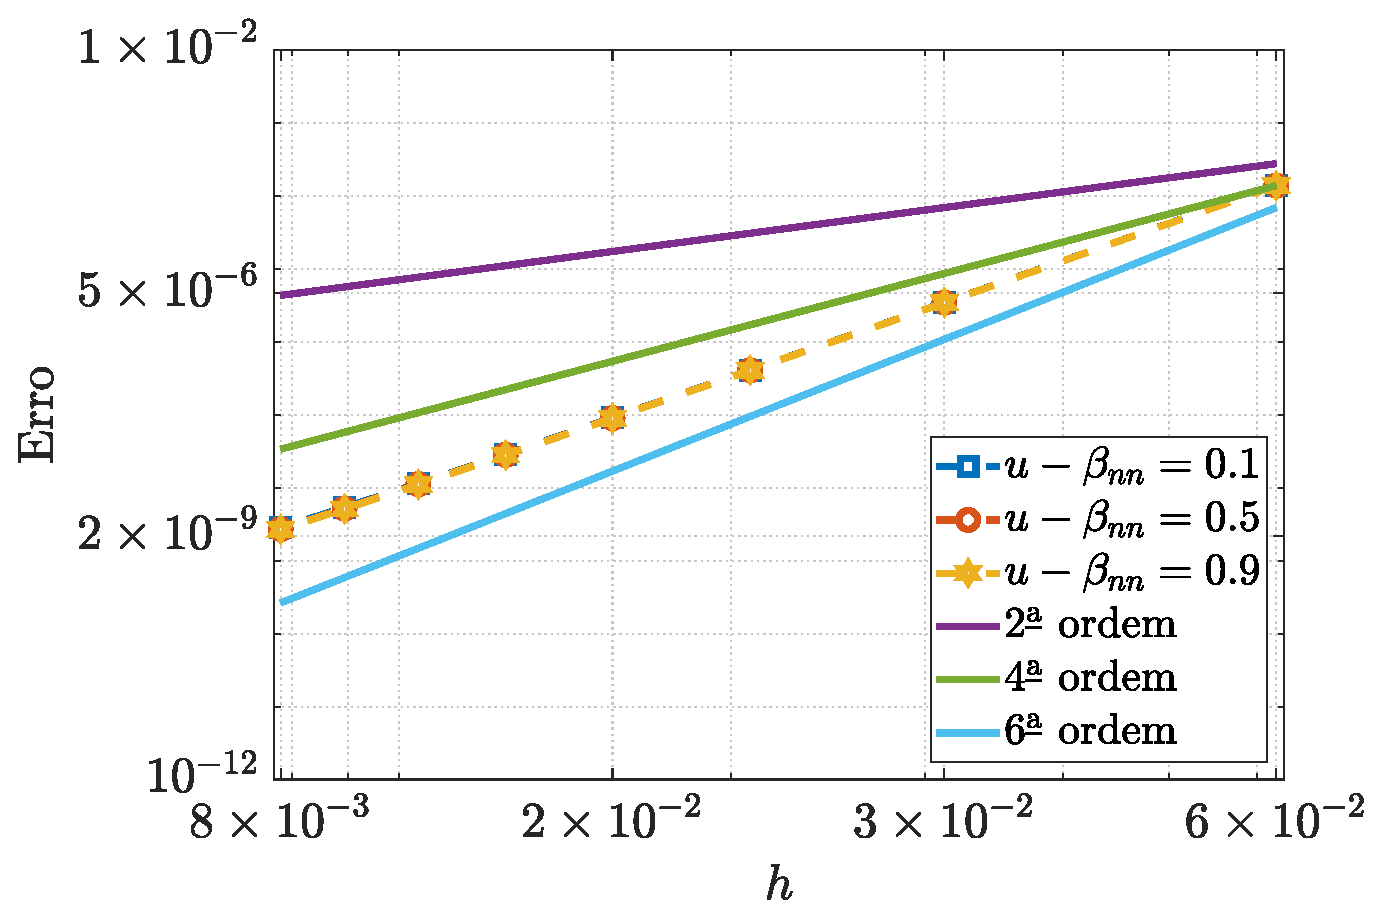
\includegraphics[width=\textwidth]{figures/Case12/LPTT/Errors/NormErr_2nd_Re_100_Wi_1_epsilon_0.5_xi_0.1_alphaG_0_Dt_1e-06_at_0.05_tipsim_1_MMS_12_U.eps}
        \caption{$||U - \overline{u}||_{2}$}
        \label{error_u_2nd_Case1_LPTT_eps_05}
    \end{subfigure}
    \vspace{0.2cm}
    \qquad
    \begin{subfigure}[b]{.47\textwidth}
        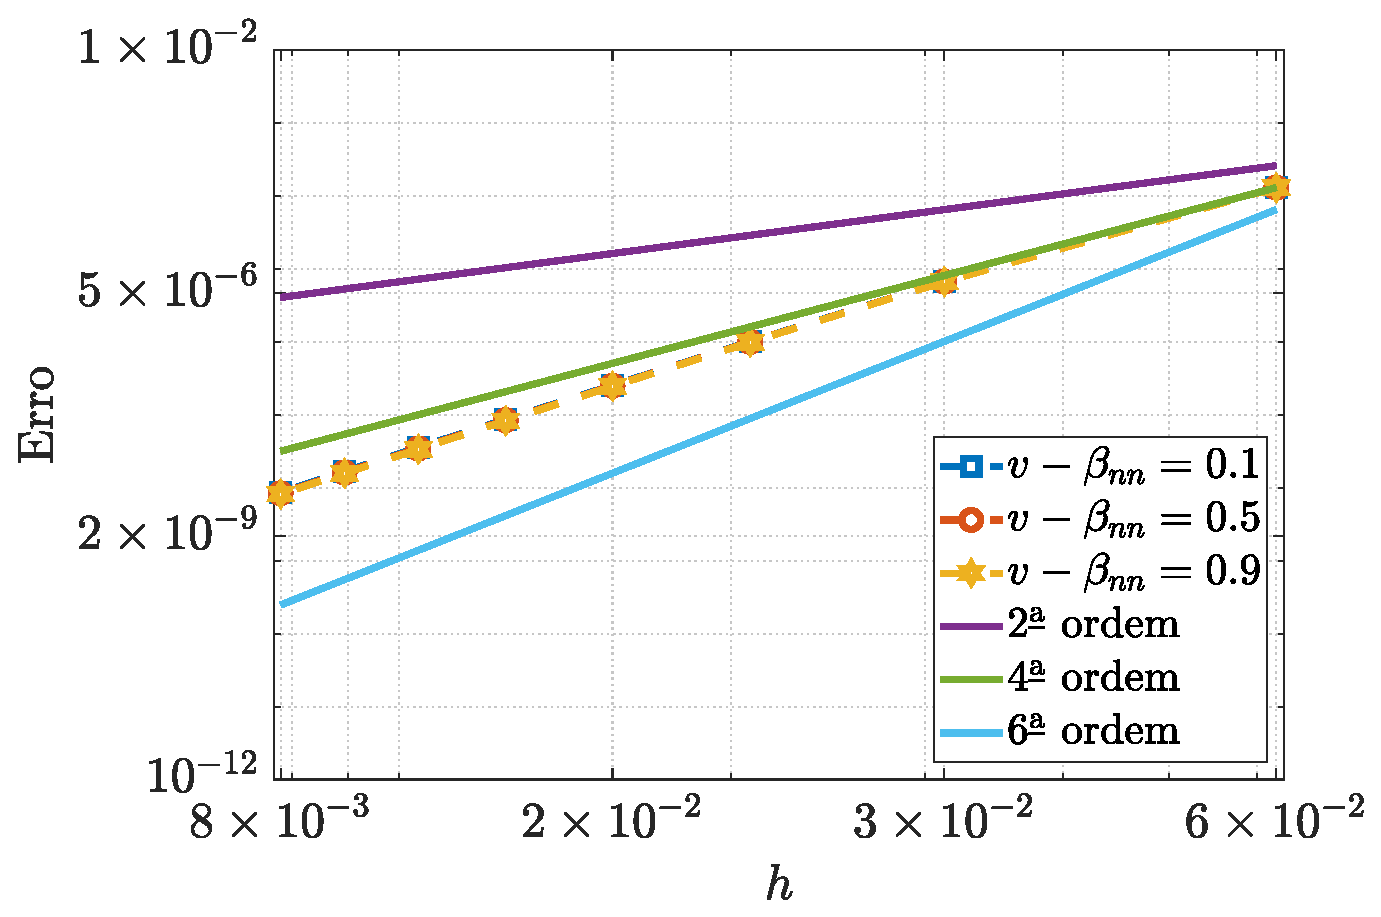
\includegraphics[width=\textwidth]{figures/Case12/LPTT/Errors/NormErr_2nd_Re_100_Wi_1_epsilon_0.5_xi_0.1_alphaG_0_Dt_1e-06_at_0.05_tipsim_1_MMS_12_V.eps}
        \caption{$||V - \widetilde{v}||_{2}$}
        \label{error_v_2nd_Case1_LPTT_eps_05}
    \end{subfigure}
    \qquad
    \begin{subfigure}[b]{.47\textwidth}
        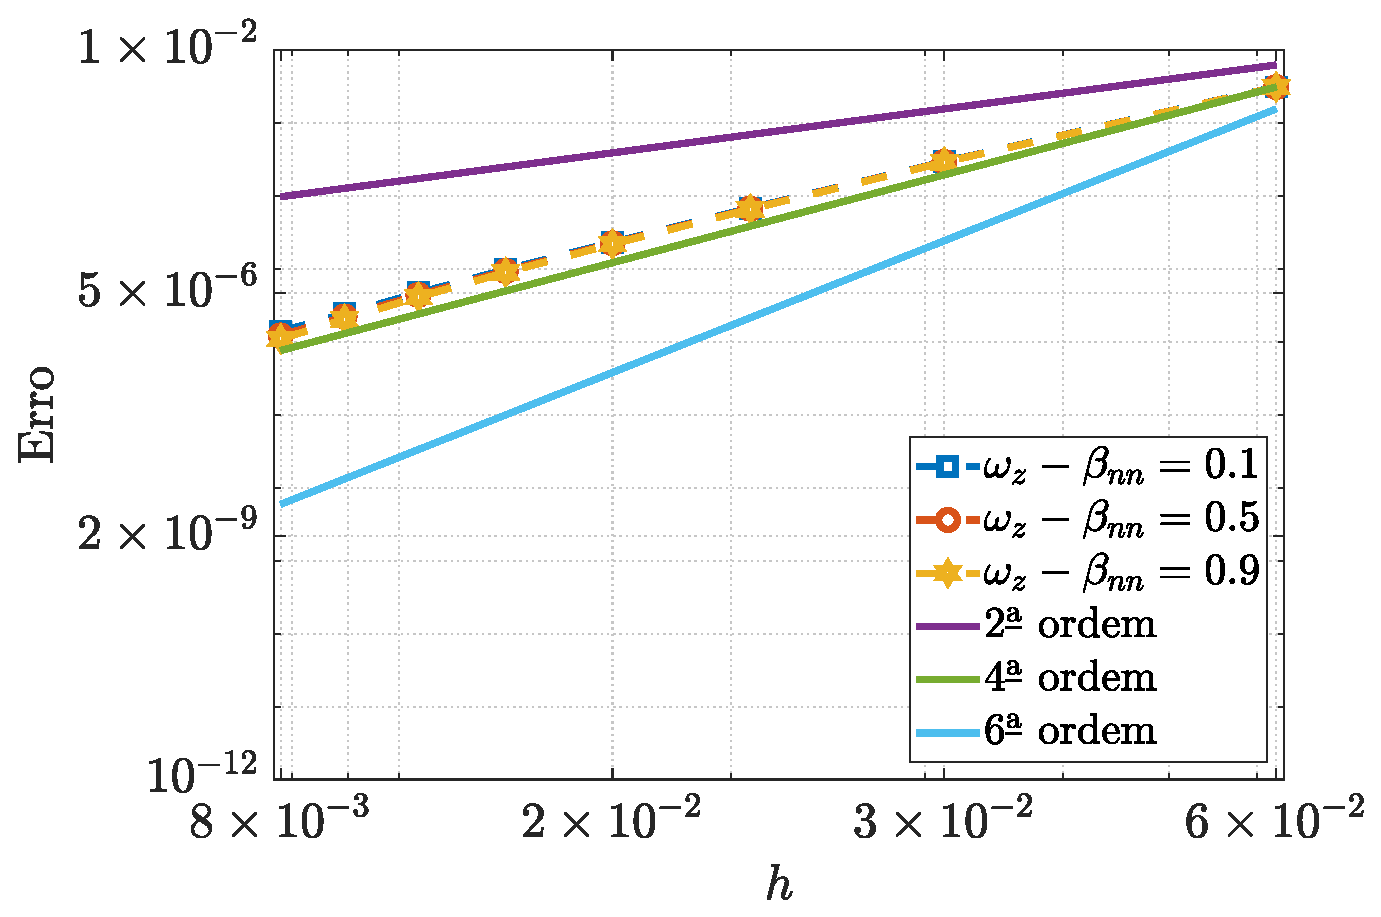
\includegraphics[width=\textwidth]{figures/Case12/LPTT/Errors/NormErr_2nd_Re_100_Wi_1_epsilon_0.5_xi_0.1_alphaG_0_Dt_1e-06_at_0.05_tipsim_1_MMS_12_Wz.eps}
        \caption{$||\Omega_{z} - \widetilde{\omega_{z}}||_{2}$}
        \label{error_wz_2nd_Case1_LPTT_eps_05}
    \end{subfigure}
    \qquad
    \begin{subfigure}[b]{.47\textwidth}
        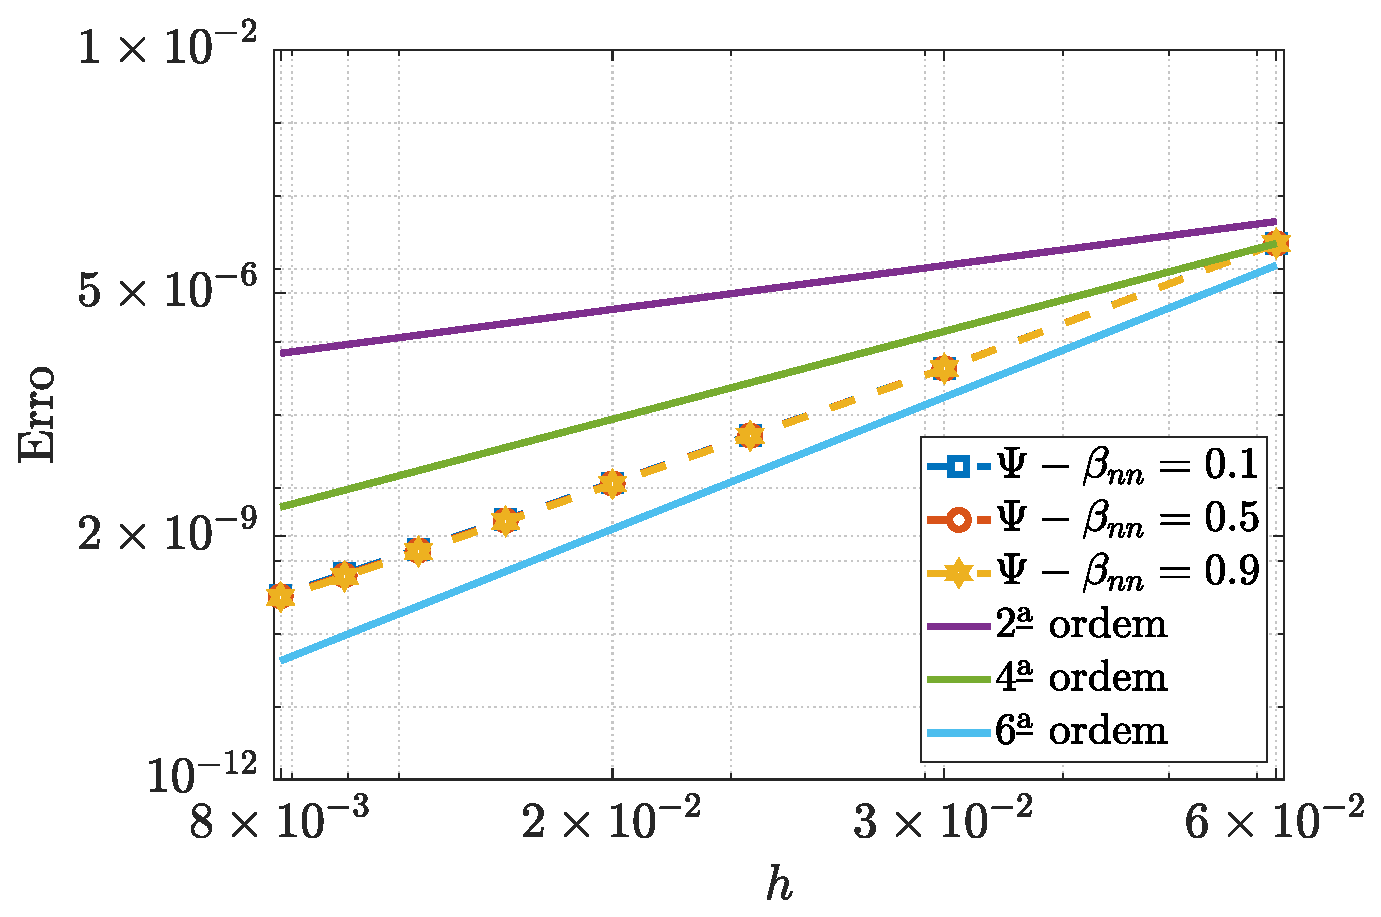
\includegraphics[width=\textwidth]{figures/Case12/LPTT/Errors/NormErr_2nd_Re_100_Wi_1_epsilon_0.5_xi_0.1_alphaG_0_Dt_1e-06_at_0.05_tipsim_1_MMS_12_Psi.eps}
        \caption{$||\Psi - \widetilde{\Psi}||_{2}$}
        \label{error_psi_2nd_Case1_LPTT_eps_05}
    \end{subfigure}
    \fdadospesquisa
\end{figure}

A \autoref{LPTTerror2} exibe gráficos de erros representando os componentes do tensor extra-tensões, para o escoamento de fluido viscoelástico com o modelo LPTT com $Re=100$, $Wi=1$, $\epsilon = 0.5$ e $\xi = 0.1$.
\begin{figure}[H] 
    \centering
    \caption{Erro para os componentes dos tensores extra-tensões, utilizando os parâmetros $Re=100$, $Wi=1$, $\epsilon=0.5$ e $\xi=0.1$, para o escoamento de fluido viscoelástico LPTT}\label{LPTTerror2}
    \begin{subfigure}[b]{.47\textwidth}
        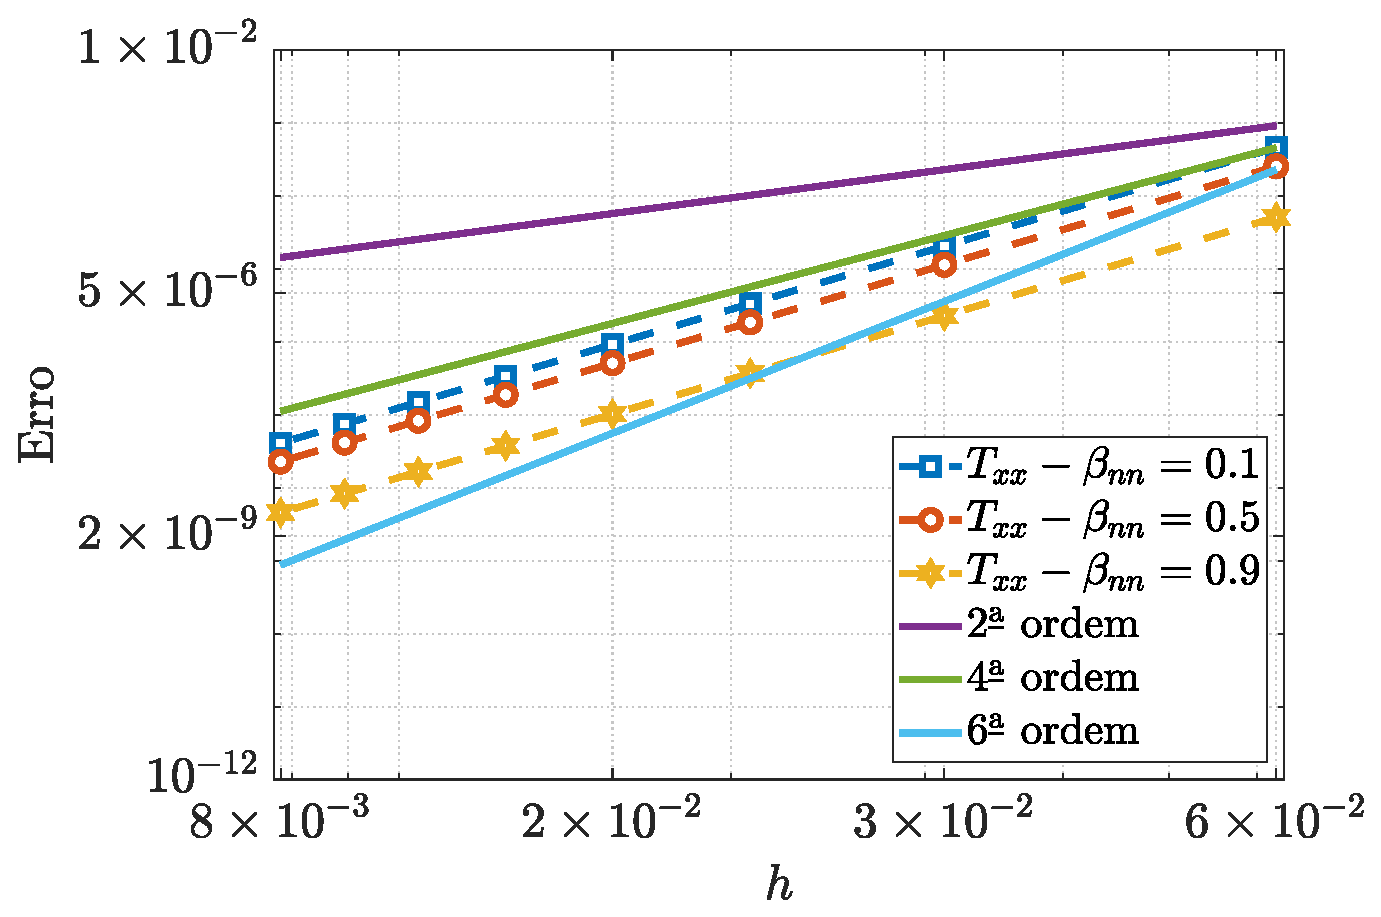
\includegraphics[width=\textwidth]{figures/Case12/LPTT/Errors/NormErr_2nd_Re_100_Wi_1_epsilon_0.5_xi_0.1_alphaG_0_Dt_1e-06_at_0.05_tipsim_1_MMS_12_Txx.eps}
        \caption{$||T_{xx} - \overline{T}_{xx}||_{2}$}
        \label{error_txx_2nd_Case1_LPTT_eps_05}
    \end{subfigure}
    \vspace{0.2cm}
    \qquad
    \begin{subfigure}[b]{.47\textwidth}
        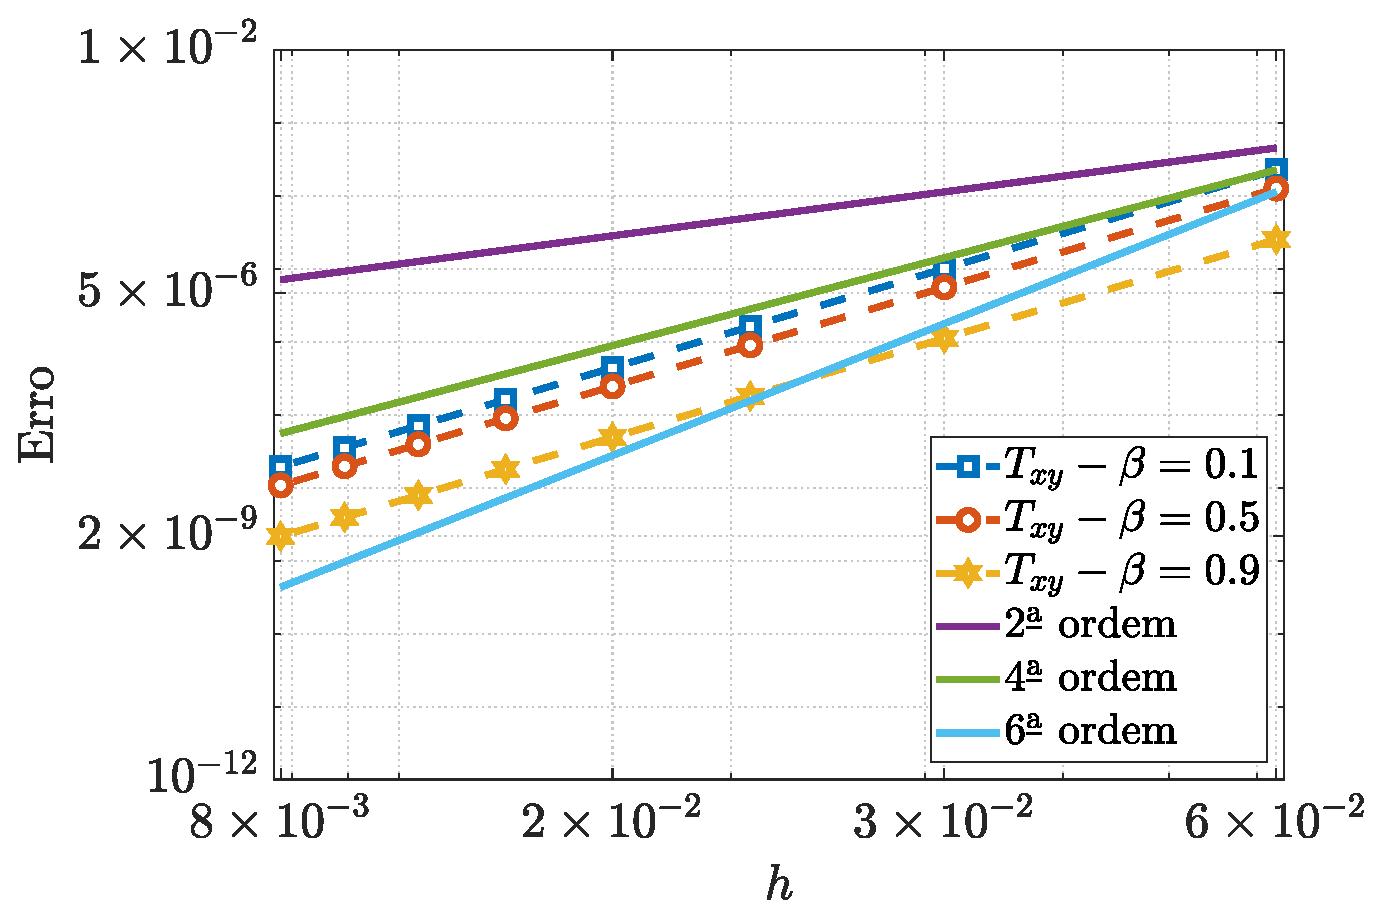
\includegraphics[width=\textwidth]{figures/Case12/LPTT/Errors/NormErr_2nd_Re_100_Wi_1_epsilon_0.5_xi_0.1_alphaG_0_Dt_1e-06_at_0.05_tipsim_1_MMS_12_Txy.eps}
        \caption{$||T_{xy} - \overline{T}_{xy}||_{2}$}
        \label{error_txy_2nd_Case1_LPTT_eps_05}
    \end{subfigure}
    \qquad
    \begin{subfigure}[b]{.47\textwidth}
        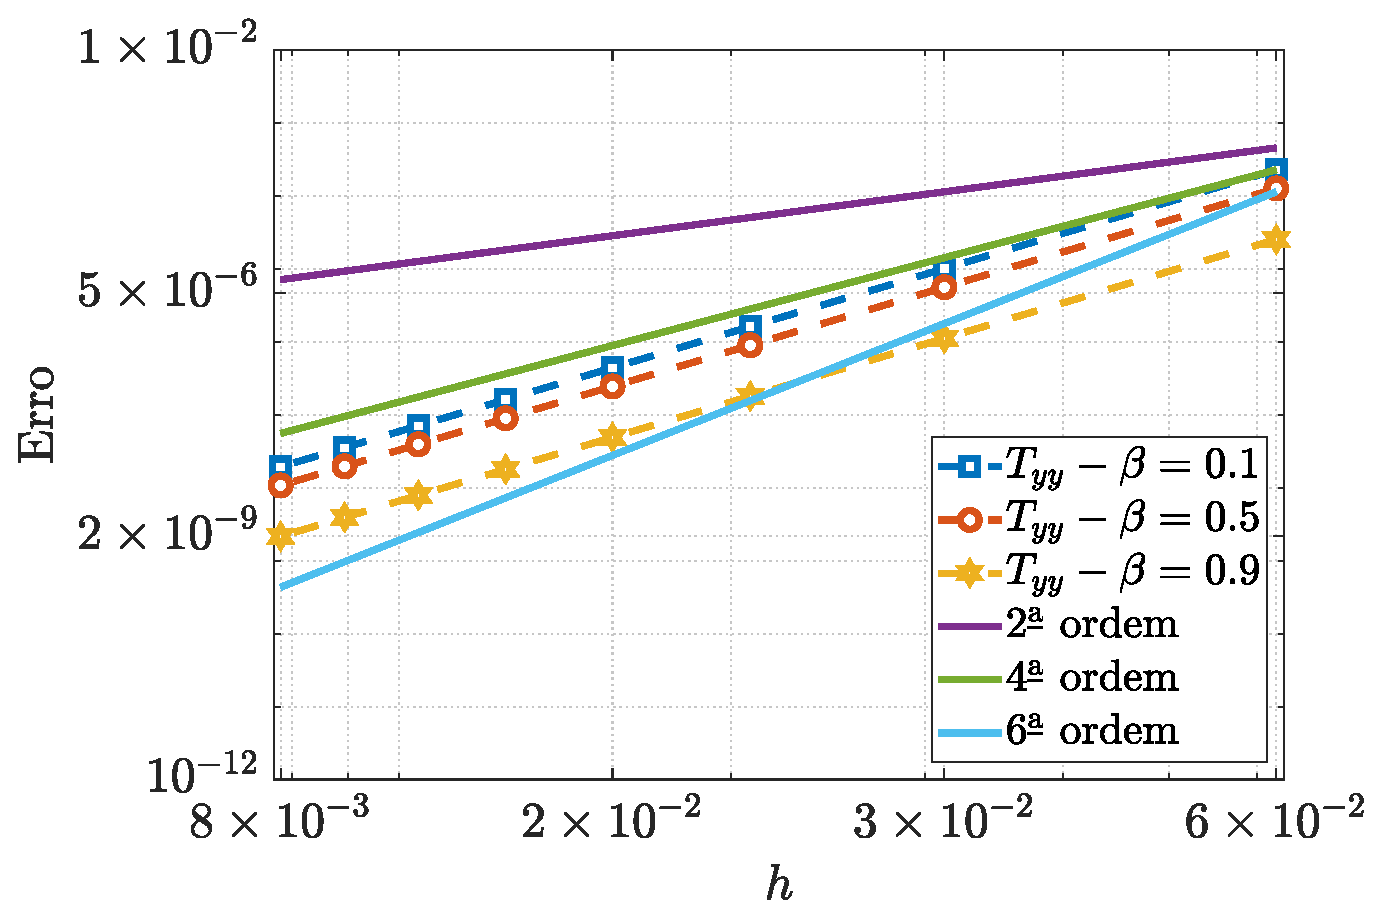
\includegraphics[width=\textwidth]{figures/Case12/LPTT/Errors/NormErr_2nd_Re_100_Wi_1_epsilon_0.5_xi_0.1_alphaG_0_Dt_1e-06_at_0.05_tipsim_1_MMS_12_Tyy.eps}
        \caption{$||T_{yy} - \overline{T}_{yy}||_{2}$}
        \label{error_tyy_2nd_Case1_LPTT_eps_05}
    \end{subfigure}
    \fautor
\end{figure}

A Tabela~\ref{tab_LPTTWzResumida} apresenta os resultados obtidos para a vorticidade $\omega_z$ no contexto do modelo viscoelástico LPTT, considerando os parâmetros fixos $Wi = 1$, $\epsilon = 0.5$ e $\xi = 0.1$. Foram analisadas diversas razões de viscosidade do solvente ($\beta_{nn}$) sob diferentes números de Reynolds ($Re$). A análise numérica avalia os erros absolutos e as ordens de convergência associadas ao refinamento da malha, permitindo verificar a consistência da discretização e a acurácia do esquema adotado para esta variável.

\begin{table}[H]
	\IBGEtab{
		\caption{Erros numéricos e cálculo da ordem de convergência para $\omega_{z}$, usando os parâmetros $Wi=1$, $\epsilon = 0.5$ e $\xi = 0.1$, para o fluxo de fluido viscoelástico de LPTT}\label{tab_LPTTWzResumida}
	}{
		\begin{tabular*}{\textwidth}{@{\extracolsep\fill}c|c|cc|cc|cc|cc@{}}
                \toprule
                \multirow{2}{*}{$Re$} & \multirow{2}{*}{Malha} & \multicolumn{2}{c}{$\beta_{nn}=0.1$}  & \multicolumn{2}{c}{$\beta_{nn}=0.5$}  & \multicolumn{2}{c}{$\beta_{nn}=0.9$}  & \multicolumn{2}{c}{$\beta_{nn}=1.0$}  \\
                \cline{3-10}
                 & & Erro & p & Erro & p & Erro & p & Erro & p \\
                \midrule
                \multirow{10}{*}{1.00} & 17$\times$17 & 3.02e-03 & --- & 2.77e-03 & --- & 2.57e-03 & --- & 2.52e-03 & --- \\
                & 33$\times$33 & 2.54e-04 & 3.57 & 1.70e-04 & 4.03 & 1.35e-04 & 4.25 & 1.29e-04 & 4.29 \\
                & 49$\times$49 & 4.87e-05 & 4.07 & 2.59e-05 & 4.64 & 1.99e-05 & 4.72 & 1.90e-05 & 4.73 \\
                & 65$\times$65 & 1.32e-05 & 4.53 & 6.41e-06 & 4.85 & 4.91e-06 & 4.86 & 4.68e-06 & 4.86 \\
                & 81$\times$81 & 4.46e-06 & 4.87 & 2.14e-06 & 4.91 & 1.67e-06 & 4.84 & 1.60e-06 & 4.81 \\
                & 97$\times$97 & 1.76e-06 & 5.09 & 8.69e-07 & 4.95 & 6.98e-07 & 4.77 & 6.76e-07 & 4.72 \\
                & 113$\times$113 & 7.91e-07 & 5.20 & 4.11e-07 & 4.86 & 3.46e-07 & 4.55 & 3.38e-07 & 4.50 \\
                & 129$\times$129 & 4.07e-07 & 4.98 & 2.39e-07 & 4.05 & 2.14e-07 & 3.61 & 2.11e-07 & 3.54 \\
                \midrule
                \multirow{10}{*}{100.00} & 17$\times$17 & 3.10e-03 & --- & 3.09e-03 & --- & 3.08e-03 & --- & 3.08e-03 & --- \\
                & 33$\times$33 & 2.93e-04 & 3.40 & 2.91e-04 & 3.41 & 2.88e-04 & 3.42 & 2.88e-04 & 3.42 \\
                & 49$\times$49 & 6.76e-05 & 3.62 & 6.65e-05 & 3.64 & 6.54e-05 & 3.66 & 6.51e-05 & 3.66 \\
                & 65$\times$65 & 2.30e-05 & 3.75 & 2.23e-05 & 3.79 & 2.17e-05 & 3.83 & 2.16e-05 & 3.84 \\
                & 81$\times$81 & 9.72e-06 & 3.86 & 9.28e-06 & 3.93 & 8.88e-06 & 4.01 & 8.79e-06 & 4.02 \\
                & 97$\times$97 & 4.66e-06 & 4.03 & 4.36e-06 & 4.14 & 4.09e-06 & 4.25 & 4.03e-06 & 4.27 \\
                & 113$\times$113 & 2.42e-06 & 4.25 & 2.21e-06 & 4.41 & 2.03e-06 & 4.55 & 1.99e-06 & 4.58 \\
                & 129$\times$129 & 1.38e-06 & 4.22 & 1.22e-06 & 4.46 & 1.09e-06 & 4.67 & 1.06e-06 & 4.71 \\
                \midrule
                \multirow{10}{*}{400.00} & 17$\times$17 & 3.10e-03 & --- & 3.09e-03 & --- & 3.08e-03 & --- & 3.08e-03 & --- \\
                & 33$\times$33 & 2.93e-04 & 3.40 & 2.92e-04 & 3.40 & 2.91e-04 & 3.40 & 2.91e-04 & 3.40 \\
                & 49$\times$49 & 6.78e-05 & 3.61 & 6.74e-05 & 3.62 & 6.71e-05 & 3.62 & 6.70e-05 & 3.62 \\
                & 65$\times$65 & 2.31e-05 & 3.74 & 2.29e-05 & 3.75 & 2.28e-05 & 3.76 & 2.27e-05 & 3.76 \\
                & 81$\times$81 & 9.81e-06 & 3.84 & 9.69e-06 & 3.86 & 9.58e-06 & 3.88 & 9.55e-06 & 3.88 \\
                & 97$\times$97 & 4.72e-06 & 4.01 & 4.64e-06 & 4.03 & 4.57e-06 & 4.06 & 4.55e-06 & 4.06 \\
                & 113$\times$113 & 2.47e-06 & 4.21 & 2.41e-06 & 4.25 & 2.36e-06 & 4.28 & 2.35e-06 & 4.29 \\
                & 129$\times$129 & 1.42e-06 & 4.16 & 1.37e-06 & 4.22 & 1.33e-06 & 4.27 & 1.33e-06 & 4.28 \\
                \midrule
                \multirow{10}{*}{1000.00} & 17$\times$17 & 3.10e-03 & --- & 3.09e-03 & --- & 3.09e-03 & --- & 3.08e-03 & --- \\
                & 33$\times$33 & 2.93e-04 & 3.40 & 2.93e-04 & 3.40 & 2.92e-04 & 3.40 & 2.92e-04 & 3.40 \\
                & 49$\times$49 & 6.78e-05 & 3.61 & 6.76e-05 & 3.61 & 6.74e-05 & 3.61 & 6.74e-05 & 3.61 \\
                & 65$\times$65 & 2.32e-05 & 3.73 & 2.31e-05 & 3.74 & 2.30e-05 & 3.74 & 2.30e-05 & 3.74 \\
                & 81$\times$81 & 9.84e-06 & 3.84 & 9.78e-06 & 3.85 & 9.73e-06 & 3.85 & 9.72e-06 & 3.85 \\
                & 97$\times$97 & 4.75e-06 & 4.00 & 4.71e-06 & 4.01 & 4.68e-06 & 4.02 & 4.67e-06 & 4.02 \\
                & 113$\times$113 & 2.49e-06 & 4.19 & 2.46e-06 & 4.21 & 2.44e-06 & 4.23 & 2.43e-06 & 4.23 \\
                & 129$\times$129 & 1.43e-06 & 4.13 & 1.41e-06 & 4.16 & 1.39e-06 & 4.18 & 1.39e-06 & 4.18 \\
                \bottomrule
            \end{tabular*}
	}{%
	\fdadospesquisa
	}
\end{table}

Na Tabela~\ref{tab_LPTTTxxResumida}, são apresentados os resultados referentes ao componente $T_{xx}$ do tensor de tensões extra. As simulações foram realizadas sob as mesmas condições utilizadas anteriormente ($Wi = 1$, $\epsilon = 0.5$, $\xi = 0.1$), variando-se os valores de $\beta_{nn}$ e $Re$.
\begin{table}[H]
	\IBGEtab{
		\caption{Erros numéricos e cálculo da ordem de convergência para a componente do tensor extra-tensões $T_{xx}$, usando os parâmetros $Wi=1$, $\epsilon = 0.5$ e $\xi = 0.1$, para o fluxo de fluido viscoelástico de LPTT}\label{tab_LPTTTxxResumida}
	}{
            \begin{tabular*}{\textwidth}{@{\extracolsep\fill}c|c|cc|cc|cc|cc@{}}
                \toprule
                \multirow{2}{*}{$Re$} & \multirow{2}{*}{Malha} & \multicolumn{2}{c}{$\beta_{nn}=0.1$}  & \multicolumn{2}{c}{$\beta_{nn}=0.5$}  & \multicolumn{2}{c}{$\beta_{nn}=0.9$}  & \multicolumn{2}{c}{$\beta_{nn}=1.0$}  \\
                \cline{3-10}
                 & & Erro & p & Erro & p & Erro & p & Erro & p \\
                \midrule
                \multirow{10}{*}{1.00} & 17$\times$17 & 5.37e-04 & --- & 2.98e-04 & --- & 5.96e-05 & --- & 5.96e-18 & --- \\
                & 33$\times$33 & 2.30e-05 & 4.54 & 1.28e-05 & 4.54 & 2.56e-06 & 4.54 & 2.55e-19 & 4.54 \\
                & 49$\times$49 & 3.69e-06 & 4.52 & 2.05e-06 & 4.52 & 4.10e-07 & 4.52 & 4.09e-20 & 4.52 \\
                & 65$\times$65 & 1.01e-06 & 4.51 & 5.60e-07 & 4.51 & 1.12e-07 & 4.51 & 1.12e-20 & 4.51 \\
                & 81$\times$81 & 3.69e-07 & 4.50 & 2.05e-07 & 4.50 & 4.10e-08 & 4.50 & 4.09e-21 & 4.50 \\
                & 97$\times$97 & 1.62e-07 & 4.50 & 9.02e-08 & 4.50 & 1.80e-08 & 4.50 & 1.80e-21 & 4.50 \\
                & 113$\times$113 & 8.11e-08 & 4.50 & 4.50e-08 & 4.50 & 9.01e-09 & 4.50 & 9.00e-22 & 4.50 \\
                & 129$\times$129 & 4.44e-08 & 4.50 & 2.47e-08 & 4.50 & 4.94e-09 & 4.50 & 4.93e-22 & 4.50 \\
                \midrule
                \multirow{10}{*}{100.00} & 17$\times$17 & 4.56e-04 & --- & 2.53e-04 & --- & 5.07e-05 & --- & 5.06e-18 & --- \\
                & 33$\times$33 & 2.04e-05 & 4.49 & 1.13e-05 & 4.49 & 2.26e-06 & 4.49 & 2.26e-19 & 4.49 \\
                & 49$\times$49 & 3.32e-06 & 4.47 & 1.84e-06 & 4.47 & 3.68e-07 & 4.47 & 3.68e-20 & 4.47 \\
                & 65$\times$65 & 9.14e-07 & 4.48 & 5.08e-07 & 4.48 & 1.02e-07 & 4.48 & 1.02e-20 & 4.48 \\
                & 81$\times$81 & 3.36e-07 & 4.48 & 1.87e-07 & 4.48 & 3.74e-08 & 4.48 & 3.73e-21 & 4.48 \\
                & 97$\times$97 & 1.48e-07 & 4.48 & 8.25e-08 & 4.48 & 1.65e-08 & 4.48 & 1.65e-21 & 4.48 \\
                & 113$\times$113 & 7.44e-08 & 4.49 & 4.13e-08 & 4.49 & 8.26e-09 & 4.49 & 8.26e-22 & 4.49 \\
                & 129$\times$129 & 4.08e-08 & 4.49 & 2.27e-08 & 4.49 & 4.54e-09 & 4.49 & 4.53e-22 & 4.49 \\
                \midrule
                \multirow{10}{*}{400.00} & 17$\times$17 & 3.36e-04 & --- & 1.87e-04 & --- & 3.73e-05 & --- & 3.73e-18 & --- \\
                & 33$\times$33 & 1.64e-05 & 4.35 & 9.14e-06 & 4.35 & 1.83e-06 & 4.35 & 1.83e-19 & 4.35 \\
                & 49$\times$49 & 2.78e-06 & 4.38 & 1.54e-06 & 4.38 & 3.09e-07 & 4.38 & 3.09e-20 & 4.38 \\
                & 65$\times$65 & 7.81e-07 & 4.41 & 4.34e-07 & 4.41 & 8.68e-08 & 4.41 & 8.67e-21 & 4.41 \\
                & 81$\times$81 & 2.91e-07 & 4.43 & 1.61e-07 & 4.43 & 3.23e-08 & 4.43 & 3.23e-21 & 4.43 \\
                & 97$\times$97 & 1.29e-07 & 4.44 & 7.18e-08 & 4.44 & 1.44e-08 & 4.44 & 1.43e-21 & 4.44 \\
                & 113$\times$113 & 6.51e-08 & 4.45 & 3.61e-08 & 4.45 & 7.23e-09 & 4.45 & 7.22e-22 & 4.45 \\
                & 129$\times$129 & 3.59e-08 & 4.46 & 1.99e-08 & 4.46 & 3.99e-09 & 4.46 & 3.98e-22 & 4.46 \\
                \midrule
                \multirow{10}{*}{1000.00} & 17$\times$17 & 2.59e-04 & --- & 1.44e-04 & --- & 2.88e-05 & --- & 2.88e-18 & --- \\
                & 33$\times$33 & 1.35e-05 & 4.26 & 7.53e-06 & 4.26 & 1.51e-06 & 4.26 & 1.50e-19 & 4.26 \\
                & 49$\times$49 & 2.39e-06 & 4.28 & 1.33e-06 & 4.28 & 2.65e-07 & 4.28 & 2.65e-20 & 4.28 \\
                & 65$\times$65 & 6.85e-07 & 4.34 & 3.81e-07 & 4.34 & 7.61e-08 & 4.34 & 7.61e-21 & 4.34 \\
                & 81$\times$81 & 2.58e-07 & 4.37 & 1.44e-07 & 4.37 & 2.87e-08 & 4.37 & 2.87e-21 & 4.37 \\
                & 97$\times$97 & 1.16e-07 & 4.39 & 6.45e-08 & 4.39 & 1.29e-08 & 4.39 & 1.29e-21 & 4.39 \\
                & 113$\times$113 & 5.88e-08 & 4.41 & 3.27e-08 & 4.41 & 6.53e-09 & 4.41 & 6.53e-22 & 4.41 \\
                & 129$\times$129 & 3.26e-08 & 4.42 & 1.81e-08 & 4.42 & 3.62e-09 & 4.42 & 3.62e-22 & 4.42 \\
                \bottomrule
            \end{tabular*}
	}{%
	\fdadospesquisa
	}
\end{table}

A Tabela~\ref{tab_LPTTTxyResumida} resume os erros e as ordens de convergência para o componente $T_{xy}$ do tensor de tensões extra, ainda no contexto do modelo LPTT. Esta componente, associada às tensões de cisalhamento, é particularmente sensível aos gradientes de velocidade e à resposta viscoelástica do fluido. Os dados demonstram o desempenho do método numérico frente a variações em $Re$ e $\beta_{nn}$, mantendo os demais parâmetros fixos.

\begin{table}[H]
	\IBGEtab{
		\caption{Erros numéricos e cálculo da ordem de convergência para a componente do tensor extra-tensões $T_{xy}$, usando os parâmetros $Wi=1$, $\epsilon = 0.5$ e $\xi = 0.1$, para o fluxo de fluido viscoelástico de LPTT}\label{tab_LPTTTxyResumida}
	}{
            \begin{tabular*}{\textwidth}{@{\extracolsep\fill}c|c|cc|cc|cc|cc@{}}
                \toprule
                \multirow{2}{*}{$Re$} & \multirow{2}{*}{Malha} & \multicolumn{2}{c}{$\beta_{nn}=0.1$}  & \multicolumn{2}{c}{$\beta_{nn}=0.5$}  & \multicolumn{2}{c}{$\beta_{nn}=0.9$}  & \multicolumn{2}{c}{$\beta_{nn}=1.0$}  \\
                \cline{3-10}
                 & & Erro & p & Erro & p & Erro & p & Erro & p \\
                \midrule
                \multirow{10}{*}{1.00} & 17$\times$17 & 2.34e-04 & --- & 1.30e-04 & --- & 2.60e-05 & --- & 2.59e-18 & --- \\
                & 33$\times$33 & 1.06e-05 & 4.46 & 5.90e-06 & 4.46 & 1.18e-06 & 4.46 & 1.18e-19 & 4.46 \\
                & 49$\times$49 & 1.72e-06 & 4.49 & 9.56e-07 & 4.49 & 1.91e-07 & 4.49 & 1.91e-20 & 4.49 \\
                & 65$\times$65 & 4.72e-07 & 4.49 & 2.62e-07 & 4.49 & 5.25e-08 & 4.49 & 5.24e-21 & 4.49 \\
                & 81$\times$81 & 1.73e-07 & 4.50 & 9.62e-08 & 4.49 & 1.93e-08 & 4.49 & 1.92e-21 & 4.49 \\
                & 97$\times$97 & 7.63e-08 & 4.50 & 4.24e-08 & 4.49 & 8.49e-09 & 4.49 & 8.48e-22 & 4.49 \\
                & 113$\times$113 & 3.82e-08 & 4.50 & 2.12e-08 & 4.49 & 4.25e-09 & 4.49 & 4.24e-22 & 4.49 \\
                & 129$\times$129 & 2.09e-08 & 4.50 & 1.16e-08 & 4.49 & 2.33e-09 & 4.49 & 2.33e-22 & 4.49 \\
                \midrule
                \multirow{10}{*}{100.00} & 17$\times$17 & 2.26e-04 & --- & 1.26e-04 & --- & 2.51e-05 & --- & 2.51e-18 & --- \\
                & 33$\times$33 & 1.00e-05 & 4.50 & 5.57e-06 & 4.50 & 1.11e-06 & 4.50 & 1.11e-19 & 4.50 \\
                & 49$\times$49 & 1.61e-06 & 4.51 & 8.93e-07 & 4.51 & 1.79e-07 & 4.51 & 1.78e-20 & 4.51 \\
                & 65$\times$65 & 4.39e-07 & 4.51 & 2.44e-07 & 4.51 & 4.88e-08 & 4.51 & 4.88e-21 & 4.51 \\
                & 81$\times$81 & 1.61e-07 & 4.51 & 8.92e-08 & 4.51 & 1.78e-08 & 4.51 & 1.78e-21 & 4.51 \\
                & 97$\times$97 & 7.06e-08 & 4.51 & 3.92e-08 & 4.51 & 7.85e-09 & 4.51 & 7.84e-22 & 4.51 \\
                & 113$\times$113 & 3.52e-08 & 4.51 & 1.96e-08 & 4.50 & 3.92e-09 & 4.50 & 3.91e-22 & 4.50 \\
                & 129$\times$129 & 1.93e-08 & 4.50 & 1.07e-08 & 4.50 & 2.15e-09 & 4.50 & 2.15e-22 & 4.50 \\
                \midrule
                \multirow{10}{*}{400.00} & 17$\times$17 & 2.16e-04 & --- & 1.20e-04 & --- & 2.40e-05 & --- & 2.39e-18 & --- \\
                & 33$\times$33 & 9.47e-06 & 4.51 & 5.26e-06 & 4.51 & 1.05e-06 & 4.51 & 1.05e-19 & 4.51 \\
                & 49$\times$49 & 1.50e-06 & 4.55 & 8.33e-07 & 4.55 & 1.67e-07 & 4.55 & 1.66e-20 & 4.55 \\
                & 65$\times$65 & 4.06e-07 & 4.54 & 2.26e-07 & 4.54 & 4.51e-08 & 4.54 & 4.51e-21 & 4.54 \\
                & 81$\times$81 & 1.48e-07 & 4.53 & 8.20e-08 & 4.53 & 1.64e-08 & 4.53 & 1.64e-21 & 4.53 \\
                & 97$\times$97 & 6.46e-08 & 4.53 & 3.59e-08 & 4.53 & 7.18e-09 & 4.53 & 7.18e-22 & 4.53 \\
                & 113$\times$113 & 3.22e-08 & 4.52 & 1.79e-08 & 4.52 & 3.58e-09 & 4.52 & 3.57e-22 & 4.52 \\
                & 129$\times$129 & 1.76e-08 & 4.52 & 9.78e-09 & 4.52 & 1.96e-09 & 4.52 & 1.95e-22 & 4.52 \\
                \midrule
                \multirow{10}{*}{1000.00} & 17$\times$17 & 2.04e-04 & --- & 1.13e-04 & --- & 2.27e-05 & --- & 2.26e-18 & --- \\
                & 33$\times$33 & 9.36e-06 & 4.45 & 5.20e-06 & 4.45 & 1.04e-06 & 4.45 & 1.04e-19 & 4.45 \\
                & 49$\times$49 & 1.48e-06 & 4.55 & 8.22e-07 & 4.55 & 1.64e-07 & 4.55 & 1.64e-20 & 4.55 \\
                & 65$\times$65 & 3.98e-07 & 4.56 & 2.21e-07 & 4.56 & 4.43e-08 & 4.56 & 4.42e-21 & 4.56 \\
                & 81$\times$81 & 1.44e-07 & 4.56 & 8.01e-08 & 4.56 & 1.60e-08 & 4.56 & 1.60e-21 & 4.56 \\
                & 97$\times$97 & 6.29e-08 & 4.55 & 3.49e-08 & 4.55 & 6.99e-09 & 4.55 & 6.98e-22 & 4.55 \\
                & 113$\times$113 & 3.12e-08 & 4.54 & 1.73e-08 & 4.54 & 3.47e-09 & 4.54 & 3.47e-22 & 4.54 \\
                & 129$\times$129 & 1.70e-08 & 4.54 & 9.46e-09 & 4.54 & 1.89e-09 & 4.54 & 1.89e-22 & 4.54 \\
                \bottomrule
            \end{tabular*}
	}{%
	\fdadospesquisa
	}
\end{table}

Por fim, a Tabela~\ref{tab_LPTTTyyResumida} apresenta os resultados relativos ao componente $T_{yy}$ do tensor de tensões extra. A estrutura dos testes segue a mesma lógica das análises anteriores, permitindo avaliar o comportamento do erro numérico e sua taxa de decaimento à medida que a malha é refinada. Estes resultados complementam a verificação de todas as componentes relevantes do modelo LPTT em regime estacionário.

\begin{table}[H]
	\IBGEtab{
		\caption{Erros numéricos e cálculo da ordem de convergência para a componente do tensor extra-tensões $T_{yy}$, usando os parâmetros $Wi=1$, $\epsilon = 0.5$ e $\xi = 0.1$, para o fluxo de fluido viscoelástico de LPTT}\label{tab_LPTTTyyResumida}
	}{
            \begin{tabular*}{\textwidth}{@{\extracolsep\fill}c|c|cc|cc|cc|cc@{}}
                \toprule
                \multirow{2}{*}{$Re$} & \multirow{2}{*}{Malha} & \multicolumn{2}{c}{$\beta_{nn}=0.1$}  & \multicolumn{2}{c}{$\beta_{nn}=0.5$}  & \multicolumn{2}{c}{$\beta_{nn}=0.9$}  & \multicolumn{2}{c}{$\beta_{nn}=1.0$}  \\
                \cline{3-10}
                 & & Erro & p & Erro & p & Erro & p & Erro & p \\
                \midrule
                \multirow{10}{*}{1.00} & 17$\times$17 & 2.34e-04 & --- & 1.30e-04 & --- & 2.60e-05 & --- & 2.60e-18 & --- \\
                & 33$\times$33 & 1.06e-05 & 4.46 & 5.90e-06 & 4.46 & 1.18e-06 & 4.46 & 1.18e-19 & 4.46 \\
                & 49$\times$49 & 1.72e-06 & 4.49 & 9.55e-07 & 4.49 & 1.91e-07 & 4.49 & 1.91e-20 & 4.49 \\
                & 65$\times$65 & 4.72e-07 & 4.49 & 2.62e-07 & 4.49 & 5.25e-08 & 4.49 & 5.24e-21 & 4.49 \\
                & 81$\times$81 & 1.73e-07 & 4.50 & 9.62e-08 & 4.50 & 1.92e-08 & 4.50 & 1.92e-21 & 4.50 \\
                & 97$\times$97 & 7.62e-08 & 4.50 & 4.24e-08 & 4.50 & 8.47e-09 & 4.50 & 8.47e-22 & 4.50 \\
                & 113$\times$113 & 3.81e-08 & 4.50 & 2.12e-08 & 4.50 & 4.24e-09 & 4.50 & 4.23e-22 & 4.50 \\
                & 129$\times$129 & 2.09e-08 & 4.50 & 1.16e-08 & 4.50 & 2.32e-09 & 4.50 & 2.32e-22 & 4.50 \\
                \midrule
                \multirow{10}{*}{100.00} & 17$\times$17 & 2.27e-04 & --- & 1.26e-04 & --- & 2.52e-05 & --- & 2.52e-18 & --- \\
                & 33$\times$33 & 1.00e-05 & 4.50 & 5.57e-06 & 4.50 & 1.11e-06 & 4.50 & 1.11e-19 & 4.50 \\
                & 49$\times$49 & 1.61e-06 & 4.51 & 8.93e-07 & 4.51 & 1.79e-07 & 4.51 & 1.78e-20 & 4.51 \\
                & 65$\times$65 & 4.39e-07 & 4.51 & 2.44e-07 & 4.51 & 4.88e-08 & 4.51 & 4.87e-21 & 4.51 \\
                & 81$\times$81 & 1.60e-07 & 4.51 & 8.91e-08 & 4.51 & 1.78e-08 & 4.51 & 1.78e-21 & 4.51 \\
                & 97$\times$97 & 7.05e-08 & 4.51 & 3.92e-08 & 4.51 & 7.84e-09 & 4.51 & 7.83e-22 & 4.51 \\
                & 113$\times$113 & 3.52e-08 & 4.51 & 1.96e-08 & 4.51 & 3.91e-09 & 4.51 & 3.91e-22 & 4.51 \\
                & 129$\times$129 & 1.93e-08 & 4.51 & 1.07e-08 & 4.51 & 2.14e-09 & 4.51 & 2.14e-22 & 4.51 \\
                \midrule
                \multirow{10}{*}{400.00} & 17$\times$17 & 2.16e-04 & --- & 1.20e-04 & --- & 2.40e-05 & --- & 2.40e-18 & --- \\
                & 33$\times$33 & 9.48e-06 & 4.51 & 5.27e-06 & 4.51 & 1.05e-06 & 4.51 & 1.05e-19 & 4.51 \\
                & 49$\times$49 & 1.50e-06 & 4.55 & 8.33e-07 & 4.55 & 1.67e-07 & 4.55 & 1.67e-20 & 4.55 \\
                & 65$\times$65 & 4.06e-07 & 4.54 & 2.26e-07 & 4.54 & 4.51e-08 & 4.54 & 4.51e-21 & 4.54 \\
                & 81$\times$81 & 1.48e-07 & 4.53 & 8.20e-08 & 4.53 & 1.64e-08 & 4.53 & 1.64e-21 & 4.53 \\
                & 97$\times$97 & 6.46e-08 & 4.53 & 3.59e-08 & 4.53 & 7.18e-09 & 4.53 & 7.18e-22 & 4.53 \\
                & 113$\times$113 & 3.22e-08 & 4.53 & 1.79e-08 & 4.53 & 3.58e-09 & 4.53 & 3.57e-22 & 4.53 \\
                & 129$\times$129 & 1.76e-08 & 4.52 & 9.77e-09 & 4.52 & 1.95e-09 & 4.52 & 1.95e-22 & 4.52 \\
                \midrule
                \multirow{10}{*}{1000.00} & 17$\times$17 & 2.04e-04 & --- & 1.14e-04 & --- & 2.27e-05 & --- & 2.27e-18 & --- \\
                & 33$\times$33 & 9.37e-06 & 4.45 & 5.20e-06 & 4.45 & 1.04e-06 & 4.45 & 1.04e-19 & 4.45 \\
                & 49$\times$49 & 1.48e-06 & 4.55 & 8.22e-07 & 4.55 & 1.64e-07 & 4.55 & 1.64e-20 & 4.55 \\
                & 65$\times$65 & 3.99e-07 & 4.56 & 2.21e-07 & 4.56 & 4.43e-08 & 4.56 & 4.42e-21 & 4.56 \\
                & 81$\times$81 & 1.44e-07 & 4.56 & 8.01e-08 & 4.56 & 1.60e-08 & 4.56 & 1.60e-21 & 4.56 \\
                & 97$\times$97 & 6.29e-08 & 4.55 & 3.50e-08 & 4.55 & 6.99e-09 & 4.55 & 6.98e-22 & 4.55 \\
                & 113$\times$113 & 3.12e-08 & 4.54 & 1.73e-08 & 4.54 & 3.47e-09 & 4.54 & 3.47e-22 & 4.54 \\
                & 129$\times$129 & 1.70e-08 & 4.54 & 9.46e-09 & 4.54 & 1.89e-09 & 4.54 & 1.89e-22 & 4.54 \\
                \bottomrule
            \end{tabular*}
	}{%
	\fdadospesquisa
	}
\end{table}
% ---------------------------------------------------------------------------
% Capítulo 6 - Conclusão
% ---------------------------------------------------------------------------
% ----------------------------------------------------------
%% Capitulo6-Conclusao.tex
% ----------------------------------------------------------
% Conclusao
% ----------------------------------------------------------
\chapter[Conclusão]{Conclusão}
\label{Cap_Conclusao}

Em conclusão, este estudo reforça a eficácia da aplicação do Método da Solução Manufaturada (MMS) como uma ferramenta central para a verificação de um código numérico de alta ordem voltado à simulação de escoamentos de fluidos viscoelásticos. A estratégia adotada permitiu avaliar a consistência e a precisão da implementação computacional, independentemente da complexidade dos modelos constitutivos empregados.

Foram manufaturadas soluções analíticas artificiais compatíveis com os modelos UCM, LPTT, Oldroyd-B e Giesekus, abrangendo diferentes regimes de escoamento por meio da variação dos números de Reynolds ($Re$), números de Weissenberg ($Wi$), e parâmetros característicos de cada modelo, como $\beta_{nn}$, $\epsilon$ e $\alpha_G$. Essa abordagem possibilitou a imposição controlada de condições de contorno e a construção de termos fonte coerentes com os perfis desejados, criando um ambiente robusto para a verificação do código.

Os resultados demonstraram que o esquema numérico implementado alcançou taxas de convergência compatíveis com a ordem esperada (cerca de 4.5) para as principais variáveis simuladas — incluindo velocidade, vorticidade e tensores de tensão —, evidenciando a exatidão dos métodos de discretização e a integridade da implementação. Casos representativos foram analisados em detalhe, enquanto outros, com comportamento similar, foram omitidos por concisão. No caso dos fluidos Newtonianos ($\beta_{nn}=1$), os erros se aproximaram dos níveis de precisão de máquina, validando a capacidade dos esquemas numéricos em lidar com simplificações do modelo de fluido. O modelo Oldroyd-B apresentou comportamento robusto e preciso, enquanto o modelo Giesekus, com $\alpha_G$ variando de 0.1 a 0.5, demonstrou-se estável e confiável em toda a gama de valores analisada, sendo adequado para uma ampla gama de regimes de viscosidade e elasticidade.

Importante ressaltar que o foco deste estudo não foi a validação dos modelos reológicos frente a dados experimentais, mas sim a verificação matemática e computacional do código desenvolvido, por meio de soluções manufaturadas cuidadosamente elaboradas. A aplicação do MMS mostrou-se essencial para identificar potenciais inconsistências algorítmicas e confirmar a fidelidade do esquema numérico às equações diferenciais que o fundamentam.

Portanto, este trabalho valida não apenas a precisão dos esquemas numéricos adotados, mas também destaca a importância do Método das Soluções Manufaturadas como uma ferramenta crucial para a verificação de códigos que simulam escoamentos de fluidos viscoelásticos. Os resultados fornecem uma base sólida para a aplicação dos modelos UCM, LPTT, Oldroyd-B e Giesekus em cenários complexos de escoamento, contribuindo para o desenvolvimento e refinamento de simulações numéricas de fluidos não newtonianos.

Como perspectivas futuras, destaca-se a ampliação da técnica de manufatura para malhas não estruturadas, problemas tridimensionais e a inclusão de fenômenos acoplados, como efeitos térmicos ou variações de densidade. A metodologia apresentada aqui oferece uma base sólida para o desenvolvimento confiável de simuladores numéricos em reologia computacional, com potencial de aplicação em estudos industriais e acadêmicos mais complexos.


% Em conclusão, este estudo reforça a eficácia dos métodos numéricos aplicados à simulação de fluidos viscoelásticos utilizando os modelos constitutivos UCM, LPTT, Oldroyd-B e Giesekus. As simulações realizadas para diversos números de Reynolds ($Re$) e números de Weissenberg ($Wi$), assim como para diferentes razões de viscosidade do solvente ($\beta_{nn}$), e parâmetros específicos de cada modelo, como $\alpha_G$ no Giesekus e $\epsilon$ no LPTT, demonstraram a robustez e precisão dos esquemas numéricos adotados. As análises de erro e as taxas de convergência indicaram uma ordem de convergência estável, próxima de 4.5, para todas as variáveis estudadas, incluindo os componentes do campo de velocidades, vorticidade e tensores de tensões extras.

% Para o modelo UCM, que é um dos mais simples entre os modelos viscoelásticos, os resultados confirmaram a capacidade do método em lidar com fenômenos complexos de elasticidade, garantindo uma alta precisão com malhas refinadas. Já o modelo LPTT, utilizado para representar fluidos com comportamento elástico mais complexo, também apresentou excelente estabilidade e precisão em diferentes condições de fluxo, com variações no parâmetro $\epsilon$, mostrando que o esquema numérico é capaz de capturar adequadamente as características viscoelásticas do escoamento.

% No caso dos fluidos Newtonianos ($\beta_{nn}=1$), os erros se aproximaram dos níveis de precisão de máquina, validando a capacidade dos esquemas numéricos em lidar com simplificações do modelo de fluido. O modelo Oldroyd-B apresentou comportamento robusto e preciso, enquanto o modelo Giesekus, com $\alpha_G$ variando de 0.1 a 0.5, demonstrou-se estável e confiável em toda a gama de valores analisada, sendo adequado para uma ampla gama de regimes de viscosidade e elasticidade.

% Portanto, este trabalho valida não apenas a precisão dos esquemas numéricos adotados, mas também destaca a importância do Método das Soluções Manufaturadas como uma ferramenta crucial para a verificação de códigos que simulam escoamentos de fluidos viscoelásticos. Os resultados fornecem uma base sólida para a aplicação dos modelos UCM, LPTT, Oldroyd-B e Giesekus em cenários complexos de escoamento, contribuindo para o desenvolvimento e refinamento de simulações numéricas de fluidos não newtonianos.

\pagebreak
% ---------------------------------------------------------------------------
% ---------------------------------------------------------------------------
% ---------------------------------------------------------------------------
% Finaliza a parte no bookmark do PDF, para que se inicie o bookmark na raiz
% ---------------------------------------------------------------------------
\bookmarksetup{startatroot}% 
% ---------------------------------------------------------------------------
% ---------------------------------------------------------------------------
% ELEMENTOS PÓS-TEXTUAIS
% ---------------------------------------------------------------------------
\postextual
% ---------------------------------------------------------------------------
% Referências bibliográficas
% ---------------------------------------------------------------------------
\bibliography{references_OrganistaJ.bib}
% ---------------------------------------------------------------------------
% GLOSSÁRIO
% ---------------------------------------------------------------------------
%% Arquivo que contém as definições que vão aparecer no glossário
%\input{tex/glossario}
%% Comando para incluir todas as definições do arquivo glossario.tex
%\glsaddall
%% Impressão do glossário
\printglossaries
% ---------------------------------------------------------------------------
% Apêndices
% ---------------------------------------------------------------------------
% ---------------------------------------------------------------------------
% Inicia os apêndices
% ---------------------------------------------------------------------------
\begin{apendicesenv}
   \chapter{Código em Mathematica Wolfran para os cálculos dos termos fontes}\label{chapter:mathematica_wolfran}
   \definecolor{mafunction}{RGB}{153,51,255}    % Roxo para funções
\definecolor{macomment}{RGB}{63,127,95}      % Verde para comentários
\definecolor{mastring}{RGB}{186,33,33}       % Vermelho para strings
\definecolor{makeyword}{RGB}{0,0,255}        % Azul para palavras-chave

\lstdefinelanguage{Mathematica}{
  morecomment=[s]{(*}{*)},                   % Comentários em bloco
  morestring=[b]"",                          % Strings entre aspas
  morekeywords={                             % Funções built-in
    Plot, ListPlot, ContourPlot, Integrate, DSolve, NDSolve, 
    Simplify, Expand, Factor, Solve, NSolve, FindRoot, Table,
    Do, For, While, If, Switch, Module, With, Block, Apply, Map,
    Reduce, Series, Limit, Derivative, Integrate, Sum, Product,
    ReplaceAll, Set, SetDelayed, Rule, RuleDelayed, Pattern,
    Options, MessageName, Quiet, Check, Abort, Return, Break,
    Continue, Throw, Catch, Element, Variables, Coefficients,
    Numerator, Denominator, Apart, Together, Cancel, Collect,
    CoefficientList, PolynomialGCD, PolynomialLCM, Exponent,
    TrigExpand, TrigReduce, TrigFactor, TrigToExp, ExpToTrig,
    FullSimplify, FunctionExpand, PowerExpand, ComplexExpand,
    Assuming, Refine, Residue, FourierTransform, InverseFourierTransform,
    LaplaceTransform, InverseLaplaceTransform, ZTransform, 
    InverseZTransform, DiscretePlot, Manipulate, Dynamic, Slider,
    Animate, Export, Import, Image, Graphics, Line, Circle, Point,
    Polygon, Text, Style, RGBColor, Hue, Opacity, Arrow, BezierCurve,
    ParametricPlot, PolarPlot, LogPlot, LogLogPlot, LogLinearPlot,
    RegionPlot, VectorPlot, StreamPlot, DensityPlot, ArrayPlot,
    MatrixPlot, Histogram, BarChart, PieChart, BoxWhiskerChart,
    DateListPlot, FinancialChart, GeoGraphics, ReliefPlot,
    SphericalPlot3D, RevolutionPlot3D, ListLinePlot, ListPointPlot3D,
    ListContourPlot, ListSurfacePlot3D, ListVectorPlot,
    ListStreamPlot, ListDensityPlot, ListPlot3D, ListPolarPlot,
    ListLogPlot, ListLogLogPlot, ListLogLinearPlot, ListAnimate
  },
  morekeywords=[2]{                          % Operadores especiais
    ->, :=, =, ==, ===, !=, =!=, <=, >=, <, >, +, -, *, /, ^, 
    &&, ||, !, ++, --, +=, -=, *=, /=, ^=, &, |, \[CirclePlus], 
    \[CircleTimes], \[CircleDot], \[Wedge], \[Vee], \[Cross], 
    \[Star], \[Diamond], \[Square], \[Bullet], \[RightArrow], 
    \[LeftArrow], \[UpArrow], \[DownArrow], \[RightTeeArrow], 
    \[LeftTeeArrow], \[UpTeeArrow], \[DownTeeArrow], \[Rule], 
    \[RightVector], \[LeftVector], \[DoubleRightArrow], 
    \[DoubleLeftArrow], \[DoubleUpArrow], \[DoubleDownArrow]
  },
  morekeywords=[3]{                          % Símbolos especiais
    \[Pi], \[Infinity], \[Degree], \[ExponentialE], \[ImaginaryI], 
    \[ImaginaryJ], \[CapitalDifferentialD], \[Delta], \[CurlyEpsilon], 
    \[Zeta], \[Eta], \[CurlyTheta], \[Iota], \[Kappa], \[Lambda], 
    \[Mu], \[Nu], \[Xi], \[Omicron], \[Rho], \[FinalSigma], \[Sigma], 
    \[Tau], \[Upsilon], \[Phi], \[Chi], \[Psi], \[Omega], \[Alpha], 
    \[Beta], \[Gamma], \[Epsilon], \[Theta], \[CurlyPhi], \[CurlyCapitalUpsilon]
  },
  sensitive=true,                            % Case-sensitive
  keywordstyle=\color{makeyword},           % Estilo das palavras-chave
  keywordstyle=[2]\color{mafunction},       % Estilo dos operadores
  keywordstyle=[3]\color{magenta},          % Estilo dos símbolos
  commentstyle=\color{macomment},           % Estilo dos comentários
  stringstyle=\color{mastring},             % Estilo das strings
  tabsize=4,                                % Tamanho do tab
  showspaces=false,                         % Mostrar espaços?
  showstringspaces=false,                   % Espaços em strings?
  breaklines=true,                          % Quebra de linhas
  breakatwhitespace=true,                   % Quebra apenas em espaços
  postbreak=\mbox{\textcolor{red}{$\hookrightarrow$}\space}, % Símbolo de continuação
  basicstyle=\ttfamily\small,               % Fonte monoespaçada pequena
  numbers=left,                             % Numeração à esquerda
  numberstyle=\tiny\color{gray},            % Estilo da numeração
  frame=single,                             % Moldura ao redor do código
  rulecolor=\color{lightgray},              % Cor da moldura
  xleftmargin=15pt,                         % Margem esquerda
  xrightmargin=5pt                          % Margem direita
}

\lstnewenvironment{mathematicacode}[1][]{
  \lstset{language=Mathematica, #1}
}{}

Neste apêndice, são apresentados os códigos desenvolvidos na linguagem \textit{Mathematica}, utilizados para a geração das Soluções Manufaturadas aplicadas no processo de verificação do código numérico proposto. A elaboração dessas expressões analíticas foi essencial para a construção de campos de referência que permitem testar rigorosamente a implementação computacional dos modelos reológicos utilizados.

As funções definidas incluem os campos primários de interesse nos escoamentos viscoelásticos, como as componentes de velocidade e os tensores de tensão extra. Esses campos analíticos foram construídos de forma simbólica, assegurando regularidade, derivabilidade e controle paramétrico sobre o comportamento da solução, o que viabiliza a dedução de termos fonte exatos para uso nas simulações numéricas.

O Código~\ref{codigo:mathematica_1} exemplifica a configuração das variáveis envolvidas e a definição de expressões manufaturadas para o campo de velocidade $u(x,y,t)$ e os componentes do tensor de tensão extra $T_{xx}$, $T_{xy}$ e $T_{yy}$.

\begin{mathematicacode}[caption={Configurando as Soluções Manufaturadas}, label={codigo:mathematica_1}]
(*--- Parameters and Functions ---*)
SetOptions[$Output, PageWidth -> 65];
SetAttributes[{pii, epsylon, Wi, xi, Rey, betann, alphaG, at, a1xx, a2xx, a3xx, b1xx, b2xx, b3xx, a1xy, a2xy, a3xy, b1xy, b2xy, b3xy, a1yy, a2yy, a3yy, b1yy, b2yy, b3yy}, Constant];
(*--- Settings "a" and "b"  ---*)
a1xx = 1; a2xx = 1; a3xx = 1; 
b1xx = 1; b2xx = 1; b3xx = 1; 
a1xy = 1; a2xy = -1; a3xy = 1; 
b1xy = 1; b2xy = -1; b3xy = 1; 
a1yy = -1; a2yy = 1; a3yy = -1; 
b1yy = -1; b2yy = 1; b3yy = -1;
(*--- U ---*)
u[x_, y_, t_] = Exp[-at*t]*(-1 + x)*x*Sin[Pi*x] (Pi*y*Cos[Pi*y] + Sin[Pi*y]);
(*--- Txx, Txy, Tyy ---*)
Txx[x_, y_, t_] =  Exp[-at*t]*(a3xx*Cos[Pi*x] + a2xx*Sin[Pi*x] + a1xx)*(b3xx*Cos[Pi*y] + b2xx*Sin[Pi*y] + b1xx)*(1 - betann); 
Txy[x_, y_, t_] = Exp[-at*t]*(a3xy*Cos[Pi*x] + a2xy*Sin[Pi*x] + a1xy)*(b3xy*Cos[Pi*y] + b2xy*Sin[Pi*y] + b1xy)*(1 - betann);
Tyy[x_, y_, t_] = Exp[-at*t]*(a3yy*Cos[Pi*x] + a2yy*Sin[Pi*x] + a1yy)*(b3yy*Cos[Pi*y] + b2yy*Sin[Pi*y] + b1yy)*(1 - betann]);
\end{mathematicacode}

O Código \ref{codigo:mathematica_2} foca na obtenção de variáveis derivadas do campo de velocidade e na verificação da equação de conservação da massa.
\begin{mathematicacode}[caption={Cálculo da velocidade $v$, da vorticidade $\omega_{z}$ e função corrente $\psi$}, label={codigo:mathematica_2}]
(*--- Calculation of Velocity ---*)
v[x_, y_, t_] = -Integrate[D[u[x, y, t], x], y]
(*--- Testing the Mass Conservation Equation ---*)
Print["Verification the Mass Conservation Equation:"]
FullSimplify[dudx[x, y, t] + dvdy[x, y, t]]
(*--- Vorticity Transport Equation ---*)
wz[x_, y_, t_] =  dudy[x, y, t] - dvdx[x, y, t];
psi[x_, y_, t_] =  Integrate[u[x, y, t], y];
\end{mathematicacode}

\begin{mathematicacode}[caption={Cálculo das derivadas para os termos fontes}, label={codigo:mathematica_3}]
(*--- Calculation of Velocity ---*)
dudx[x_, y_, t_] = D[u[x, y, t], x];
dudy[x_, y_, t_] = D[u[x, y, t], y];
dudt[x_, y_, t_] = D[u[x, y, t], t];
d2udx2[x_, y_, t_] = D[u[x, y, t], {x, 2}];
d2udy2[x_, y_, t_] = D[u[x, y, t], {y, 2}];
dvdx[x_, y_, t_] = D[v[x, y, t], x];
dvdy[x_, y_, t_] = D[v[x, y, t], y];
dvdt[x_, y_, t_] = D[v[x, y, t], t];
d2vdx2[x_, y_, t_] = D[v[x, y, t], {x, 2}];
d2vdy2[x_, y_, t_] = D[v[x, y, t], {y, 2}];
duudx[x_, y_, t_] = D[u[x, y, t]*u[x, y, t], x];
duvdx[x_, y_, t_] = D[u[x, y, t]*v[x, y, t], x];
duvdy[x_, y_, t_] = D[u[x, y, t]*v[x, y, t], y];
dvvdy[x_, y_, t_] = D[v[x, y, t]*v[x, y, t], y];
(*--- Terms Txx ---*) 
dTxxdt[x_, y_, t_] = D[Txx[x, y, t], t];
dTxxdx[x_, y_, t_] = D[Txx[x, y, t], x];
duTxxdx[x_, y_, t_] = D[u[x, y, t]*Txx[x, y, t], x];
dvTxxdy[x_, y_, t_] = D[v[x, y, t]*Txx[x, y, t], y];
Txxdudx[x_, y_, t_] = Txx[x, y, t]*dudx[x, y, t];
Txxdvdx[x_, y_, t_] = Txx[x, y, t]*dvdx[x, y, t];
Txxdudy[x_, y_, t_] = Txx[x, y, t]*dudy[x, y, t];
d2Txxdxdy[x_, y_, t_] = D[Txx[x, y, t], x, y];
(*--- Terms Txy ---*)
dTxydt[x_, y_, t_] = D[Txy[x, y, t], t];
dTxydx[x_, y_, t_] = D[Txy[x, y, t], x];
dTxydy[x_, y_, t_] = D[Txy[x, y, t], y];
duTxydx[x_, y_, t_] = D[u[x, y, t]*Txy[x, y, t], x];
dvTxydy[x_, y_, t_] = D[v[x, y, t]*Txy[x, y, t], y];
Txydudy[x_, y_, t_] = Txy[x, y, t]*dudy[x, y, t];
Txydvdx[x_, y_, t_] = Txy[x, y, t]*dvdx[x, y, t];
Txydvdy[x_, y_, t_] = Txy[x, y, t]*dvdy[x, y, t];
Txydudx[x_, y_, t_] = Txy[x, y, t]*dudx[x, y, t] ;
d2Txydx2[x_, y_, t_] = D[Txy[x, y, t], {x, 2}];
d2Txydy2[x_, y_, t_] = D[Txy[x, y, t], {y, 2}];
(*--- Terms Tyy ---*)
dTyydt[x_, y_, t_] = D[Tyy[x, y, t], t];
dTyydy[x_, y_, t_] = D[Tyy[x, y, t], y];
duTyydx[x_, y_, t_] = D[u[x, y, t]*Tyy[x, y, t], x];
dvTyydy[x_, y_, t_] = D[v[x, y, t]*Tyy[x, y, t], y];
Tyydudy[x_, y_, t_] = Tyy[x, y, t]*dudy[x, y, t];
Tyydvdy[x_, y_, t_] = Tyy[x, y, t]*dvdy[x, y, t];
Tyydvdx[x_, y_, t_] = Tyy[x, y, t]*dvdx[x, y, t];
d2Tyydxdy[x_, y_, t_] = D[Tyy[x, y, t], x, y];
(*--- Vorticity Transport Equation ---*)
dwzdt[x_, y_, t_] = D[wz[x, y, t], t];
duwzdx[x_, y_, t_] = D[u[x, y, t]*wz[x, y, t], x];
dvwzdy[x_, y_, t_] = D[v[x, y, t]*wz[x, y, t], y];
d2wzdx2[x_, y_, t_] = D[wz[x, y, t], {x, 2}];
d2wzdy2[x_, y_, t_] = D[wz[x, y, t], {y, 2}];
\end{mathematicacode}

\begin{mathematicacode}[caption={Cálculo dos termos fontes}, label={codigo:mathematica_4}]
(*------ Source Term ------*)
(*------  Terms Txx ------*)
tfTxx[x_, y_, t_] = (1 + (epsylon*Rey*Wi)/(1 - betann)*(Txx[x, y, t] + Tyy[x, y, t]) )*Txx[x, y, t] +  Wi*(dTxxdt[x, y, t] + duTxxdx [x, y, t] + dvTxxdy[x, y, t] - 2*Txxdudx[x, y, t] - 2*Txydudy[x, y, t] + xi*(2*Txxdudx[x, y, t] + Txydudy[x, y, t] + Txydvdx[x, y, t])) + (alphaG*Rey*Wi)/(1 - betann)*(Txx[x, y, t]*Txx[x, y, t] + Txy[x, y, t]*Txy[x, y, t]) - (2*(1 - betann))/Rey*dudx[x, y, t];
(*------  Terms Txy ------*)
tfTxy[x_, y_, t_] = (1 + (epsylon*Rey*Wi)/(1 - betann)*(Txx[x, y, t] + Tyy[x, y, t]) )*Txy[x, y, t] + Wi*(dTxydt[x, y, t] + duTxydx [x, y, t] + dvTxydy[x, y, t] - Txxdvdx[x, y, t] - Txydvdy[x, y, t] - Txydudx[x, y, t] - Tyydudy[x, y, t] + xi*(Txydudx[x, y, t] + Tyydudy[x, y, t]/2 + Tyydvdx[x, y, t]/2 + Txxdudy[x, y, t]/2 + Txxdvdx[x, y, t]/2 + Txydvdy[x, y, t])) + (alphaG*Rey*Wi)/(1 - betann)*(Txx[x, y, t]*Txy[x, y, t] + Txy[x, y, t]*Tyy[x, y, t]) - (1 - betann)/Rey*(dudy[x, y, t] + dvdx[x, y, t]);
(*------  Terms Tyy ------*)
tfTyy[x_, y_, t_] = (1 + (epsylon*Rey*Wi)/(1 - betann)*(Txx[x, y, t] + Tyy[x, y, t]) )*Tyy[x, y, t] + Wi*(dTyydt[x, y, t] + duTyydx [x, y, t] + dvTyydy[x, y, t] - 2*Txydvdx[x, y, t] - 2*Tyydvdy[x, y, t] + xi*(Txydvdx[x, y, t] + Txydudy[x, y, t] + 2*Tyydvdy[x, y, t])) + (alphaG*Rey*Wi)/(1 - betann)*(Txy[x, y, t]*Txy[x, y, t] + Tyy[x, y, t]*Tyy[x, y, t]) - (2*(1 - betann))/Rey*dvdy[x, y, t];
(*--- Vorticity Transport Equation ---*)
tfwz[x_, y_, t_] = -dwzdt[x, y, t] -  duwzdx[x, y, t] - dvwzdy[x, y, t] + betann*(d2wzdx2[x, y, t] + d2wzdy2[x, y, t] )/Rey + d2Txxdxdy[x, y, t] + d2Txydy2[x, y, t] - d2Txydx2[x, y, t] - d2Tyydxdy[x, y, t];
\end{mathematicacode}

\begin{mathematicacode}[caption={Transformando os resultados em códigos para \textit{Fortran}}, label={codigo:mathematica_5}]
(*---Fortran Form---*)
Print["u     ..."]
usimplify = FullSimplify[u[x, y, t]];
FortFormU = FortranForm[usimplify]
Print["v     ..."]
vsimplify = FullSimplify[v[x, y, t]];
FortFormV = FortranForm[vsimplify]
Print["wz    ..."]
wzsimplify = FullSimplify[wz[x, y, t]];
FortFormWZ = FortranForm[wzsimplify]
Print["psi   ..."]
psisimplify = FullSimplify[psi[x, y, t]];
FortFormPSI = FortranForm[psisimplify]
Print["Txx   ..."]
txxsimplify = FullSimplify[Txx[x, y, t]];
FortFormTXX = FortranForm[txxsimplify]
Print["Txy   ..."]
txysimplify = FullSimplify[Txy[x, y, t]];
FortFormTXY = FortranForm[txysimplify]
Print["Tyy   ..."]
tyysimplify = FullSimplify[Tyy[x, y, t]];
FortFormTYY = FortranForm[tyysimplify]
Print["tfwz  ..."]
tfwzsimplify = FullSimplify[tfwz[x, y, t]];
FortFormTFWZ = FortranForm[tfwzsimplify]
Print["tfTxx ..."]
tftxxsimplify = FullSimplify[tfTxx[x, y, t]];
FortFormTFTXX = FortranForm[tftxxsimplify]
Print["tfTxy ..."]
tftxysimplify = FullSimplify[tfTxy[x, y, t]];
FortFormTFTXY = FortranForm[tftxysimplify]
Print["tfTyy ..."]
tftyysimplify = FullSimplify[tfTyy[x, y, t]];
FortFormTFTYY = FortranForm[tftyysimplify]
Print["End"]
\end{mathematicacode}

Para mais detalhes e acesso aos códigos em \textit{Mathematica}, consulte o endereço eletrônico:
\begin{center}
    \url{https://github.com/juniormarorganista/Thesis_USP_Codes_Organista_J.git}
\end{center}
O repositório inclui scripts organizados, instruções de uso e exemplos de aplicação, com o objetivo de facilitar a reprodutibilidade e reutilização das soluções manufaturadas desenvolvidas neste estudo, assim como outros exemplos de soluções e seus termos fontes.
   % -----------------------------------------------------------------------
   \chapter{Termos fontes para as Soluções Manufaturadas implementadas em \textit{Fortran 77}}\label{chapter:fortran_77}
   % O classe \textit{icmc} contém alguns comandos auxiliares definidos com o objetivo de tornar o processo de escrita mais eficiente. Os principais comandos são apresentados a seguir:
% \begin{description}  
%     \item[\comando{aspas\{CONTENT\}}]
%     \item[\comando{fadaptada\[CONTENT\]\{REF\}}]
%     \item[\comando{fautor}]
%     \item[\comando{fdadospesquisa}]
%     \item[\comando{fdireta\[CONTENT\]\{REF\}}]
%     \item[\comando{newword\{WORD\}\{DESC\}}]
%     \item[\comando{rev\{CONTENT\}}]
%     \item[\comando{sigla\{ABBR\}\{DESC\}}]
%     \item[\comando{sigla*\{ABBR\}\{DESC\}}]
%     \item[\comando{simbolo\{SYM\}\{DESC\}}]
% \end{description}

\definecolor{fortfunction}{RGB}{153,51,255}    % Roxo para funções intrínsecas  
\definecolor{fortcomment}{RGB}{63,127,95}      % Verde para comentários  
\definecolor{fortstring}{RGB}{186,33,33}       % Vermelho para strings  
\definecolor{fortkeyword}{RGB}{0,0,255}        % Azul para palavras-chave  
\definecolor{fortoperator}{RGB}{255,69,0}      % Laranja para operadores  

\lstdefinelanguage{Fortran77}{  
  morecomment=[l]{!},                          % Comentários com '!'  
  morestring=[b]',                             % Strings entre '  
  morekeywords={                               % Palavras-chave principais  
    PROGRAM, SUBROUTINE, FUNCTION, END, INTEGER, REAL, DOUBLE\ PRECISION,  
    COMPLEX, CHARACTER, LOGICAL, DIMENSION, PARAMETER, DATA, COMMON,  
    EQUIVALENCE, EXTERNAL, INTRINSIC, IMPLICIT, SAVE, BLOCK\ DATA,  
    IF, THEN, ELSE, ELSEIF, ENDIF, DO, WHILE, CONTINUE, STOP, PAUSE,  
    GOTO, CALL, RETURN, READ, WRITE, PRINT, OPEN, CLOSE, INQUIRE,  
    FORMAT, BACKSPACE, ENDFILE, REWIND  
  },  
  morekeywords=[2]{                            % Funções intrínsecas  
    ABS, ACOS, AINT, ANINT, ASIN, ATAN, ATAN2, CHAR, COS, COSH,  
    DBLE, DIM, EXP, INT, LOG, LOG10, MAX, MIN, MOD, NINT, REAL,  
    SIGN, SIN, SINH, SQRT, TAN, TANH, LEN, TRIM, ADJUSTL, ADJUSTR  
  },  
  morekeywords=[3]{                            % Operadores lógicos  
    .EQ., .NE., .GT., .GE., .LT., .LE., .AND., .OR., .NOT.,  
    .TRUE., .FALSE.  
  },  
  sensitive=false,                             % Fortran é case-insensitive  
  keywordstyle=\color{fortkeyword},            % Palavras-chave em azul  
  keywordstyle=[2]\color{fortfunction},        % Funções em roxo  
  keywordstyle=[3]\color{fortoperator},        % Operadores em laranja  
  commentstyle=\color{fortcomment},            % Comentários em verde  
  stringstyle=\color{fortstring},              % Strings em vermelho  
  tabsize=2,                                   % Tamanho do tab  
  showspaces=false,                            % Não mostrar espaços  
  showstringspaces=false,                      % Espaços em strings  
  breaklines=true,                             % Quebra de linhas  
  breakatwhitespace=true,                      % Quebra em espaços  
  postbreak=\mbox{\textcolor{red}{$\hookrightarrow$}\space}, % Símbolo de continuação  
  basicstyle=\ttfamily\small,                  % Fonte monoespaçada  
  numbers=left,                                % Numeração à esquerda  
  numberstyle=\tiny\color{gray},               % Estilo da numeração  
  frame=single,                                % Moldura  
  rulecolor=\color{lightgray},                 % Cor da moldura  
  xleftmargin=15pt,                            % Margem esquerda  
  xrightmargin=5pt,                            % Margem direita  
  columns=fixed,                               % Formatação fixa  
  keepspaces=true                              % Preserva espaços  
}  

\lstnewenvironment{fortrancode}[1][]{  
  \lstset{language=Fortran77, #1}  
}{}

O código apresentado neste apêndice corresponde à rotina utilizada para calcular os termos fonte do Método da Solução Manufaturada (MMS), empregados na verificação numérica dos esquemas desenvolvidos ao longo deste trabalho. A implementação está escrita em linguagem \textit{Fortran 77} e foi adaptada para garantir compatibilidade com a estrutura geral do código de simulação.

Essas rotinas são responsáveis por computar, ponto a ponto, os valores dos termos fonte correspondentes às equações diferenciais governantes dos modelos reológicos considerados. Para cada ponto da malha, os valores de posição $(x, y)$ são calculados, e em seguida aplicam-se as expressões analíticas derivadas simbolicamente, que dependem dos parâmetros físicos do problema, incluindo o número de Reynolds ($Re$), o tempo $t$, e derivadas espaciais complexas da solução manufaturada.

A seguir, apresenta-se um as sub-rotinas \texttt{source\_term\_case\_12}, que calcula os termos fontes para o caso da solução manufaturados:

\begin{fortrancode}[caption={Termos fontes}, label={cod:fortran-diffeq_2}]
      subroutine source_term_case_12(t)
      implicit none
      include 'par.nn'
      include 'comm.var'
      integer i, j
      real*8 x, y, t

      do j = 1, jmax
         y    = y0 + dble(j-1)*dy
         do i = 1, imax
            x    = x0 + dble(i-1)*dx

        !!! Velocitys 
        tfwz(i,j) = (-(Rey*y) + 2.0d0*Rey*x*y + 
     & Rey*y*dcos(2.0d0*pii*x) - 
     & 2.0d0*Rey*x*y*dcos(2.0d0*pii*x) + 
     & 2.0d0*pii**2.0d0*Rey*x*y*dcos(2.0d0*pii*x) - 
     & 6*pii**2.0d0*Rey*x**2.0d0*y*dcos(2.0d0*pii*x) + 
     & 4*pii**2.0d0*Rey*x**3*y*dcos(2.0d0*pii*x) + 
     & pii*Rey*y*dsin(2.0d0*pii*x) - 
     & 2.0d0*pii*Rey*x*y*dsin(2.0d0*pii*x) + 
     & 2.0d0*pii*Rey*x**2.0d0*y*dsin(2.0d0*pii*x) - 
     & 2.0d0*pii**3*Rey*x**2.0d0*y*dsin(2.0d0*pii*x) + 
     & 4*pii**3*Rey*x**3*y*dsin(2.0d0*pii*x) - 
     & 2.0d0*pii**3*Rey*x**4*y*dsin(2.0d0*pii*x) + 
     & Rey*y*dcos(2.0d0*pii*y)*
     & (-((-1.0d0 + 2.0d0*x)*
     & (1.0d0 + 2.0d0*pii**2.0d0*(-1.0d0 + x)*x - dcos(2.0d0*pii*x))) + 
     & pii*(-1.0d0 - 2.0d0*(-1.0d0 + x)*x)*dsin(2.0d0*pii*x)) + 
     & 2.0d0*dexp(at*t)*pii*dcos(pii*x)*
     & (-(a3xy*b1xy*(-1.0d0 + betann)*pii*Rey) + 
     & pii*((a2xx*b2xx - a2yy*b2yy)*Rey + 
     & betann*(-8 - a2xx*b2xx*Rey + 
     & a2yy*b2yy*Rey + 16*x))*dcos(pii*y) + 
     & ((a2xx*b3xx - a2yy*b3yy)*(-1.0d0 + betann)*pii*
     & Rey - 2.0d0*(4*betann*pii**2.0d0 - at*Rey)*
     &        (-1.0d0 + 2.0d0*x)*y)*dsin(pii*y)) + 
     & dexp(at*t)*(-2.0d0*a2xy*b1xy*(-1.0d0 + betann)*pii**2*Rey*
     &     dsin(pii*x) + 
     &    2.0d0*pii*dcos(pii*y)*
     &     (a1xy*b3xy*(-1.0d0 + betann)*pii*Rey + 
     &       (Rey*(-(a3xx*b2xx*pii) + a3yy*b2yy*pii + 
     &             2.0d0*at*(-1.0d0 + x)*x) + 
     &          betann*
     &           (8 + a3xx*b2xx*pii*Rey - 
     &             pii*(a3yy*b2yy*Rey + 8*pii*(-1.0d0 + x)*x)
     &             ))*dsin(pii*x)) + 
     &    2.0d0*(a1xy*b2xy*(-1.0d0 + betann)*pii**2*Rey + 
     &       (-((a3xx*b3xx - a3yy*b3yy)*(-1.0d0 + betann)*
     &             pii**2.0d0*Rey) + 
     &          2.0d0*(at*Rey + 
     &             pii**2*
     &              (-(at*Rey*(-1.0d0 + x)*x) + 
     &                2*betann*(-4 + pii**2*(-1.0d0 + x)*x)))
     &            *y)*dsin(pii*x))*dsin(pii*y)) + 
     & pii*Rey*((-1.0d0 + 2*x)*
     &     (y**2 + (-1.0d0 + x)*x*(-1.0d0 + 2*pii**2*y**2)) + 
     &    (-1.0d0 + 2*x)*((-1.0d0 + x)*x - y**2)*dcos(2*pii*x) - 
     &    pii*((-1.0d0 + x)**2*x**2 + 
     &       (-1.0d0 - 2*(-1.0d0 + x)*x)*y**2)*dsin(2*pii*x))*
     &  dsin(2*pii*y))/(2.*dexp(2*at*t)*Rey)

       !!! Tensors
       tfTxx(i,j) =  ((2*(-1.0d0 + betann)*dexp(at*t)*
     &    (pii*(-1.0d0 + x)*x*dcos(pii*x) + 
     &      (-1.0d0 + 2*x)*dsin(pii*x))*
     &    (pii*y*dcos(pii*y) + dsin(pii*y)))/Rey + 
     & alphaG*(1.0d0 - betann)*Rey*Wi*
     &  ((a1xx + a3xx*dcos(pii*x) + a2xx*dsin(pii*x))**2*
     &     (b1xx + b3xx*dcos(pii*y) + b2xx*dsin(pii*y))**2
     &     + (a1xy + a3xy*dcos(pii*x) + a2xy*dsin(pii*x))**
     &      2*(b1xy + b3xy*dcos(pii*y) + 
     &        b2xy*dsin(pii*y))**2) + 
     & (1.0d0 - betann)*dexp(at*t)*
     &  (a1xx + a3xx*dcos(pii*x) + a2xx*dsin(pii*x))*
     &  (b1xx + b3xx*dcos(pii*y) + b2xx*dsin(pii*y))*
     &  (1.0d0 + (epsylon*Rey*Wi*
     &       (a1xx + a3xx*dcos(pii*x) + a2xx*dsin(pii*x))*
     &       (b1xx + b3xx*dcos(pii*y) + b2xx*dsin(pii*y)))/
     &     dexp(at*t) + 
     &    (epsylon*Rey*Wi*
     &       (a1yy + a3yy*dcos(pii*x) + a2yy*dsin(pii*x))*
     &       (b1yy + b3yy*dcos(pii*y) + b2yy*dsin(pii*y)))/
     &     dexp(at*t)) + 
     & Wi*(at*(-1.0d0 + betann)*dexp(at*t)*
     &     (a1xx + a3xx*dcos(pii*x) + a2xx*dsin(pii*x))*
     &     (b1xx + b3xx*dcos(pii*y) + b2xx*dsin(pii*y)) + 
     &    (-1.0d0 + betann)*pii*y*dcos(pii*y)*
     &     (a1xx + a3xx*dcos(pii*x) + a2xx*dsin(pii*x))*
     &     (pii*(-1.0d0 + x)*x*dcos(pii*x) + 
     &       (-1.0d0 + 2*x)*dsin(pii*x))*
     &     (b1xx + b3xx*dcos(pii*y) + b2xx*dsin(pii*y)) + 
     &    (-1.0d0 + betann)*
     &     (a1xx + a3xx*dcos(pii*x) + a2xx*dsin(pii*x))*
     &     (pii*(-1.0d0 + x)*x*dcos(pii*x) + 
     &       (-1.0d0 + 2*x)*dsin(pii*x))*dsin(pii*y)*
     &     (b1xx + b3xx*dcos(pii*y) + b2xx*dsin(pii*y)) - 
     &    (-1.0d0 + betann)*pii*(-1.0d0 + x)*x*dcos(pii*x)*
     &     (a1xx + a3xx*dcos(pii*x) + a2xx*dsin(pii*x))*
     &     (pii*y*dcos(pii*y) + dsin(pii*y))*
     &     (b1xx + b3xx*dcos(pii*y) + b2xx*dsin(pii*y)) - 
     &    (-1.0d0 + betann)*(-1.0d0 + x)*dsin(pii*x)*
     &     (a1xx + a3xx*dcos(pii*x) + a2xx*dsin(pii*x))*
     &     (pii*y*dcos(pii*y) + dsin(pii*y))*
     &     (b1xx + b3xx*dcos(pii*y) + b2xx*dsin(pii*y)) - 
     &    (-1.0d0 + betann)*x*dsin(pii*x)*
     &     (a1xx + a3xx*dcos(pii*x) + a2xx*dsin(pii*x))*
     &     (pii*y*dcos(pii*y) + dsin(pii*y))*
     &     (b1xx + b3xx*dcos(pii*y) + b2xx*dsin(pii*y)) + 
     &    (-1.0d0 + betann)*pii*(-1.0d0 + x)*x*dsin(pii*x)*
     &     (-(a2xx*dcos(pii*x)) + a3xx*dsin(pii*x))*
     &     (pii*y*dcos(pii*y) + dsin(pii*y))*
     &     (b1xx + b3xx*dcos(pii*y) + b2xx*dsin(pii*y)) + 
     &    2*(-1.0d0 + betann)*
     &     (a1xx + a3xx*dcos(pii*x) + a2xx*dsin(pii*x))*
     &     (pii*(-1.0d0 + x)*x*dcos(pii*x) + 
     &       (-1.0d0 + 2*x)*dsin(pii*x))*
     &     (pii*y*dcos(pii*y) + dsin(pii*y))*
     &     (b1xx + b3xx*dcos(pii*y) + b2xx*dsin(pii*y)) + 
     &    (-1.0d0 + betann)*pii*y*
     &     (a1xx + a3xx*dcos(pii*x) + a2xx*dsin(pii*x))*
     &     (pii*(-1.0d0 + x)*x*dcos(pii*x) + 
     &       (-1.0d0 + 2*x)*dsin(pii*x))*dsin(pii*y)*
     &     (b2xx*dcos(pii*y) - b3xx*dsin(pii*y)) - 
     &    2*(-1.0d0 + betann)*pii*(-1.0d0 + x)*x*dsin(pii*x)*
     &     (a1xy + a3xy*dcos(pii*x) + a2xy*dsin(pii*x))*
     &     (b1xy + b3xy*dcos(pii*y) + b2xy*dsin(pii*y))*
     &     (-2*dcos(pii*y) + pii*y*dsin(pii*y)) + 
     &    (1.0d0 - betann)*xi*
     &     (2*(a1xx + a3xx*dcos(pii*x) + a2xx*dsin(pii*x))*
     &        (pii*(-1.0d0 + x)*x*dcos(pii*x) + 
     &          (-1.0d0 + 2*x)*dsin(pii*x))*
     &        (pii*y*dcos(pii*y) + dsin(pii*y))*
     &        (b1xx + b3xx*dcos(pii*y) + b2xx*dsin(pii*y))
     &        + y*(a1xy + a3xy*dcos(pii*x) + 
     &          a2xy*dsin(pii*x))*
     &        (2*pii*(1.0d0 - 2*x)*dcos(pii*x) + 
     &          (-2 + pii**2*(-1.0d0 + x)*x)*dsin(pii*x))*
     &        dsin(pii*y)*
     &        (b1xy + b3xy*dcos(pii*y) + b2xy*dsin(pii*y))
     &        - pii*(-1.0d0 + x)*x*dsin(pii*x)*
     &        (a1xy + a3xy*dcos(pii*x) + a2xy*dsin(pii*x))*
     &        (b1xy + b3xy*dcos(pii*y) + b2xy*dsin(pii*y))*
     &        (-2*dcos(pii*y) + pii*y*dsin(pii*y)))))/
     &  dexp(2*at*t)
     
       tfTxy(i,j) = ((2*(-1.0d0 + betann)*dexp(at*t)*
     &    (pii*(-1.0d0 + x)*x*dcos(pii*y)*dsin(pii*x) - 
     &      y*(pii*(-1.0d0 + 2*x)*dcos(pii*x) + dsin(pii*x))*
     &       dsin(pii*y)))/Rey + 
     & alphaG*(1.0d0 - betann)*Rey*Wi*
     &  (a1xy + a3xy*dcos(pii*x) + a2xy*dsin(pii*x))*
     &  (b1xy + b3xy*dcos(pii*y) + b2xy*dsin(pii*y))*
     &  ((a1xx + a3xx*dcos(pii*x) + a2xx*dsin(pii*x))*
     &     (b1xx + b3xx*dcos(pii*y) + b2xx*dsin(pii*y)) + 
     &    (a1yy + a3yy*dcos(pii*x) + a2yy*dsin(pii*x))*
     &     (b1yy + b3yy*dcos(pii*y) + b2yy*dsin(pii*y))) + 
     & (1.0d0 - betann)*dexp(at*t)*
     &  (a1xy + a3xy*dcos(pii*x) + a2xy*dsin(pii*x))*
     &  (b1xy + b3xy*dcos(pii*y) + b2xy*dsin(pii*y))*
     &  (1.0d0 + (epsylon*Rey*Wi*
     &       (a1xx + a3xx*dcos(pii*x) + a2xx*dsin(pii*x))*
     &       (b1xx + b3xx*dcos(pii*y) + b2xx*dsin(pii*y)))/
     &     dexp(at*t) + 
     &    (epsylon*Rey*Wi*
     &       (a1yy + a3yy*dcos(pii*x) + a2yy*dsin(pii*x))*
     &       (b1yy + b3yy*dcos(pii*y) + b2yy*dsin(pii*y)))/
     &     dexp(at*t)) + 
     & (-1.0d0 + betann)*Wi*
     &  (y*(a1xx + a3xx*dcos(pii*x) + a2xx*dsin(pii*x))*
     &     (2*pii*(1.0d0 - 2*x)*dcos(pii*x) + 
     &       (-2 + pii**2*(-1.0d0 + x)*x)*dsin(pii*x))*
     &     dsin(pii*y)*
     &     (b1xx + b3xx*dcos(pii*y) + b2xx*dsin(pii*y)) + 
     &    at*dexp(at*t)*
     &     (a1xy + a3xy*dcos(pii*x) + a2xy*dsin(pii*x))*
     &     (b1xy + b3xy*dcos(pii*y) + b2xy*dsin(pii*y)) + 
     &    pii*y*dcos(pii*y)*
     &     (a1xy + a3xy*dcos(pii*x) + a2xy*dsin(pii*x))*
     &     (pii*(-1.0d0 + x)*x*dcos(pii*x) + 
     &       (-1.0d0 + 2*x)*dsin(pii*x))*
     &     (b1xy + b3xy*dcos(pii*y) + b2xy*dsin(pii*y)) + 
     &    (a1xy + a3xy*dcos(pii*x) + a2xy*dsin(pii*x))*
     &     (pii*(-1.0d0 + x)*x*dcos(pii*x) + 
     &       (-1.0d0 + 2*x)*dsin(pii*x))*dsin(pii*y)*
     &     (b1xy + b3xy*dcos(pii*y) + b2xy*dsin(pii*y)) - 
     &    pii*(-1.0d0 + x)*x*dcos(pii*x)*
     &     (a1xy + a3xy*dcos(pii*x) + a2xy*dsin(pii*x))*
     &     (pii*y*dcos(pii*y) + dsin(pii*y))*
     &     (b1xy + b3xy*dcos(pii*y) + b2xy*dsin(pii*y)) - 
     &    (-1.0d0 + x)*dsin(pii*x)*
     &     (a1xy + a3xy*dcos(pii*x) + a2xy*dsin(pii*x))*
     &     (pii*y*dcos(pii*y) + dsin(pii*y))*
     &     (b1xy + b3xy*dcos(pii*y) + b2xy*dsin(pii*y)) - 
     &    x*dsin(pii*x)*
     &     (a1xy + a3xy*dcos(pii*x) + a2xy*dsin(pii*x))*
     &     (pii*y*dcos(pii*y) + dsin(pii*y))*
     &     (b1xy + b3xy*dcos(pii*y) + b2xy*dsin(pii*y)) + 
     &    pii*(-1.0d0 + x)*x*dsin(pii*x)*
     &     (-(a2xy*dcos(pii*x)) + a3xy*dsin(pii*x))*
     &     (pii*y*dcos(pii*y) + dsin(pii*y))*
     &     (b1xy + b3xy*dcos(pii*y) + b2xy*dsin(pii*y)) + 
     &    pii*y*(a1xy + a3xy*dcos(pii*x) + 
     &       a2xy*dsin(pii*x))*
     &     (pii*(-1.0d0 + x)*x*dcos(pii*x) + 
     &       (-1.0d0 + 2*x)*dsin(pii*x))*dsin(pii*y)*
     &     (b2xy*dcos(pii*y) - b3xy*dsin(pii*y)) + 
     &    pii*(-1.0d0 + x)*x*dsin(pii*x)*
     &     (a1yy + a3yy*dcos(pii*x) + a2yy*dsin(pii*x))*
     &     (b1yy + b3yy*dcos(pii*y) + b2yy*dsin(pii*y))*
     &     (2*dcos(pii*y) - pii*y*dsin(pii*y)) + 
     &    xi*(-(pii*(-1.0d0 + x)*x*dcos(pii*y)*dsin(pii*x)) + 
     &       y*(pii*(-1.0d0 + 2*x)*dcos(pii*x) + dsin(pii*x))*
     &        dsin(pii*y))*
     &     (a1xx*b1xx + a1yy*b1yy + 
     &       dcos(pii*y)*
     &        (a1xx*b3xx + a1yy*b3yy + 
     &          (a2xx*b3xx + a2yy*b3yy)*dsin(pii*x)) + 
     &       (a1xx*b2xx + a1yy*b2yy)*dsin(pii*y) + 
     &       dsin(pii*x)*
     &        (a2xx*b1xx + a2yy*b1yy + 
     &          (a2xx*b2xx + a2yy*b2yy)*dsin(pii*y)) + 
     &       dcos(pii*x)*
     &        (a3xx*b1xx + a3yy*b1yy + 
     &          (a3xx*b3xx + a3yy*b3yy)*dcos(pii*y) + 
     &          (a3xx*b2xx + a3yy*b2yy)*dsin(pii*y)))))/
     &  dexp(2*at*t)
     
       tfTyy(i,j) = ((-2*(-1.0d0 + betann)*dexp(at*t)*
     &    (pii*(-1.0d0 + x)*x*dcos(pii*x) + 
     &      (-1.0d0 + 2*x)*dsin(pii*x))*
     &    (pii*y*dcos(pii*y) + dsin(pii*y)))/Rey + 
     & (1.0d0 - betann)*dexp(at*t)*
     &  (a1yy + a3yy*dcos(pii*x) + a2yy*dsin(pii*x))*
     &  (b1yy + b3yy*dcos(pii*y) + b2yy*dsin(pii*y))*
     &  (1.0d0 + (epsylon*Rey*Wi*
     &       (a1xx + a3xx*dcos(pii*x) + a2xx*dsin(pii*x))*
     &       (b1xx + b3xx*dcos(pii*y) + b2xx*dsin(pii*y)))/
     &     dexp(at*t) + 
     &    (epsylon*Rey*Wi*
     &       (a1yy + a3yy*dcos(pii*x) + a2yy*dsin(pii*x))*
     &       (b1yy + b3yy*dcos(pii*y) + b2yy*dsin(pii*y)))/
     &     dexp(at*t)) + 
     & alphaG*(1.0d0 - betann)*Rey*Wi*
     &  ((a1xy + a3xy*dcos(pii*x) + a2xy*dsin(pii*x))**2*
     &     (b1xy + b3xy*dcos(pii*y) + b2xy*dsin(pii*y))**2 
     &     + (a1yy + a3yy*dcos(pii*x) + a2yy*dsin(pii*x))**
     &      2*(b1yy + b3yy*dcos(pii*y) + 
     &        b2yy*dsin(pii*y))**2) + 
     & Wi*(2*(-1.0d0 + betann)*y*
     &     (a1xy + a3xy*dcos(pii*x) + a2xy*dsin(pii*x))*
     &     (2*pii*(1.0d0 - 2*x)*dcos(pii*x) + 
     &       (-2 + pii**2*(-1.0d0 + x)*x)*dsin(pii*x))*
     &     dsin(pii*y)*
     &     (b1xy + b3xy*dcos(pii*y) + b2xy*dsin(pii*y)) + 
     &    at*(-1.0d0 + betann)*dexp(at*t)*
     &     (a1yy + a3yy*dcos(pii*x) + a2yy*dsin(pii*x))*
     &     (b1yy + b3yy*dcos(pii*y) + b2yy*dsin(pii*y)) + 
     &    (-1.0d0 + betann)*pii*y*dcos(pii*y)*
     &     (a1yy + a3yy*dcos(pii*x) + a2yy*dsin(pii*x))*
     &     (pii*(-1.0d0 + x)*x*dcos(pii*x) + 
     &       (-1.0d0 + 2*x)*dsin(pii*x))*
     &     (b1yy + b3yy*dcos(pii*y) + b2yy*dsin(pii*y)) + 
     &    (-1.0d0 + betann)*
     &     (a1yy + a3yy*dcos(pii*x) + a2yy*dsin(pii*x))*
     &     (pii*(-1.0d0 + x)*x*dcos(pii*x) + 
     &       (-1.0d0 + 2*x)*dsin(pii*x))*dsin(pii*y)*
     &     (b1yy + b3yy*dcos(pii*y) + b2yy*dsin(pii*y)) - 
     &    (-1.0d0 + betann)*pii*(-1.0d0 + x)*x*dcos(pii*x)*
     &     (a1yy + a3yy*dcos(pii*x) + a2yy*dsin(pii*x))*
     &     (pii*y*dcos(pii*y) + dsin(pii*y))*
     &     (b1yy + b3yy*dcos(pii*y) + b2yy*dsin(pii*y)) - 
     &    (-1.0d0 + betann)*(-1.0d0 + x)*dsin(pii*x)*
     &     (a1yy + a3yy*dcos(pii*x) + a2yy*dsin(pii*x))*
     &     (pii*y*dcos(pii*y) + dsin(pii*y))*
     &     (b1yy + b3yy*dcos(pii*y) + b2yy*dsin(pii*y)) - 
     &    (-1.0d0 + betann)*x*dsin(pii*x)*
     &     (a1yy + a3yy*dcos(pii*x) + a2yy*dsin(pii*x))*
     &     (pii*y*dcos(pii*y) + dsin(pii*y))*
     &     (b1yy + b3yy*dcos(pii*y) + b2yy*dsin(pii*y)) + 
     &    (-1.0d0 + betann)*pii*(-1.0d0 + x)*x*dsin(pii*x)*
     &     (-(a2yy*dcos(pii*x)) + a3yy*dsin(pii*x))*
     &     (pii*y*dcos(pii*y) + dsin(pii*y))*
     &     (b1yy + b3yy*dcos(pii*y) + b2yy*dsin(pii*y)) - 
     &    2*(-1.0d0 + betann)*
     &     (a1yy + a3yy*dcos(pii*x) + a2yy*dsin(pii*x))*
     &     (pii*(-1.0d0 + x)*x*dcos(pii*x) + 
     &       (-1.0d0 + 2*x)*dsin(pii*x))*
     &     (pii*y*dcos(pii*y) + dsin(pii*y))*
     &     (b1yy + b3yy*dcos(pii*y) + b2yy*dsin(pii*y)) + 
     &    (-1.0d0 + betann)*pii*y*
     &     (a1yy + a3yy*dcos(pii*x) + a2yy*dsin(pii*x))*
     &     (pii*(-1.0d0 + x)*x*dcos(pii*x) + 
     &       (-1.0d0 + 2*x)*dsin(pii*x))*dsin(pii*y)*
     &     (b2yy*dcos(pii*y) - b3yy*dsin(pii*y)) + 
     &    (1.0d0 - betann)*xi*
     &     (y*(a1xy + a3xy*dcos(pii*x) + a2xy*dsin(pii*x))*
     &        (2*pii*(1.0d0 - 2*x)*dcos(pii*x) + 
     &          (-2 + pii**2*(-1.0d0 + x)*x)*dsin(pii*x))*
     &        dsin(pii*y)*
     &        (b1xy + b3xy*dcos(pii*y) + b2xy*dsin(pii*y)) 
     &        - 2*(a1yy + a3yy*dcos(pii*x) + 
     &          a2yy*dsin(pii*x))*
     &        (pii*(-1.0d0 + x)*x*dcos(pii*x) + 
     &          (-1.0d0 + 2*x)*dsin(pii*x))*
     &        (pii*y*dcos(pii*y) + dsin(pii*y))*
     &        (b1yy + b3yy*dcos(pii*y) + b2yy*dsin(pii*y)) 
     &        - pii*(-1.0d0 + x)*x*dsin(pii*x)*
     &        (a1xy + a3xy*dcos(pii*x) + a2xy*dsin(pii*x))*
     &        (b1xy + b3xy*dcos(pii*y) + b2xy*dsin(pii*y))*
     &        (-2*dcos(pii*y) + pii*y*dsin(pii*y)))))/
     &  dexp(2*at*t)
     

        end do  
      end do  
      return
      end
\end{fortrancode}
\end{apendicesenv}
% --------------------------------------------------------------------------
% --------------------------------------------------------------------------
% Anexos
% --------------------------------------------------------------------------
% --------------------------------------------------------------------------
% Inicia os anexos
% --------------------------------------------------------------------------
%\begin{anexosenv}
%	% ----------------------------------------------------------------------
%    \chapter{Páginas interessantes na Internet} 
%    \label{chapter:paginas-interessantes}
%    \begin{description}
 \item[\url{http://www.tex-br.org}] Página em português com diversos tutoriais e referências interessantes sobre \LaTeX;
 \item[\url{http://en.wikibooks.org/wiki/LaTeX}] Livro em formato \textit{wiki} gratuito sobre \LaTeX;
 \item[\url{http://tobi.oetiker.ch/lshort/lshort.pdf}] Ótimo tutorial sobre \LaTeX (possui versão em português \url{http://alfarrabio.di.uminho.pt/~albie/lshort/ptlshort.pdf}, mas a versão em inglês é a mais atual);
 \item[\url{http://code.google.com/p/abntex2/}] Página do abnTeX2, grupo que desenvolve os pacotes e classes em \LaTeX para as normas da ABNT, nos quais a classe \textit{icmc} foi baseada;
\item[\url{http://www.more.ufsc.br}] Página do Mecanismo On-line para Referências  (MORE) desenvolvido pela UFSC;
\item[\url{http://detexify.kirelabs.org/classify.html}] Página para recuperar o código de símbolos em \LaTeX a partir do desenho fornecido pelo usuário.
 \end{description}
%\end{anexosenv}
% --------------------------------------------------------------------------
\end{document}